\documentclass[11pt,fleqn,a4paper]{book} % Default font size and left-justified equations
%\documentclass[fleqn]{tufte-book}

%--------------------------------------------------------------------------
% Document geometry % Page margins
%--------------------------------------------------------------------------
\usepackage[margin=1in,headsep=10pt,a4paper]{geometry}

%--------------------------------------------------------------------------
% MinionPro fonts
%--------------------------------------------------------------------------
\IfFileExists{MinionPro.sty}{%
  \usepackage{MnSymbol}
  \usepackage{MinionPro}
  \usepackage{MyriadPro}
}{%
  \usepackage[T1]{fontenc}
  \usepackage{newtxtext}
  %\usepackage{eulervm}
  \usepackage{amssymb}%needed for \mathbb
}

%--------------------------------------------------------------------------
% Color scheme used in this book
%--------------------------------------------------------------------------
\usepackage{xcolor} % Required for specifying colors by name
\definecolor{ocre}{RGB}{243,102,25} % Define the orange color used for highlighting throughout the book

%--------------------------------------------------------------------------
% Bibliography : biblatex does not work with tufte-book
%--------------------------------------------------------------------------
\usepackage[style=alphabetic,
            sorting=nyt,
            sortcites=true,
            autopunct=true,
            babel=hyphen,
            hyperref=true,
            abbreviate=false,
            backref=true,
            backend=biber]{biblatex}
\addbibresource{Bibliography.bib} % BibTeX bibliography file
\defbibheading{bibempty}{}

%--------------------------------------------------------------------------
% Graphics
%--------------------------------------------------------------------------
\usepackage[pdftex]{graphicx}
\DeclareGraphicsExtensions{{.png},{.pdf},{.jpg},{jpeg}}
\graphicspath{ {../../figures/}}
\setkeys{Gin}{width=\linewidth,totalheight=\textheight,keepaspectratio}

%--------------------------------------------------------------------------
% Links
%--------------------------------------------------------------------------
\usepackage{hyperref}
\hypersetup{pdftex, colorlinks=true, linkcolor=blue, citecolor=blue, filecolor=blue, urlcolor=blue, pdftitle=, pdfauthor= , pdfsubject=, pdfkeywords=}

%--------------------------------------------------------------------------
% Code listing
%--------------------------------------------------------------------------
\usepackage{listings}
\definecolor{dkgreen}{rgb}{0,0.6,0}
\definecolor{gray}{rgb}{0.5,0.5,0.5}
\definecolor{mauve}{rgb}{0.58,0,0.82}

\lstset{ %
  basicstyle=\footnotesize\ttfamily,           % the size of the fonts that are used for the code
  backgroundcolor=\color{white},      % choose the background color. You must add \usepackage{color}
  showspaces=false,               % show spaces adding particular underscores
  showstringspaces=false,         % underline spaces within strings
  showtabs=false,                 % show tabs within strings adding particular underscores
  %frame=single,                   % adds a frame around the code
  %rulecolor=\color{black},        % if not set, the frame-color may be changed on line-breaks within not-black text (e.g. commens (green here))
  tabsize=2,                      % sets default tabsize to 2 spaces
  captionpos=b,                   % sets the caption-position to bottom
  breaklines=true,                % sets automatic line breaking
  breakatwhitespace=false,        % sets if automatic breaks should only happen at whitespace
  %keywordstyle=\color{blue},          % keyword style
  commentstyle=\color{dkgreen}\upshape,       % comment style
  %stringstyle=\color{mauve},         % string literal style
  escapeinside={\%*}{*)},            % if you want to add LaTeX within your code
  morekeywords={*,MPM,ICE,MPMICE}               % if you want to add more keywords to the set
}

\lstdefinelanguage{XML}
{
  morestring=[b]",
  morestring=[s]{>}{<},
  morecomment=[s]{<?}{?>},
  morestring=[s]{"}{"},
  morecomment=[s]{?}{?},
  morecomment=[s]{!--}{--},
  stringstyle=\color{black},
  identifierstyle=\color{darkblue},
  %keywordstyle=\color{cyan},
  keywordstyle=\color{Brickred},
  morekeywords={xmlns,version,type}% list your attributes here
}

\lstdefinelanguage{C++}
{
  keywordstyle=\color{Brickred},
  stringstyle=\color{red},
  morecomment=[l][\color{magenta}]{\#}
}


%--------------------------------------------------------------------------
% Colored boxes:  Must come after graphicx and verbatim
% and Tikz
%--------------------------------------------------------------------------
\RequirePackage{tikz}
\usetikzlibrary{shadings,shadows}
\usetikzlibrary{decorations.pathmorphing}
\usetikzlibrary{patterns}
\usetikzlibrary{intersections}
\usetikzlibrary{calc}

\usepackage{tcolorbox}
\tcbuselibrary{most}
\newtcolorbox{NoteBox}[1][]{%
  colback=yellow!50,
  colframe=yellow!20!black,
  before skip=2mm,after skip=3mm,
  boxrule=0.4pt,left=5mm,right=2mm,top=1mm,bottom=1mm,
  sharp corners,
  rounded corners=southeast,arc is angular,arc=3mm,
  underlay={%
    \path[fill=tcbcol@back!80!black] ([yshift=3mm]interior.south east)--++(-0.4,-0.1)--++(0.1,-0.2);
    \path[draw=tcbcol@frame,shorten <=-0.05mm,shorten >=-0.05mm] ([yshift=3mm]interior.south east)--++(-0.4,-0.1)--++(0.1,-0.2);
    \path[fill=yellow!50!black,draw=none] (interior.south west) rectangle node[white]{\Huge\bfseries !} ([xshift=4mm]interior.north west);
    },
  drop fuzzy shadow,%
  #1}

\tcbuselibrary{skins}
\newtcolorbox[auto counter,number within=chapter]{ExampleBox}[1][]{%
  enhanced,
  colback=white,
  colframe=green!65!black,
  enlarge top by=10mm,
  overlay={%
    \path[fill=blue!65,line width=.4mm] (frame.north west)--++(17mm,0)coordinate(n2)--++(0,8mm)--++(-20mm,0) arc (-90:90:-4mm)--cycle;
    \node at ([shift={(5mm,4mm)}]frame.north west){\color{white}{\textbf{\sffamily EXAMPLE}}};
    \path[fill=green!65!blue] ([xshift=.4mm]n2)--++(0,8mm)--++(7mm,0)--++(0,-8mm)--cycle;
    \node at ([shift={(4mm,4mm)}]n2){\color{white}{\textbf{\sffamily \thetcbcounter}}};
    %\node at ([shift={(18mm,4mm)}]n2){\itshape\textbf{\sffamily Solution}};
  },
  #1}

%--------------------------------------------------------------------------
% Structure of the document
%--------------------------------------------------------------------------
%----------------------------------------------------------------------------------------
%	VARIOUS REQUIRED PACKAGES
%----------------------------------------------------------------------------------------

\usepackage{titlesec} % Allows customization of titles

\usepackage{graphicx} % Required for including pictures
\graphicspath{{./Pictures/}} % Specifies the directory where pictures are stored

\usepackage{lipsum} % Inserts dummy text

\usepackage{tikz} % Required for drawing custom shapes

\usepackage[english]{babel} % English language/hyphenation

\usepackage{enumitem} % Customize lists
\setlist{nolistsep} % Reduce spacing between bullet points and numbered lists

\usepackage{booktabs} % Required for nicer horizontal rules in tables

\usepackage{eso-pic} % Required for specifying an image background in the title page

%----------------------------------------------------------------------------------------
%	MAIN TABLE OF CONTENTS
%----------------------------------------------------------------------------------------

\usepackage{titletoc} % Required for manipulating the table of contents

\contentsmargin{0cm} % Removes the default margin
% Chapter text styling
\titlecontents{chapter}[1.25cm] % Indentation
{\addvspace{15pt}\large\sffamily\bfseries} % Spacing and font options for chapters
{\color{ocre!60}\contentslabel[\Large\thecontentslabel]{1.25cm}\color{ocre}} % Chapter number
{}  
{\color{ocre!60}\normalsize\sffamily\bfseries\;\titlerule*[.5pc]{.}\;\thecontentspage} % Page number
% Section text styling
\titlecontents{section}[1.25cm] % Indentation
{\addvspace{5pt}\sffamily\bfseries} % Spacing and font options for sections
{\contentslabel[\thecontentslabel]{1.25cm}} % Section number
{}
{\sffamily\hfill\color{black}\thecontentspage} % Page number
[]
% Subsection text styling
\titlecontents{subsection}[1.25cm] % Indentation
{\addvspace{1pt}\sffamily\small} % Spacing and font options for subsections
{\contentslabel[\thecontentslabel]{1.25cm}} % Subsection number
{}
{\sffamily\;\titlerule*[.5pc]{.}\;\thecontentspage} % Page number
[] 

%----------------------------------------------------------------------------------------
%	MINI TABLE OF CONTENTS IN CHAPTER HEADS
%----------------------------------------------------------------------------------------

% Section text styling
\titlecontents{lsection}[0em] % Indendating
{\footnotesize\sffamily} % Font settings
{}
{}
{}

% Subsection text styling
\titlecontents{lsubsection}[.5em] % Indentation
{\normalfont\footnotesize\sffamily} % Font settings
{}
{}
{}
 
%----------------------------------------------------------------------------------------
%	PAGE HEADERS
%----------------------------------------------------------------------------------------

\usepackage{fancyhdr} % Required for header and footer configuration

\pagestyle{fancy}
\renewcommand{\chaptermark}[1]{\markboth{\sffamily\normalsize\bfseries #1}{}} % Chapter text font settings
\renewcommand{\sectionmark}[1]{\markright{\sffamily\normalsize\thesection\hspace{5pt}#1}{}} % Section text font settings
\fancyhf{} \fancyhead[LE,RO]{\sffamily\normalsize\thepage} % Font setting for the page number in the header
\fancyhead[LO]{\rightmark} % Print the nearest section name on the left side of odd pages
\fancyhead[RE]{\leftmark} % Print the current chapter name on the right side of even pages
\renewcommand{\headrulewidth}{0.5pt} % Width of the rule under the header
\addtolength{\headheight}{2.5pt} % Increase the spacing around the header slightly
\renewcommand{\footrulewidth}{0pt} % Removes the rule in the footer
\fancypagestyle{plain}{\fancyhead{}\renewcommand{\headrulewidth}{0pt}} % Style for when a plain pagestyle is specified

% Removes the header from odd empty pages at the end of chapters
\makeatletter
\renewcommand{\cleardoublepage}{
\clearpage\ifodd\c@page\else
\hbox{}
\vspace*{\fill}
\thispagestyle{empty}
\newpage
\fi}

%----------------------------------------------------------------------------------------
%	THEOREM STYLES
%----------------------------------------------------------------------------------------

\usepackage{amsmath,amsfonts,amssymb,amsthm} % For including math equations, theorems, symbols, etc

\newcommand{\intoo}[2]{\mathopen{]}#1\,;#2\mathclose{[}}
\newcommand{\ud}{\mathop{\mathrm{{}d}}\mathopen{}}
\newcommand{\intff}[2]{\mathopen{[}#1\,;#2\mathclose{]}}
\newtheorem{notation}{Notation}[chapter]

\newtheoremstyle{ocrenum} % Theorem style name
{7pt} % Space above
{7pt} % Space below
{\normalfont} % Body font
{} % Indent amount
{\small\bf\sffamily\color{ocre}} % Theorem head font
{\;\;} % Punctuation after theorem head
{0.25em} % Space after theorem head
{\small\sffamily\color{ocre}\thmname{#1}\thmnumber{\@ifnotempty{#1}{ }\@upn{#2}} % Theorem text (e.g. Theorem 2.1)
\thmnote{\ {\the\thm@notefont\sffamily\bfseries\color{black}--- #3.}}} % Optional theorem note
\renewcommand{\qedsymbol}{$\blacksquare$} % Optional qed square

\newtheoremstyle{blacknumex} % Theorem style name
{7pt} % Space above
{7pt} % Space below
{\normalfont} % Body font
{} % Indent amount
{\small\bf\sffamily} % Theorem head font
{\;\;} % Punctuation after theorem head
{0.25em} % Space after theorem head
{\small\sffamily{\tiny\ensuremath{\blacksquare}}\ \thmname{#1}\thmnumber{\@ifnotempty{#1}{ }\@upn{#2}} % Theorem text (e.g. Theorem 2.1)
\thmnote{\ {\the\thm@notefont\sffamily\bfseries--- #3.}}} % Optional theorem note

\newtheoremstyle{blacknum} % Theorem style name
{7pt} % Space above
{7pt} % Space below
{\normalfont} % Body font
{} % Indent amount
{\small\bf\sffamily} % Theorem head font
{\;\;} % Punctuation after theorem head
{0.25em} % Space after theorem head
{\small\sffamily\thmname{#1}\thmnumber{\@ifnotempty{#1}{ }\@upn{#2}} % Theorem text (e.g. Theorem 2.1)
\thmnote{\ {\the\thm@notefont\sffamily\bfseries--- #3.}}} % Optional theorem note
\makeatother

% Defines the theorem text style for each type of theorem to one of the three styles above
\theoremstyle{ocrenum}
\newtheorem{theoremeT}{Theorem}[chapter]
\newtheorem{proposition}{Proposition}[chapter]
\newtheorem{problem}{Problem}[chapter]
\newtheorem{exerciseT}{Exercise}[chapter]
\theoremstyle{blacknumex}
\newtheorem{exampleT}{Example}[chapter]
\theoremstyle{blacknum}
\newtheorem{vocabulary}{Vocabulary}[chapter]
\newtheorem{definitionT}{Definition}[chapter]
\newtheorem{corollaryT}{Corollary}[chapter]

%----------------------------------------------------------------------------------------
%	DEFINITION OF COLORED BOXES
%----------------------------------------------------------------------------------------

\RequirePackage[framemethod=default]{mdframed} % Required for creating the theorem, definition, exercise and corollary boxes

% Theorem box
\newmdenv[skipabove=7pt,
skipbelow=7pt,
backgroundcolor=black!5,
linecolor=ocre,
innerleftmargin=5pt,
innerrightmargin=5pt,
innertopmargin=5pt,
leftmargin=0cm,
rightmargin=0cm,
innerbottommargin=5pt]{tBox}

% Exercise box	  
\newmdenv[skipabove=7pt,
skipbelow=7pt,
rightline=false,
leftline=true,
topline=false,
bottomline=false,
backgroundcolor=ocre!10,
linecolor=ocre,
innerleftmargin=5pt,
innerrightmargin=5pt,
innertopmargin=5pt,
innerbottommargin=5pt,
leftmargin=0cm,
rightmargin=0cm,
linewidth=4pt]{eBox}	

% Definition box
\newmdenv[skipabove=10pt,
skipbelow=10pt,
rightline=false,
leftline=true,
topline=false,
bottomline=false,
linecolor=ocre,
innerleftmargin=5pt,
innerrightmargin=5pt,
innertopmargin=0pt,
leftmargin=0cm,
rightmargin=0cm,
linewidth=4pt,
innerbottommargin=0pt]{dBox}	

% Corollary box
\newmdenv[skipabove=7pt,
skipbelow=7pt,
rightline=false,
leftline=true,
topline=false,
bottomline=false,
linecolor=gray,
backgroundcolor=black!5,
innerleftmargin=5pt,
innerrightmargin=5pt,
innertopmargin=5pt,
leftmargin=0cm,
rightmargin=0cm,
linewidth=4pt,
innerbottommargin=5pt]{cBox}				  
		  

% Creates an environment for each type of theorem and assigns it a theorem text style from the "Theorem Styles" section above and a colored box from above
\newenvironment{theorem}{\begin{tBox}\begin{theoremeT}}{\end{theoremeT}\end{tBox}}
\newenvironment{exercise}{\begin{eBox}\begin{exerciseT}}{\hfill{\color{ocre}\tiny\ensuremath{\blacksquare}}\end{exerciseT}\end{eBox}}				  
\newenvironment{definition}{\begin{dBox}\begin{definitionT}}{\end{definitionT}\end{dBox}}	
\newenvironment{example}{\begin{exampleT}}{\hfill{\tiny\ensuremath{\blacksquare}}\end{exampleT}}		
\newenvironment{corollary}{\begin{cBox}\begin{corollaryT}}{\end{corollaryT}\end{cBox}}	

%----------------------------------------------------------------------------------------
%	REMARK ENVIRONMENT
%----------------------------------------------------------------------------------------

\newenvironment{remark}{\par\vskip10pt\small % Vertical white space above the remark and smaller font size
\begin{list}{}{
\leftmargin=35pt % Indentation on the left
\rightmargin=25pt}\item\ignorespaces % Indentation on the right
\makebox[-2.5pt]{\begin{tikzpicture}[overlay]
\node[draw=ocre!60,line width=1pt,circle,fill=ocre!25,font=\sffamily\bfseries,inner sep=2pt,outer sep=0pt] at (-15pt,0pt){\textcolor{ocre}{R}};\end{tikzpicture}} % Orange R in a circle
\advance\baselineskip -1pt}{\end{list}\vskip5pt} % Tighter line spacing and white space after remark

%----------------------------------------------------------------------------------------
%	SECTION NUMBERING IN THE MARGIN
%----------------------------------------------------------------------------------------

\makeatletter
\renewcommand{\@seccntformat}[1]{\llap{\textcolor{ocre}{\csname the#1\endcsname}\hspace{1em}}}                    
\renewcommand{\section}{\@startsection{section}{1}{\z@}
{-4ex \@plus -1ex \@minus -.4ex}
{1ex \@plus.2ex }
{\normalfont\large\sffamily\bfseries}}
\renewcommand{\subsection}{\@startsection {subsection}{2}{\z@}
{-3ex \@plus -0.1ex \@minus -.4ex}
{0.5ex \@plus.2ex }
{\normalfont\sffamily\bfseries}}
\renewcommand{\subsubsection}{\@startsection {subsubsection}{3}{\z@}
{-2ex \@plus -0.1ex \@minus -.2ex}
{0.2ex \@plus.2ex }
{\normalfont\small\sffamily\bfseries}}                        
\renewcommand\paragraph{\@startsection{paragraph}{4}{\z@}
{-2ex \@plus-.2ex \@minus .2ex}
{0.1ex}
{\normalfont\small\sffamily\bfseries}}

%----------------------------------------------------------------------------------------
%	CHAPTER HEADINGS
%----------------------------------------------------------------------------------------

\newcommand{\thechapterimage}{}
\newcommand{\chapterimage}[1]{\renewcommand{\thechapterimage}{#1}}
\def\thechapter{\arabic{chapter}}
\def\@makechapterhead#1{
\thispagestyle{empty}
{\centering \normalfont\sffamily
\ifnum \c@secnumdepth >\m@ne
\if@mainmatter
\startcontents
\begin{tikzpicture}[remember picture,overlay]
\node at (current page.north west)
{\begin{tikzpicture}[remember picture,overlay]

\node[anchor=north west,inner sep=0pt] at (0,0) {\includegraphics[width=\paperwidth]{\thechapterimage}};

%Commenting the 3 lines below removes the small contents box in the chapter heading
\draw[fill=white,opacity=.6] (1cm,0) rectangle (8cm,-7cm);
\node[anchor=north west] at (1cm,.25cm) {\parbox[t][8cm][t]{6.5cm}{\huge\bfseries\flushleft \printcontents{l}{1}{\setcounter{tocdepth}{2}}}};

\draw[anchor=west] (5cm,-9cm) node [rounded corners=25pt,fill=white,fill opacity=.6,text opacity=1,draw=ocre,draw opacity=1,line width=2pt,inner sep=15pt]{\huge\sffamily\bfseries\textcolor{black}{\thechapter\ ---\ #1\vphantom{plPQq}\makebox[22cm]{}}};
\end{tikzpicture}};
\end{tikzpicture}}\par\vspace*{230\p@}
\fi
\fi
}
\def\@makeschapterhead#1{
\thispagestyle{empty}
{\centering \normalfont\sffamily
\ifnum \c@secnumdepth >\m@ne
\if@mainmatter
\startcontents
\begin{tikzpicture}[remember picture,overlay]
\node at (current page.north west)
{\begin{tikzpicture}[remember picture,overlay]
\node[anchor=north west] at (-4pt,4pt) {\includegraphics[width=\paperwidth]{\thechapterimage}};
\draw[anchor=west] (5cm,-9cm) node [rounded corners=25pt,fill=white,opacity=.7,inner sep=15.5pt]{\huge\sffamily\bfseries\textcolor{black}{\vphantom{plPQq}\makebox[22cm]{}}};
\draw[anchor=west] (5cm,-9cm) node [rounded corners=25pt,draw=ocre,line width=2pt,inner sep=15pt]{\huge\sffamily\bfseries\textcolor{black}{#1\vphantom{plPQq}\makebox[22cm]{}}};
\end{tikzpicture}};
\end{tikzpicture}}\par\vspace*{230\p@}
\fi
\fi
}
\makeatother

%--------------------------------------------------------------------------
% Other packges
%--------------------------------------------------------------------------
%\usepackage{bm}%to get bold math symbols
%\usepackage[pdftex]{graphicx}
%\usepackage{verbatim}
%\usepackage[tt]{titlepic}%package i downloaded to put a pic in the titlepage
%\usepackage{helvet}
%\usepackage[usenames,dvipsnames]{xcolor}%options to use names like redviolet and others
%\usepackage{xspace}
%\usepackage[mathscr]{eucal}%Defines which font to use with \mathscr
%\usepackage{enumerate}
%\usepackage{comment}
%\usepackage{mathrsfs}
%\usepackage{floatrow}%automatically centers graphics without needing a \center command on each and every figure.

% Index
%\usepackage{calc} % For simpler calculation - used for spacing the index letter headings correctly
%\usepackage{makeidx} % Required to make an index

%-------------------------------------------------------
% For algorithms
%-------------------------------------------------------
\usepackage{algorithm}
\usepackage{algorithmic}

%\usepackage{esint}
%\usepackage[toc,page,title,titletoc]{appendix}

%\usepackage{makeidx} % Used to generate the index

%\usepackage{xspace} % Used for printing a trailing space better than using a tilde (~) using the \xspace command

%\usepackage{epsf}
%\usepackage{epsfig}
%\usepackage{boxedminipage}
%\usepackage{stmaryrd}
%\usepackage{cancel}

%-------------------------------------------------------
% For underlines
%-------------------------------------------------------
\usepackage[normalem]{ulem}

% Redefine widehat
\renewcommand{\widehat}[1]{\ensuremath{\hat{#1}}}%
\renewcommand{\widetilde}[1]{\ensuremath{\tilde{#1}}}%


%__________________________________
% new commands for all sections
\newcommand{\Comment}[1]{ \marginpar{{\scriptsize \color{red} #1 }}}
\newcommand{\red}[1]{\color{red} {#1} \color{black}}
\newcommand{\TT}[1]{\tt{#1}\normalfont}

% MPM & ICE
\newcommand{\tn}[1]{\mbox{\ensuremath{\mathbf{#1}}}}
\newcommand{\sig}{\mbox{\boldmath $\sigma \!\!$ \unboldmath}}
\newcommand{\bnabla} {\mbox {\boldmath $\nabla \!\!$ \unboldmath}}
\newcommand{\taubold} {\mbox{\boldmath $\tau \!\!$ \unboldmath}}
\newcommand{\f}{\ensuremath{f^{\theta}_r} }

\newcommand{\Texp}{\rm{exp}}
\newcommand{\Teq}{\rm{eq}}
\newcommand{\Delt}{\ensuremath{\Delta t}}
\newcommand{\Epj}{\ensuremath{\epsilon_{p,j}}}
\newcommand{\Epo}{\ensuremath{\epsilon_{p,0}}}
\newcommand{\lambdadot}{\ensuremath{\dot{\lambda}}}
\def\bfE{{\bf E}}

\newcommand{\hangp}[1]{\makebox[0pt][r]{(}#1\makebox[0pt][l]{)}} % New command to create parentheses around text in tables which take up no horizontal space - this improves column spacing
\newcommand{\hangstar}{\makebox[0pt][l]{*}} % New command to create asterisks in tables which take up no horizontal space - this improves column spacing

\newcommand{\monthyear}{\ifcase\month\or January\or February\or March\or April\or May\or June\or July\or August\or September\or October\or November\or December\fi\space\number\year} % A command to print the current month and year

\newcommand{\blankpage}{\newpage\hbox{}\thispagestyle{empty}\newpage} % Command to insert a blank page

\def\rmd{{\rm d}}
\def\rme{{\rm e}}
\def\rmf{{\rm f}}
\def\rmr{{\rm r}}
\def\rmR{{\rm R}}
\def\rms{{\rm s}}
\def\bfd{{\bf d}}
\def\bfE{{\bf E}}
\def\bfF{{\bf F}}
\def\bff{{\bf f}}
\def\bfg{{\bf g}}
\def\bfI{{\bf I}}
\def\bfj{{\bf j}}
\def\bfm{{\bf m}}
\def\bfr{{\bf r}}
\def\bfx{{\bf x}}
\def\bfu{{\bf u}}
\def\rmg{{\rm g}}
\def\bfa{{\bf a}}
\def\bfG{{\bf G}}
\def\bfv{{\bf v}}
\def\tdot{{\textstyle\cdot}}

\pdfcompresslevel=9
%\raggedright

\definecolor{red}{rgb}{1,0,0}
\definecolor{green}{rgb}{0,1,0}
\definecolor{blue}{rgb}{0,0,1}
\definecolor{Red}{rgb}{0.8666,0.03137,0.02352}
\definecolor{Blue}{rgb}{0.00784,0.67059,0.91764}
\definecolor{Darkgreen}{rgb}{0,0.68235,0}
\definecolor{Green}{rgb}{0,0.8,0}
\definecolor{Bl}{rgb}{0,0.2,0.91764}
\definecolor{Royalblue}{rgb}{0,0.2,0.91764}
\definecolor{Brickred}{rgb}{0.644541,0.164065,0.164065}
\definecolor{Brown}{rgb}{0.6,0.4,0.4}
\definecolor{Orange}{rgb}{1,0.647059,0}
\definecolor{Indigo}{rgb}{0.746105,0,0.996109}
\definecolor{Violet}{rgb}{0.308598,0.183597,0.308598}
\definecolor{Lightgrey}{rgb}{0.762951,0.762951,0.762951}
\definecolor{Darkgrey}{rgb}{0.503548,0.503548,0.503548}
\definecolor{Pink}{rgb}{1,0.6,0.6}
\definecolor{MyLightMagenta}{cmyk}{0.1,0.8,0,0.1}
\definecolor{MyDarkBlue}{rgb}{0,0.08,0.45}

\newcommand{\handout}[3]{
        \begin{center}
         % \copyright 
          Biswajit Banerjee \hspace{4.2in} University of Utah\\
          \vspace{10pt}
          {\Large\bf Waves in Composites and Metamaterials}\\
          \vspace{6pt}
          (Instructor: Prof. G. W. Milton)
        \end{center}
        \vspace{8pt}\noindent
        %\begin{center}
        {\underline{\makebox[7.0in]{\large\bf\noindent
                \makebox[1.5in][l]{#1~~~} \hfill {~~~#2~~~} \hfill
                \makebox[1.5in][r]{~~~#3}}}}
        %\end{center}
        }

\newcommand{\heading}[1]{
        \begin{center}{\large\bf{#1}}\end{center}}

\newcommand{\subheading}[1]{
        \begin{center}{\normalsize\bf{#1}}\end{center}}

\newcommand{\subsubheading}[1]{
        \begin{center}{\small\bf{#1}}\end{center}}

\newcommand{\Heading}[1]{
        \vspace{12pt}\begin{center}{\Large\bf{#1}}\end{center}}

\newcommand{\Subheading}[1]{
        \vspace{8pt}\begin{center}{\large\bf{#1}}\end{center}}

\newcommand{\Red}{\color{Brickred}}
\newcommand{\Blue}{\color{Royalblue}}
\newcommand{\Green}{\color{Darkgreen}}
\newcommand{\Violet}{\color{Violet}}
\newcommand{\That}{\ensuremath{\widehat{T}}}
\newcommand{\Jump}[1]{\ensuremath{\llbracket#1\rrbracket}}
\newcommand{\Blimitx}[1]{\ensuremath{\left[#1\right]_{x_a}^{x_b}}}
\newcommand{\Deriv}[2]{\ensuremath{\cfrac{d#1}{d#2}}}
\newcommand{\MDeriv}[2]{\ensuremath{\cfrac{D#1}{D#2}}}
\newcommand{\DDeriv}[2]{\ensuremath{\cfrac{d^2#1}{d#2^2}}}
\newcommand{\DDDeriv}[2]{\ensuremath{\cfrac{d^3#1}{d#2^3}}}
\newcommand{\DDDDeriv}[2]{\ensuremath{\cfrac{d^4#1}{d#2^4}}}
\newcommand{\Intx}{\ensuremath{\int_{x_a}^{x_b}}}
\newcommand{\IntX}{\ensuremath{\int_{X_a}^{X_b}}}
\newcommand{\Intiso}{\ensuremath{\int_{-1}^{1}}}
\newcommand{\IntOmegaA}{\ensuremath{\int_{\Omega_0}}}
\newcommand{\IntOmega}{\ensuremath{\int_{\Omega}}}
\newcommand{\IntDOmega}{\ensuremath{\int_{\partial\Omega}}}
\newcommand{\IntOmegap}{\ensuremath{\int_{\Omega'}}}
\newcommand{\Norm}[2]{\ensuremath{\left\lVert#1\right\rVert_{#2}}}
\newcommand{\norm}[1]{\ensuremath{\left\lVert#1\right\rVert}}
\newcommand{\Var}[1]{\ensuremath{\delta #1}}
\newcommand{\DelT}{\ensuremath{\Delta t}}
\newcommand{\CalD}{\ensuremath{\mathcal{D}}}
\newcommand{\BCalD}{\ensuremath{\boldsymbol{\CalD}}}
\newcommand{\CalF}{\ensuremath{\mathcal{F}}}
\newcommand{\CalL}{\ensuremath{\mathcal{L}}}
\newcommand{\CalM}{\ensuremath{\mathcal{M}}}
\newcommand{\BCalM}{\ensuremath{\boldsymbol{\CalM}}}
\newcommand{\CalN}{\ensuremath{\mathcal{N}}}
\newcommand{\CalP}{\ensuremath{\mathcal{P}}}
\newcommand{\CalS}{\ensuremath{\mathcal{S}}}
\newcommand{\BCalS}{\ensuremath{\boldsymbol{\CalS}}}
\newcommand{\CalT}{\ensuremath{\mathcal{T}}}
\newcommand{\CalV}{\ensuremath{\mathcal{V}}}
\newcommand{\CalW}{\ensuremath{\mathcal{W}}}
\newcommand{\CalX}{\ensuremath{\mathcal{X}}}
\newcommand{\Comp}[2]{\ensuremath{#1 \circ #2}}
\newcommand{\Map}[3]{\ensuremath{#1 : #2 \rightarrow #3}}
\newcommand{\MapTo}[3]{\ensuremath{#1 : #2 \mapsto #3}}
\newcommand{\Real}[1]{\ensuremath{\mathbb{R}^{#1}}}
\newcommand{\Ve}{\ensuremath{\varepsilon}}
\newcommand{\BHat}[1]{\ensuremath{\widehat{\boldsymbol{#1}}}}
\newcommand{\BTx}{\ensuremath{\tilde{\boldsymbol{x}}}}
\newcommand{\Beh}{\ensuremath{\hat{\boldsymbol{e}}}}
\newcommand{\BHex}{\ensuremath{\hat{\boldsymbol{e}}_1}}
\newcommand{\BHey}{\ensuremath{\hat{\boldsymbol{e}}_2}}
\newcommand{\BHez}{\ensuremath{\hat{\boldsymbol{e}}_3}}
\newcommand{\BHn}[1]{\ensuremath{\hat{\boldsymbol{n}}_{#1}}}
\newcommand{\BHe}[1]{\ensuremath{\hat{\boldsymbol{e}}_{#1}}}
\newcommand{\BHg}[1]{\ensuremath{\hat{\boldsymbol{g}}_{#1}}}
\newcommand{\BHG}[1]{\ensuremath{\hat{\boldsymbol{G}}_{#1}}}
\newcommand{\Hn}{\ensuremath{\hat{\boldsymbol{n}}}}
\newcommand{\Mba}{\ensuremath{\mathbf{a}}}
\newcommand{\Mbatilde}{\ensuremath{\widetilde{\mathbf{a}}}}
\newcommand{\Mbb}{\ensuremath{\mathbf{b}}}
\newcommand{\Mbd}{\ensuremath{\mathbf{d}}}
\newcommand{\Mbf}{\ensuremath{\mathbf{f}}}
\newcommand{\Mbn}{\ensuremath{\mathbf{n}}}
\newcommand{\Mbntilde}{\ensuremath{\widetilde{\mathbf{n}}}}
\newcommand{\Mbr}{\ensuremath{\mathbf{r}}}
\newcommand{\Mbu}{\ensuremath{\mathbf{u}}}
\newcommand{\Mbv}{\ensuremath{\mathbf{v}}}
\newcommand{\Mbx}{\ensuremath{\mathbf{x}}}
\newcommand{\MbA}{\ensuremath{\mathbf{A}}}
\newcommand{\MbB}{\ensuremath{\mathbf{B}}}
\newcommand{\MbC}{\ensuremath{\mathbf{C}}}
\newcommand{\MbD}{\ensuremath{\mathbf{D}}}
\newcommand{\MbH}{\ensuremath{\mathbf{H}}}
\newcommand{\MbHbar}{\ensuremath{\mathbf{\overline{H}}}}
\newcommand{\MbI}{\ensuremath{\mathbf{I}}}
\newcommand{\MbK}{\ensuremath{\mathbf{K}}}
\newcommand{\MbKbar}{\ensuremath{\overline{\mathbf{K}}}}
\newcommand{\MbKtilde}{\ensuremath{\widetilde{\mathbf{K}}}}
\newcommand{\MbM}{\ensuremath{\mathbf{M}}}
\newcommand{\MbN}{\ensuremath{\mathbf{N}}}
\newcommand{\MbP}{\ensuremath{\mathbf{P}}}
\newcommand{\MbPbar}{\ensuremath{\overline{\mathbf{P}}}}
\newcommand{\MbR}{\ensuremath{\mathbf{R}}}
\newcommand{\MbT}{\ensuremath{\mathbf{T}}}
\newcommand{\MbV}{\ensuremath{\mathbf{V}}}
\newcommand{\MbX}{\ensuremath{\mathbf{X}}}
\newcommand{\MbSig}{\ensuremath{\boldsymbol{\sigma}}}
\newcommand{\Mbone}{\ensuremath{\mathbf{1}}}
\newcommand{\Mbzero}{\ensuremath{\mathbf{0}}}
\newcommand{\Mb}{\ensuremath{\left[\mathsf{b}\right]}}
\newcommand{\Mu}{\ensuremath{\left[\mathsf{u}\right]}}
\newcommand{\Mv}{\ensuremath{\left[\mathsf{v}\right]}}
\newcommand{\Mw}{\ensuremath{\left[\mathsf{w}\right]}}
\newcommand{\Mx}{\ensuremath{\left[\mathsf{x}\right]}}
\newcommand{\MA}{\ensuremath{\left[\mathsf{A}\right]}}
\newcommand{\MC}{\ensuremath{\left[\mathsf{C}\right]}}
\newcommand{\MD}{\ensuremath{\left[\mathsf{D}\right]}}
\newcommand{\MH}{\ensuremath{\left[\mathsf{H}\right]}}
\newcommand{\MI}{\ensuremath{\left[\mathsf{I}\right]}}
\newcommand{\ML}{\ensuremath{\left[\mathsf{L}\right]}}
\newcommand{\MM}{\ensuremath{\left[\mathsf{M}\right]}}
\newcommand{\MN}{\ensuremath{\left[\mathsf{N}\right]}}
\newcommand{\MP}{\ensuremath{\left[\mathsf{P}\right]}}
\newcommand{\MR}{\ensuremath{\left[\mathsf{R}\right]}}
\newcommand{\MT}{\ensuremath{\left[\mathsf{T}\right]}}
\newcommand{\MV}{\ensuremath{\left[\mathsf{V}\right]}}
\newcommand{\Mone}{\ensuremath{\left[\mathsf{1}\right]}}
\newcommand{\Mzero}{\ensuremath{\left[\mathsf{0}\right]}}
\newcommand{\SfA}{\ensuremath{\boldsymbol{\mathsf{A}}}}
\newcommand{\SfB}{\ensuremath{\boldsymbol{\mathsf{B}}}}
\newcommand{\SfC}{\ensuremath{\boldsymbol{\mathsf{C}}}}
\newcommand{\SfD}{\ensuremath{\boldsymbol{\mathsf{D}}}}
\newcommand{\SfI}{\ensuremath{\boldsymbol{\mathsf{I}}}}
\newcommand{\SfL}{\ensuremath{\boldsymbol{\mathsf{L}}}}
\newcommand{\SfS}{\ensuremath{\boldsymbol{\mathsf{S}}}}
\newcommand{\SfT}{\ensuremath{\boldsymbol{\mathsf{T}}}}
\newcommand{\Msig}{\ensuremath{\left[\boldsymbol{\sigma}\right]}}
\newcommand{\Meps}{\ensuremath{\left[\boldsymbol{\varepsilon}\right]}}
\newcommand{\Ex}{\ensuremath{\boldsymbol{e}_1}}
\newcommand{\Ey}{\ensuremath{\boldsymbol{e}_2}}
\newcommand{\Ez}{\ensuremath{\boldsymbol{e}_3}}
\newcommand{\Exp}{\ensuremath{\boldsymbol{e}^{'}_1}}
\newcommand{\Eyp}{\ensuremath{\boldsymbol{e}^{'}_2}}
\newcommand{\Ezp}{\ensuremath{\boldsymbol{e}^{'}_3}}
\newcommand{\Ep}{\ensuremath{\varepsilon_p}}
\newcommand{\Epi}{\ensuremath{\varepsilon_{pi}}}
\newcommand{\Epdot}[1]{\ensuremath{\dot{\varepsilon}_{p#1}}}
\newcommand{\Epsxx}{\ensuremath{\varepsilon_{11}}}
\newcommand{\Epsyy}{\ensuremath{\varepsilon_{22}}}
\newcommand{\Epszz}{\ensuremath{\varepsilon_{33}}}
\newcommand{\Epsyz}{\ensuremath{\varepsilon_{23}}}
\newcommand{\Epszx}{\ensuremath{\varepsilon_{31}}}
\newcommand{\Epsxy}{\ensuremath{\varepsilon_{12}}}
\newcommand{\Sigxx}{\ensuremath{\sigma_{11}}}
\newcommand{\Sigyy}{\ensuremath{\sigma_{22}}}
\newcommand{\Sigzz}{\ensuremath{\sigma_{33}}}
\newcommand{\Sigyz}{\ensuremath{\sigma_{23}}}
\newcommand{\Sigzx}{\ensuremath{\sigma_{31}}}
\newcommand{\Sigxy}{\ensuremath{\sigma_{12}}}
\newcommand{\Eps}[1]{\ensuremath{\varepsilon_{#1}}}
\newcommand{\Sig}[1]{\ensuremath{\sigma_{#1}}}
\newcommand{\X}{\ensuremath{X_1}}
\newcommand{\Y}{\ensuremath{X_2}}
\newcommand{\Z}{\ensuremath{X_3}}
\newcommand{\erf}{\text{erf}}
\newcommand{\Xidot}{\ensuremath{\dot{\xi}}}
\newcommand{\Balpha}{\ensuremath{\boldsymbol{\alpha}}}
\newcommand{\Balphahat}{\ensuremath{\widehat{\boldsymbol{\alpha}}}}
\newcommand{\Bbeta}{\ensuremath{\boldsymbol{\beta}}}
\newcommand{\Bchi}{\ensuremath{\boldsymbol{\chi}}}
\newcommand{\Beta}{\ensuremath{\boldsymbol{\eta}}}
\newcommand{\Bveps}{\ensuremath{\boldsymbol{\varepsilon}}}
\newcommand{\BGamma}{\ensuremath{\boldsymbol{\mathit{\Gamma}}}}
\newcommand{\BGammahat}{\ensuremath{\boldsymbol{\mathit{\widehat{\Gamma}}}}}
%\newcommand{\BGammahat}{\ensuremath{\widehat{\BGamma}}}
\newcommand{\Bkappa}{\ensuremath{\boldsymbol{\kappa}}}
\newcommand{\Bbeps}{\ensuremath{\bar{\boldsymbol{\varepsilon}}}}
\newcommand{\Bnabla}{\ensuremath{\boldsymbol{\nabla}}}
\newcommand{\Bomega}{\ensuremath{\boldsymbol{\omega}}}
\newcommand{\Bsig}{\ensuremath{\boldsymbol{\sigma}}}
\newcommand{\Btau}{\ensuremath{\boldsymbol{\tau}}}
\newcommand{\Bpi}{\ensuremath{\boldsymbol{\pi}}}
\newcommand{\Brho}{\ensuremath{\boldsymbol{\rho}}}
\newcommand{\Bvarphi}{\ensuremath{\boldsymbol{\varphi}}}
\newcommand{\Blambda}{\ensuremath{\boldsymbol{\lambda}}}
\newcommand{\Btheta}{\ensuremath{\boldsymbol{\theta}}}
\newcommand{\Bmu}{\ensuremath{\boldsymbol{\mu}}}
\newcommand{\Bxi}{\ensuremath{\boldsymbol{\xi}}}
\newcommand{\BPi}{\ensuremath{\boldsymbol{\Pi}}}
\newcommand{\Bone}{\ensuremath{\boldsymbol{\mathit{1}}}}
\newcommand{\Bonev}{\ensuremath{\boldsymbol{1}}}
\newcommand{\Bzero}{\ensuremath{\boldsymbol{0}}}
\newcommand{\BzeroT}{\ensuremath{\boldsymbol{\mathit{0}}}}
\newcommand{\Ba}{\ensuremath{\mathbf{a}}}
\newcommand{\Bb}{\ensuremath{\mathbf{b}}}
\newcommand{\BbT}{\ensuremath{\boldsymbol{b}}}
\newcommand{\Bc}{\ensuremath{\mathbf{c}}}
\newcommand{\Bd}{\ensuremath{\boldsymbol{d}}}
\newcommand{\Bdv}{\ensuremath{\mathbf{d}}}
\newcommand{\Be}{\ensuremath{\mathbf{e}}}
\newcommand{\Bf}{\ensuremath{\mathbf{f}}}
\newcommand{\Bg}{\ensuremath{\mathbf{g}}}
\newcommand{\Bh}{\ensuremath{\boldsymbol{h}}}
\newcommand{\Bhv}{\ensuremath{\mathbf{h}}}
\newcommand{\Bk}{\ensuremath{\mathbf{k}}}
\newcommand{\Bl}{\ensuremath{\mathbf{l}}}
\newcommand{\Bm}{\ensuremath{\mathbf{m}}}
\newcommand{\Bn}{\ensuremath{\mathbf{n}}}
\newcommand{\Bo}{\ensuremath{\mathbf{o}}}
\newcommand{\Bp}{\ensuremath{\mathbf{p}}}
\newcommand{\Bq}{\ensuremath{\mathbf{q}}}
\newcommand{\Br}{\ensuremath{\boldsymbol{r}}}
\newcommand{\Brv}{\ensuremath{\mathbf{r}}}
\newcommand{\Bs}{\ensuremath{\boldsymbol{s}}}
\newcommand{\Bsv}{\ensuremath{\mathbf{s}}}
\newcommand{\Bt}{\ensuremath{\mathbf{t}}}
\newcommand{\Bu}{\ensuremath{\mathbf{u}}}
\newcommand{\Bv}{\ensuremath{\mathbf{v}}}
\newcommand{\Bw}{\ensuremath{\mathbf{w}}}
\newcommand{\Bx}{\ensuremath{\mathbf{x}}}
\newcommand{\By}{\ensuremath{\mathbf{y}}}
\newcommand{\BA}{\ensuremath{\boldsymbol{A}}}
\newcommand{\BB}{\ensuremath{\boldsymbol{B}}}
\newcommand{\BC}{\ensuremath{\boldsymbol{C}}}
\newcommand{\BD}{\ensuremath{\boldsymbol{D}}}
\newcommand{\BE}{\ensuremath{\boldsymbol{E}}}
\newcommand{\BF}{\ensuremath{\boldsymbol{F}}}
\newcommand{\BG}{\ensuremath{\boldsymbol{G}}}
\newcommand{\BH}{\ensuremath{\boldsymbol{H}}}
\newcommand{\BI}{\ensuremath{\boldsymbol{I}}}
\newcommand{\BJ}{\ensuremath{\boldsymbol{J}}}
\newcommand{\BK}{\ensuremath{\boldsymbol{K}}}
\newcommand{\BL}{\ensuremath{\boldsymbol{L}}}
\newcommand{\BM}{\ensuremath{\boldsymbol{M}}}
\newcommand{\BNv}{\ensuremath{\mathbf{N}}}
\newcommand{\BN}{\ensuremath{\boldsymbol{N}}}
\newcommand{\BP}{\ensuremath{\boldsymbol{P}}}
\newcommand{\BQ}{\ensuremath{\boldsymbol{Q}}}
\newcommand{\BR}{\ensuremath{\boldsymbol{R}}}
\newcommand{\BS}{\ensuremath{\boldsymbol{S}}}
\newcommand{\BT}{\ensuremath{\boldsymbol{T}}}
\newcommand{\BTv}{\ensuremath{\mathbf{T}}}
\newcommand{\BU}{\ensuremath{\boldsymbol{U}}}
\newcommand{\BW}{\ensuremath{\boldsymbol{W}}}
\newcommand{\BX}{\ensuremath{\mathbf{X}}}
\newcommand{\BXT}{\ensuremath{\boldsymbol{X}}}
\newcommand{\BY}{\ensuremath{\boldsymbol{Y}}}
\newcommand{\Dev}{\ensuremath{\text{dev}}}
\newcommand{\Trial}{\ensuremath{\text{trial}}}
\newcommand{\Tint}{\ensuremath{\text{int}}}
\newcommand{\Text}{\ensuremath{\text{ext}}}
\newcommand{\Tkin}{\ensuremath{\text{kin}}}
\newcommand{\Tbody}{\ensuremath{\text{body}}}
\newcommand{\Tmin}{\ensuremath{\text{min}}}
\newcommand{\Tmax}{\ensuremath{\text{max}}}
\newcommand{\Tor}{\ensuremath{\text{or}}}
\newcommand{\Tr}{\ensuremath{\text{tr}}}
\newcommand{\Half}{\ensuremath{\frac{1}{2}}}
\newcommand{\SThr}{\ensuremath{\sqrt{3}}}
\newcommand{\STT}{\ensuremath{\frac{\sqrt{3}}{2}}}
\newcommand{\Third}{\ensuremath{\frac{1}{3}}}
\newcommand{\Inner}[2]{\ensuremath{\langle#1,~#2\rangle}}
\newcommand{\Bcross}[2]{\ensuremath{#1\boldsymbol{\times}#2}}
\newcommand{\Bdot}[2]{\ensuremath{#1\cdot#2}}
\newcommand{\Dyad}[2]{\ensuremath{#1\boldsymbol{\otimes}#2}}
\newcommand{\Grad}[1]{\ensuremath{\Bnabla #1}}
\newcommand{\Gradp}[1]{\ensuremath{\Bnabla' #1}}
\newcommand{\Grads}[1]{\ensuremath{\Bnabla_s #1}}
\newcommand{\Grady}[1]{\ensuremath{\Bnabla_y #1}}
\newcommand{\Lap}[1]{\ensuremath{\nabla^2 #1}}
\newcommand{\Biharm}[1]{\ensuremath{\nabla^4 #1}}
\newcommand{\Div}[1]{\ensuremath{\Bdot{\Bnabla}{#1}}}
\newcommand{\Divp}[1]{\ensuremath{\Bdot{\Bnabla'}{#1}}}
\newcommand{\Divy}[1]{\ensuremath{\Bdot{\Bnabla_y}{#1}}}
\newcommand{\Curl}[1]{\ensuremath{\Bcross{\Bnabla}{#1}}}
\newcommand{\Curlp}[1]{\ensuremath{\Bcross{\Bnabla'}{#1}}}
\newcommand{\Curls}[1]{\ensuremath{\Bcross{\Bnabla_s}{#1}}}
\newcommand{\Curly}[1]{\ensuremath{\Bcross{\Bnabla_y}{#1}}}
\newcommand{\Gradu}{\ensuremath{\Grad{\Bu}}}
\newcommand{\Divu}{\ensuremath{\Div{\Bu}}}
\newcommand{\Curlu}{\ensuremath{\Curl{\Bu}}}
\newcommand{\Gradv}{\ensuremath{\Grad{\Bv}}}
\newcommand{\Divv}{\ensuremath{\Div{\Bv}}}
\newcommand{\Curlv}{\ensuremath{\Curl{\Bv}}}
\newcommand{\Dualn}{\ensuremath{\Bdual{\Bn}{\Bn}}}
\newcommand{\Over}[1]{\ensuremath{\frac{1}{#1}}}
\newcommand{\Diff}[2]{\ensuremath{\frac{d #1}{d #2}}}
\newcommand{\Partial}[2]{\ensuremath{\frac{\displaystyle\partial #1}{\displaystyle\partial #2}}}
\newcommand{\PPartial}[2]{\ensuremath{\frac{\partial^2 #1}{\partial #2^2}}}
\newcommand{\PPartialA}[3]{\ensuremath{\frac{\partial^2 #1}{\partial #2\partial#3}}}
\newcommand{\FPartial}[2]{\ensuremath{\frac{\partial^4 #1}{\partial #2^4}}}
\newcommand{\FPartialA}[3]{\ensuremath{\frac{\partial^4 #1}{\partial #2^2
         \partial #3^2}}}
\newcommand{\DotMbT}{\ensuremath{\dot{\MbT}}}
\newcommand{\TildeMbT}{\ensuremath{\widetilde{\MbT}}}
\newcommand{\BarT}{\ensuremath{\overline{T}}}
\newcommand{\Barq}{\ensuremath{\overline{q}}}
\newcommand{\Domega}{\ensuremath{\partial{\Omega}}}
\newcommand{\Av}[1]{\ensuremath{\left\langle#1\right\rangle}}
\newcommand{\AvSig}{\ensuremath{\langle\Bsig\rangle}}
\newcommand{\AvTau}{\ensuremath{\langle\Btau\rangle}}
\newcommand{\AvP}{\ensuremath{\langle\BP\rangle}}
\newcommand{\AvEps}{\ensuremath{\langle\Beps\rangle}}
\newcommand{\AvEpsdot}{\ensuremath{\langle\dot{\Beps}\rangle}}
\newcommand{\AvDisp}{\ensuremath{\langle\Bu\rangle}}
\newcommand{\AvF}{\ensuremath{\langle\BF\rangle}}
\newcommand{\AvFdot}{\ensuremath{\langle\dot{\BF}\rangle}}
\newcommand{\Avl}{\ensuremath{\overline{\Bl}}}
\newcommand{\AvSigBar}{\ensuremath{\overline{\Bsig}}}
\newcommand{\AvTauBar}{\ensuremath{\overline{\Btau}}}
\newcommand{\AvOmega}{\ensuremath{\langle\Bomega\rangle}}
\newcommand{\AvGradu}{\ensuremath{\langle\Gradu\rangle}}
\newcommand{\AvGradudot}{\ensuremath{\langle\Grad{\dot{\Bu}}\rangle}}
\newcommand{\AvGradv}{\ensuremath{\langle\Gradv\rangle}}
\newcommand{\AvPower}{\ensuremath{\langle\Bsig:\Gradv\rangle}}
\newcommand{\AvPowerInf}{\ensuremath{\langle\Bsig:\dot{\Beps}\rangle}}
\newcommand{\AvWorkInf}{\ensuremath{\langle\Bsig:\Beps\rangle}}
\newcommand{\AvPowerPF}{\ensuremath{\langle\BP^T:\dot{\BF}\rangle}}
\newcommand{\DA}{\ensuremath{\text{dA}}}
\newcommand{\DAvec}{\ensuremath{\text{d}\mathbf{A}}}
\newcommand{\Da}{\ensuremath{\text{da}}}
\newcommand{\Davec}{\ensuremath{\text{d}\mathbf{a}}}
\newcommand{\DV}{\ensuremath{\text{dV}}}
\newcommand{\BCe}{\ensuremath{\mathcal{E}}}
\newcommand{\GradX}[1]{\ensuremath{\Bnabla_0~#1}}
\newcommand{\DivX}[1]{\ensuremath{\Bdot{\Bnabla_0}{#1}}}
\newcommand{\Bxdot}{\ensuremath{\dot{\Bx}}}
\newcommand{\BFdot}{\ensuremath{\dot{\BF}}}
\newcommand{\BAv}{\ensuremath{\mathbf{A}}}
\newcommand{\BBv}{\ensuremath{\mathbf{B}}}
\newcommand{\BDv}{\ensuremath{\mathbf{D}}}
\newcommand{\BEv}{\ensuremath{\mathbf{E}}}
\newcommand{\BFv}{\ensuremath{\mathbf{F}}}
\newcommand{\BHv}{\ensuremath{\mathbf{H}}}
\newcommand{\BJv}{\ensuremath{\mathbf{J}}}
\newcommand{\BMv}{\ensuremath{\mathbf{M}}}
\newcommand{\BPv}{\ensuremath{\mathbf{P}}}
\newcommand{\BRv}{\ensuremath{\mathbf{R}}}
\newcommand{\BVv}{\ensuremath{\mathbf{V}}}
\newcommand{\Bdelta}{\ensuremath{\boldsymbol{\delta}}}
\newcommand{\Beps}{\ensuremath{\boldsymbol{\epsilon}}}
\newcommand{\BVeps}{\ensuremath{\boldsymbol{\varepsilon}}}
\newcommand{\BDtildev}{\ensuremath{\mathbf{\widetilde{D}}}}
\newcommand{\IntInfT}{\ensuremath{\int_{-\infty}^t}}
\newcommand{\IntInfInf}{\ensuremath{\int_{-\infty}^{\infty}}}
\newcommand{\IntInfZero}{\ensuremath{\int_{-\infty}^{0}}}
\newcommand{\IntZeroInf}{\ensuremath{\int_{0}^{\infty}}}
\newcommand{\IIntInfInf}{\ensuremath{\int_{-\infty}^{\infty}\int_{-\infty}^{\infty}}}
\newcommand{\IIIntInfInf}{\ensuremath{\int_{-\infty}^{\infty}\int_{-\infty}^{\infty}\int_{-\infty}^{\infty}}}
\newcommand{\Dtau}{\ensuremath{\text{d}\tau}}
\newcommand{\domega}{\ensuremath{\text{d}\omega}}
\newcommand{\dOmega}{\ensuremath{\text{d}\Omega}}
\newcommand{\dGamma}{\ensuremath{\text{d}\Gamma}}
\newcommand{\dzeta}{\ensuremath{\text{d}\zeta}}
\newcommand{\Ds}{\ensuremath{\text{d}s}}
\newcommand{\Dt}{\ensuremath{\text{d}t}}
\newcommand{\Dx}{\ensuremath{\text{d}\Bx}}
\newcommand{\dr}{\ensuremath{\text{d}r}}
\newcommand{\dx}{\ensuremath{\text{d}x}}
\newcommand{\dy}{\ensuremath{\text{d}y}}
\newcommand{\dz}{\ensuremath{\text{d}z}}
\newcommand{\dk}{\ensuremath{\text{d}k}}
\newcommand{\dBx}{\ensuremath{\text{d}\Bx}}
\newcommand{\dBk}{\ensuremath{\text{d}\Bk}}
\newcommand{\dBr}{\ensuremath{\text{d}\Br}}
\newcommand{\BKbar}{\ensuremath{\boldsymbol{\bar{K}}}}
\newcommand{\Bahat}{\ensuremath{\widehat{\Ba}}}
\newcommand{\Bbhat}{\ensuremath{\widehat{\Bb}}}
\newcommand{\BAhat}{\ensuremath{\widehat{\BA}}}
\newcommand{\BBhat}{\ensuremath{\widehat{\BB}}}
\newcommand{\BBhatv}{\ensuremath{\mathbf{\widehat{B}}}}
\newcommand{\BDhatv}{\ensuremath{\mathbf{\widehat{D}}}}
\newcommand{\BEhatv}{\ensuremath{\mathbf{\widehat{E}}}}
\newcommand{\BFhatv}{\ensuremath{\mathbf{\widehat{F}}}}
\newcommand{\BHhatv}{\ensuremath{\mathbf{\widehat{H}}}}
\newcommand{\BPhatv}{\ensuremath{\mathbf{\widehat{P}}}}
\newcommand{\BVhatv}{\ensuremath{\mathbf{\widehat{V}}}}
\newcommand{\Rea}{\ensuremath{\text{Re}}}
\newcommand{\Img}{\ensuremath{\text{Im}}}
\newcommand{\Teff}{\ensuremath{\text{eff}}}
\newcommand{\Tand}{\ensuremath{\text{and}}}
\newcommand{\CalE}{\ensuremath{\mathcal{E}}}
\newcommand{\CalH}{\ensuremath{\mathcal{H}}}
\newcommand{\CalJ}{\ensuremath{\mathcal{J}}}
\newcommand{\CalU}{\ensuremath{\mathcal{U}}}
\newcommand{\Dhat}{\ensuremath{\widehat{D}}}
\newcommand{\Ehat}{\ensuremath{\widehat{E}}}
\newcommand{\Fhat}{\ensuremath{\widehat{F}}}
\newcommand{\Phat}{\ensuremath{\widehat{P}}}
\newcommand{\Uhat}{\ensuremath{\widehat{U}}}
\newcommand{\Vhat}{\ensuremath{\widehat{V}}}
\newcommand{\fhat}{\ensuremath{\widehat{f}}}
\newcommand{\ghat}{\ensuremath{\widehat{g}}}
\newcommand{\phat}{\ensuremath{\widehat{p}}}
\newcommand{\uhat}{\ensuremath{\widehat{u}}}
\newcommand{\vhat}{\ensuremath{\widehat{v}}}
\newcommand{\xhat}{\ensuremath{\widehat{x}}}
\newcommand{\yhat}{\ensuremath{\widehat{y}}}
\newcommand{\Beq}{\begin{equation}}
\newcommand{\Eeq}{\end{equation}}
\newcommand{\Bal}{\begin{aligned}}
\newcommand{\Eal}{\end{aligned}}
\newcommand{\Tbar}{\ensuremath{\text{bar}}}
\newcommand{\Tball}{\ensuremath{\text{ball}}}
\newcommand{\Buhat}{\ensuremath{\widehat{\Bu}}}
\newcommand{\BHhat}{\ensuremath{\widehat{\BH}}}
\newcommand{\Bsighat}{\ensuremath{\widehat{\Bsig}}}
\newcommand{\Bepshat}{\ensuremath{\widehat{\Beps}}}
\newcommand{\sighat}{\ensuremath{\widehat{\sigma}}}
\newcommand{\epshat}{\ensuremath{\widehat{\epsilon}}}
\newcommand{\rhohat}{\ensuremath{\widehat{\rho}}}
\newcommand{\phihat}{\ensuremath{\widehat{\varphi}}}
\newcommand{\kappahat}{\ensuremath{\widehat{\kappa}}}
\newcommand{\SfK}{\ensuremath{\boldsymbol{\mathsf{K}}}}
\newcommand{\SfZero}{\ensuremath{\boldsymbol{\mathsf{0}}}}
\newcommand{\Gradbar}[1]{\ensuremath{\overline{\Bnabla} #1}}
\newcommand{\Divbar}[1]{\ensuremath{\Bdot{\overline{\Bnabla}}{#1}}}
\newcommand{\ktilde}{\ensuremath{\widetilde{k}}}
\newcommand{\Etilde}{\ensuremath{\widetilde{E}}}
\newcommand{\Htilde}{\ensuremath{\widetilde{H}}}
\newcommand{\Rtilde}{\ensuremath{\widetilde{R}}}
\newcommand{\Ttilde}{\ensuremath{\widetilde{T}}}
\newcommand{\TAi}{\ensuremath{\text{Ai}}}
\newcommand{\TBi}{\ensuremath{\text{Bi}}}
\newcommand{\sgn}{\ensuremath{\text{sgn}}}
\newcommand{\DelTwo}{\ensuremath{\Delta/2}}
\newcommand{\Bepseff}{\ensuremath{\Beps_\Teff}}
\newcommand{\Bmueff}{\ensuremath{\Bmu_\Teff}}
\newcommand{\epseff}{\ensuremath{\epsilon_\Teff}}
\newcommand{\mueff}{\ensuremath{\mu_\Teff}}
\newcommand{\BAeff}{\ensuremath{\BA_\Teff}}
\newcommand{\Conj}[1]{\ensuremath{\overline{#1}}}


\makeindex 

\newcommand\BackgroundPic{%
\put(0,0){%
\parbox[b][\paperheight]{\paperwidth}{%
\vfill
\centering
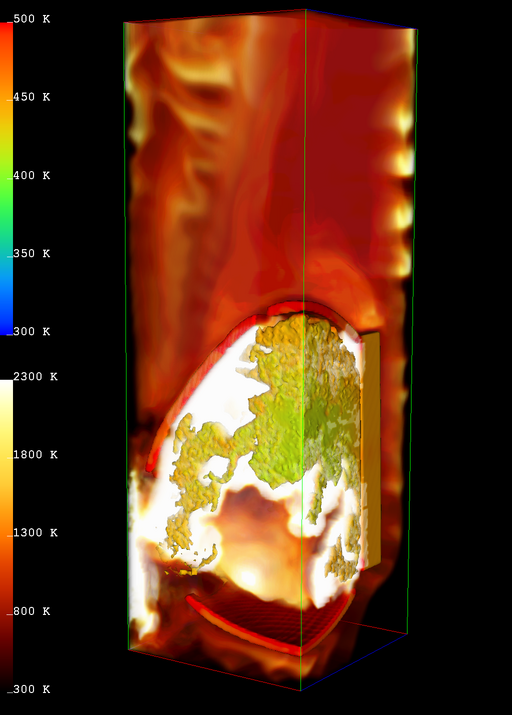
\includegraphics[width=\paperwidth,height=\paperheight,%
keepaspectratio]{fire-container-explosion-scirun.png}%
\vfill
}}}

\begin{document}

  %----------------------------------------------------------------------------------------
  %       TITLE PAGE
  %----------------------------------------------------------------------------------------
  \begingroup
    \thispagestyle{empty}
    \AddToShipoutPicture*{\BackgroundPic} % Image background
    \centering
    \vspace*{1cm}
    \par\normalfont\fontsize{35}{35}\sffamily\selectfont
    \textcolor{white}{MPM Theory Guide}\par % Book title
    \vspace*{0.5cm}
    {\Large \textcolor{white}{Vaango version 1.0}}\par
    \vspace*{1cm}
    {\Large \textcolor{white}{The Utah Uintah team}}\par % Author name
    {\Large \textcolor{white}{and}}\par % Author name
    {\Large \textcolor{white}{Biswajit Banerjee}}\par % Author name
  \endgroup

  %----------------------------------------------------------------------------------------
  %       COPYRIGHT PAGE
  %----------------------------------------------------------------------------------------

  \newpage
  ~\vfill
  \thispagestyle{empty}

  \noindent Copyright \copyright\ 2013 Callaghan Innovation\\ % Copyright notice
  \noindent Copyright \copyright\ 2015-2016 Parresia Research Limited\\ % Copyright notice

  %\noindent \textsc{Published by Publisher}\\ % Publisher

  %\noindent \textsc{book-website.com}\\ % URL

  %\noindent Licensed under the Creative Commons Attribution-NonCommercial 3.0 Unported License (the ``License''). You may not use this file except in compliance with the License. You may obtain a copy of the License at \url{http://creativecommons.org/licenses/by-nc/3.0}. Unless required by applicable law or agreed to in writing, software distributed under the License is distributed on an \textsc{``AS IS'' BASIS, WITHOUT WARRANTIES OR CONDITIONS OF ANY KIND}, either express or implied. See the License for the specific language governing permissions and limitations under the License.\\ % License information

  \noindent The contents of this manual can and will change significantly over time.  Please make sure that all the information is up to date.
  %\noindent \textit{First printing, March 2013} % Printing/edition date

  %----------------------------------------------------------------------------------------
  %       TABLE OF CONTENTS
  %----------------------------------------------------------------------------------------
  \chapterimage{fire-container-explosion-scirun-cut.png} % Table of contents heading image
  \pagestyle{empty} % No headers
  \tableofcontents % Print the table of contents itself
  \cleardoublepage % Forces the first chapter to start on an odd page so it's on the right
  \pagestyle{fancy} % Print headers again

%%
%% INTRODUCTION
%%
\setlength{\parindent}{0pt}
\setlength{\parskip}{5pt}

%
% Introduction to MPM
% Jim Guilkey/Biswajit Banerjee
% 03/25/2003
%
%
%\documentclass[10pt]{article}
%\usepackage[pdftex]{graphicx}
%\usepackage[dvips]{graphicx,epsfig}
%\usepackage{times}
%\usepackage{amsfonts}
%\usepackage{amsmath}
%\usepackage{amssymb}
%\usepackage{amstext}

%\topmargin 0.5in
%\headsep 0pt
%\headheight 0pt
%\oddsidemargin 0pt
%\evensidemargin 0pt
%\textheight 8.6in
%\textwidth 6.5in
%\columnsep 20pt
%\columnseprule 0.5pt
%\setlength{\parskip}{0.5em}
%\raggedright

%\newcommand{\tn}[1]{\mbox{\mathbf{#1}}}
%\newcommand{\sig}{\mbox{\boldmath $\sigma \!\!$ \unboldmath}}

%\title{An Introduction to the Material Point Method}
%\author{
%\\
%J.E. Guilkey \\
%Department of Mechanical Engineering \\
%University of Utah \\
%Salt Lake City, Utah 84112 \\
%\\
%}
%\date{}

%\begin{document}
%  \maketitle
%  \tableofcontents

\chapter{The Material Point Method}

  \section{Introduction}

The Material Point Method (MPM) as described by Sulsky, et al.
\cite{sulskycmame,sulskycpc} is a
particle method for structural mechanics simulations.  Solid 
objects
are represented by a collection of particles, or ``material 
points."  Each
of these particles carries with it information for that part of 
the
solid object that it represents.  This includes the mass, 
volume,
position, velocity and stress of that material.  MPM differs 
from other
so called ``mesh-free" particle methods in that, while each 
object is primarily 
represented by a collection of particles, a computational mesh 
is
also an important part of the calculation.  Particles do not 
interact
with each other directly, rather the particle information is 
interpolated
to the grid, where the equations of motion are integrated 
forward in time.
This time advanced solution is then used to update the particle 
state.
An example of two disks initially approaching each other 
represented by
material points on an overlying mesh is show in Figure \ref{fig-disks_init}.

\begin{figure}[h]
  \hspace{1.5in}
  \scalebox{0.5}{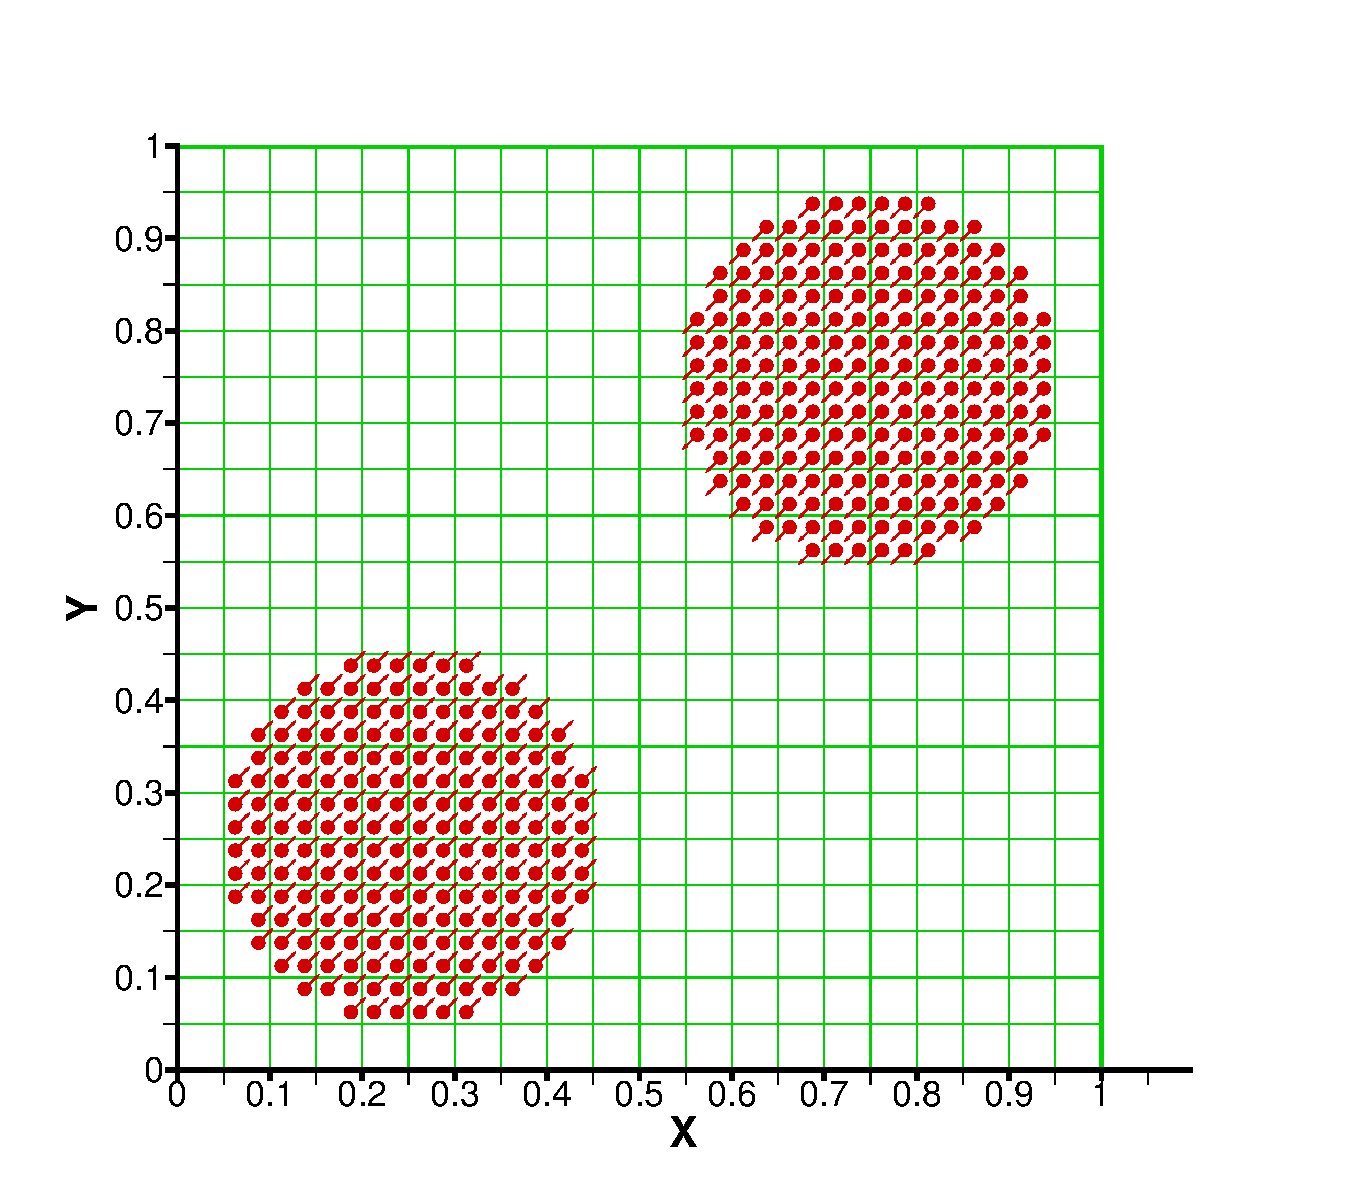
\includegraphics{disks.pdf}}
  %\epsfysize=3.5in
  %\epsfbox{Figures/disks.eps}
  \caption{\label{fig-disks_init} Initial particle representation of two
                                colliding disks on an overlying mesh.}
\end{figure}

The method usually uses a regular structured grid as a 
computational mesh.
While this grid, in principle, deforms as the material that it 
is representing
deforms, at the end of each timestep, it is reset to it's 
original undeformed
position, in effect providing a new computational grid for each 
timestep.
The use of a regular structured grid for each time step has a 
number of
computational advantages.  Computation of spatial gradients is 
simplified.
Mesh entanglement, which can plague fully Lagrangian techniques, 
such as
the Finite Element Method (FEM), is avoided.  MPM has also been 
successful
in solving problems involving contact between colliding objects, 
having an
advantage over FEM in that the use of the regular grid 
eliminates the
need for doing costly searches for contact surfaces\cite{bard}.

The choice of MPM over FEM as the C-SAFE structural mechanics method
was only in small part for the above mentioned criteria.  The
primary motivation was the ability to use MPM together with a multimaterial
CFD algorithm for solving tightly coupled fluid-structure interaction
problems.  This capability was first demonstrated in the CFDLIB
codes from Los Alamos by Bryan Kashiwa and co-workers.  There, as
in Uintah, MPM serves as the Lagrangian description of the solid
material in a multimaterial CFD code.  Certain elements of the
solution procedure are based in the Eulerian CFD algorithm, including
intermaterial heat and momentum transfer as well as satisfaction
of a multimaterial equation of state.  The use of a Lagrangian method
such as MPM to advance the solution of the solid material eliminates
the diffusion typically associated with Eulerian methods.

\section{Algorithm}

While a more detailed description of MPM can be found in 
\cite{sulskycpc},
the algorithm is laid out here.  The equations of motion are 
cast in the
form:

\begin{eqnarray}
	\tn{M}_g \cdot \tn{a}_g &=& \tn{Fext}_g - \tn{Fint}_g  
\label{newton2}
\end{eqnarray}
where $\tn{M}_g$ is the mass matrix, $\tn{a}_g$ is the 
acceleration vector,
$\tn{Fext}_g$ is the external force vector (sum of the body 
forces and
tractions), and $\tn{Fint}_g$ is the internal force vector 
resulting from
the divergence of the material stresses.  In general, $\tn{M}_g$ 
is a 
large, sparse matrix.  In practice, and in what follows here, a 
``lumped"
mass matrix is used, which only has entries on the diagonal, and 
is thus
represented as a column matrix.

The solution procedure begins by interpolating the particle 
state to the
grid, to form $\tn{M}_g$, $\tn{Fext}_g$, and to get a velocity 
on the grid
$\tn{v}_g$.  These quantities are calculated at each grid
node by the following equations:

\begin{eqnarray}
        \tn{M}_i &=& \sum_{p} S_{ip} m_p  
\label{expinterpolatemass}
\end{eqnarray}
\begin{eqnarray}
        \tn{v}_i &=& \frac{\sum\limits_{p} S_{ip} m_p 
\tn{v}_p}{\tn{M}_i} \label{expinterpolatevel}
\end{eqnarray}
\begin{eqnarray}
        \tn{Fext}_i &=& \sum_{p} S_{ip} \tn{Fext}_p. 
\label{expinterpolateFext}
\end{eqnarray}
$m_p$ is the particle
mass, $\tn{v}_p$ is the particle velocity, and $\tn{Fext}_p$ is 
the external
force on the particle.  The external force on the particle is 
generally an applied load of some type.  In Equation 
\ref{expinterpolatevel}, the numerator is the nodal momentum, 
which is then divided by the nodal mass to get a velocity.  
$S_{ip}$ is a ``shape function" for the $ith$ node
evaluated at $\tn{x}_p$.  Traditionally, the shape functions are 
multiplicative
combinations of one dimensional tent functions, as shown in
Figure \ref{fig-Sip}.  The shape functions serve to distance 
weight the contribution of each particle to the grid nodes.  

\begin{figure}[bh]
  \hspace{1.75in}
  \scalebox{0.7}{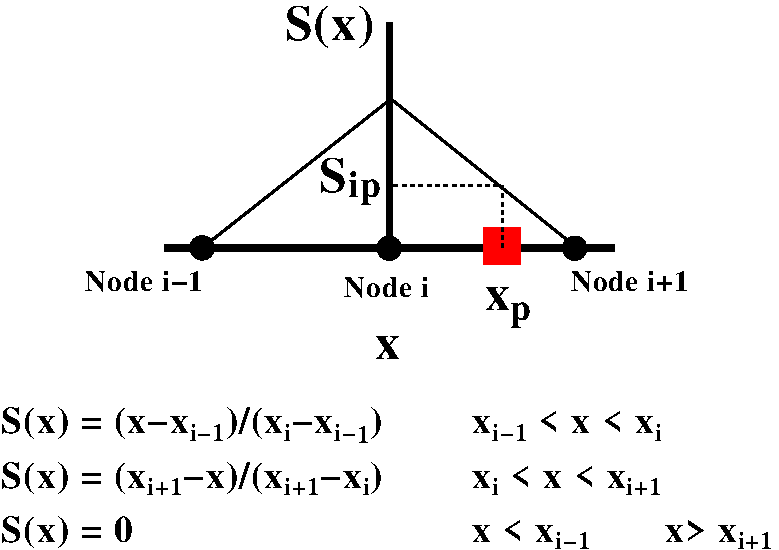
\includegraphics{Sip.pdf}}
  %\epsfysize=2.5in
  %\epsfbox{Figures/Sip.eps}
  \caption{\label{fig-Sip} One dimensional linear shape function, 
           $S(x)$.}
\end{figure}

At this point, a velocity gradient,  $\nabla \tn{v}_p$ is 
computed at
each particle using the grid velocities $\tn{v}_g$:

\begin{eqnarray}
	\nabla \tn{v}_p = \sum_i \tn{G}_{ip} \tn{v}_I
 \label{velgrad}
\end{eqnarray}

\noindent
where $\tn{G}_{ip}$ is the gradient of the $ith$ node's shape 
function,
evaluated at $\tn{x}_p$.  A one dimensional example of 
$\tn{G}_{ip}$ is
shown in Figure \ref{fig-Gip}.  Note that in going to multiple dimensions,
the $\tn{G}_{ip}$ are found by taking gradients of the multidimensional
$S_{ip}$ NOT by forming multiplicative combinations of the one-dimensional
$\tn{G}_{ip}$.

\begin{figure}[h]
  \hspace{1.75in}
  \scalebox{0.7}{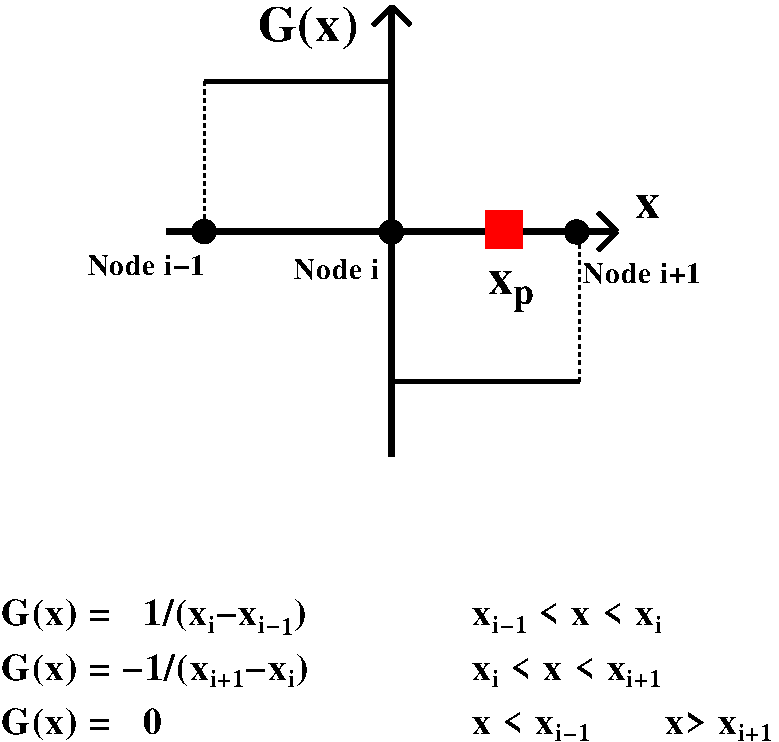
\includegraphics{Gip.pdf}}
  %\epsfysize=2.5in
  %\epsfbox{Figures/Gip.eps}
  \caption{\label{fig-Gip} One dimensional linear shape function 
           derivative, $G(x)$.}
\end{figure}
This velocity gradient is used as input to a constitutive model 
(stress-strain
relationship) which is evaluated at each particle.  The 
specifics of this 
calculation are dependent on the constitutive model.  An example 
of a simple elastic material model is described in the appendix.  
The result of this
calculation is the Cauchy stress at each particle, $\Bsig_p$.  
With this,
the internal force due to the divergence of the stress is 
calculated:

\begin{eqnarray}
	\tn{Fint}_g &=& \sum_{p} \tn{G}_{ip} \sig_p v_p
\end{eqnarray}

\noindent
where $v_p$ is the particle volume.  The internal force can be 
thought of as the force that holds a material together.  For a 
given deformation, this force is larger for stiffer materials.

Everything is now available to solve Equation \ref{newton2} for 
$\tn{a}_g$.
With that, the backward Euler method is used for all time 
integrations.
A convective grid velocity $\tn{v}^L_g$ is computed:

\begin{eqnarray}
	\tn{v}^L_g &=& \tn{v}_g  + \tn{a}_g dt
\end{eqnarray}

While the following calculation is never carried out, in 
principal, the
nodes of the grid also move with that convective velocity:

\begin{eqnarray}
	\tn{x}^L_g &=& \tn{x}_g  + \tn{v}^L_g dt     
\label{expdefgrid}
\end{eqnarray}

During this part of the computation, the particles move with the 
deforming
grid.  Their position and velocity is explicitly updated by:

\begin{eqnarray}
	\tn{v}_p (t + dt)  &=& \tn{v}_p (t)  + \sum_{i} S_{ip} 
\tn{a}_i  dt
\end{eqnarray}

\begin{eqnarray}
	\tn{x}_p (t + dt)  &=& \tn{x}_p (t)  + \sum_{i} S_{ip} 
\tn{v}^L_i  dt
\end{eqnarray}

This completes one timestep.  Note that not carrying out the 
calculation
in \ref{expdefgrid} explicitly has the effect of resetting the 
deformed
grid to it's undeformed position at the end of the timestep 
cycle.

As with all explicit time integration methods, a timestep size 
limit must
be enforced such that $dt < dx/(|\tn{v}_p| + c)$ for all 
particles, where $dx$ is the computational grid spacing and $c$ 
is the speed at which stress waves propagate through the 
material.
Failure to adhere to this condition will cause the solution to 
become
unstable and blow up.  The material wavespeed depends on the 
material model used, as well as on the particular parameters
chosen for that model.  Specifics of calculating the wavespeed
are given in the appendix.

%\bibliographystyle{unsrt}
%\bibliography{Bibliography}

\chapter{Elastic material models}
\section{Hyperelastic Material Models}

The subject of modeling the response of materials to deformation 
is a subject that has filled numerous textbooks.  Therefore, 
rather than attempt to condense these volumes, here the reader 
will be simply be given a simple material response model.  Other 
more complex material response models can be interchanged in the 
framework discussed above quite readily.

The author has come to prefer a class of models known as 
hyperelastic models.  What this means is that the stress 
response of these materials is derived from a strain energy 
function.  A strain energy function gives a relationship between 
the state of deformation that a material is in, and the amount 
of stored strain energy that this material has.  This is akin to 
the familiar relationship for the stored energy in a spring, 
$W=\frac{1}{2} k dx^2$ where k is the spring constant, and $dx$ is
the distance that the spring has been compressed or extended.

One such strain energy function is given by:

\begin{eqnarray}
	W &=& \frac{\lambda}{4}(J^2-1)
 - (\frac{\lambda}{2}+\mu) lnJ
+ \frac{\mu}{2}(trace(\tn{F}^T\tn{F} - 3)
\end{eqnarray}

from which the following relationship for the stress can be 
derived:

\begin{eqnarray}
       \sig &=& \frac{\lambda}{2}(J-\frac{1}{J})\tn{I} 
  + \mu (\tn{F}\tn{F}^T) - \tn{I})
 \label{stress}
\end{eqnarray}

where $\lambda$ and $\mu$ are material constants, while $J$ and 
$\tn{F}$ describe the state of deformation.  These will be 
defined shortly.

In the Algorithm section, the calculation of the velocity 
gradient, $\nabla \tn{v}_p$ is given in Equation \ref{velgrad}.
Starting from there, we can then compute an increment in the 
deformation gradient, $\tn{F}(dt)$ by:
\begin{eqnarray}
	\tn{F}(dt) &=& \nabla \tn{v}_p dt + \tn{I}.
\end{eqnarray}
This increment in the deformation gradient can then be used to 
compute a new total deformation gradient using:
\begin{eqnarray}
	\tn{F}(t+dt) &=& \tn{F}(dt) \tn{F}(t).
\end{eqnarray}
Note that the initial (t=0) deformation gradient is simply the 
identity, i.e. $\tn{F}(0) = \tn{I}$.  Now with the deformation 
gradient, one can compute $J$ by:
\begin{eqnarray}
	J &=& det(\tn{F}(t+dt)).
\end{eqnarray}

Note that $J$ represents the volumetric part of the deformation.  
Specifically, it is the ratio of the current volume of an 
element of material to it's original volume.  Similarly, we can
define an increment in $J$ as:
\begin{eqnarray}
	J_{inc} &=& det(\tn{F}(dt))
\end{eqnarray}
which  is the ratio of the current volume of an element of 
material to it's volume at the previous timestep.  Thus we can 
write:
\begin{eqnarray}
	v_p(t+dt) &=& J_{inc} v_p(t).
\end{eqnarray}

Elastic material properties are frequently given in terms of 
bulk and shear moduli, or $\kappa$ and $\mu$.  The shear is 
sometimes denoted by $G$.  The shear modulus $\mu$ appears in 
Equation \ref{stress} above.  $\lambda$ can be computed from
$\kappa$ and $\mu$ by:
\begin{eqnarray}
	\lambda &=& \kappa - \frac{2}{3}\mu.
\end{eqnarray}

Lastly, based on material properties $\lambda$ and $\mu$, a material 
wavespeed can be computed:

\begin{eqnarray}
	c^2 &=& (\lambda + 3 \mu)\frac{m_p}{v_p}.
\end{eqnarray}

This wavespeed can be used in computing the timestep size as 
described above.

\section{Other Material Models In the UCF}
Other material models implemented into the Uintah Computational
Framework (UCF) have been chosen for three purposes:
\begin{itemize}
  \item To verify the accuracy of the material point method (MPM)
        and to validate the coupling between the computational fluid 
        dynamics code (ICE) and MPM.
  \item To model the elastic-plastic deformation of the steel
        container and the consequent damage in the regimes of 
        both high and low strain rates and high and low temperatures.
  \item To model the polymer bonded explosive contained in the 
        container under various strain rates and temperatures.
\end{itemize}

\subsection{Material models for the validation of MPM}
The models that have been implemented for the verification of MPM
are:
\begin{itemize}
   \item Isotropic hypoelastic model using the Jaumann rate of 
         stress.
     \begin{enumerate}
        \item  MPM predictions have been compared with exact results 
               for thick cylinders under internal pressure for small
               strains, three-point beam bending, etc.
        \item  MPM predictions for the strain/stress contours for
               a set of disks in contact have been found to match
               experimental results.
     \end{enumerate}
   \item Isotropic hyperelastic material models for Mooney-Rivlin
         rubber and a modified compressible Neo-Hookean material. 
         Isotropic strain hardening plasticity for the Neo-Hookean
         material.
     \begin{enumerate}
        \item  A billet compression problem has been simulated using
               MPM and the results have been found to closely 
               match finite element simulations.
        \item  MPM simulations for a thick cylinder under internal
               pressure with plastic deformation (perfect plasticity)
               compare well with the exact solution.
     \end{enumerate}
\end{itemize}

\subsection{Material models for the container}
The material model for the steel container is used to determine
the state of stress in the container for an applied deformation
rate and deformation gradient at each material point.  The strain 
rates can vary from $10^{-3}$/s to $10^6$/s and temperatures in 
the container can vary from 250 K to 1000 K.  Plasticity dominates
the deformation of the container during the expansion of the 
explosive gases inside.  At high strain rates the volumetric
response of the container is best obtained using an equation of 
state.  After the plastic strain in the container
has reached a threshold value a damage/erosion model is required to
rupture the container.

Two plasticity models with strain rate and temperature dependency 
are the Johnson-Cook and the Mechanical Threshold Stress (MTS) 
models.  The volumetric response is calculated using a modified
Mie-Gruneisen equation of state.  A damage model that ties in well 
with the Johnson-Cook plasticity model is the Johnson-Cook damage 
model.  The erosion algorithm either removes the contribution
of the mass of the material point or forces the material point
to undergo no tension or shear under further loading.

The stress update at each material point is performed using either
of the two methods discussed below.
\begin{itemize}
   \item Isotropic Hypoelastic-plastic material model using an 
         additive decomposition of the rate of deformation tensor.
     \begin{enumerate}
        \item The rate of deformation tensor a material point
              is calculated using the grid velocities.
        \item An incremental update of the left stretch and the
              rate of rotation tensors is calculated.
        \item The stress and the rate of deformation are rotated
              into the material coordinates.
        \item A trial elastic deviatoric stress state is calculated.
        \item The flow stress is calculated using the plasticity
              model and compared with the vonMises yield condition.
        \item If the stress state is elastic, an update of the 
              stress is computed using the Mie-Gruneisen equation
              of state or the isotropic hypoelastic constitutive
              equation.
        \item If the stress state is plastic, all the strain rate 
              is considered to the plastic and an elastic correction
              along with a radial return step move the stress state
              to the yield surface.  The hydrostatic part of the 
              stress is calculated using the equation of state or
              the hypoelastic constitutive equation.
        \item A scalar damage parameter is calculated and used
              to determine whether material points are to be eroded
              or not.
        \item Stresses and deformation rates are rotated back to the
              laboratory coordinates.
     \end{enumerate}
   \item Isotropic Hyperelastic-plastic material model using a 
         multiplicative decomposition of the deformation gradient.
     \begin{enumerate}
        \item The velocity gradient at a material point
              is calculated using the grid velocities.
        \item An incremental update of the deformation gradient and
              the left Cauchy-Green tensor is calculated.
        \item A trial elastic deviatoric stress state is calculated
              assuming a compressible Neo-Hookean elastic model.
        \item The flow stress is calculated using the plasticity
              model and compared with the vonMises yield condition.
        \item If the stress state is elastic, an update of the 
              stress is computed using the Mie-Gruneisen equation
              of state or the compressible Neo-Hookean constitutive
              equation.
        \item If the stress state is plastic, all the strain rate 
              is considered to the plastic and an elastic correction
              along with a radial return step move the stress state
              to the yield surface.  The hydrostatic part of the 
              stress state is calculated using the Mie-Gruneisen
              equation of state or the Neo-Hookean model.
        \item A scalar damage parameter is calculated and used
              to determine whether material points are to be eroded
              or not.
     \end{enumerate}
\end{itemize}

The implementations have been tested against Taylor impact test data
for 4340 steel and HY 100 steel as well as one-dimensional problems
which have been compared with experimental stress-strain data.  At 
large tensile strains, material points tend to separate from the 
main body.  This issue is currently being explored and solutions are
being sought in the framework of MPM.

\subsection{Material models for the explosive}
The explosive is modeled using the ViscoSCRAM constitutive 
model.  Since large deformations or strains are not expected in 
the explosive, a small strain formulation has been implemented into 
the UCF.  The model consists of five generalized Maxwell elements
arranged in parallel, crack growth, friction at the crack 
interfaces and heating due to friction and reactions at the 
crack surfaces.  The implementation has been verified with 
experimental data and found to be accurate.

%\end{document}


\chapter{MPM Constitutive Models} \label{Sec:ConstitutiveModels}

The MPM code contains a large number of constitutive models that provide
a Cauchy stress on each particle based on the velocity gradient computed at
that particle.  The following is a list and very brief description of 
the most commonly used models.  The reader may wish to consult the
\tt inputs/MPM \normalfont and \tt inputs/MPMICE \normalfont directories
to find explicit examples of the use of these models, and others not
described in this section.

\clearpage
\section{Rigid Material}  This model was designed for use with the
\Textsfc{specified contact} model described in Section~\ref{Sec:Contact}.
It is designed to compute zero stress and identity deformation of the material,
and is basically a fast place-holder for materials that should not develop
any stress.

\begin{lstlisting}[language=XML]
  <constitutive_model type="rigid">
  </constitutive_model>
\end{lstlisting}

\begin{minipage}[t]{0.9\textwidth}
  \centering
  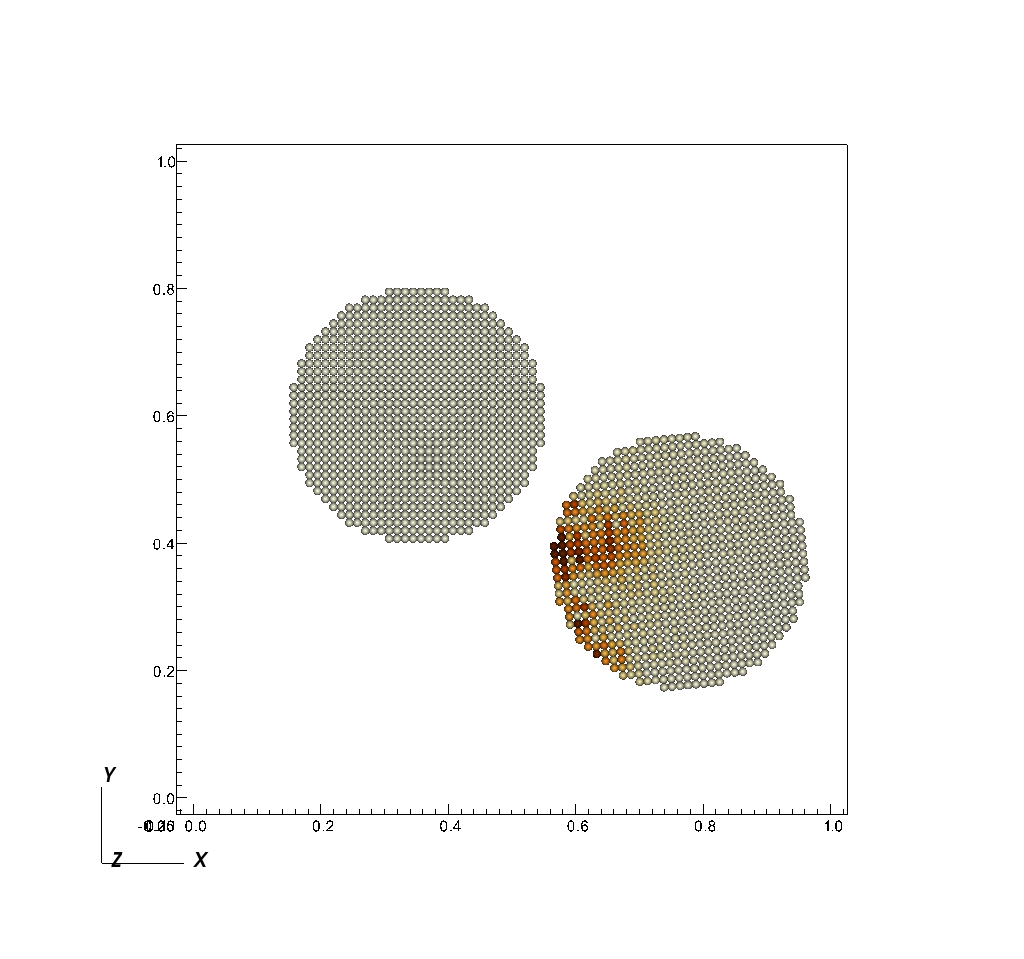
\includegraphics[width=0.5\columnwidth]{FIGS/contact/specified2.png}
  \captionof{figure}{A \Textsfc{rigid} disk (left) interacting with a deformable disk (right).}
\end{minipage}



\clearpage
\section{Ideal Gas}  This is simply an equation of state, with no shear stress.
Usage is given by:

\begin{lstlisting}
              <constitutive_model type="ideal_gas">
                  <specific_heat>  717.5        </specific_heat>
                  <gamma>  1.4        </gamma>
              </constitutive_model>
\end{lstlisting}


\clearpage
\section{Water}  This is a model for water, reported in \cite{water_model_ref}.
The P-V relationship is given by:
\begin{equation}
p=\kappa\left[\left(\frac{\rho}{\rho_0}\right)^{\gamma} - 1\right]
\end{equation}
Shear stress is simple Newtonian behavior.  It has not been validated,
but gives qualitatively reasonable behavior.  Usage is given by:
\begin{lstlisting}
              <constitutive_model type="water">
                 <bulk_modulus>15000.0</bulk_modulus>
                 <viscosity>.5</viscosity>
                 <gamma>7.0</gamma>
               </constitutive_model>
\end{lstlisting}


\clearpage
\section{Compressible Neo-Hookean Model} There are implementations of several
hyperelastic-plastic model described by Simo and Hughes\cite{Simo1998} (pp. 307 -- 321). 
 The model is dubbed "Unified Compressible Neo-Nookean Model" or UCNH for short.  Models can 
still be specified with old input file specifications, (i.e. comp\_neo\_hook, comp\_neo\_hook\_plastic,
cnh\_damage, cnhp\_damage) however these are merely wrappers for the underyling UCNH model.
 Plastic flow and failure can be modelled in addition to elasticity by  specifying 
several additional options with input flags. This models is very robust, and relatively 
straightforward because hyperelastic models don't require rotation back and forth 
between laboratory and material frames of reference.

NOTE: Support for Implicit CNH and CNH with specified solver is still lacking (for a short time).

The basic input section for UCNH:

\begin{lstlisting}
            <constitutive_model type="UCNH"> 
              <!-- Necessary flags for all CNH models -->
               <bulk_modulus>   8.9e9  </bulk_modulus>
               <shear_modulus>  3.52e9 </shear_modulus>
               <useModifiedEOS> true   </useModifiedEOS>
                
              <!-- Plasticity Parameters -->
               <usePlasticity>     true  </usePlasticity>
               <yield_stress>      100.0 </yield_stress>
               <hardening_modulus> 500.0 </hardening_modulus>
               <alpha>             1.0   </alpha>

            </constitutive_model>
\end{lstlisting}

A fairly sophisticated means of seeding explicit material heterogeneity is also provided for. 
To use these features the following four steps are required: 

1. To allow for failure (by material point erosion) the following must be set: 

In the \tt <MPM> \normalfont block, the erosion algorithm must be set to one of the following: 

\begin{lstlisting}
<erosion algorithm="AllowNoTension"/>
<erosion algorithm="AllowNoShear"/>
<erosion algorithm="ZeroStress"/>
\end{lstlisting}

In the \tt <constitutive\_model> \normalfont block:
\begin{lstlisting}
<useDamage>true</useDamage>
\end{lstlisting}

2. The failure surface type must be specified.  This is also in the \tt <constitutive\_model> \normalfont 
block.  One of the following must be specified:

\begin{lstlisting}
<failure_criteria>  MohrCoulomb </failure_criteria>
<failure_criteria>  MaximumPrincipalStress </failure_criteria>
<failure_criteria>  MaximumPrincipalStrain </failure_criteria>
\end{lstlisting}

The cohesion, $c$, is assigned using a distribution, as described below.  For the maximum 
principal stress and strain failure criteria, the cohesion is the maximum value of principal 
stress or strain that may be obtained (must be positive).  The MohrCoulomb failure criteria is
given by 
\begin{equation}
\frac{\sigma_3-\sigma_1}{2}=c\cos(\phi)-\frac{\sigma_3+\sigma_1}{2}\sin(\phi)
\end{equation}
where $\sigma_i$ are the ordered principal stresses, positive in tension 
($\sigma_3 > \sigma_2 > \sigma_1$).  Note, the MohrCoulomb failure 
surface also requires a friction angle, $\phi$, (in degrees):

\begin{lstlisting}
<friction_angle> friction angle </friction_angle>
\end{lstlisting}

A tensile cutoff failure surface may be added for MohrCoulomb.
The tensile cutoff is taken to be a fraction of the cohesion.  
This parameter is specified using:

\begin{lstlisting}
<tensile_cutoff_fraction> 0.1 </tensile_cutoff_fraction> 
\end{lstlisting}

Setting this to a large number effectively removes this failure surface, leaving just Mohr-Coulomb.

3. Material heterogeneity type must be specified.  For MohrCoulomb the cohesion is distributed 
spatially (an independent assignment for each material point).  For MaximumPrincipalStress and 
MaximumPrincipalStrain, the threshold stress or strain for failure, respectively, is distributed 
spatially (an independent assignment for each material point).  Material heterogeneity is 
distributed spatially by assigning values consistent with a distribution function.  Three different 
distributions may be used.  All parameters are in the \tt <constitutive\_model> \normalfont block:

\begin{lstlisting}
<failure_distrib> gauss </failure_distrib>
<failure_distrib> weibull </failure_distrib>
<failure_distrib> constant </failure_distrib>
\end{lstlisting}

A Gaussian (gauss) distribution requires the following parameters:

\begin{lstlisting}
<failure_mean> Gaussian mean value of cohesion </failure_mean>
<failure_std> Gaussian standard deviation of cohesion </failure_std>
<failure_seed> random number generator seed </failure_seed>
\end{lstlisting}

A Weibull (weibull) distribution requires the following parameters:
\begin{lstlisting}
<failure_mean> Weibull mean value of cohesion </failure_mean>
<failure_std> Weibull modulus </failure_std>
<failure_seed> random number generator seed </failure_seed>
\end{lstlisting}

A homogeneous (constant) assignment requires the following parameters:
\begin{lstlisting}
<failure_mean> value (all particles assigned one value) </failure_mean>
\end{lstlisting}

4. Distribution scaling with numerical resolution may optionally be specified.  This is only 
available for Gaussian and Weibull distributions.  All parameters are in the 
\tt <constitutive\_model> \normalfont block:

\begin{lstlisting}
<scaling> kayenta </scaling>
<scaling> none (default) </scaling>
\end{lstlisting}

For kayenta scaling, the mean value of the distribution is scaled by the factor
\begin{equation}
\biggl(\frac{\bar V}{V}\biggr)^{1/n}
\end{equation}
where $V$ is the particle volume, a function of numerical resolution.  The reference volume, 
$\bar V$ and exponent, $n$, both must be specified
\begin{lstlisting}
<reference_volume> $\bar V$ </reference_volume>
<exponent> n </exponent>
\end{lstlisting}
The exponent defaults to the Weibull modulus if the Weibull distribution is used.  This physically
motivated scaling provides for an increase in mean cohesion with decreasing particle size, generallly
consistent with the observation that smaller quantities of material contain fewer critical flaws.

\tt <comp\_neo\_hook> \normalfont is a basic elastic model, which calls the underlying \tt <UCNH> \normalfont .
The specifications for CNH are:

\begin{lstlisting}
          <constitutive_model type="comp_neo_hook">
               <bulk_modulus> 8.9e9  </bulk_modulus>
               <shear_modulus>3.52e9  </shear_modulus>
               <useModifiedEOS> true  </useModifiedEOS>
          </constitutive_model>
\end{lstlisting}

\tt <comp\_neo\_hook\_plastic> \normalfont as the constitutive model type,
 tells Uintah to use the basic elastic model extended
to include plasticity with isotropic linear hardening, 
which is equivalent to \tt <usePlasticity> \normalfont in UCNH.
The specifications for CNHP are:

\begin{lstlisting}
          <constitutive_model type="comp_neo_hook_plastic">
               <bulk_modulus> 8.9e9     </bulk_modulus>
               <shear_modulus>3.52e9    </shear_modulus>
               <useModifiedEOS> true    </useModifiedEOS>
               <yield_stress>100.0      </yield_stress>
               <hardening_modulus>500.0 </hardening_modulus>
               <alpha>     1.0          </alpha>
          </constitutive_model>
\end{lstlisting}


\tt <cnh\_damage> \normalfont as the constiutive model or \tt <useDamage> \normalfont 
tells Uintah to use a basic elastic model, with an extension
to failure based on a stress or strain as given below, thus yielding an
elastic-brittle failure model.  This model also allows a distribution
of failure strain (or stress) based on normal or Weibull distributions.
Note that the post-failure behaviour of simulations is not always robust.

The specification for CNHD are:

\begin{lstlisting}
            <constitutive_model type="cnh_damage"> 
               <bulk_modulus>   8.9e9  </bulk_modulus>
               <shear_modulus>  3.52e9 </shear_modulus>
               <useModifiedEOS> true   </useModifiedEOS>
                
            </constitutive_model>
\end{lstlisting}

When specifying \tt <cnh\_damage> \normalfont, the material heterogeneity and damage 
specification described for the general model (UCNH) may also be specified.

\tt <cnhp\_damage> \normalfont as the constitutive model (or both damage and plasticity
 flags discussed above) uses an extension
to failure based on a stress or strain as given below, thus yielding an
elastic-plastic model with failure.  Note that the post-failure behaviour of
simulations is not always robust.  The input section for damage and plasticity is
similar to that for UCNH without \tt <useDamage> \normalfont and \tt <usePlasticity>. \normalfont

When a particle has failed, the value of the particle variable \tt p.localized \normalfont
will be larger than one (0 means the particle has not failed) and can be output in the \tt DataArchiver
\normalfont section of the input file. In addition, the total number of failed particles as
a function of time \tt TotalLocalizedParticle \normalfont can be output. 

Another damage model that can be used with \tt <cnh\_damage> \normalfont and
\tt <cnhp\_damage> \normalfont is a subset of the brittle damage model of LS-DYNA's Concrete
 Model 159 (FHWA-HRT-057-062, 2007). The model is invoked by the following MPMFlag
\begin{lstlisting}
     <erosion algorithm="BrittleDamage"/>
\end{lstlisting}
in the \tt <MPM> \normalfont section of the input file. Two key features of the model are the use of
progressive (as opposed to sudden) damage due to softening to improve numerical stability, 
and the reduction of mesh size sensitivity via the specification of fracture energy. 

Brittle damage occurs when the mean stress $\sigma_{kk}/3$ is tensile
and the energy $\tau_b$, related to the maximum principal 
strain $\epsilon_{max}$, has exceeded a threshold value $r_0^b$

\begin{equation}
\sigma_{kk}>0, \phantom{ijkl}
\tau_b = \sqrt{E \epsilon_{max}^2} \geq r_0^b
\end{equation}
where $E$ is the Young's modulus. If at the next time step the mean stress is less than
zero (compressive), the damage mechanism can be optionally inactivated such that the current stress 
is set temporarily to a fraction of the undamaged stress to 
model stiffness recovery due to crack closing. When the mean stress becomes tensile again,
the value of the previous maximum damage $d$ can be restored; recovery is a user option in Uintah
but should be used with caution since stiffening is more prone to instability.
The softening function for brittle damage is assumed to be
\begin{equation}
d(\tau_b)= \frac{0.999}{D} \left(\frac{1+D}{1+D \exp^{-C(\tau_b-r_0^b)}} \right)
\end{equation}
where $C$ and $D$ are constants that define the shape of the softening
stress-strain curve.
  
To regulate mesh size sensitivity, the fracture energy
($G_f$), defined as the area under the stress-displacement
curve for displacement larger than $x_0$ (the displacement at peak strength), is to be maintained constant.
The user needs to input $G_f$ and $D$; $C$ is calculated internally. 

The maximum increment of damage that can accumulate over a single time
step is a user-defined input to avoid excessive damage accumulation over
a single time step to reduce numerical instability.

The brittle damage model is applicable to \tt <cnh\_damage> \normalfont and 
\tt <cnhp\_damage>. \normalfont For \tt cnh\_damage, \normalfont 
the parameters for brittle damage can be specified as

\begin{lstlisting}
                <constitutive_model type="cnh_damage">
               <shear_modulus>3.52e9</shear_modulus>
                 <bulk_modulus>8.9e9</bulk_modulus>
   <brittle_damage_initial_threshold>57.0 </brittle_damage_initial_threshold>
  <brittle_damage_fracture_energy>11.2</brittle_damage_fracture_energy>
  <brittle_damage_constant_D>0.1</brittle_damage_constant_D>
 <brittle_damage_max_damage_increment>0.1</brittle_damage_max_damage_increment>
<brittle_damage_allowRecovery> false </brittle_damage_allowRecovery>
<brittle_damage_recoveryCoeff> 1.0 </brittle_damage_recoveryCoeff>
   <brittle_damage_printDamage> false </brittle_damage_printDamage>
                </constitutive_model>

\end{lstlisting}

The tags in the input file for brittle damage are shown in the following table.

\begin{table}[ht]
\centering
\begin{tabular} {c c l}
\hline
Tag & Symbol & Description \\
\hline
brittle\_damage\_initial\_threshold & $r_0^b$ &  material property \\
brittle\_damage\_fracture\_energy & $G_f$ &  material property \\
brittle\_damage\_constant\_D & $D$ & material property \\
brittle\_damage\_max\_damage\_increment & & optional, default=0.1 \\
brittle\_damage\_allowRecovery & & allow crack closing (stiffening) \\
& & optional, default=false \\
brittle\_damage\_recoveryCoeff & & fraction of undamaged stress to recover\\
& & (between 0 and 1), optional\\
& & default=1.0 (full recovery) used only\\
& & when brittle\_damage\_allowRecovery \\
& & is set to true  \\
brittle\_damage\_printDamage & & print the state of damage \\
& & of damaged particles, default=false \\
& & (to reduce large amounts of output) \\
\hline
\end{tabular}
\end{table}

When a particle is damaged, the value of the particle variable \tt p.damage \normalfont
can be output in the \tt DataArchiver \normalfont section of the input file.



\clearpage

\section{Compressible Mooney-Rivlin Model} This model is generally parameterized
for rubber type materials.  Usage is as follows:
\begin{lstlisting}[language=XML]
              <constitutive_model type="comp_mooney_rivlin">
                 <he_constant_1>100000.0</he_constant_1>
                 <he_constant_2>20000.0</he_constant_2>
                 <he_PR>.49</he_PR>
               </constitutive_model>
\end{lstlisting}
where \tt <he\_constant\_(1,2)> \normalfont are usually referred to
as $C1$ and $C2$ in the literature.


\clearpage
\section{ElasticPlastic} The \tt <elastic\_plastic> \normalfont model is a
general purpose model that was primarily implemented for the purpose of
modeling high strain rate metal plasticity.  Dr. Biswajit Banerjee has
written an extensive description of the theory, implementation and use of
this model.  Because of the amount of detail involved, and because these
subtopics are interwoven, this model is given its own section below.


There is a large number remaining models but these are not frequently utilized. 
This includes models for viscoelasticity, soil models, and transverse isotropic materials (i.e., fiber reinforced composites).
Examples of their use can be found in the \tt inputs \normalfont directory.
Input files can also be constructed by checking the source code to see
what parameters are required.

There are a few models whose use is explicitly not recommended.  In particular,
\tt HypoElasticPlastic, Membrane and SmallStrainPlastic. \normalfont  Input
files calling for the first of these should be switched to the
\tt ElasticPlastic \normalfont model instead.

  \paragraph{Example input file for the HypoElasticPlastic model}
  An example of the portion of an input file that specifies a copper body
  with a hypoelastic stress update, Johnson-Cook plasticity model,
  Johnson-Cook Damage Model and Mie-Gruneisen Equation of State is shown
  below.
  \begin{lstlisting}
  <material>

    <include href="inputs/MPM/MaterialData/MaterialConstAnnCopper.xml"/>
    <constitutive_model type="elastic_plastic">
      <tolerance>5.0e-10</tolerance>
      <include href="inputs/MPM/MaterialData/IsotropicElasticAnnCopper.xml"/>
      <include href="inputs/MPM/MaterialData/JohnsonCookPlasticAnnCopper.xml"/>
      <include href="inputs/MPM/MaterialData/JohnsonCookDamageAnnCopper.xml"/>
      <include href="inputs/MPM/MaterialData/MieGruneisenEOSAnnCopper.xml"/>
    </constitutive_model>

    <geom_object>
      <cylinder label = "Cylinder">
        <bottom>[0.0,0.0,0.0]</bottom>
        <top>[0.0,2.54e-2,0.0]</top>
        <radius>0.762e-2</radius>
      </cylinder>
      <res>[3,3,3]</res>
      <velocity>[0.0,-208.0,0.0]</velocity>
      <temperature>294</temperature>
    </geom_object>

  </material>
  \end{lstlisting}

  The general material constants for copper are in the file
  \TT{MaterialConstAnnCopper.xml}.  The contents are shown below
  \begin{lstlisting}
  <?xml version='1.0' encoding='ISO-8859-1' ?>
  <Uintah_Include>
    <density>8930.0</density>
    <toughness>10.e6</toughness>
    <thermal_conductivity>1.0</thermal_conductivity>
    <specific_heat>383</specific_heat>
    <room_temp>294.0</room_temp>
    <melt_temp>1356.0</melt_temp>
  </Uintah_Include>
  \end{lstlisting}

  The elastic properties are in the file \TT{IsotropicElasticAnnCopper.xml}.
  The contents of this file are shown below.
  \begin{lstlisting}
  <?xml version='1.0' encoding='ISO-8859-1' ?>
  <Uintah_Include>
    <shear_modulus>45.45e9</shear_modulus>
    <bulk_modulus>136.35e9</bulk_modulus>
  </Uintah_Include>
  \end{lstlisting}

  The constants for the Johnson-Cook plasticity model are in the file
  \TT{JohnsonCookPlasticAnnCopper.xml}.  The contents of this file are
  shown below.
  \begin{lstlisting}
  <?xml version='1.0' encoding='ISO-8859-1' ?>
  <Uintah_Include>
    <flow_model type="johnson_cook">
      <A>89.6e6</A>
      <B>292.0e6</B>
      <C>0.025</C>
      <n>0.31</n>
      <m>1.09</m>
    </flow_model>
  </Uintah_Include>
  \end{lstlisting}

  The constants for the Johnson-Cook damage model are in the file
  \TT{JohnsonCookDamageAnnCopper.xml}.  The contents of this file are
  shown below.
  \begin{lstlisting}
  <?xml version='1.0' encoding='ISO-8859-1' ?>
  <Uintah_Include>
    <damage_model type="johnson_cook">
      <D1>0.54</D1>
      <D2>4.89</D2>
      <D3>-3.03</D3>
      <D4>0.014</D4>
      <D5>1.12</D5>
    </damage_model>
  </Uintah_Include>
  \end{lstlisting}

  The constants for the Mie-Gruneisen model (as implemented in the
  Uintah Computational Framework) are in the file
  \TT{MieGruneisenEOSAnnCopper.xml}.  The contents of this file are
  shown below.
  \begin{lstlisting}
  <?xml version='1.0' encoding='ISO-8859-1' ?>
  <Uintah_Include>
    <equation_of_state type="mie_gruneisen">
      <C_0>3940</C_0>
      <Gamma_0>2.02</Gamma_0>
      <S_alpha>1.489</S_alpha>
    </equation_of_state>
  </Uintah_Include>
  \end{lstlisting}

  As can be seen from the input file, any other plasticity model, damage
  model and equation of state can be used to replace the Johnson-Cook
  and Mie-Gruneisen models without any extra effort (provided the models
  have been implemented and the data exist).

  The material data can easily be taken from a material database or specified
  for a new material in an input file kept at a centralized location.  At this
  stage material data for a range of materials is kept in the directory
  \TT{.../Uintah/StandAlone/inputs/MPM/MaterialData}.


\subsection{Return Algorithms}

Two return algorithms are presently available.  Both assume the direction
of plastic flow is proportional to the current deviatoric stress.
  \begin{enumerate}
    \item Radial Return ({\bf default}).
    \item Modified Nemat-Nasser/Maudlin Return Algorithm.
  \end{enumerate}

\subsubsection{Radial Return Algorithm}
The plastic state is obtained using an iterative radial return
procedure as described in \cite{Simo98}, page 124, except that the
Newton procedure has been generalized to allow flow stresses to be
functions of both equivalent plastic strain and equivalent plastic
strain rate.

The rotated spatial rate of deformation tensor ($\Bd$) is additively
decomposed into an elastic part, $\Bd^e$, and a plastic part, $\Bd^p$,
  \begin{equation}
     \Bd = \Bd^e + \Bd^p
  \end{equation}
  It is convenient to work with the deviatoric parts of $\Bd$,
  $\Bd^e$, and $\Bd^p$, denoted $\Beta$, $\Beta^e$, and
  $\Beta^p$ respectively. The same additive decomposition obtains
  \begin{equation}
     \Beta = \Beta^e + \Beta^p
  \end{equation}
  Presently these models are limited to the case of plastic
  incompressibility ($\Tr{(\Bd^p)} = 0$), so that $\Bd^p=\Beta^p$.

The radial return algorithm assumes a yield condition of the form 
  \begin{equation}\label{eq:yield_condition}
    f(\Bs,\Ep,\dot{\Ep}) = \sqrt{3J_2} - \sigma_y(\Ep,\dot{\Ep})
  \end{equation}
where $\sigma_y$ is the flow stress, $J_2 = {1\over2}\Bs:\Bs$ is the
second invariant of the deviatoric part of the Cauchy stress, $\Bs$,
and the equivalent plastic strain is defined as
  \begin{equation}\label{eq:ep}
    \Ep = \int_0^t\sqrt{{2\over3}\Bd^p:\Bd^p}dt = \int_0^t\sqrt{{2\over3}\Beta^p:\Beta^p}dt
  \end{equation}
Assuming a state at the end of the previous time step, time $t^n$,
satisfying $f(\Bs^n,\Ep^n,\Epdot{}^n)\le0$, a new state satisfying
Eqn. \ref{eq:yield_condition} at time $t^{n+1}=t^n+\Delta t$, where
$\Delta t$ is the time step size, is sought.

Attention is further restricted to plastic flow associated with the yield condition,
Eqn. \ref{eq:yield_condition}, i.e.
  \begin{equation}\label{eq:associated_flow}
    \Bd^p = \Beta^p \propto \Partial{f}{\Bsig} = \lambdadot{\Bs\over\norm{\Bs}} = \lambdadot\Bn
  \end{equation}
where $\Bsig$ is the Cauchy stress , $\Bn={\Bs/\norm{\Bs}}$ and
$\lambdadot>0$ is a proportionality constant to be determined.
Attention is also restricted to isotropic materials, for which the
deviatoric response may be separated from the volumetric response.
The linear hypoelastic/plastic constitutive equation for deviatoric
response is
  \begin{equation}\label{eq:linearhypoelasticity}
    \dot{\Bs} = 2\mu(\Beta - \Beta^p)
  \end{equation}
where $\mu$ is the shear modulus.  The shear modulus is required to be
constant over the time step.  This permits evolution of the shear
modulus based on the state at the beginning of the time step using the
various shear modulus models described later, which are pressure and
temperature dependent.  It also allows for a visoelastic deviatoric
stress response provided an instantaneous shear modulus may be
defined, as described later in this section for linear
hypoviscoelasticity.

A trial stress is calculated assuming no plastic deformation, i.e.
  \begin{equation}\label{eq:strial}
    {\Bs^{\text{trial}}} = \Bs^n + 2\mu\Beta\Delta t
  \end{equation}
If $f(\Bs^{\text{trial}},\Ep^n,0)\le0$, the deformation is purely
elastic and the solution at time $t^{n+1}$ is
$\Bs^{n+1}=\Bs^{\text{trial}}$, $\Ep^{n+1}=\Ep^n$.  If
$f(\Bs^{\text{trial}},\Ep^n,0)>0$, the deformation is at least
partially plastic.  In this case
  \begin{equation}\label{eq:stress_update_0}
    \Bs^{n+1} = \Bs^n + \dot{\Bs}\Delta t
  \end{equation}
where $\dot{\Bs}$ is given by Eqn. \ref{eq:linearhypoelasticity}.
Eqn. \ref{eq:stress_update_0} may be rewritten in terms of the trial
stress
  \begin{equation}\label{eq:stress_update_1}
    \Bs^{n+1} = \Bs^{\text{trial}} - 2\mu\Beta^p\Delta t = \Bs^{\text{trial}} - 2\mu\lambdadot\Delta t {\Bs^{n+1}\over\norm{\Bs^{n+1}}}
  \end{equation}
using Eqn.s \ref{eq:strial}, \ref{eq:linearhypoelasticity} and
\ref{eq:associated_flow}.  This equation may be rearranged to give
  \begin{equation}
    \Bs^{\text{trial}} = \Bs^{n+1} \left[ 1 + {2\mu\lambdadot\Delta t\over\norm{\Bs^{n+1}}}\right]
  \end{equation}
which gives the key result that $\Bs^{\text{trial}} \propto
\Bs^{n+1}$, i.e. the trial stress and the updated stress are in the
same direction.  Consequently the flow direction may be written
  \begin{equation}\label{eq:flow_direction}
    \Bn={\Bs^{n+1}\over\norm{\Bs^{n+1}}}={\Bs^{\text{trial}}\over\norm{\Bs^{\text{trial}}}}
  \end{equation}
and Eqn. \ref{eq:stress_update_1} may be rewritten
  \begin{equation}\label{eq:stress_update_2}
    \Bs^{n+1} = \Bs^{\text{trial}} - 2\mu\lambdadot\Delta t \Bn
  \end{equation}
or, contracting both sides with $\Bn$, and using Eqn. \ref{eq:flow_direction},
  \begin{equation}
    \norm{\Bs^{n+1}} = \norm{\Bs^{\text{trial}}} - 2\mu\lambdadot\Delta t
  \end{equation}
which is a scalar equation for the proportionality constant
$\lambdadot$.  Using the yield condition
$f(\Bs^{n+1},\Ep^{n+1},\Epdot{}^{n+1})=0$
(Eqn. \ref{eq:yield_condition}), this equation may be written in terms
of $\lambdadot$
  \begin{equation}\label{eq:stress_update_3}
     \sqrt{2\over3}\sigma_y(\Ep^{n+1},\Epdot{}^{n+1}) = \norm{\Bs^{\text{trial}}} - 2\mu\lambdadot\Delta t
  \end{equation}
where from Eqn.s \ref{eq:ep} and \ref{eq:associated_flow},
$\Ep^{n+1}=\Ep^n+\sqrt{2\over3}\lambdadot\Delta t$ and $\dot{\Ep}^{n+1}=\sqrt{2\over3}\lambdadot$.

For the special case of linear isotropic hardening,
$\sigma_y(\Ep,\Epdot{})=\sigma_{y0}+k\Ep$, where $\sigma_{y0}$ is the
initial yield stress and $k$ is the hardening modulus,
Eqn. \ref{eq:stress_update_3} may be solved exactly.  More generally
the solution may be found using Newton iteration.  Defining
$\Delta\lambda = \lambdadot\Delta t$, and letting $j$ denote the
iteration, define
  \begin{equation}
     g(\Delta\lambda_j) = \norm{\Bs^{\text{trial}}} - 2\mu\Delta\lambda_j - \sqrt{2\over3}\sigma_y(\Epj^{n+1},\dot{\epsilon}_{p,j}^{n+1})
  \end{equation}
and, using the chain rule, the derivative may be calculated
  \begin{equation}
     {dg\over d\Delta\lambda}(\Delta\lambda_j) = - 2\mu - {2\over3}\left[{\partial\sigma_y\over \partial\Ep}(\Epj^{n+1},\dot{\epsilon}_{p,j}^{n+1}) + {\partial\sigma_y\over \partial{\dot{\epsilon}_{p,j}^{n+1}}}(\Epj^{n+1},\dot{\epsilon}_{p,j}^{n+1}){1\over\Delta t} \right]
  \end{equation}
Then until $|g(\Delta\lambda_{j+1})| < \text{TOL}$, calculate
  \begin{equation}
     \Delta\lambda_{j+1}=\Delta\lambda_j-{g(\Delta\lambda_j)\over{dg\over d\Delta\lambda}(\Delta\lambda_j)}
  \end{equation}
where $\Delta\lambda_0=0$, $\Epo^{n+1}=\Ep^n$,
$\dot{\epsilon}_{p,0}^{n+1}=0$, and, once $\Delta\lambda$ has been
determined to a specified accuracy, the final values of plastic strain
and strain rate are given by
  \begin{equation}
    \Ep^{n+1}=\Ep^n+\sqrt{2\over3}\Delta\lambda_{j+1}
  \end{equation}
  \begin{equation}
    \dot{\Ep}^{n+1}=\sqrt{2\over3}{\Delta\lambda_{j+1}\over\Delta t}
  \end{equation}
and the final value of $\Bs^{n+1}$ is calculated from Eqn. \ref{eq:stress_update_2}.

While several of the allowed flow stresses are of the form
$\sigma_y(\Ep,\dot{\Ep})$ as given in Eqn. \ref{eq:yield_condition},
others include temperature and/or pressure dependence.  Similarly,
several of the shear moduli models are functions of temperature and/or
pressure.  Using the radial return algorithm in these cases amounts to
convergence to the yield surface neglecting temperature changes, and
assuming a non-associated flow rule of the form in
Eqn. \ref{eq:associated_flow} (which is non-associated because the
pressure dependence of the flow stress has been neglected,
i.e. Eqn. \ref{eq:associated_flow} no longer holds).  This non
associated flow rule results in zero plastic dilation (actually
dilitation).  The end result is convergence to the flow stress with
temperature and pressure held constant, i.e. to
$\sigma_y(\Ep^{n+1},\dot{\Ep}^{n+1},p^n,T^n)$ with $\mu(p^n,T^n)$ and
no plastic dilitation.  While holding pressure and temperature fixed
over a time step is probably a good approximation for most explicit
calculations, non-associated flow may not be.

Finally, it was found that this return algorithm worked equally well
for linear hypoviscoelastic deviatoric response, i.e.
  \begin{equation}\label{eq:linearhypoviscoelasticity}
    \dot{\Bs} = 2\mu(\Beta - \Beta^p) - \sum_{i=1}^N {\Bs_i\over \tau_i}
  \end{equation}
rather than Eqn. \ref{eq:linearhypoelasticity}.
Eqn. \ref{eq:linearhypoviscoelasticity} is the constitutive equation
for $N$ linear Maxwell elements in parallel, each with shear modulus
$\mu_i$, time constant $\tau_i$, and deviatoric stress $\Bs_i$, and
  \begin{equation}
    \Bs = \sum_{i=1}^N \Bs_i \quad\quad \mu = \sum_{i=1}^N \mu_i
  \end{equation}
This model is detailed in the Deviatoric Stress Models section.
Combined with a yield condition, the combination results in a
model for viscoplastic material response.

The radial return algorith is the {\bf default}, and also may be
explicitely invoked with the tag
  \begin{lstlisting}[language=XML]
    <plastic_convergence_algo>radialReturn</plastic_convergence_algo>
  \end{lstlisting}

\subsubsection{Modified Nemat-Nasser/Maudlin Return Algorithm}

This stress update algorithm is a slightly modified version of the
approach taken by Nemat-Nasser et
al. (1991,1992)~\cite{Nemat91,Nemat92}, Wang (1994)~\cite{Wang94},
Maudlin (1996)~\cite{Maudlin96}, and Zocher et
al. (2000)~\cite{Zocher00}.  It is presently only documented in the
code itself.  It is also known to give erroneous results under uniaxial
stress conditions.

The modified Nemat-Nasser/Maudlin return algorith is invoked with
the tag
  \begin{lstlisting}[language=XML]
    <plastic_convergence_algo>biswajit</plastic_convergence_algo>
  \end{lstlisting}
{\it This is an experts only algorithm!!!}


\subsection{Hypo-Elastic Plasticity in Uintah}  \label{Sec:ElasticPlastic}

The hypoelastic-plastic stress update is a mix and match combination
of isotropic models.  The equation of state may be varied
independently of the deviatoric response.  For elastic deviatoric
response the shear moduli may be taken to be functions of temperature
and pressure.  Plasticity is based on an additive decomposition of the
rate of deformation tensor into elastic and plastic parts.
Incompressibility is assumed for plastic deformations, i.e. the
plastic strain rate is proportional to the deviatoric stress.  Various
yield conditions and flow stresses may be mixed and matched.  There
are also options for damage/melting modeling.  {\it Note that there
  are few checks to prevent users from mixing and matching
  inappropriate models}.

Additional models can be added to this framework.  Presently, the
material models available are:
\begin{enumerate}
    \item Adiabatic Heating and Specific Heat:
      \begin{itemize}
        \item Taylor-Quinney coefficient.
        \item Constant Specific Heat ({\bf default}).
        \item Cubic Specific Heat.
        \item Specific Heat for Copper.
        \item Specific Heat for Steel.
      \end{itemize}
    \item The equation of state (pressure/volume response):
      \begin{itemize}
        \item Hypoelastic ({\bf default}).
        \item Neo-Hookean.
        \item Mie-Gruneisen.
      \end{itemize}
    \item The deviatoric stress model:
      \begin{itemize}
        \item Linear hypoelasticity ({\bf default}).
        \item Linear hypoviscoelasticity.
      \end{itemize}
    \item The melting model:
      \begin{itemize}
        \item Constant melt temperature ({\bf default}).
        \item Linear melt temperature.
        \item Steinberg-Cochran-Guinan (SCG) melt.
        \item Burakovsky-Preston-Silbar (BPS) melt.
      \end{itemize}
    \item Temperature and pressure dependent shear moduli (only works
      with linear hypoelastic deviatoric stress model):
      \begin{itemize}
        \item Constant shear modulus ({\bf default}).
        \item Mechanical Threshold Stress (MTS) model.
        \item Steinberg-Cochran-Guinan (SCG) model.
        \item Nadal-LePoac (NP) model.
        \item Preston-Tonks-Wallace (PTW) model.
      \end{itemize}
    \item The yield condition:
      \begin{itemize}
        \item von Mises.
        \item Gurson-Tvergaard-Needleman (GTN).
      \end{itemize}
    \item The flow stress:
      \begin{itemize}
        \item the Isotropic Hardening model
        \item the Johnson-Cook (JC) model
        \item the Steinberg-Cochran-Guinan-Lund (SCG) model.
        \item the Zerilli-Armstrong (ZA) model.
        \item the Zerilli-Armstrong for polymers model.
        \item the Mechanical Threshold Stress (MTS) model.
        \item the Preston-Tonks-Wallace (PTW) model.
      \end{itemize}
    \item The plastic return algorithm:
      \begin{itemize}
        \item Radial Return ({\bf default}).
        \item Modified Nemat-Nasser/Maudlin.
      \end{itemize}
    \item The damage model:
      \begin{itemize}
        \item Johnson-Cook damage model.
      \end{itemize}
\end{enumerate}

This model is invoked using
  \begin{lstlisting}[language=XML]
      <constitutive_model="elastic_plastic_hp">
        <shear_modulus>0.2845e4</shear_modulus>
        <bulk_modulus>1.41e4</bulk_modulus>
        <initial_material_temperature>298</initial_material_temperature>
        <plastic_convergence_algo>radialReturn</plastic_convergence_algo>
        <taylor_quinney_coeff> 0.9 </taylor_quinney_coeff>

        submodels

      </constitutive_model>
  \end{lstlisting}
  where ``submodels'' indicates subsets of tags corresponding to the
  listed above (and detailed below).  {\it Note that the specified
    bulk and shear moduli are used to calcuate a stable time step size
    for the first time step (hence it is important that they be
    consistent with EOS and deviatoric stress submodel material
    constants).  However, if the default EOS and/or deviatoric stress
    models are used, then these material constants are sufficient for
    bulk and/or deviatoric stress response, and are automatically used
    in those models.}  The bulk modulus is also used to determine
  artificial viscosity parameters (throughout the simulation).


  \subsection{Adiabatic Heating and Specific Heat}
  A part of the plastic work done is converted into heat and used to update the
  temperature of a particle.  The increase in temperature ($\Delta T$) due to
  an increment in plastic strain ($\Delta\epsilon_p$) is given by the equation
  \begin{equation}
    \Delta T = \cfrac{\chi\sigma_y}{\rho C_p} \Delta \epsilon_p
  \end{equation}
  where $\chi$ is the Taylor-Quinney coefficient, and $C_p$ is the specific
  heat.  The value of the Taylor-Quinney coefficient is taken to be 0.9
  in all our simulations (see \cite{Ravi01} for more details on the
  variation of $\chi$ with strain and strain rate).

  The Taylor-Quinney coefficient is taken as input in the ElasticPlastic model
  using the tags
  \begin{lstlisting}[language=XML]
    <taylor_quinney_coeff> 0.9 </taylor_quinney_coeff>
  \end{lstlisting}

  \subsubsection{Default specific heat model}
  The default model returns a constant specific heat and is invoked using
  \begin{lstlisting}[language=XML]
    <specific_heat_model type="constant_Cp">
    </specific_heat_model>
  \end{lstlisting}

  \subsubsection{Cubic specific heat model}
  The specific heat model is of the form \cite{Menikoff2003}:
  \Beq
    C_v = \frac{\tilde{T}^3}{c_3\tilde{T}^3+c_2\tilde{T}^2+c_1\tilde{T}+c_0} 
  \Eeq
  where $\tilde{T}$ is the reduced temperature, and $c_0$-$c_3$ are fit parameters.
  The reduced temperature is calculated using $\tilde{T}=T/\theta (V)$ and the
  Debye temperature is:
  \Beq
    \theta (V)=\theta_0\left(\frac{V_0}{V}\right)^ae^{b\left(V_0-V\right)/V}
  \Eeq
  where $V$ is the specific volume and $\theta_0$ is the reference Debye temperature and
  a and b are fit parameters.
  The constant pressure specific heat is calculated via:
  \Beq
    C_p = C_v+\beta^2TVK_T
  \Eeq
  where $\beta$ and $K_T$ are the volumetric expansion coefficeint and 
  isothermal bulk modulus respectively.
  
  The model is invoked using:
  \begin{lstlisting}[language=XML]
    <specific_heat_model type="cubic_Cp">
      <a> 1.0 </a>
      <b> 1.0 </b>
      <beta> 1.0 </beta>
      <c0> 1.0 </c0>
      <c1> 1.0 </c1>
      <c2> 1.0 </c2>
      <c3> 1.0 </c3>
    </specific_heat_model>
  \end{lstlisting}
  where all parameters but $\beta$, $a$ and $b$ are required.


  \subsubsection{Specific heat model for copper}
  The specific heat model for copper is of the form
  \Beq
    C_p =
    \begin{cases}
      A_0~T^3 - B_0~T^2 + C_0~T - D_0 & \text{if} ~~T < T_0 \\
      A_1~T + B_1 & \text{if} ~~T \ge T_0 ~.
    \end{cases}
  \Eeq
  The model is invoked using
  \begin{lstlisting}[language=XML]
  <specific_heat_model type = "copper_Cp"> </specific_heat_model>
  \end{lstlisting}

  \subsubsection{Specific heat model for steel}
  A relation for the dependence of $C_p$ upon temperature is
  used for the steel (\cite{Lederman74}).
  \begin{align}
    C_p & = \begin{cases}
            A_1 + B_1~t + C_1~|t|^{-\alpha} & \text{if}~~ T < T_c \\
            A_2 + B_2~t + C_2~t^{-\alpha^{'}} & \text{if}~~ T > T_c 
          \end{cases} \label{eq:CpSteel}\\
    t & = \cfrac{T}{T_c} - 1 
  \end{align}
  where $T_c$ is the critical temperature at which the phase transformation
  from the $\alpha$ to the $\gamma$ phase takes place, and $A_1, A_2, B_1, B_2,
  \alpha, \alpha^{'}$ are constants.

  The model is invoked using
  \begin{lstlisting}[language=XML]
  <specific_heat_model type = "steel_Cp"> </specific_heat_model>
  \end{lstlisting}

  The heat generated at a material point is conducted away at the end of a
  time step using the transient heat equation.  The effect of conduction on
  material point temperature is negligible (but non-zero) for the high
  strain-rate problems simulated using Uintah.

\subsection{Equation of State Models}
The elastic-plastic stress update assumes that the volumetric part of
the Cauchy stress can be calculated using an equation of state.  There
are three equations of state that are implemented in Uintah.  These
are
\begin{enumerate}
    \item A default hypoelastic equation of state.
    \item A neo-Hookean equation of state.
    \item A Mie-Gruneisen type equation of state.
\end{enumerate}

\subsubsection{Default hypoelastic equation of state}
In this case we assume that the stress rate is given by
\Beq
    \dot{\Bsig} = \lambda~\Tr(\Bd^e)~\Bone + 2~\mu~\Bd^e
\Eeq
where $\Bsig$ is the Cauchy stress, $\Bd^e$ is the elastic part of
the rate of deformation, and $\lambda, \mu$ are constants.

If $\Beta^e$ is the deviatoric part of $\Bd^e$ then we can write
\Beq
    \dot{\Bsig} = \left(\lambda + \frac{2}{3}~\mu\right)~\Tr(\Bd^e)~\Bone +
        2~\mu~\Beta^e = \kappa~\Tr(\Bd^e)~\Bone + 2~\mu~\Beta^e ~.
\Eeq
If we split $\Bsig$ into a volumetric and a deviatoric part, i.e.,
$\Bsig = p~\Bone + \Bs$ and take the time derivative to get
$\dot{\Bsig} = \dot{p}~\Bone + \dot{\Bs}$ then
\Beq
    \dot{p} = \kappa~\Tr(\Bd^e) ~.
\Eeq
In addition we assume that $\Bd = \Bd^e + \Bd^p$.  If we also assume that
the plastic volume change is negligible, we can then write that
\Beq
    \dot{p} = \kappa~\Tr(\Bd) ~.
\Eeq
This is the equation that is used to calculate the pressure $p$ in the
default hypoelastic equation of state, i.e.,
\Beq
    \boxed{
    p_{n+1} = p_n + \kappa~\Tr(\Bd_{n+1})~\Delta t ~.
    }
\Eeq
To get the derivative of $p$ with respect to $J$, where $J = \det(\BF)$,
we note that
\Beq
    \dot{p} = \Partial{p}{J}~\dot{J} = \Partial{p}{J}~J~\Tr(\Bd) ~.
\Eeq
Therefore,
\Beq
    \boxed{
    \Partial{p}{J} = \cfrac{\kappa}{J} ~.
    }
\Eeq

This model is invoked in Uintah using
\begin{lstlisting}[language=XML]
  <equation_of_state type="default_hypo">
  </equation_of_state>
\end{lstlisting}
The code is in \tt.../MPM/ConstitutiveModel/PlasticityModels/DefaultHypoElasticEOS.cc \normalfont
If an EOS is not specified then this model is the {\bf default}.

\subsubsection{Default hyperelastic equation of state}
In this model the pressure is computed using the relation
\begin{equation}
  p = \Half~\kappa~\left(J^e - \cfrac{1}{J^e}\right)
\end{equation}
where $\kappa$ is the bulk modulus and $J^e$ is determinant of the elastic
part of the deformation gradient.

We can also compute
\begin{equation}
  \Deriv{p}{J} = \Half~\kappa~\left(1 + \cfrac{1}{(J^e)^2}\right) ~.
\end{equation}

This model is invoked in Uintah using
\begin{lstlisting}[language=XML]
  <equation_of_state type="default_hyper">
  </equation_of_state>
\end{lstlisting}
The code is in \TT{.../MPM/ConstitutiveModel/PlasticityModels/HyperElasticEOS.cc}.

\subsubsection{Mie-Gruneisen equation of state}
The pressure ($p$) is calculated using a Mie-Gr{\"u}neisen equation of state
\begin{equation} \label{eq:MG}
  p = p_{ref} +\rho \Gamma (e - e_{ref})
\end{equation}
where $\rho$ is the mass density, $\Gamma$ the Gr{\"u}neisen parameter (unitless) and $p_{ref}$
and $e_{ref}$ are known pressure and internal specific energy on a reference curve {\it and are a function
of volume only}.  As the form can be formally viewed as an expansion valid near the reference curve,
ideally the reference curve prescribes states near those of interest.  The reference curve could be
the shock Hugoniot, the standard adiabat (through the initial state), the 0 K isotherm, the isobar $p=0$,
the curve $e=0$, or some composite of these curves to cover the range of interest.  

For shock calculations it makes sense to use the Hugoniot as a reference curve.  We Assume the following
relationship between shock wave velocity, $U_s$ and particle velocity,  $U_p$,
\begin{equation} \label{eq:SteinbergUsUp}
  U_s = C_0 + s_\alpha U_p + s_2 \frac{U_p^2}{U_s} + s_3 \frac{U_p^3}{U_s^2}
\end{equation}
where $C_0$ is the bulk speed of sound, and the $s$'s are dimensionless coefficients.
This form is due to Steinberg (\cite{Steinberg91}), and is a straight--forward extension to a nonlinear 
shock velocity, particle velocity relationship.  It reduces to the linear relationship most frequently 
used, e.g. (\cite{Wilkins99,Zocher00}), with $s_2 = s_3 = 0$.  Using the steady shock jump conditions for
conservation of mass, momentum and energy, the Hugoniot reference pressure, $p_H$ and specific energy,
$e_H$ may be determined
\begin{equation} \label{eq:pH}
  p_H = \frac{\rho_0 C_0^2 \eta}{1 - s_\alpha \eta - s_2 \eta^2 - s_3 \eta^3}
\end{equation}
\begin{equation} \label{eq:eH}
  e_H = \frac{p_H \eta}{2 \rho_0}
\end{equation}
where $\rho_0$ is the initial density (pre-shock) and
\begin{equation} \label{eq:eta}
  \eta = 1-\frac{\rho_0}{\rho}
\end{equation}
is a measure of volumetric deformation.  Using these relationships and the additional assumption that
$\rho\Gamma=\rho_0\Gamma_0$ the Mie-Gr{\"u}neisen equation of state may be written
\begin{equation} \label{eq:EOSMG_upd}
  \boxed{
  p =  \frac{\rho_0~C_0^2~\eta(1-\frac{\Gamma_0\eta}{2})}{(1 - s_\alpha \eta - s_2 \eta^2 - s_3 \eta^3)^2}
           + \rho_0\Gamma_0~e
  }
\end{equation}
To extend the Mie Gr{\"u}neisen EOS into tensile stress regimes, for $\eta<0$ the pressure is evaluated as
\begin{equation} \label{eq:EOSMG_upd_1}
  \boxed{
  p =  \rho_0~C_0^2~\eta + \rho_0\Gamma_0~e
  }
\end{equation}
This equation is integrated explicitly, using beginning timestep values for energy and the current value
of density to update the pressure.  For isochoric plasticity,
\begin{equation*}
  J^e = J = \det(\BF) = \cfrac{\rho_0}{\rho} ~.
\end{equation*}
where $\BF^e$ is the elastic part of the deformation gradient.  
The increment in specific internal energy is computed using
  \begin{equation}
    \rho^* \Delta e = (\sigma^*_{ij} D_{ij} - q D_{kk}) \Delta t
  \end{equation}
where $\sigma^*_{ij}$ and $\rho^*$ are the average stress and density over the time step, 
$D_{ij}$ is the rate of deformation tensor, and $q$ is
the artificial viscosity.  Note that the artificial velocity term must be included explicitly
since it is not accumulated in the total stress.

The temperature, $T$, is calculated using the thermodynamic relationship
  \begin{equation}\label{eq:dTthermo}
    dT = -\rho\Gamma T dv + \frac{TdS}{C_v}
  \end{equation}
where $v$ is the specific volume, $S$ the entropy and $C_v$ the specific heat at constant volume.
Entropy change is associated with irreversible, or dissipative, processes.  Equating $TdS$ to the
dissipated work terms, those components of temperature change are computed in the appropriate routines,
such as plasticity or artificial viscosity.  In fact, not all of the dissipated energy needs be
converted to heat, as allowed for by using the Taylor--Quinney coefficient (see below).  The first term
in \label{eq:dT} may be integrated to give the isentropic temperature change
  \begin{equation}\label{eq:dTisentropic}
    \Delta T_{isentropic} = -T\Gamma_0\frac{\rho_0}{\rho}D_{kk}\Delta t
  \end{equation}
where the same assumption, $\rho\Gamma=\rho_0\Gamma_0$ is used.  The isentropic temperature change
is computed as part of the EOS response.

Should an implicit integration scheme be used the tangent moduli are needed, which in turn require calculation of
\Beq
  \boxed{
  \Partial{p}{J^e} =
  \cfrac{\rho_0~C_0^2~[1 + (S_{\alpha}-\Gamma_0)~(1-J^e)]}
        {[1-S_{\alpha}~(1-J^e)]^3} - \Gamma_0~\Partial{e}{J^e}.
  }
\Eeq
We neglect the $\Partial{e}{J^e}$ term in our calculations.  {\it Note: this calculation hasn't been updated for
the Steinberg nonlinear shock velocity, particle velocity relationship.}

This model is invoked in Uintah using
\begin{lstlisting}[language=XML]
  <equation_of_state type="mie_gruneisen">
    <C_0>5386</C_0>
    <Gamma_0>1.99</Gamma_0>
    <S_alpha>1.339</S_alpha>
    <S_2>1.339</S_2>
    <S_3>1.339</S_3>
  </equation_of_state>
\end{lstlisting}
The code is in \TT{.../MPM/ConstitutiveModel/PlasticityModels/MieGruneisenEOS.cc}.

It is worth noting that this approach to calculating energy and temperature is not necessarily consistent
with existing implementations.  In fact, it does not appear that there is a standard approach, many shock
codes have unique implementations.  In particular, it appears that the elastic stored energy term is 
often neglected, as well as the isentropic temperature change.

It is worth noting that the approach outlined above is consistent with that taken fairly
recently by Wilkins (\cite{Wilkins99}).  Wilkins expands the pressure and energy as polynomials in $\eta$
and uses Hugoniot data (and a linear $U_s$, $U_p$ relationship) to determine the coefficients.  Using the
additional thermodynamic relationship
  \begin{equation}\label{eq:de}
    de = -p dv + TdS
  \end{equation}
and substituting for $TdS$ from \ref{eq:dTthermo}, assuming $C_v$ constant and 
$\rho\Gamma=\rho_0\Gamma_0$ (as in Wilkins), the following relationship may be derived
  \begin{equation}\label{eq:e}
    e = -\int_{v_0}^v (p - \rho_0 \Gamma_0 C_v T) dv + C_v(T-T_0)
  \end{equation}
Since the integral is for $dS=0$, it may be integrated to give an alternate form of \ref{eq:dTisentropic},
  \begin{equation}\label{eq:dTisentropic2}
    T_{isentropic} = T_0\exp(\Gamma_0(1-\frac{\rho_0}{\rho}))
  \end{equation}
which may be substituted into \ref{eq:e} along with the expansion for $p(\eta)$ (here for $s_2=s_3=0$)
  \begin{equation}\label{eq:pofeta}
    p = \rho_0\Gamma_0 e + \rho_0 C_0^2(\eta + (2s_\alpha-\frac{\Gamma_0}{2})\eta^2 + s_\alpha(3s_\alpha-\Gamma_0)\eta^3) + O(\eta^4)
  \end{equation}
to give the equation
  \begin{equation}\label{eq:e2}
    e+\int_{v_0}^v\rho_0\Gamma_0 e dv = C_v(T-T_0) + \rho_0 \Gamma_0C_vT_0\int_{v_0}^v \exp(\Gamma_0\eta)dv 
       -\rho_0\Gamma_0\int_{v_0}^v(\eta + (2s_\alpha-\frac{\Gamma_0}{2})\eta^2 + s_\alpha(3s_\alpha-\Gamma_0)\eta^3)dv
  \end{equation}
Finally, using 
  \begin{equation}
    e = e_0(\eta) + \int_{T_0}^T C_vdT
  \end{equation}
with a polynomial expansion for $e(\eta)$ in powers of $\eta$, \ref{eq:e2} can be integrated 
to determine the coefficients in the expansion.  Determining the coefficients this way gives 
exactly the same expansion for energy as derived in
Wilkins, using a different approach.  The advantages of the approach outlined above are it's relative simplicity,
and generality -- no assumption of constant specific heat is needed.

\subsection{Deviatoric Stress Models}
The elastic-plastic stress update assumes that the deviatoric part of
the Cauchy stress can be calculated independently of the equation of
state.  There are two deviatoric stress models that are implemented in
Uintah.  These are
\begin{enumerate}
    \item A default hypoelastic deviatoric stress.
    \item A linear hypoviscooelastic deviatoric stress.
\end{enumerate}

\subsubsection{Default Hypoelastic Deviatoric Stress}
  In this case the stress rate is given by
  \begin{equation}
    \dot{\Bs} = 2\mu(\Beta - \Beta^p)
  \end{equation}
  where $\mu$ is the shear modulus.  This model is invoked using
  \begin{lstlisting}[language=XML]
      <deviatoric_stress_model type="hypoElastic">
      </deviatoric_stress_model>
  \end{lstlisting}
  If a deviatoric stress model is not specified then this model is the
  {\bf default}.

\subsubsection{Linear Hypoviscoelastic Deviatoric Stress}
  This model is a three--dimensional version of a Generalized Maxwell
  model, as presented in \cite{Zerilli2007}.  It is specifically
  implemented to be combined with the ZA for Polymers Flow Stress
  Model described previously.  Together these models combine into a
  hypoviscoplastic model.  The stress update is given by
  \begin{equation}
    \dot{\Bs} = 2\mu(\Beta - \Beta^p) - \sum_{i=1}^N \frac{\Bs_i}{\tau_i}
  \end{equation}
  where $\mu$ is the shear modulus and $\Bs_i$ are maxwell element
  stresses which are tracked internally.  Also
  \begin{equation}
    \Bs = \sum_{i=1}^N \Bs_i \quad\quad \mu = \sum_{i=1}^N \mu_i
  \end{equation}
  This model is invoked using
  \begin{lstlisting}[language=XML]  
      <deviatoric_stress_model type="hypoViscoElastic">
        <mu> [3.0, 5.0, 7.0] </mu>
        <tau> [1.67, 10.7, 107.0] </tau>
      </deviatoric_stress_model>
  \end{lstlisting}
where the number of elements in arrays mu and tau must be the same.

\subsection{Melting Temperature}
  \subsubsection{Default model}
  The default model is to use a constant melting temperature.  This model
  is invoked using
  \begin{lstlisting}
      <melting_temp_model type="constant_Tm">
      </melting_temp_model>
  \end{lstlisting}

  \subsubsection{Linear melt model}
  A melting temperature model designed to be linear in pressure can be invoked using
  \begin{lstlisting}
      <melting_temp_model type="linear_Tm">
        <T_m0> </T_m0>
        <a>   </a>
        <b> </b>
        <Gamma_0> </Gamma_0>
        <K_T> </K_T>
      </melting_temp_model>
  \end{lstlisting}

  where T\_m0 is required, and either a or Gamma\_0 along with K\_T, or b.  
  T\_m0 is the initial melting temperature in Kelvin, a is the Kraut-Kennedy coefficient,
  Gamma\_0 is the Gruniesen Gamma, b is the pressure coefficient in Kelvin per Pascal, and K\_T
  is the isothermal bulk modulus in Pascals.
  The pressure is calculated using either
  \begin{equation}
    T_{m}=T_{m0}+bP
  \end{equation}
  or
  \begin{equation}
    T_{m}=T_{m0}\left(1+a\frac{\rho_0}{\rho}\right)
  \end{equation}
  The constants in these equations are linked together via the following equation
  \begin{equation}
   b=\frac{aT_{m0}}{K_T}
  \end{equation}
  and a is related to the Gruneisen Gamma by the Lindemann Law \cite{Poirier91}:
  \begin{equation}
   a=2\left(\Gamma_0-\frac{1}{3}\right)
  \end{equation}

  

  \subsubsection{SCG melt model}
  We use a pressure dependent relation to determine the melting
  temperature ($T_m$).  The Steinberg-Cochran-Guinan (SCG) melt model
  (\cite{Steinberg80}) has been used for our simulations of copper.
  This model is based on a modified Lindemann law and has the form
  \begin{equation} \label{eq:TmSCG}
    T_m(\rho) = T_{m0} \exp\left[2a\left(1-\frac{1}{\eta}\right)\right]
              \eta^{2(\Gamma_0-a-1/3)}; \quad
    \eta = \frac{\rho}{\rho_0}
  \end{equation}
  where $T_{m0}$ is the melt temperature at $\eta = 1$,
  $a$ is the coefficient of the first order volume correction to
  Gr{\"u}neisen's gamma ($\Gamma_0$).

  This model is invoked with
  \begin{lstlisting}
    <melting_temp_model type="scg_Tm">
      <T_m0> 2310.0 </T_m0>
      <Gamma_0> 3.0 </Gamma_0>
      <a> 1.67 </a>
    </melting_temp_model>
  \end{lstlisting}

  \subsubsection{BPS melt model}
  An alternative melting relation that is based on dislocation-mediated
  phase transitions - the Burakovsky-Preston-Silbar (BPS) model
  (\cite{Burakovsky00}) can also be used.  This model has been used to
  determine the melt temperature for 4340 steel.  The BPS model has the form
  \begin{align}
    T_m(p) & = T_m(0)
      \left[\cfrac{1}{\eta} + 
            \cfrac{1}{\eta^{4/3}}~\cfrac{\mu_0^{'}}{\mu_0}~p\right]~; 
    \quad
    \eta = \left(1 + \cfrac{K_0^{'}}{K_0}~p\right)^{1/K_0^{'}} 
    \label{eq:TmBPS}\\
    T_m(0) & = \cfrac{\kappa\lambda\mu_0~v_{WS}}{8\pi\ln(z-1)~k_b}
               \ln\left(\cfrac{\alpha^2}{4~b^2\rho_c(T_m)}\right)
  \end{align}
  where $p$ is the pressure, $\eta = \rho/\rho_0$ is the compression,
  $\mu_0$ is the shear modulus at room temperature and zero pressure,
  $\mu_0^{'} = \partial\mu/\partial p$ is the derivative of the shear modulus
  at zero pressure, $K_0$ is the bulk modulus at room temperature and
  zero pressure, $K_0^{'} = \partial K/\partial p$ is the derivative of the
  bulk modulus at zero pressure, $\kappa$ is a constant, $\lambda = b^3/v_{WS}$
  where $b$ is the magnitude of the Burgers' vector, $v_{WS}$ is the
  Wigner-Seitz volume, $z$ is the coordination number, $\alpha$ is a
  constant, $\rho_c(T_m)$ is the critical density of dislocations, and
  $k_b$ is the Boltzmann constant.

  This model is invoked with
  \begin{lstlisting}
    <melting_temp_model type="bps_Tm">
      <B0> 137e9 </B0>
      <dB_dp0> 5.48 <dB_dp0>
      <G0> 47.7e9 <G0>
      <dG_dp0> 1.4 <dG_dp0>
      <kappa> 1.25 <kappa>
      <z> 12 <z>
      <b2rhoTm> 0.64 <b2rhoTm>
      <alpha> 2.9 <alpha>
      <lambda> 1.41 <lambda>
      <a> 3.6147e-9<a>
      <v_ws_a3_factor> 1/4 <v_ws_a3_factor>
      <Boltzmann_Constant> <Boltzmann_Constant>
    </melting_temp_model>
  \end{lstlisting}

  \subsection{Shear Modulus} \label{sec:ModelShear}
  Three models for the shear modulus ($\mu$) have been tested in our
  simulations.  The first has been associated with the Mechanical
  Threshold Stress (MTS) model and we call it the MTS shear model.
  The second is the model used by Steinberg-Cochran-Guinan and we call
  it the SCG shear model while the third is a model developed by
  Nadal and Le Poac that we call the NP shear model.

  \subsubsection{Default model}
  The default model gives a constant shear modulus.  The model is
  invoked using
  \begin{lstlisting}
    <shear_modulus_model type="constant_shear">
    </shear_modulus_model>
  \end{lstlisting}

  \subsubsection{MTS Shear Modulus Model}
  The simplest model is of the form suggested by \cite{Varshni70}
  (\cite{Chen96})
  \begin{equation} \label{eq:MTSShear}
    \mu(T) = \mu_0 - \frac{D}{exp(T_0/T) - 1}
  \end{equation}
  where $\mu_0$ is the shear modulus at 0K, and $D, T_0$ are material
  constants.

  The model is invoked using
  \begin{lstlisting}
    <shear_modulus_model type="mts_shear">
      <mu_0>28.0e9</mu_0>
      <D>4.50e9</D>
      <T_0>294</T_0>
    </shear_modulus_model>
  \end{lstlisting}

  \subsubsection{SCG Shear Modulus Model}
  The Steinberg-Cochran-Guinan (SCG) shear modulus
  model (\cite{Steinberg80,Zocher00}) is pressure dependent and
  has the form
  \begin{equation} \label{eq:SCGShear}
    \mu(p,T) = \mu_0 + \Partial{\mu}{p} \frac{p}{\eta^{1/3}} +
         \Partial{\mu}{T}(T - 300) ; \quad
    \eta = \rho/\rho_0
  \end{equation}
  where, $\mu_0$ is the shear modulus at the reference state($T$ = 300 K,
  $p$ = 0, $\eta$ = 1), $p$ is the pressure, and $T$ is the temperature.
  When the temperature is above $T_m$, the shear modulus is instantaneously
  set to zero in this model.

  The model is invoked using
  \begin{lstlisting}
  <shear_modulus_model type="scg_shear">
    <mu_0> 81.8e9 </mu_0>
    <A> 20.6e-12 </A>
    <B> 0.16e-3 </B>
  </shear_modulus_model>
  \end{lstlisting}

  \subsubsection{NP Shear Modulus Model}
  A modified version of the SCG model has been developed by
  \cite{Nadal03} that attempts to capture the sudden drop in the
  shear modulus close to the melting temperature in a smooth manner.
  The Nadal-LePoac (NP) shear modulus model has the form
  \begin{equation} \label{eq:NPShear}
    \mu(p,T) = \frac{1}{\mathcal{J}(\That)}
      \left[
        \left(\mu_0 + \Partial{\mu}{p} \cfrac{p}{\eta^{1/3}} \right)
        (1 - \That) + \frac{\rho}{Cm}~k_b~T\right]; \quad
    C := \cfrac{(6\pi^2)^{2/3}}{3} f^2
  \end{equation}
  where
  \begin{equation}
    \mathcal{J}(\That) := 1 + \exp\left[-\cfrac{1+1/\zeta}
        {1+\zeta/(1-\That)}\right] \quad
       \text{for} \quad \That:=\frac{T}{T_m}\in[0,1+\zeta],
  \end{equation}
  $\mu_0$ is the shear modulus at 0 K and ambient pressure, $\zeta$ is
  a material parameter, $k_b$ is the Boltzmann constant, $m$ is the atomic
  mass, and $f$ is the Lindemann constant.

  The model is invoked using
  \begin{lstlisting}
    <shear_modulus_model type="np_shear">
      <mu_0>26.5e9</mu_0>
      <zeta>0.04</zeta>
      <slope_mu_p_over_mu0>65.0e-12</slope_mu_p_over_mu0>
      <C> 0.047 </C>
      <m> 26.98 </m>
    </shear_modulus_model>
  \end{lstlisting}

  \subsubsection{PTW Shear model}
  The PTW shear model is a simplified version of the SCG shear model.
  The inputs can be found in \TT{.../MPM/ConstitutiveModel/PlasticityModel/PTWShear.h}.


\subsection{Yield conditions}
When failure is to be simulated we can use the
Gurson-Tvergaard-Needleman yield condition instead of the von Mises
condition.

  \subsubsection{The von Mises yield condition}
  The von Mises yield condition is the default.  It specifies a yield condition of
  the form
  \begin{equation}
    \Phi = \sqrt{3J_2} - \sigma_y
  \end{equation}
  where $J_2$ is the second invariant of the deviatoric stress tensor
  ($J_2=\tfrac{1}{2}\Bs:\Bs$) and $\sigma_y$ is the flow stress. Currently
  the return algorithms are restricted to plastic flow in the
  direction of the deviatoric stress
  (Eqn. \ref{eq:associated_flow}). See the discussion in the Radial
  Return algorithm description for details.  The von Mises yield
  condition is invoked using the tags
  \begin{lstlisting}[language=XML]
    <yield_condition type="vonMises">
    </yield_condition>
  \end{lstlisting}

  \subsubsection{The Gurson-Tvergaard-Needleman (GTN) yield condition}
  The Gurson-Tvergaard-Needleman (GTN) yield
  condition~\cite{Gurson1977,Tver1984} depends on porosity.  {\it This
  model is for experts only!!!}  Here are some caveats: Formally,
  you can replace the flow stress in Gurson’s model with the flow
  stresses of Johnson-Cook, ZA, etc., but the internal variable
  updates would have to be modified extensively.  For example, the JC
  yield stress depends on the equivalent plastic strain, but this
  needs to be the equivalent plastic strain of the matrix material,
  which is very different from the equivalent plastic strain of the
  porous composite. For example, under pure hydrostatic compression at
  the macroscale, the matrix material will suffer massive amounts of
  plastic SHEAR strains at the microscale (even though, for
  hydrostatic loading, it has zero plastic shear strain at the
  macroscale) and thus would need to harden. While the models should
  run, they are unlikely to give realistic results.

  The GTN yield condition is a fairly good bound in compression but a
  TERRIBLE bound in tension (in fact using it in tension can produce
  non-physical predictions of negative plastic work tantamount to
  tension causing pore COLLAPSE; very few Gurson implementations catch
  this problem because very few of them include run-time checks of
  solution quality, including this one).

  The GTN yield condition will not work with Radial Return.  An error
  will be generated in this case.  Presently it only runs with the
  modified Nemat-Nasser/Maudlin return algorithm.  Plastic flow is
  assumed to be in the direction of deviatoric stress.  Hence this
  is nonassociated flow for this pressure dependent yield condition.

  The GTN yield condition can be written as
  \begin{equation}
    \Phi = \left(\frac{\sigma_{eq}}{\sigma_f}\right)^2 +
    2 q_1 f_* \cosh \left(q_2 \frac{Tr(\sigma)}{2\sigma_f}\right) -
    (1+q_3 f_*^2) = 0
  \end{equation}
  where $q_1,q_2,q_3$ are material constants and $f_*$ is the porosity
  (damage) function given by
  \begin{equation}
    f* = 
    \begin{cases}
      f & \text{for}~~ f \le f_c,\\ 
      f_c + k (f - f_c) & \text{for}~~ f > f_c 
    \end{cases}
  \end{equation}
  where $k$ is a constant and $f$ is the porosity (void volume fraction).  The
  flow stress in the matrix material is computed using either of the two
  plasticity models discussed earlier.  Note that the flow stress in the matrix
  material also remains on the undamaged matrix yield surface and uses an
  associated flow rule.

  This yield condition is invoked using
  \begin{lstlisting}[language=XML]
    <yield_condition type="gurson">
      <q1> 1.5 </q1>
      <q2> 1.0 </q2>
      <q3> 2.25 </q3>
      <k> 4.0 </k>
      <f_c> 0.05 </f_c>
    </yield_condition>
  \end{lstlisting}

  \subsubsection{Porosity model}
  The evolution of porosity is calculated as the sum of the rate of growth
  and the rate of nucleation~\cite{Ramaswamy1998a}.  The rate of growth of
  porosity and the void nucleation rate are given by the following equations
  ~\cite{Chu1980}
  \begin{align}
    \dot{f} &= \dot{f}_{\text{nucl}} + \dot{f}_{\text{grow}} \\
    \dot{f}_{\text{grow}} & = (1-f) \text{Tr}(\BD_p) \\
    \dot{f}_{\text{nucl}} & = \cfrac{f_n}{(s_n \sqrt{2\pi})}
            \exp\left[-\Half \cfrac{(\epsilon_p - \epsilon_n)^2}{s_n^2}\right]
            \dot{\epsilon}_p
  \end{align}
  where $\BD_p$ is the rate of plastic deformation tensor, $f_n$ is the volume
  fraction of void nucleating particles , $\epsilon_n$ is the mean of the
  distribution of nucleation strains, and $s_n$ is the standard
  deviation of the distribution.

  The inputs tags for porosity are of the form
  \begin{lstlisting}[language=XML]
    <evolve_porosity> true </evolve_porosity>
    <initial_mean_porosity>         0.005 </initial_mean_porosity>
    <initial_std_porosity>          0.001 </initial_std_porosity>
    <critical_porosity>             0.3   </critical_porosity>
    <frac_nucleation>               0.1   </frac_nucleation>
    <meanstrain_nucleation>         0.3   </meanstrain_nucleation>
    <stddevstrain_nucleation>       0.1   </stddevstrain_nucleation>
    <initial_porosity_distrib>      gauss </initial_porosity_distrib>
  \end{lstlisting}



\subsection{Flow Stress}
  We have explored seven temperature and strain rate dependent
  models that can be used to compute the flow stress.  Some of these are also
  pressure dependent (note that plastic flow does is non-associative for
  pressure dependent models):
  \begin{enumerate}
    \item the Isotropic Hardening model
    \item the Johnson-Cook (JC) model
    \item the Steinberg-Cochran-Guinan-Lund (SCG) model.
    \item the Zerilli-Armstrong (ZA) model.
    \item the Zerilli-Armstrong for polymers model.
    \item the Mechanical Threshold Stress (MTS) model.
    \item the Preston-Tonks-Wallace (PTW) model.
  \end{enumerate}

  \subsubsection{Isotropic Hardening Flow Stress Model}
  The Isotropic Hardening model is a simple linear relationship for the flow stress
  \begin{equation}
    \sigma_y(\Ep) = \sigma_y + K (\Ep)
  \end{equation}
  where $\Ep$ is the equivalent plastic strain, $\sigma_y$ and $k$ are material constants.

  The inputs for this model are
  \begin{lstlisting}[language=XML]
  <flow_model type="isotropic_hardening">
    <sigma_Y>792.0e6</sigma_y>
    <K>510.0e6</K>
  </flow_model>
  \end{lstlisting}

  \subsubsection{JC Flow Stress Model}
  The Johnson-Cook (JC) model (\cite{Johnson1983}) is purely empirical and gives
  the following relation for the flow stress ($\sigma_y$)
  \begin{equation}
    \sigma_y(\Ep,\Epdot{},T) = 
    \left[A + B (\Ep)^n\right]\left[1 + C \ln(\Epdot{}^{*})\right]
    \left[1 - (T^*)^m\right]
  \end{equation}
  where $\Ep$ is the equivalent plastic strain, $\Epdot{}$ is the
  plastic strain rate, A, B, C, n, m are material constants,
  \begin{equation}
    \Epdot{}^{*} = \cfrac{\Epdot{}}{\Epdot{0}}; \quad
    T^* = \cfrac{(T-T_0)}{(T_m-T_0)}~,
  \end{equation}
  $\Epdot{0}$ is a user defined plastic strain rate,
  $T_0$ is a reference temperature, and $T_m$ is the melt temperature.
  For conditions where $T^* < 0$, we assume that $m = 1$.

  The inputs for this model are
  \begin{lstlisting}[language=XML]
  <flow_model type="johnson_cook">
    <A>792.0e6</A>
    <B>510.0e6</B>
    <C>0.014</C>
    <n>0.26</n>
    <m>1.03</m>
    <T_r>298.0</T_r>
    <T_m>1793.0</T_m>
    <epdot_0>1.0</epdot_0>
  </flow_model>
  \end{lstlisting}

  \subsubsection{SCG Flow Stress Model}
  The Steinberg-Cochran-Guinan-Lund (SCG) model is a semi-empirical model
  that was developed by \cite{Steinberg1980} for high strain rate
  situations and extended to low strain rates and bcc materials by
  \cite{Steinberg1989}.  The flow stress in this model is given by
  \begin{equation}\label{eq:SCGL}
    \sigma_y(\Ep,\Epdot{},T) = 
     \left[\sigma_a f(\Ep) + \sigma_t (\Epdot{}, T)\right]
     \frac{\mu(p,T)}{\mu_0} 
  \end{equation}
  where $\sigma_a$ is the athermal component of the flow stress,
  $f(\Ep)$ is a function that represents strain hardening,
  $\sigma_t$ is the thermally activated component of the flow stress,
  $\mu(p,T)$ is the shear modulus, and $\mu_0$ is the shear modulus
  at standard temperature and pressure.  The strain hardening function
  has the form
  \begin{equation}
    f(\Ep) = [1 + \beta(\Ep + \Epi)]^n ; \quad
    \sigma_a f(\Ep) \le \sigma_{\text{max}}
  \end{equation}
  where $\beta, n$ are work hardening parameters, and $\Epi$ is the
  initial equivalent plastic strain.  The thermal component $\sigma_t$
  is computed using a bisection algorithm from the following equation (based
  on the work of \cite{Hoge1977})
  \begin{equation}
    \Epdot{} = \left[\frac{1}{C_1}\exp\left[\frac{2U_k}{k_b~T}
      \left(1 - \frac{\sigma_t}{\sigma_p}\right)^2\right] + 
      \frac{C_2}{\sigma_t}\right]^{-1}; \quad
    \sigma_t \le \sigma_p
  \end{equation}
  where $2 U_k$ is the energy to form a kink-pair in a dislocation segment
  of length $L_d$, $k_b$ is the Boltzmann constant, $\sigma_p$ is the Peierls
  stress. The constants $C_1, C_2$ are given by the relations
  \begin{equation}
    C_1 := \frac{\rho_d L_d a b^2 \nu}{2 w^2}; \quad
    C_2 := \frac{D}{\rho_d b^2}
  \end{equation}
  where $\rho_d$ is the dislocation density, $L_d$ is the length of a
  dislocation segment, $a$ is the distance between Peierls valleys,
  $b$ is the magnitude of the Burgers' vector, $\nu$ is the Debye frequency,
  $w$ is the width of a kink loop, and $D$ is the drag coefficient.

  The inputs for this model are of the form
  \begin{lstlisting}[language=XML]
    <flow_model type="steinberg_cochran_guinan">
      <mu_0> 81.8e9 </mu_0>
      <sigma_0> 1.15e9 </sigma_0>
      <Y_max> 0.25e9 </Y_max>
      <beta> 2.0 </beta>
      <n> 0.50 </n>
      <A> 20.6e-12 </A>
      <B> 0.16e-3 </B>
      <T_m0> 2310.0 </T_m0>
      <Gamma_0> 3.0 </Gamma_0>
      <a> 1.67 </a>
      <epsilon_p0> 0.0 </epsilon_p0>
    </flow_model>
  \end{lstlisting}

  \subsubsection{ZA Flow Stress Model}
  The Zerilli-Armstrong (ZA) model (\cite{Zerilli1987,Zerilli1993,Zerilli2004})
  is based on simplified dislocation mechanics.  The general form of the
  equation for the flow stress is
  \begin{equation}
    \sigma_y(\Ep,\Epdot{},T) = 
      \sigma_a + B\exp(-\beta(\Epdot{}) T) + 
                           B_0\sqrt{\Ep}\exp(-\alpha(\Epdot{}) T)
  \end{equation}
  where $\sigma_a$ is the athermal component of the flow stress given by
  \begin{equation}
    \sigma_a := \sigma_g + \frac{k_h}{\sqrt{l}} + K\Ep^n,
  \end{equation}
  $\sigma_g$ is the contribution due to solutes and initial dislocation
  density, $k_h$ is the microstructural stress intensity, $l$ is the
  average grain diameter, $K$ is zero for fcc materials,
  $B, B_0$ are material constants.  The functional forms of the exponents
  $\alpha$ and $\beta$ are
  \begin{equation}
    \alpha = \alpha_0 - \alpha_1 \ln(\Epdot{}); \quad
    \beta = \beta_0 - \beta_1 \ln(\Epdot{}); 
  \end{equation}
  where $\alpha_0, \alpha_1, \beta_0, \beta_1$ are material parameters that
  depend on the type of material (fcc, bcc, hcp, alloys).  The Zerilli-Armstrong
  model has been modified by \cite{Abed2005} for better performance at high
  temperatures.  However, we have not used the modified equations in our
  computations.

  The inputs for this model are of the form
  \begin{lstlisting}[language=XML]
    
    <flow_model type="zerilli_armstrong">
       <sigma_g>     50.0e6   </sigma_g>
       <k_H>         5.0e6    </k_H>
       <sqrt_l_inv>  5.0      </sqrt_l_inv>
       <B>           25.0e6   </B>
       <beta_0>      0.0      </beta_0>
       <beta_1>      0.0      </beta_1>
       <B_0>         0.0      </B_0>
       <alpha_0>     0.0      </alpha_0>
       <alpha_1>     0.0      </alpha_1>
       <K>           5.0e9    </K>
       <n>           1.0      </n>
     </flow_model>
  \end{lstlisting}

  \subsubsection{ZA for Polymers Flow Stress Model}
  The Zerilli-Armstrong flow stress model for polymers(\cite{Zerilli2007})
  is a modification to the ZA flow stress model for metals motivated by considering
  thermally activated processess appropriate to polymers, in place of
  dislocations.  The ZA flow stress function for polymers has three terms.  
  The first term accounts for a saturation of the flow stress to finite stress 
  at higher temperatures (Although such stress component is specified as ``athermal'' 
  it should follow the generally weaker temperature dependence of the elastic 
  shear modulus, hence the subscript ``g''). The second gives the yield stress as 
  a function of temperature and plastic strain rate. The third gives an increment 
  due to strain hardening, influenced by the pressure. The general form of the
  equation for the flow stress implemented in Uintah is
  \begin{equation}
    \sigma_y(\Ep,\Epdot{},p,T) = 
      \sigma_g + B\exp(-\beta(T-T_0)) + 
                           B_0\sqrt{\omega\Ep}\exp(-\alpha(T-T_0))
  \end{equation}
  where it should be noted that the equation is slightly modified from the
  original to include a reference temperature $T_0$ and an athermal stress, 
  $\sigma_g$, which is a constant.  The other terms are specified via
  \begin{equation}
    B=B_{pa}(1+B_{pb}\sqrt{p})^{B_{pn}};\quad
    B_0=B_{0pa}(1+B_{0pb}\sqrt{p})^{B_{0pn}};\quad
    \omega=\omega_a+\omega_b\ln(\Epdot{})+\omega_p \sqrt{p}
  \end{equation}
  where $B_{pa}$, $B_{pb}$, $B_{pn}$, $B_{0pa}$, $B_{0pb}$, $B_{0pn}$, $\omega_a$, $\omega_b$, 
  and $\omega_p$ are material parameters.  The functional forms of the exponents
  $\alpha$ and $\beta$ are (as in the original)
  \begin{equation}
    \alpha = \alpha_0 - \alpha_1 \ln(\Epdot{}); \quad
    \beta = \beta_0 - \beta_1 \ln(\Epdot{}); 
  \end{equation}
  where $\alpha_0, \alpha_1, \beta_0, \beta_1$ are material parameters.  Note that the
  pressure is taken to be min(p,0), eliminating pressure dependence in tension.

  The inputs for this model are of the form
  \begin{lstlisting}[language=XML]
    
         <flow_model type="zerilli_armstrong_polymer">
           <sigma_g>     50.0e6      </sigma_g>
           <B_pa>        0.0      </B_pa>
           <B_pb>        0.0      </B_pb>
           <B_pn>        0.0      </B_pn>
           <beta_0>      0.0      </beta_0>
           <beta_1>      0.0      </beta_1>
           <T_0>         0.0      </T_0>
           <B_0pa>       500.0e6      </B_0pa>
           <B_0pb>       0.0      </B_0pb>
           <B_0pn>       0.0      </B_0pn>
           <omega_a>     1.0      </omega_a>
           <omega_b>     0.0      </omega_b>
           <omega_p>     0.0      </omega_p>
           <alpha_0>     0.0      </alpha_0>
           <alpha_1>     0.0      </alpha_1>
         </flow_model>

  \end{lstlisting}

  \subsubsection{MTS Flow Stress Model}
  The Mechanical Threshold Stress (MTS) model
  (\cite{Follans1988,Goto2000a,Kocks2001})
  gives the following form for the flow stress
  \begin{equation}
    \sigma_y(\Ep,\Epdot{},T) = 
      \sigma_a + (S_i \sigma_i + S_e \sigma_e)\frac{\mu(p,T)}{\mu_0} 
  \end{equation}
  where $\sigma_a$ is the athermal component of mechanical threshold stress,
  $\mu_0$ is the shear modulus at 0 K and ambient pressure,
  $\sigma_i$ is the component of the flow stress due to intrinsic barriers
  to thermally activated dislocation motion and dislocation-dislocation
  interactions, $\sigma_e$ is the component of the flow stress due to
  microstructural evolution with increasing deformation (strain hardening),
  ($S_i, S_e$) are temperature and strain rate dependent scaling factors.  The
  scaling factors take the Arrhenius form
  \begin{align}
    S_i & = \left[1 - \left(\frac{k_b~T}{g_{0i}b^3\mu(p,T)}
    \ln\frac{\Epdot{0i}}{\Epdot{}}\right)^{1/q_i}
    \right]^{1/p_i} \\
    S_e & = \left[1 - \left(\frac{k_b~T}{g_{0e}b^3\mu(p,T)}
    \ln\frac{\Epdot{0e}}{\Epdot{}}\right)^{1/q_e}
    \right]^{1/p_e}
  \end{align}
  where $k_b$ is the Boltzmann constant, $b$ is the magnitude of the Burgers'
  vector, ($g_{0i}, g_{0e}$) are normalized activation energies,
  ($\Epdot{0i}, \Epdot{0e}$) are constant reference strain rates, and
  ($q_i, p_i, q_e, p_e$) are constants.  The strain hardening component
  of the mechanical threshold stress ($\sigma_e$) is given by a
  modified Voce law
  \begin{equation}\label{eq:MTSsige}
    \frac{d\sigma_e}{d\Ep} = \theta(\sigma_e)
  \end{equation}
  where
  \begin{align}
    \theta(\sigma_e) & = 
       \theta_0 [ 1 - F(\sigma_e)] + \theta_{IV} F(\sigma_e) \\
    \theta_0 & = a_0 + a_1 \ln \Epdot{} + a_2 \sqrt{\Epdot{}} - a_3 T \\
    F(\sigma_e) & = 
      \cfrac{\tanh\left(\alpha \cfrac{\sigma_e}{\sigma_{es}}\right)}
      {\tanh(\alpha)}\\
    \ln(\cfrac{\sigma_{es}}{\sigma_{0es}}) & =
    \left(\frac{kT}{g_{0es} b^3 \mu(p,T)}\right)
    \ln\left(\cfrac{\Epdot{}}{\Epdot{0es}}\right)
  \end{align}
  and $\theta_0$ is the hardening due to dislocation accumulation,
  $\theta_{IV}$ is the contribution due to stage-IV hardening,
  ($a_0, a_1, a_2, a_3, \alpha$) are constants,
  $\sigma_{es}$ is the stress at zero strain hardening rate,
  $\sigma_{0es}$ is the saturation threshold stress for deformation at 0 K,
  $g_{0es}$ is a constant, and $\Epdot{0es}$ is the maximum strain rate.  Note
  that the maximum strain rate is usually limited to about $10^7$/s.

  The inputs for this model are of the form
  \begin{lstlisting}[language=XML]
    <flow_model type="mts_model">
      <sigma_a>363.7e6</sigma_a>
      <mu_0>28.0e9</mu_0>
      <D>4.50e9</D>
      <T_0>294</T_0>
      <koverbcubed>0.823e6</koverbcubed>
      <g_0i>0.0</g_0i>
      <g_0e>0.71</g_0e>
      <edot_0i>0.0</edot_0i>
      <edot_0e>2.79e9</edot_0e>
      <p_i>0.0</p_i>
      <q_i>0.0</q_i>
      <p_e>1.0</p_e>
      <q_e>2.0</q_e>
      <sigma_i>0.0</sigma_i>
      <a_0>211.8e6</a_0>
      <a_1>0.0</a_1>
      <a_2>0.0</a_2>
      <a_3>0.0</a_3>
      <theta_IV>0.0</theta_IV>
      <alpha>2</alpha>
      <edot_es0>3.42e8</edot_es0>
      <g_0es>0.15</g_0es>
      <sigma_es0>1679.3e6</sigma_es0>
    </flow_model>
  \end{lstlisting}

  \subsubsection{PTW Flow Stress Model}
  The Preston-Tonks-Wallace (PTW) model (\cite{Preston2003}) attempts to
  provide a model for the flow stress for extreme strain rates
  (up to $10^{11}$/s) and temperatures up to melt.  The flow stress is
  given by
  \begin{equation}
    \sigma_y(\Ep,\Epdot{},T) = 
       \begin{cases}
         2\left[\tau_s + \alpha\ln\left[1 - \varphi
          \exp\left(-\beta-\cfrac{\theta\Ep}{\alpha\varphi}\right)\right]\right]
         \mu(p,T) & \text{thermal regime} \\
         2\tau_s\mu(p,T) & \text{shock regime}
       \end{cases}
  \end{equation}
  with
  \begin{equation}
    \alpha := \frac{s_0 - \tau_y}{d}; \quad
    \beta := \frac{\tau_s - \tau_y}{\alpha}; \quad
    \varphi := \exp(\beta) - 1
  \end{equation}
  where $\tau_s$ is a normalized work-hardening saturation stress,
  $s_0$ is the value of $\tau_s$ at 0K,
  $\tau_y$ is a normalized yield stress, $\theta$ is the hardening constant
  in the Voce hardening law, and $d$ is a dimensionless material
  parameter that modifies the Voce hardening law.  The saturation stress
  and the yield stress are given by
  \begin{align}
    \tau_s & = \max\left\{s_0 - (s_0 - s_{\infty})
       \erf\left[\kappa
         \That\ln\left(\cfrac{\gamma\Xidot}{\Epdot{}}\right)\right],
       s_0\left(\cfrac{\Epdot{}}{\gamma\Xidot}\right)^{s_1}\right\} \\
    \tau_y & = \max\left\{y_0 - (y_0 - y_{\infty})
       \erf\left[\kappa
         \That\ln\left(\cfrac{\gamma\Xidot}{\Epdot{}}\right)\right],
       \min\left\{
         y_1\left(\cfrac{\Epdot{}}{\gamma\Xidot}\right)^{y_2}, 
         s_0\left(\cfrac{\Epdot{}}{\gamma\Xidot}\right)^{s_1}\right\}\right\} 
  \end{align}
  where $s_{\infty}$ is the value of $\tau_s$ close to the melt temperature,
  ($y_0, y_{\infty}$) are the values of $\tau_y$ at 0K and close to melt,
  respectively, $(\kappa, \gamma)$ are material constants, $\That = T/T_m$,
  ($s_1, y_1, y_2$) are material parameters for the high strain rate
  regime, and
  \begin{equation}
    \Xidot = \frac{1}{2}\left(\cfrac{4\pi\rho}{3M}\right)^{1/3}
             \left(\cfrac{\mu(p,T)}{\rho}\right)^{1/2}
  \end{equation}
  where $\rho$ is the density, and $M$ is the atomic mass.

  The inputs for this model are of the form
  \begin{lstlisting}[language=XML]
    <flow_model type="preston_tonks_wallace">
      <theta> 0.025 </theta>
      <p> 2.0 </p>
      <s0> 0.0085 </s0>
      <sinf> 0.00055 </sinf>
      <kappa> 0.11 </kappa>
      <gamma> 0.00001 </gamma>
      <y0> 0.0001 </y0>
      <yinf> 0.0001 </yinf>
      <y1> 0.094 </y1>
      <y2> 0.575 </y2>
      <beta> 0.25 </beta>
      <M> 63.54 </M>
      <G0> 518e8 </G0>
      <alpha> 0.20 </alpha>
      <alphap> 0.20 </alphap>
    </flow_model>
  \end{lstlisting}

\subsection{Damage Models and Failure}
Only the Johnson-Cook damage evolution rule has been added to the
DamageModelFactory so far.  The damage model framework is designed
to be similar to the plasticity model framework.  New models can
be added using the approach described later in this section.

  A particle is tagged as ``failed'' when its temperature is greater than the
  melting point of the material at the applied pressure.  An additional
  condition for failure is when the porosity of a particle increases beyond a
  critical limit and the strain exceeds the fracture strain of the material.
  Another condition for failure is when a material bifurcation
  condition such as the Drucker stability postulate is satisfied.  Upon failure,
  a particle is either removed from the computation by setting the stress to
  zero or is converted into a material with a different velocity field
  which interacts with the remaining particles via contact.  Either approach
  leads to the simulation of a newly created surface.  More details of the
  approach can be found in ~\cite{Banerjee04a,Banerjee04c,Banerjee05}.

  \subsubsection{Damage model}
  After the stress state has been determined on the basis of the yield condition
  and the associated flow rule, a scalar damage state in each material point can
  be calculated using the Johnson-Cook model ~\cite{Johnson85}.
  The Johnson-Cook model has an explicit dependence on temperature, plastic
  strain, ans strain rate.

  The damage evolution rule for the Johnson-Cook damage model can be written as
  \begin{equation}
    \dot{D} = \cfrac{\dot{\epsilon_p}}{\epsilon_p^f} ~;~~
    \epsilon_p^f = 
      \left[D_1 + D_2 \exp \left(\cfrac{D_3}{3} \sigma^*\right)\right]
      \left[1+ D_4 \ln(\dot{\epsilon_p}^*)\right]
      \left[1+D_5 T^*\right]~;~~
    \sigma^*= \cfrac{\text{Tr}(\Bsig)}{\sigma_{eq}}~;~~
  \end{equation}
  where $D$ is the damage variable which has a value of 0 for virgin material
  and a value of 1 at fracture, $\epsilon_p^f$ is the fracture strain,
  $D_1, D_2, D_3, D_4, D_5$ are constants, $\Bsig$ is the Cauchy stress, and
  $T^*$ is the scaled temperature as in the Johnson-Cook plasticity model.

  The input tags for the damage model are :
  \begin{lstlisting}
    <damage_model type="johnson_cook">
      <D1>0.05</D1>
      <D2>3.44</D2>
      <D3>-2.12</D3>
      <D4>0.002</D4>
      <D5>0.61</D5>
    </damage_model>
  \end{lstlisting}

  An initial damage distribution can be created using the following tags
  \begin{lstlisting}
    <evolve_damage>                 true  </evolve_damage>
    <initial_mean_scalar_damage>    0.005  </initial_mean_scalar_damage>
    <initial_std_scalar_damage>     0.001 </initial_std_scalar_damage>
    <critical_scalar_damage>        1.0   </critical_scalar_damage>
    <initial_scalar_damage_distrib> gauss </initial_scalar_damage_distrib>
  \end{lstlisting}

  \subsubsection{Erosion algorithm}
  Under normal conditions, the heat generated at a material point is conducted
  away at the end of a time step using the heat equation.  If special adiabatic
  conditions apply (such as in impact problems), the heat is accumulated at a
  material point and is not conducted to the surrounding particles.  This
  localized heating can be used to determine whether a material point has
  melted.

  The determination of whether a particle has failed can be made on the
  basis of either or all of the following conditions:
  \begin{itemize}
    \item The particle temperature exceeds the melting temperature.
    \item The TEPLA-F fracture condition~\cite{Johnson88} is satisfied.
       This condition can be written as
       \begin{equation}
         (f/f_c)^2 + (\epsilon_p/\epsilon_p^f)^2 = 1
       \end{equation}
       where $f$ is the current porosity, $f_c$ is the maximum
       allowable porosity, $\epsilon_p$ is the current plastic strain, and
       $\epsilon_p^f$ is the plastic strain at fracture.
    \item An alternative to ad-hoc damage criteria is to use the concept of
       bifurcation to determine whether a particle has failed or not.  Two
       stability criteria have been explored in this paper - the Drucker
       stability postulate~\cite{Drucker59} and the loss of hyperbolicity
       criterion (using the determinant of the acoustic tensor)
       \cite{Rudnicki75,Perzyna98}.
  \end{itemize}

  The simplest criterion that can be used is the Drucker stability postulate
  \cite{Drucker59} which states that time rate of change of the rate of
  work done by a material cannot be negative.  Therefore, the material is
  assumed to become unstable (and a particle fails) when
  \begin{equation}
    \dot\Bsig:\BD^p \le 0
  \end{equation}
  Another stability criterion that is less restrictive is the acoustic
  tensor criterion which states that the material loses stability if the
  determinant of the acoustic tensor changes sign~\cite{Rudnicki75,Perzyna98}.
  Determination of the acoustic tensor requires a search for a normal vector
  around the material point and is therefore computationally expensive.  A
  simplification of this criterion is a check which assumes that the direction
  of instability lies in the plane of the maximum and minimum principal
  stress~\cite{Becker02}.  In this approach, we assume that the strain is
  localized in a band with normal $\Bn$, and the magnitude of the velocity
  difference across the band is $\Bg$.  Then the bifurcation condition
  leads to the relation
  \begin{equation} 
    R_{ij} g_{j} = 0 ~;~~~
    R_{ij} = M_{ikjl} n_k n_l + M_{ilkj} n_k n_l - \sigma_{ik} n_j n_k
  \end{equation}
  where $M_{ijkl}$ are the components of the co-rotational tangent
  modulus tensor and $\sigma_{ij}$ are the components of the co-rotational
  stress tensor.  If $\det(R_{ij}) \le 0 $, then $g_j$ can be arbitrary and
  there is a possibility of strain localization.  If this condition for
  loss of hyperbolicity is met,  then a particle deforms in an unstable
  manner and failure can be assumed to have occurred at that particle.
  We use a combination of these criteria to simulate failure.

  Since the material in the container may unload locally after fracture, the
  hypoelastic-plastic stress update may not work accurately under certain
  circumstances.  An improvement would be to use a hyperelastic-plastic stress
  update algorithm.  Also, the plasticity models are temperature dependent.
  Hence there is the issue of severe mesh dependence due to change of the
  governing equations from hyperbolic to elliptic in the softening regime
  ~\cite{Hill75,Bazant85,Tver90}.  Viscoplastic stress update models or
  nonlocal/gradient plasticity models~\cite{Ramaswamy98,Hao00} can be used
  to eliminate some of these effects and are currently under investigation.

  The tags used to control the erosion algorithm are in two places.
  In the \TT{<MPM> </MPM>} section the following flags can be set
  \begin{lstlisting}
    <erosion algorithm = "ZeroStress"/>
    <create_new_particles>           false      </create_new_particles>
    <manual_new_material>            false      </manual_new_material>
  \end{lstlisting}
  If the erosion algorithm is \TT{"none"} then no particle failure is done.

  In the \TT{<constitutive_model type="elastic_plastic">} section, the
  following flags can be set
  \begin{lstlisting}
    <evolve_porosity>               true  </evolve_porosity>
    <evolve_damage>                 true  </evolve_damage>
    <do_melting>                    true  </do_melting>
    <useModifiedEOS>                true  </useModifiedEOS>
    <check_TEPLA_failure_criterion> true  </check_TEPLA_failure_criterion>
    <check_max_stress_failure>      false </check_max_stress_failure>
    <critical_stress>              12.0e9 </critical_stress>
  \end{lstlisting}


\clearpage
\section{Kayenta} This is the model formerly known as the Sandia Geomodel.  Use
is limited to licensees, see Rebecca Brannon for details.  It also requires
an obscene number of input parameters which are best covered in the users
guide for this model.  For a simple list, see the source code in
\tt Kayenta.cc. \normalfont


\clearpage
\section{Arenisca} This is a simplified model which has the basic features
needed for geomaterials. The yield function of this model is a two-surface plasticity model 
which includes a linear Drucker-Prager part and a cap yield function. The “cap” part reflects
the fact that plastic deformations can occur even under purely hydrostatic compression as
a consequence of void collapse. It means that the simplified geomodel considers the presence 
of both microscale flaws such as porosity and networks of microcracks. This mdel uses a 
multi-stage return algorithm proposed in \cite{Brannon2010}. Usage is as follows:
\begin{lstlisting}[language=XML]
        <constitutive_model type="Arenisca">
            <B0>10000</B0>
            <G0>3750</G0>
            <hardening_modulus>0.0</hardening_modulus>
            <FSLOPE> 0.057735026919 </FSLOPE>
            <FSLOPE_p> 0.057735026919 </FSLOPE_p>
            <PEAKI1> 612.3724356953976 </PEAKI1>
            <CR> 6.0 </CR>
            <p0_crush_curve> -1837.0724 </p0_crush_curve>
            <p1_crush_curve> 6.666666666666666e-4 </p1_crush_curve>
            <p3_crush_curve> 0.5 </p3_crush_curve>
            <p4_fluid_effect> 0.2 </p4_fluid_effect>
            <fluid_B0> 0.0 </fluid_B0>
            <fluid_pressur_initial> 0.0 </fluid_pressur_initial>
            <kinematic_hardening_constant> 0.0 </kinematic_hardening_constant>
        </constitutive_model>
\end{lstlisting}
where \tt <B0> \normalfont and \tt <G0> \normalfont are the bulk and 
shear moduli of the material, \tt <FSLOPE> \normalfont is the tangent of the friction angle 
of the Drucker-Prager part, \tt <FSLOPE\_p> \normalfont is the tangent of the dilation angle 
of the Drucker-Prager part, \tt <hardening\_modulus> \normalfont is the ensemble hardening 
modulus, and \tt <PEAKI1> \normalfont is the initial tensile limit of the 
first stress invariant, $I_1$. The Drucker-Prager yield criterion is given as
\begin{equation}
\sqrt{J_2}+FSLOPE \times (I_1-PEAKI1)=0,
\end{equation}
\tt <CR> \normalfont is a shape parameter that allows porosity to affect shear
strength which equals the eccentricity (width divided by
height) of the elliptical cap function, \tt <p0\_crush\_curve> 
\normalfont, \tt <p1\_crush\_curve> \normalfont, and \tt <p3\_crush\_curve> \normalfont are the
constants in the fitted post yielding part of the crush curve
\begin{equation}
p_3-\bar{\epsilon}_v^p=p_3\exp{-3p_1(\bar{p}-p_0)}
\end{equation}
in which $\bar{p}$ is the pressure.

In pure kinematic hardening the center of the yield surface changes with its size and
shape remaining unchanged.
Generally, kinematic hardening is modeled by introducing the back stress tensor, and defining
an appropriate evolution rule for it. In the Arenisca model, linear Ziegler’s rule is used:
\begin{equation}
\dot{\alpha}_{ij}=\dot{\mu}(\Bsig_{ij}-\alpha_{ij})
\end{equation}
in which $\alpha_{ij}$ is the back stress tensor, $\dot{\alpha}_{ij}$ is time derivative of 
the back stress tensor, and
\begin{equation}
\dot{\mu}=c\dot{\xi}^p
\end{equation}
where $\dot{\xi}^p$ is the deviatoric invariant of the rate of plastic strain and $c$ is a 
constant defined yb the user as \tt <kinematic\_hardening\_constant> \normalfont.

Based on the research work done by M. Homel at the University of Utah, the following equations
are used in the Arenisca model to consider the fluid-filled porous effects:
\begin{eqnarray}
\frac{\partial X}{\partial\varepsilon^p_v}=
&& \frac{1}{p_1p_3}\exp{(-p_1X-p_0)}
-\frac{3K_f\left(\exp(p_3+p_4)-1\right)\exp(p_3+p_4+\varepsilon^p_v)}
{\left(\exp(p_3+p_4+\varepsilon^p_v)-1\right)^2} \nonumber \\
&& +\frac{3K_f\left(\exp(p_3+p_4)-1\right)\exp(p_3+\varepsilon^p_v)}
{\left(\exp(p_3+\varepsilon^p_v)-1\right)^2}
\end{eqnarray}
in which $X$ is the value of the first stress invariant at the 
intersection of the cap yield surface and the mean pressure axis, 
$K_f$ is the fluid bulk modulus, which is defined by the user as \tt <fluid\_B0>\normalfont, 
$\varepsilon^p_v$ is the volumetric part 
of the plastic strain, and $p_4$ is a constant defined by the user as 
\tt <p4\_fluid\_effect>\normalfont. The isotropic part of the back stress tensor
is updated using the following equation
\begin{equation}
\alpha^{\mathrm{iso}}_{n+1}=\alpha^{\mathrm{iso}}_{n}+
\frac{3K_f\exp(p_3)\left(\exp(p_4)-\exp(\varepsilon^p_v)\right)}
{\left(\exp(p_3+\varepsilon^p_v)-1\right)}
\dot{\varepsilon}^p_v\Delta t ~\Bone
\end{equation}
in which $~\Bone$ is the second-order identity tensor. Also, the effective bulk modulus 
is calculated as
\begin{equation}
K_e=B0+
\frac{K_f\left(\exp(p_3+p_4)-1\right)\exp(p_3+p_4+\varepsilon^e_v+\varepsilon^p_v)}
{\left(\exp(p_3+p_4+\varepsilon^e_v+\varepsilon^p_v)-1\right)^2}
\end{equation}
in which $\varepsilon^e_v$ is the volumetric part of the elastic strain.

           
\clearpage
\section{Arena: Partially Saturated Soils}

The Arena soil model is designed to be used to simulate high strain-rate compression and shear of 
partially saturated soils.  For a detailed description, please see
the manual in the \textsf{TheoryManual/ArenaSoil} directory.

\subsection{A typical input file}
The inputs for the Arena soil model are typically specified as follows.
\lstset{
  language=XML
}
\begin{lstlisting}
<?xml version='1.0' encoding='ISO-8859-1' ?>

<Uintah_specification>

  <Meta>
      <title>Uniaxial_Strain_Compression fully saturated</title>
  </Meta>

  <SimulationComponent type="mpm" />

  <Time>
      <maxTime> 1.0 </maxTime>
      <initTime> 0.0 </initTime>
      <delt_min> 1.0e-6 </delt_min>
      <delt_max> 0.01 </delt_max>
      <timestep_multiplier> 0.3 </timestep_multiplier>
  </Time>

  <DataArchiver>
      <filebase>UniaxialStrainSaturated.uda</filebase>
      <outputInterval>0.04</outputInterval>
      <save label = "p.x"/>
      <save label = "p.color"/>
      <save label = "p.temperature"/>
      <save label = "p.velocity"/>
      <save label = "p.particleID"/>
      <save label = "p.stress"/>
      <save label = "g.mass"/>
      <save label = "p.deformationMeasure"/>
      <save label = "g.acceleration"/>
      <save label = "p.capX"/>
      <save label = "p.plasticStrain"/>
      <save label = "p.plasticCumEqStrain"/>
      <save label = "p.plasticVolStrain"/>
      <save label = "p.p3"/>
      <save label = "p.porePressure"/>
      <save label = "p.ArenaPEAKI1"/>
      <save label = "p.ArenaFSLOPE"/>
      <save label = "p.ArenaSTREN"/>
      <save label = "p.ArenaYSLOPE"/>
      <save label = "p.ArenaBETA"/>
      <save label = "p.ArenaCR"/>
      <save label = "p.ArenaT1"/>
      <save label = "p.ArenaT2"/>
      <save label = "p.porosity"/>
      <save label = "p.saturation"/>
      <save label = "p.elasticVolStrain"/>
      <save label = "p.stressQS"/>
      <save label = "p.COHER"/>
      <save label = "p.TGROW"/>
      <checkpoint cycle = "2" timestepInterval = "4000"/>
  </DataArchiver>

  <MPM>
    <time_integrator>              explicit   </time_integrator>
    <interpolator>                 linear     </interpolator>
    <use_load_curves>              false      </use_load_curves>
    <minimum_particle_mass>        1.0e-15    </minimum_particle_mass>
    <minimum_mass_for_acc>         1.0e-15    </minimum_mass_for_acc>
    <maximum_particle_velocity>    1.0e5      </maximum_particle_velocity>
    <artificial_damping_coeff>     0.0        </artificial_damping_coeff>
    <artificial_viscosity>         true       </artificial_viscosity>
    <artificial_viscosity_heating> false      </artificial_viscosity_heating>
    <do_contact_friction_heating>  false      </do_contact_friction_heating>
    <create_new_particles>         false      </create_new_particles>
    <UseMomentumForm>              false      </UseMomentumForm>
    <withColor>                    true       </withColor>
    <UsePrescribedDeformation>     true       </UsePrescribedDeformation>
    <PrescribedDeformationFile>    UniaxialStrain_PrescribedDeformation.inp   </PrescribedDeformationFile>
    <minimum_subcycles_for_F>       -2        </minimum_subcycles_for_F>
    <erosion algorithm = "none"/>
  </MPM>

  <PhysicalConstants>
      <gravity>[0,0,0]</gravity>
  </PhysicalConstants>

  <MaterialProperties>
    <MPM>
      <material name="MasonSand">
        <density>1800</density>
        <melt_temp>3695.0</melt_temp>
        <room_temp>294.0</room_temp>
        <thermal_conductivity>174.0e-7</thermal_conductivity>
        <specific_heat>134.0e-8</specific_heat>

        <constitutive_model type="arena">

          <reference_porosity> 0.42 </reference_porosity>
          <initial_porosity>   0.40 </initial_porosity>
          <initial_saturation> 0.5  </initial_saturation>
          <initial_fluid_pressure> 0.0 </initial_fluid_pressure>

          <p0>      0.1e4     </p0>
          <p1>      482.68e6  </p1>
          <p1_sat>  1.0       </p1_sat>
          <p1_density_scale_fac> 5.0 </p1_density_scale_fac>
          <p2>      0.719     </p2>
          <p3>      0.448     </p3>

          <elastic_moduli_model type="arena">
            <b0>  0.0029  </b0>
            <b1>  0.4731  </b1>
            <b2>  1.5057  </b2>
            <b3>  2.5728  </b3>
            <b4>  2.0799  </b4>
            <G0>  7.0e8   </G0>
            <nu1> 0.35    </nu1>
            <nu2> -0.05   </nu2>
          </elastic_moduli_model>

          <plastic_yield_condition type="arena">
            <PEAKI1> 1.0e3   </PEAKI1>
            <weibullDist_PEAKI1> weibull, 1.0e3, 4, 0.001, 1 </weibullDist_PEAKI1>
            <FSLOPE> 0.453   </FSLOPE>
            <weibullDist_FSLOPE> weibull, 0.453, 4, 0.001, 1 </weibullDist_FSLOPE>
            <STREN>  1.0e7   </STREN>
            <weibullDist_STREN> weibull, 1.0e7, 4, 0.001, 1 </weibullDist_STREN>
            <YSLOPE> 0.31    </YSLOPE>
            <weibullDist_YSLOPE> weibull, 0.31, 4, 0.001, 1 </weibullDist_YSLOPE>
            <BETA>   1.0    </BETA>
            <CR>     0.5    </CR>
            <T1>     5.0e-5 </T1>
            <T2>     0.5    </T2> 
          </plastic_yield_condition>

          <use_disaggregation_algorithm> false </use_disaggregation_algorithm>
          <subcycling_characteristic_number>256</subcycling_characteristic_number>
          <consistency_bisection_tolerance>0.0001</consistency_bisection_tolerance>
          <yield_surface_radius_scaling_factor> 1000.0 </yield_surface_radius_scaling_factor>

          <do_damage> true </do_damage>
          <fspeed> 7 </fspeed>
          <time_at_failure> 800.0e-6 </time_at_failure>

        </constitutive_model>

        <geom_object>
          <box label = "Plate1">
            <min>[0.0,0.0,0.0]</min>
            <max>[1.0,1.0,1.0]</max>
          </box>
          <res>[1,1,1]</res>
          <velocity>[0.0,0.0,0.0]</velocity>
          <temperature>294</temperature>
          <color>0</color>
        </geom_object>

      </material>

      <contact>
        <type>null</type>
        <materials>[0]</materials>
        <mu>0.1</mu>
      </contact>

    </MPM>
  </MaterialProperties>

  <Grid>

      <BoundaryConditions>                      
        ......
      </BoundaryConditions>

      <Level>
        <Box label = "Domain">
          <lower>[-2.0, -2.0, -2.0]</lower>
          <upper>[3.0, 3.0, 3.0]</upper>
          <resolution>[5,5,5]</resolution>
          <extraCells>[0,0,0]</extraCells>
          <patches>[1,1,1]</patches>
        </Box>
      </Level>

  </Grid>

</Uintah_specification>
\end{lstlisting}

\subsection{Model components}
The convention used in Vaango is that tension is positive and compression is negative.  To keep the
notation simple  we define, for any $x$,
\Beq
  \bar{x} := -x \,,\quad \dot{x} := \Partial{x}{t}\,.
\Eeq

  \begin{SummaryBox}[label=box:BulkModulusModel]{Bulk modulus model}
  {\bf Drained soil:}\\
  The equation of state of the drained soil is
  \[
    K_d = \frac{[K_s]^2}{[K_s - n_s \pbar^\Teff]}
      \left[b_0 + 
      \frac{b_1 b_3 b_4 (\bar{\Veps_v^e})^{b_4 - 1}}{\left[b_2 (\bar{\Veps_v^e})^{b_4} + b_3\right]^2}\right] 
    ~,\quad
   \bar{\Veps_v^e} \approx \left[\frac{b_3 \pbar^\Teff}{b_1 K_s - b_2 \pbar^\Teff}\right]^{1/b_4} \,.
  \]

  {\bf Partially saturated soil:}\\
  The bulk modulus model is
  \[
    K = K_d + \cfrac{\left(1 - \cfrac{K_d}{K_s}\right)^2}%
          {\cfrac{1}{K_s}\left(1 - \cfrac{K_d}{K_s}\right) + 
             \phi \left(\cfrac{S_w}{K_w} + \cfrac{1-S_w}{K_a} - \cfrac{1}{K_s}\right)}
  \]
  where
  \[
    K_s(\pbar) = K_{s0} + n_s\,(\pbar - \pbar_{s0}) ~,~~
    K_w(\pbar) = K_{w0} + n_w\,(\pbar - \pbar_{w0}) ~,~~
    K_a(\pbar) = \gamma\,(\pbar + \pbar_r) 
  \]
  \end{SummaryBox}

  \begin{SummaryBox}[label=box:ShearModulusModel]{Shear modulus model}
  The shear modulus is either a constant ($G_0$) or determined using a variable Poisson's ratio ($\nu$)
  \[
    \nu = \nu_1 + \nu_2\,\exp\left[-\frac{K_d(\pbar^\Teff, \bar{\Veps_v^p}, \phi, S_w)}{K_s(\pbar^\Teff)}\right]
  \]
  \[
    G(\pbar^\Teff, \bar{\Veps_v^p}, \phi, S_w) = \frac{3 K_d(\pbar^\Teff, \bar{\Veps_v^p}, \phi, S_w) (1 - 2\nu)}{2(1+\nu)} \,.
  \]
  \end{SummaryBox}

  \begin{SummaryBox}[label=box:YieldFunction]{Yield function}
  The Arena yield function is
  \Beq
     f = \sqrt{J_2} - F_f(\Ionebar, \zeta) \, F_c(\Ionebar, \zetabar, \Xbar, \kappabar)
       = \sqrt{J_2} - F_f(\pbar^\Teff) \, F_c(\pbar^\Teff, \Xbar, \kappabar)
  \Eeq
  where 
  \Beq
    F_f(\pbar^\Teff)  = a_1 - a_3 \exp[- 3 a_2 \pbar^\Teff)] + 3 a_4 \pbar^\Teff 
  \Eeq
  and
  \Beq
    F_c(\pbar^\Teff, \Xbar, \kappabar)  = 
       \begin{cases}
         1 & \quad \text{for}\quad 3\pbar^\Teff \le \kappabar \\
         \sqrt{1 - \left(\cfrac{3\pbar^\Teff - \kappabar}{\Xbar - \kappabar}\right)^2} & 
           \quad \text{for}\quad 3\pbar^\Teff > \kappabar \,.
       \end{cases}
  \Eeq
  Non-associativity is modeled using a parameter $\beta$ that modifies $\sqrt{J_2}$.
  \end{SummaryBox}

  \begin{SummaryBox}[label=box:HydroStrengthModel]{Hydrostatic strength model}
  {\bf Drained soil:}
  \[
    \Xbar_d(\bar{\Veps_v^p}) - p_0 = p_1\left[\frac{1 - \exp(-p_3)}%
                                            {1 - \exp(-p_3 + \bar{\Veps_v^p})} 
                                       - 1\right]^{1/p_2} \qquad, \quad p_3 = -\ln(1 - \phi_0) \,.
  \]
  {\bf Partially saturated soil:}
  \[
    \Xbar(\bar{\Veps_v^p}) = 
      3 K(\bar{I}_1,\bar{\Veps_v^p}, \phi, S_w)\, \bar{\Veps}_v^{e,\text{yield}}(\bar{\Veps_v^p})
  \]
  where
  \[
    \Veps_v^{e,\text{yield}}(\bar{\Veps_v^p}) = \cfrac{\Xbar_d(\bar{\Veps_v^p})}%
       {3\,K_d\left(\cfrac{\Xbar_d(\bar{\Veps_v^p})}{6}, \bar{\Veps_v^p}\right)}
  \]
  \end{SummaryBox}
  
  \begin{SummaryBox}[label=box:PorePressureModel]{Pore pressure model}
  Solve $g(\zetabar, \bar{\Veps_v^p}) = 0$ for $\zetabar$.
  \[
    g(\zetabar, \bar{\Veps_v^p}) = 
    -\exp(-\bar{\Veps_v^p}) + 
      \phi_0\,(1 - S_0) \exp\left[-\frac{1}{\gamma}\ln\left(\frac{\zetabar}{\pbar_r} + 1\right)\right] +
      \phi_0\,S_0\,\exp\left(-\frac{\zetabar - \pbar_0}{K_w}\right) +
      (1 - \phi_0)\exp\left(-\frac{\zetabar}{K_s}\right) \,.
  \]
  Alternatively, integrate
  \[
    \zetabar = \int \Deriv{\zetabar}{\bar{\Veps_v^p}}\,\text{d}\bar{\Veps_v^p} \,.
  \]
  where 
  \[
    \Deriv{\zetabar}{\bar{\Veps_v^p}} = \frac{\exp(-\bar{\Veps_v^p})}{\CalB} \,,
  \]
  and
  \[
    \Bal
    \CalB := 
      \left[\frac{\phi_0\,(1 - S_0)}{\gamma(\pbar_r + \zetabar)}\right]
        \exp\left[-\frac{1}{\gamma}\ln\left(\frac{\zetabar}{\pbar_r} + 1\right)\right] +
      \frac{\phi_0\,S_0}{K_w}\exp\left(\frac{\pbar_0 - \zetabar}{K_w}\right) + 
      \frac{1-\phi_0}{K_s} \exp\left(-\frac{\zetabar}{K_s}\right) \,.
    \Eal
  \]
  \end{SummaryBox}

  \begin{SummaryBox}[label=box:Saturation]{Saturation and porosity evolution}
  {\bf Saturation}:
  \[
    S_w(\Veps_v) = \frac{\CalC(\Veps_v)}{1 + \CalC(\Veps_v)} ~,~~
    \CalC(\Veps_v) := \left(\frac{S_0}{1-S_0}\right)\exp(\Veps_v^w)\exp(-\Veps_v^a) \,.
  \]
  where
  $\phi_0, S_0$ are the initial porosity and saturation, and 
  \[
    \Veps_v^w(\Veps_v) = -\frac{\pbar(\Veps_v) - \pbar_0}{K_w}  ~,~~
    \Veps_v^a(\Veps_v) = -\frac{1}{\gamma}\ln\left[1 + \frac{\pbar(\Veps_v)}{\pbar_r}\right] ~,~~
    \Veps_v^s(\Veps_v) = -\frac{\pbar(\Veps_v)}{K_s} \,.
  \]
  {\bf Porosity}:
  \Beq
    \phi(\Veps_v)
      = \phi_0\left(\frac{1 - S_0}{1 - S_w(\Veps_v)}\right)
         \left[\frac{\exp(\Veps_v^a)}{\exp(\Veps_v)}\right] \,.
  \Eeq
  Note that
  \[
    \exp(\Veps_v) = (1 - S_0)\phi_0\exp(\Veps_v^a) + S_0\phi_0\exp(\Veps_v^w) 
          + (1 - \phi_0)\exp(\Veps_v^s) 
  \]
  \end{SummaryBox}




\clearpage
\section{Tabular plasticity}

The tabular plasticity model is designed to simulate hypoelastic-plasticity using 
tabulated data for elastic moduli and the yield function for $J_2$ and $J_2-I_1$ models
of perfect plasticity. 

The model has been designed with the high-rate deformation of soils in mind but can 
also be used for non-hardening metals. Sample input files for linear elastic materials
and von Mises plasticity can be found in 
\textsf{src/StandAlone/inputs/MPM/TabularModels/TabularPlasticity}.

\subsection{An input file}
The inputs for the tabular plasticity model are typically specified as follows.
\lstset{
  language=XML
}
\begin{lstlisting}
<?xml version='1.0' encoding='ISO-8859-1' ?>

<Uintah_specification>

  <Meta>
      <title>Tabular_Verification_Test_05_Uniaxial_Strain_Compression_DP_with_LoadUnload</title>
  </Meta>

  <SimulationComponent type="mpm" />

  <Time>
      <maxTime> 8.0 </maxTime>
      <initTime> 0.0 </initTime>
      <delt_min> 1.0e-8 </delt_min>
      <delt_max> 0.01 </delt_max>
      <timestep_multiplier> 0.3 </timestep_multiplier>
  </Time>

  <DataArchiver>
      <filebase>TabularTest_05_UniaxialStrainLoadUnloadNonLinDPNonLin.uda</filebase>
      <outputInterval>1.0e-3</outputInterval>
      <outputInitTimestep/>
      <save label = "p.x"/>
      <save label = "p.color"/>
      <save label = "p.temperature"/>
      <save label = "p.velocity"/>
      <save label = "p.particleID"/>
      <save label = "p.stress"/>
      <save label = "g.mass"/>
      <save label = "p.deformationGradient"/>
      <save label = "g.acceleration"/>
      <save label = "p.plasticVolStrain"/>
      <save label = "p.elasticVolStrain"/>
      <checkpoint cycle = "2" timestepInterval = "2000"/>
  </DataArchiver>

  <MPM>
    <time_integrator>              explicit   </time_integrator>
    <interpolator>                 linear     </interpolator>
    <use_load_curves>              false      </use_load_curves>
    <minimum_particle_mass>        1.0e-15    </minimum_particle_mass>
    <minimum_mass_for_acc>         1.0e-15    </minimum_mass_for_acc>
    <maximum_particle_velocity>    1.0e5      </maximum_particle_velocity>
    <artificial_damping_coeff>     0.0        </artificial_damping_coeff>
    <artificial_viscosity>         true       </artificial_viscosity>
    <artificial_viscosity_heating> false      </artificial_viscosity_heating>
    <do_contact_friction_heating>  false      </do_contact_friction_heating>
    <create_new_particles>         false      </create_new_particles>
    <use_momentum_form>            false      </use_momentum_form>
    <with_color>                   true       </with_color>
    <use_prescribed_deformation>   true       </use_prescribed_deformation>
    <prescribed_deformation_file>  TabularTest_05_PrescribedDeformation.inp   </prescribed_deformation_file>
    <erosion algorithm = "none"/>
  </MPM>

  <PhysicalConstants>
      <gravity>[0,0,0]</gravity>
  </PhysicalConstants>

  <MaterialProperties>
    <MPM>
      <material name="TabularPlastic">
        <density>1050</density>
        <melt_temp>3695.0</melt_temp>
        <room_temp>294.0</room_temp>
        <thermal_conductivity>174.0e-7</thermal_conductivity>
        <specific_heat>134.0e-8</specific_heat>
        <constitutive_model type="tabular_plasticity">
          <elastic_moduli_model type="tabular">
            <filename>TabularTest_05_Elastic.json</filename>
            <independent_variables>PlasticStrainVol, TotalStrainVol</independent_variables>
            <dependent_variables>Pressure</dependent_variables>
            <interpolation type="linear"/>
            <G0>3500</G0>
            <nu>0.35</nu>
          </elastic_moduli_model>
          <plastic_yield_condition type="tabular">
            <filename>TabularTest_05_Yield.json</filename>
            <independent_variables>Pressure</independent_variables>
            <dependent_variables>SqrtJ2</dependent_variables>
            <interpolation type="linear"/>
          </plastic_yield_condition>
        </constitutive_model> 
        <geom_object>
          <box label = "Plate1">
            <min>[0.0,0.0,0.0]</min>
            <max>[1.0,1.0,1.0]</max>
          </box>
          <res>[1,1,1]</res>
          <velocity>[0.0,0.0,0.0]</velocity>
          <temperature>294</temperature>
          <color>0</color>
        </geom_object>
      </material>
      <contact>
        <type>null</type>
        <materials>[0]</materials>
        <mu>0.1</mu>
      </contact>
    </MPM>
  </MaterialProperties>

  <Grid>
      <BoundaryConditions>                      
      </BoundaryConditions>
      <Level>
        <Box label = "1">
            <lower>[-2.0, -2.0, -2.0]</lower>
            <upper>[3.0, 3.0, 3.0]</upper>
            <resolution>[5,5,5]</resolution>
            <extraCells>[0,0,0]</extraCells>
            <patches>[1,1,1]</patches>
        </Box>
      </Level>
  </Grid>

</Uintah_specification>
\end{lstlisting}

\subsubsection{The prescribed deformation file}
The input file listed above is for a single particle driven by a prescribed deformation gradient.  The
deformation file is \textsf{TabularTest\_05\_PrescribedDeformation.inp} which contains the following:
\lstset{
  language=XML
}
\begin{lstlisting}
0  1.0  0  0  0  1  0  0  0  1  0  0  0  0
1  3.0  0  0  0  1  0  0  0  1  0  0  0  0  
3  1.0  0  0  0  1  0  0  0  1  0  0  0  0
5  0.5  0  0  0  1  0  0  0  1  0  0  0  0
7  1.0  0  0  0  1  0  0  0  1  0  0  0  0
8  1.02 0  0  0  1  0  0  0  1  0  0  0  0 
\end{lstlisting}
The first column is the time (seconds), the second column is deformation gradient $F_{xx}$.  This
deformation represents uniaxial strain in the $x$-direction.

\subsubsection{The bulk-modulus model}
The bulk modulus model is non-linear (\textsf{tanh}) and in input as JSON file containing data
that covers the range expected during a simulation.  A sample file  
(\textsf{TabularTest\_05\_Elastic.json}) is shown below:
\lstset{
  language=JSON
}
\begin{lstlisting}
{"Vaango_tabular_data": {
  "Meta" : {
    "title" : "Nonlinear elastic data"
  },
  "Data" : {
    "PlasticStrainVol" : [-2.5, 2.5],
    "Data" : [{
      "TotalStrainVol" : [-15.000000, -14.310345, -13.620690, -12.931034, -12.241379, -11.551724, -10.862069, -10.172414, -9.482759, -8.793103, -8.103448, -7.413793, -6.724138, -6.034483, -5.344828, -4.655172, -3.965517, -3.275862, -2.586207, -1.896552, -1.206897, -0.517241, 0.172414, 0.862069, 1.551724, 2.241379, 2.931034, 3.620690, 4.310345, 5.000000],
      "Pressure" : [-2959.842894, -2943.464146, -2920.494168, -2888.366995, -2843.600634, -2781.548344, -2696.156593, -2579.811517, -2423.426002, -2217.004505, -1950.975669, -1618.496214, -1218.556435, -759.014896, -257.981931, 257.981931, 759.014896, 1218.556435, 1618.496214, 1950.975669, 2217.004505, 2423.426002, 2579.811517, 2696.156593, 2781.548344, 2843.600634, 2888.366995, 2920.494168, 2943.464146, 2959.842894]
    }, {
      "TotalStrainVol" : [-5.000000, -4.310345, -3.620690, -2.931034, -2.241379, -1.551724, -0.862069, -0.172414, 0.517241, 1.206897, 1.896552, 2.586207, 3.275862, 3.965517, 4.655172, 5.344828, 6.034483, 6.724138, 7.413793, 8.103448, 8.793103, 9.482759, 10.172414, 10.862069, 11.551724, 12.241379, 12.931034, 13.620690, 14.310345, 15.000000],
      "Pressure" : [-2959.842894, -2943.464146, -2920.494168, -2888.366995, -2843.600634, -2781.548344, -2696.156593, -2579.811517, -2423.426002, -2217.004505, -1950.975669, -1618.496214, -1218.556435, -759.014896, -257.981931, 257.981931, 759.014896, 1218.556435, 1618.496214, 1950.975669, 2217.004505, 2423.426002, 2579.811517, 2696.156593, 2781.548344, 2843.600634, 2888.366995, 2920.494168, 2943.464146, 2959.842894]
    }]
  }
}}
\end{lstlisting}

\subsubsection{The yield function}
The yield function in this example is a nonlinear Drucker-Prager model.  The input file
(\textsf{TabularTest\_05\_Yield.json}) is shown below:
\lstset{
  language=JSON
}
\begin{lstlisting}
{"Vaango_tabular_data": {
  "Meta" : {
    "title" : "Quadratic Drucker-Prager yield data"
  },
  "Data" : {
    "Pressure" : [-333.333333, -298.850575, -264.367816, -229.885057, -195.402299, -160.919540, -126.436782, -91.954023, -57.471264, -22.988506, 11.494253, 45.977011, 80.459770, 114.942529, 149.425287, 183.908046, 218.390805, 252.873563, 287.356322, 321.839080, 356.321839, 390.804598, 425.287356, 459.770115, 494.252874, 528.735632, 563.218391, 597.701149, 632.183908, 666.666667],
    "SqrtJ2" :   [0.000000, 45.485883, 64.326752, 78.783860, 90.971765, 101.709526, 111.417203, 120.344334, 128.653504, 136.457648, 143.838990, 150.859606, 157.567719, 164.001682, 170.192589, 176.166066,181.943530, 187.543098, 192.980256, 198.268366, 203.419051, 208.442500, 213.347701, 218.142630, 222.834406, 227.429413, 231.933403, 236.351579, 240.688667, 244.948974]
  }
}}
\end{lstlisting}

\subsection{Model components}
Since the tabular plasticity model was designed for materials that have almost no tensile strength,
the inputs are expected in the \textbf{compression positive} convention.  Note that the general
convention used in the Vaango code is that \textbf{tension is positive and compression is negative}.
Conversions are done internally in the code to make sure that signs are consistent.

\begin{SummaryBox}[label=box:TableShearModulusModel]{Shear modulus model}
  The shear modulus is either a constant ($G_0$) or determined using a Poisson's ratio ($\nu$)
  from the tabular bulk modulus, $K(p)$, using a linear elastic model:
  \Beq
    G = \frac{3K(1-2\nu)}{2(1+\nu)}
  \Eeq
  This relation is activated if $\nu \in [-1.0, 0.5)$, otherwise the constant shear modulus
  is used.
\end{SummaryBox}

\begin{SummaryBox}[label=box:TableBulkModulusModel]{Bulk modulus model}
  \begin{center}
    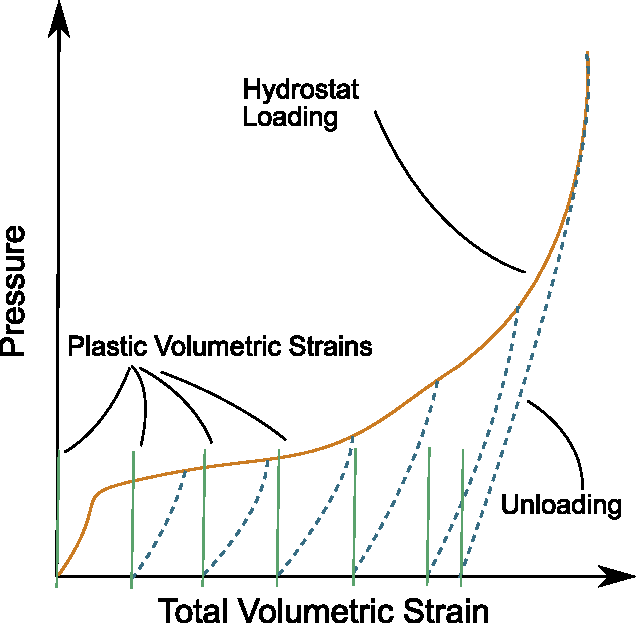
\includegraphics[width=0.5\textwidth]{MPMMaterials/FIGS/TabularHydrostat.pdf}
  \end{center}

  The bulk modulus is determined from a table of unloading curves.  Each unloading 
  curve is associated with a Hencky plastic volumetric strain ($\bar{\Veps_v^p}$).
  These strains are associated in the JSON file with the key \textsf{PlasticStrainVol}
  and added as the first independent variable in the Vaango \textsf{ups} input file.

  For each plastic strain value, the JSON file has to contain an associated data
  set of \textsf{TotalStrainVol} (the total Hencky volumetric strain, $\bar{\Veps_v}$)
  and the \textsf{Pressure} (the mean stress, $\bar{p}$).
\end{SummaryBox}

\begin{SummaryBox}[label=box:TableYieldFunction]{Yield function}
  The tabular yield condition is
  \Beq
     f = \sqrt{J_2} - g(\pbar) = 0
  \Eeq
  \begin{center}
    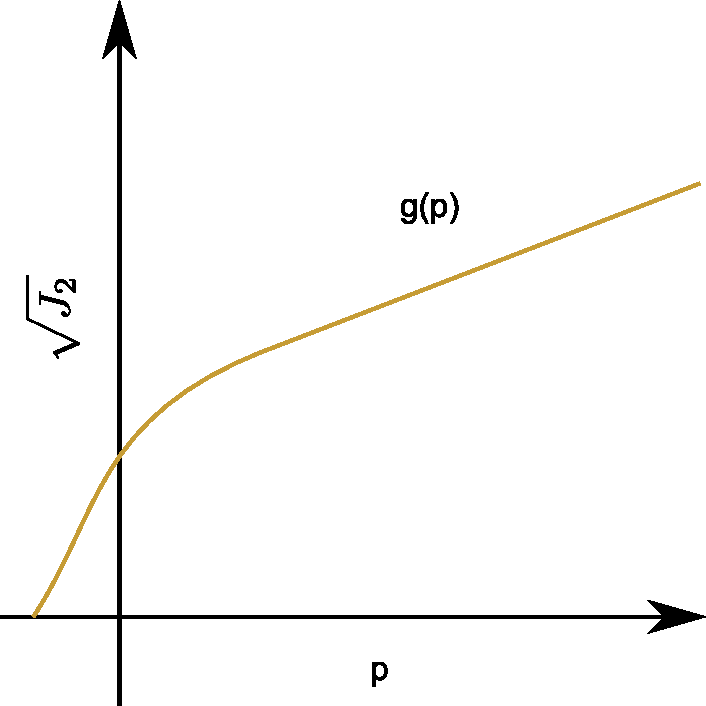
\includegraphics[width=0.4\textwidth]{MPMMaterials/FIGS/TabularYieldFn.pdf}
  \end{center}
  The function $g(\pbar)$ is provided in tabular form.  Only one such function is
  allowed.  The independent variable in the associated JSON file will have the name
  \textsf{Pressure} while the dependent variable will have the name \textsf{SqrtJ2}.
\end{SummaryBox}

\subsection{Examples}
Several examples of input files for exercising various features of the
\Textsfc{TabularPlasticity} model can be found in the directory
\Textsfc{StandAlone/inputs/MPM/TabularModels/TabularPlasticity}.

\subsubsection{von Mises plasticity with linear elasticity compression with rotation}
The input file is \Textsfc{TabularTest\_01\_UniaxialStrainRotateJ2Lin.ups}.
For this problem, $g(\pbar) = \sigma_y$ and $K, G$ are constant. The 
input JSON file for the bulk modulus model is
\begin{lstlisting}[language=JSON]
{"Vaango_tabular_data": {
  "Meta" : {
    "title" : "Test linear elastic data"
  },
  "Data" : {
    "PlasticStrainVol" : [-10.0, 10.0],
    "Data" : [{
      "TotalStrainVol" : [-20.0, 20.0],
      "Pressure" : [-1.0e5,  1.0e5]
    }, {
      "TotalStrainVol" : [-20.0, 20.0],
      "Pressure" : [-1.0e5, 1.0e5]
    }]
  }
}}
\end{lstlisting}
and that for the yield function is
\begin{lstlisting}[language=JSON]
{"Vaango_tabular_data": {
  "Meta" : {
    "title" : "Test von Mises yield data"
  },
  "Data" : {
    "Pressure" : [-0.1e10,  0.1e10],
    "SqrtJ2" :   [  1.0e3,  1.0e3]
  }
}}
\end{lstlisting}
We drive the simulation using uniaxial strain with rotation using the
prescribed deformation file
\begin{lstlisting}[language=sh, backgroundcolor=\color{background}]
0.0   1.000  0.0  0.0   0.0  1.0  0.0   0.0  0.0  1.0    0    0 0 1
1.0   0.900  0.0  0.0   0.0  1.0  0.0   0.0  0.0  1.0   360   0 0 1
\end{lstlisting}
After running the simulation, we get the response shown in Figure~\ref{fig:J2LinRot}.
\begin{figure}[htbp!]
  \begin{subfigure}{0.5\textwidth}
    \centering
    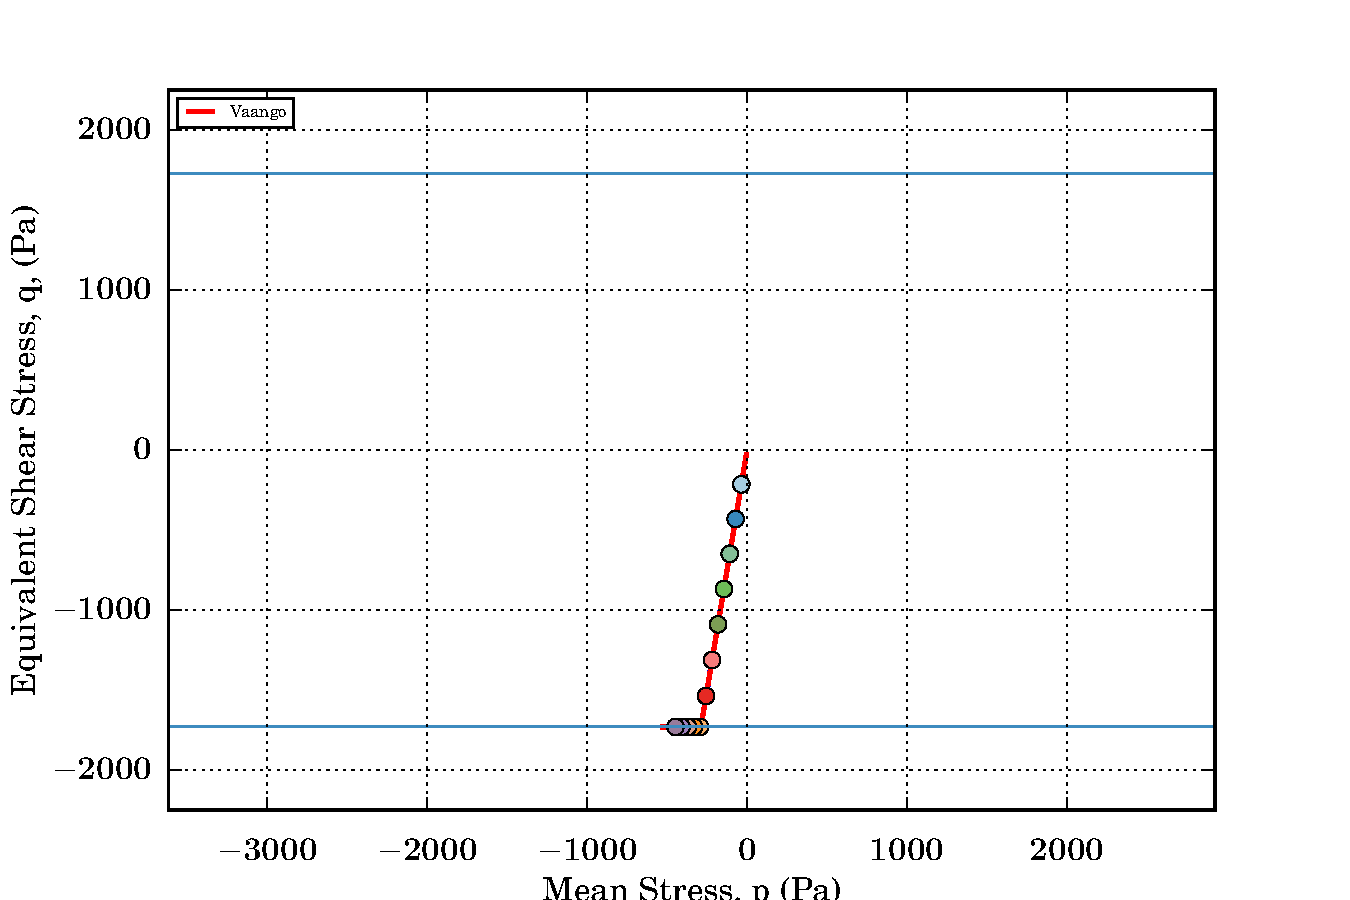
\includegraphics[width=\textwidth]{MPMMaterials/FIGS/UniaxialStrainRotateJ2Lin_yield_surface.pdf}
    \caption{Stress state and yield surface.}
  \end{subfigure}
  \begin{subfigure}{0.5\textwidth}
    \centering
    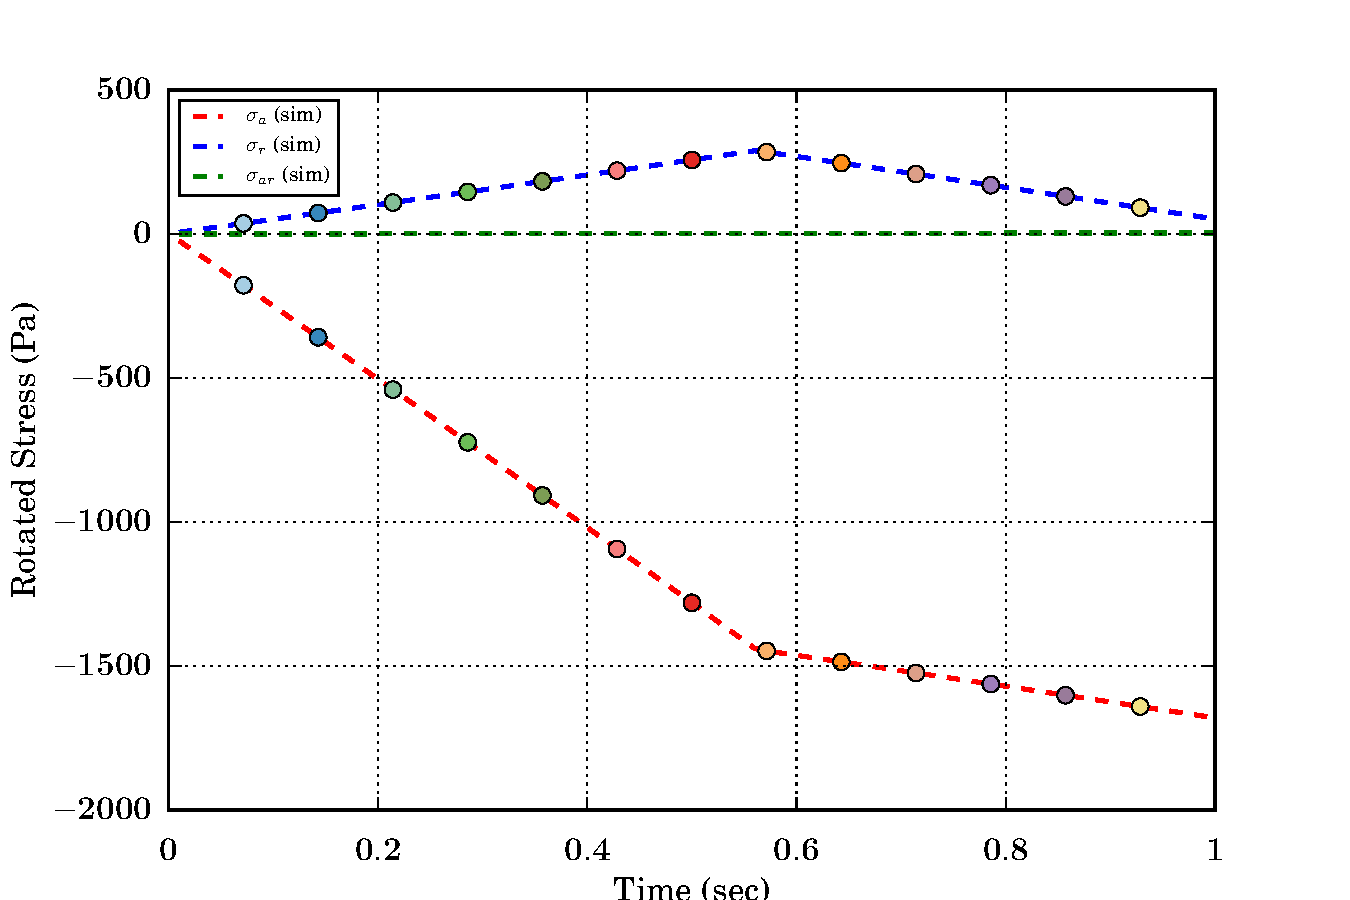
\includegraphics[width=\textwidth]{MPMMaterials/FIGS/UniaxialStrainRotateJ2Lin_sigma_rot_time.pdf}
    \caption{Rotated stress-time curve.}
  \end{subfigure}
  \begin{subfigure}{0.5\textwidth}
    \centering
    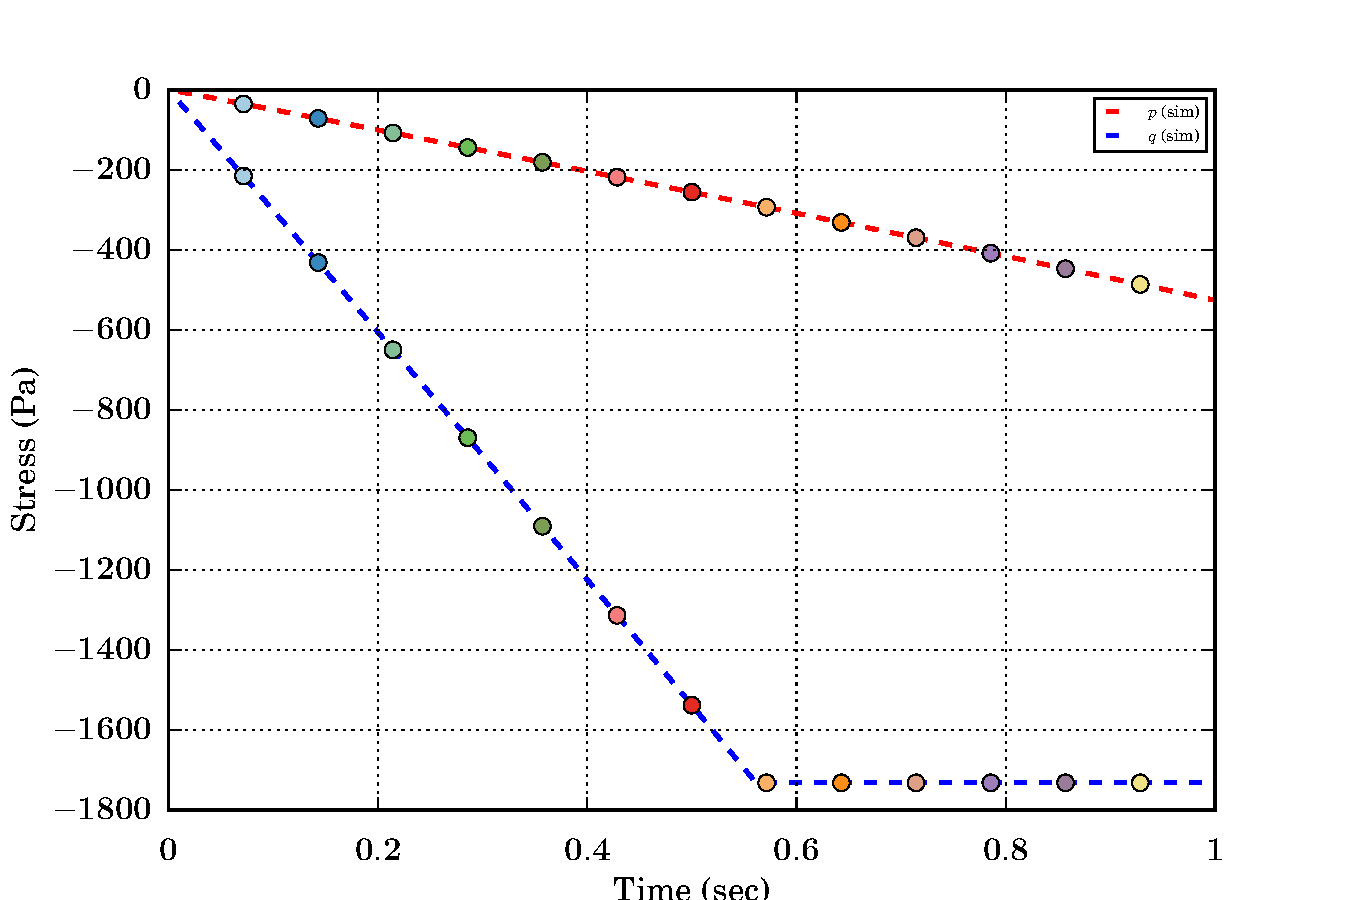
\includegraphics[width=\textwidth]{MPMMaterials/FIGS/UniaxialStrainRotateJ2Lin_pq_time.pdf}
    \caption{Mean and deviatoric stress.}
  \end{subfigure}
  \begin{subfigure}{0.5\textwidth}
    \centering
    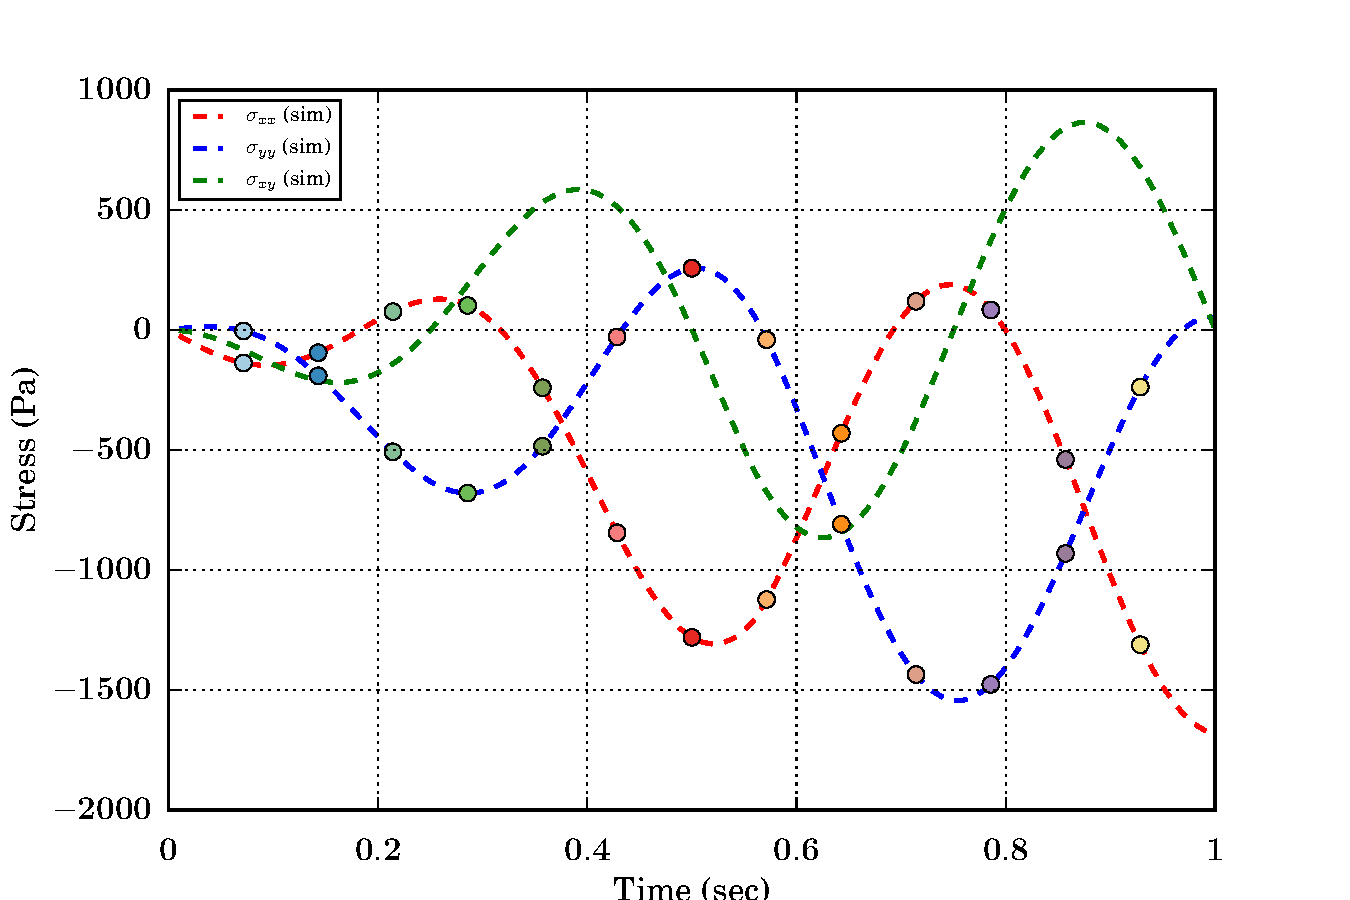
\includegraphics[width=\textwidth]{MPMMaterials/FIGS/UniaxialStrainRotateJ2Lin_sigma_time.pdf}
    \caption{Unrotated stress-time curve.}
  \end{subfigure}
  \caption{Stress evolution for $J_2$ plasticity with linear elasticity under uniaxial
           strain compression with rotation.}
  \label{fig:J2LinRot}
\end{figure}

\newpage
\subsubsection{von Mises plasticity with linear elasticity loading-unloading} 
If we change the prescribed deformation to loading-unloading, using the input 
deformation
\begin{lstlisting}[language=sh, backgroundcolor=\color{background}]
0  1.0  0  0  0  1  0  0  0  1  0  0  0  0
1  1.15  0  0  0  1  0  0  0  1  0  0  0  0
3  1.0  0  0  0  1  0  0  0  1  0  0  0  0
5  0.85  0  0  0  1  0  0  0  1  0  0  0  0
7  1.0  0  0  0  1  0  0  0  1  0  0  0  0
8  1.02 0  0  0  1  0  0  0  1  0  0  0  0
\end{lstlisting}
we get the response shown in Figure~\ref{fig:J2LinLoadUnload}
\begin{figure}[htbp!]
  \begin{subfigure}{0.5\textwidth}
    \centering
    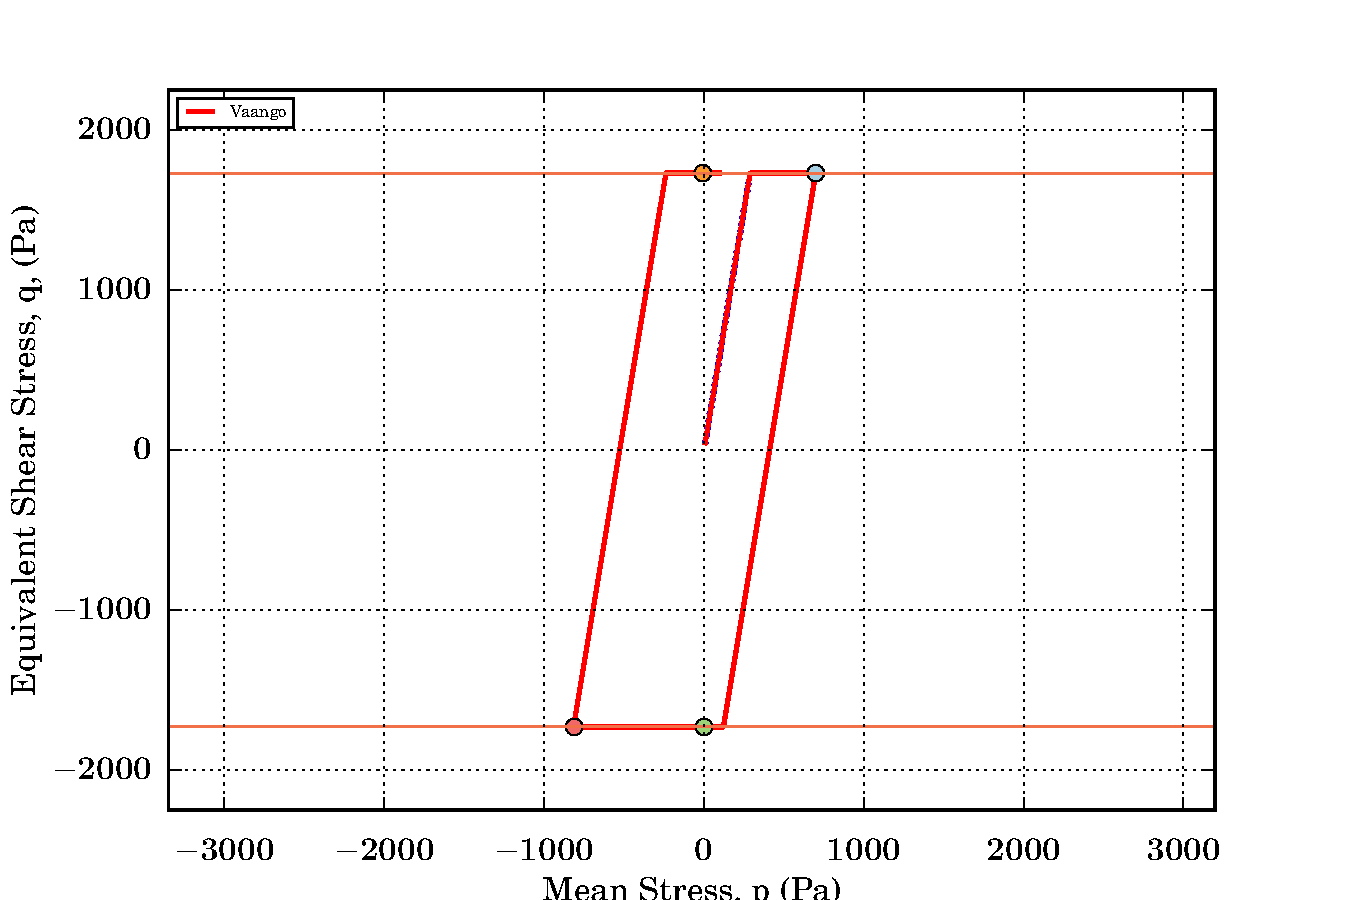
\includegraphics[width=\textwidth]{MPMMaterials/FIGS/UniaxialStrainLoadUnloadJ2Lin_yield_surface.pdf}
    \caption{Stress state and yield surface.}
  \end{subfigure}
  \begin{subfigure}{0.5\textwidth}
    \centering
    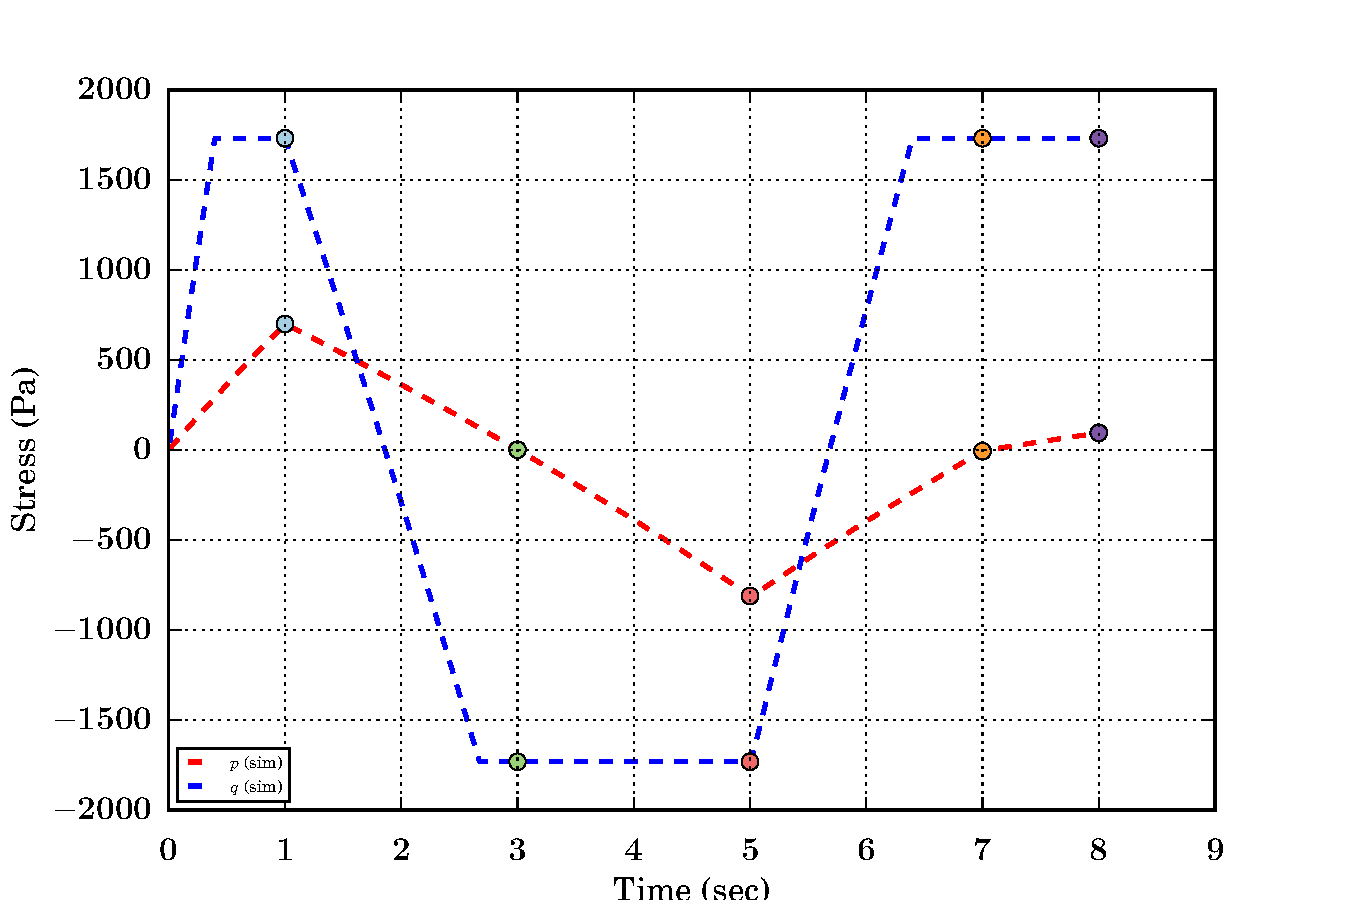
\includegraphics[width=\textwidth]{MPMMaterials/FIGS/UniaxialStrainLoadUnloadJ2Lin_pq_time.pdf}
    \caption{Mean and deviatoric stress vs. time.}
  \end{subfigure}
  \begin{subfigure}{0.5\textwidth}
    \centering
    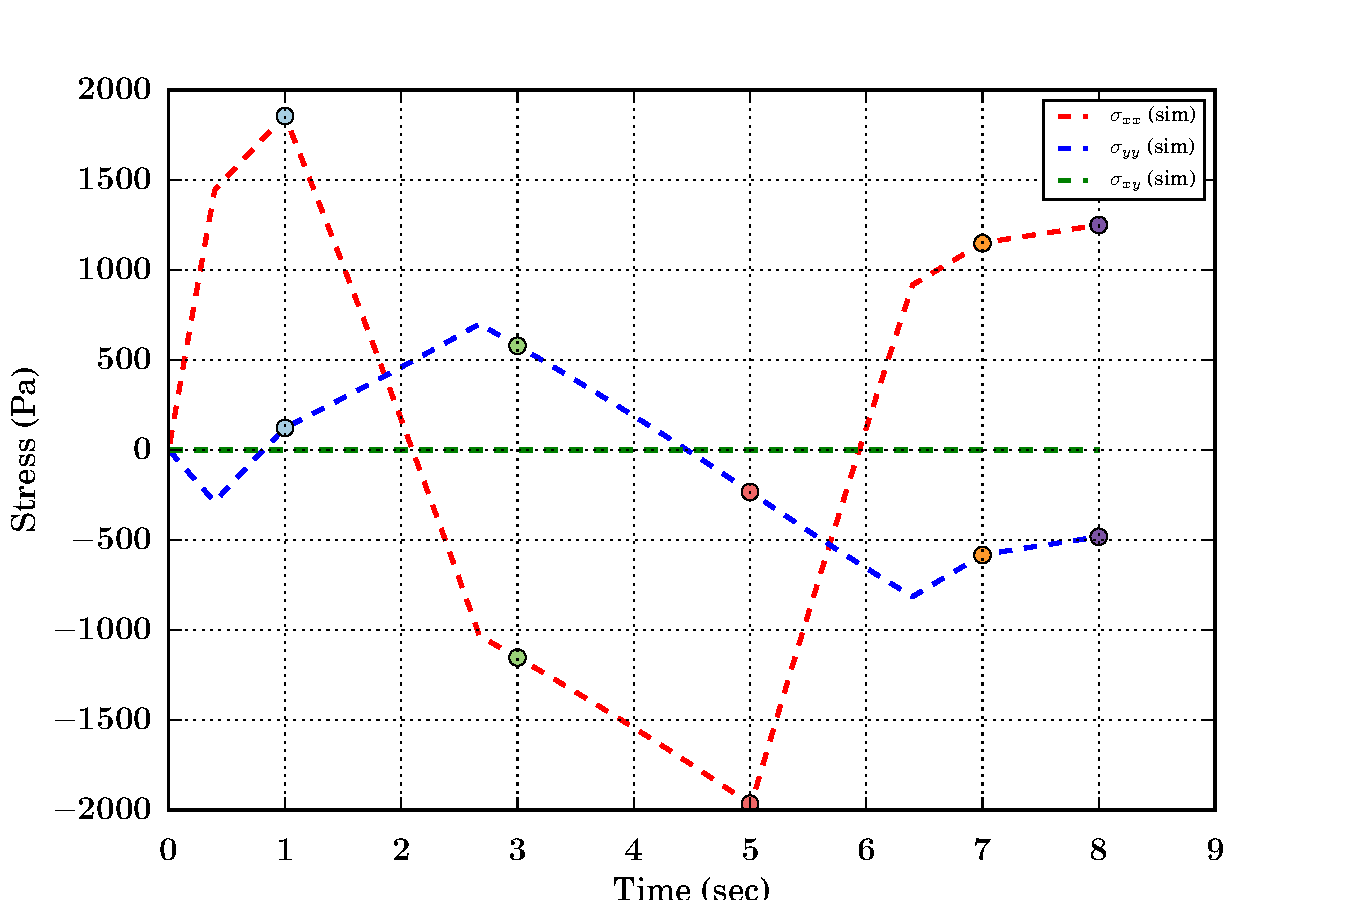
\includegraphics[width=\textwidth]{MPMMaterials/FIGS/UniaxialStrainLoadUnloadJ2Lin_sigma_time.pdf}
    \caption{Stress versus time.}
  \end{subfigure}
  \caption{Stress evolution for $J_2$ plasticity with linear elasticity under uniaxial strain
           loading and unloading.}
  \label{fig:J2LinLoadUnload}
\end{figure}

\newpage
\subsubsection{von Mises plasticity with nonlinear elasticity loading-unloading} 
If we replace the linear elastic model with a nonlinear one:
\begin{lstlisting}[language=JSON]
{"Vaango_tabular_data": {
  "Meta" : {
    "title" : "Test nonlinear elastic data"
  },
  "Data" : {
    "PlasticStrainVol" : [-0.02, 0.02],
    "Data" : [{
      "TotalStrainVol" : [-0.295000, -0.276034, -0.257069, -0.238103, -0.219138, -0.200172, -0.181207, -0.162241, -0.143276, -0.124310, -0.105345, -0.086379, -0.067414, -0.048448, -0.029483, -0.010517, 0.008448,0.027414, 0.046379, 0.065345, 0.084310, 0.103276, 0.122241, 0.141207, 0.160172, 0.179138, 0.198103, 0.217069, 0.236034, 0.255000],
      "Pressure" : [-3000.000000, -2982.413871, -2929.861667, -2842.959514, -2722.726259, -2570.571529, -2388.279197, -2177.986476, -1942.158854, -1683.561196, -1405.225322, -1110.414466, -802.585016, -485.345990, -162.416726, 162.416726, 485.345990, 802.585016, 1110.414466, 1405.225322, 1683.561196, 1942.158854, 2177.986476, 2388.279197, 2570.571529, 2722.726259, 2842.959514, 2929.861667, 2982.413871, 3000.000000]
    }, {
      "TotalStrainVol" : [-0.255000, -0.236034, -0.217069, -0.198103, -0.179138, -0.160172, -0.141207, -0.122241, -0.103276, -0.084310, -0.065345, -0.046379, -0.027414, -0.008448, 0.010517, 0.029483, 0.048448, 0.067414, 0.086379, 0.105345, 0.124310, 0.143276, 0.162241, 0.181207, 0.200172, 0.219138, 0.238103, 0.257069, 0.276034, 0.295000],
      "Pressure" : [-3000.000000, -2982.413871, -2929.861667, -2842.959514, -2722.726259, -2570.571529, -2388.279197, -2177.986476, -1942.158854, -1683.561196, -1405.225322, -1110.414466, -802.585016, -485.345990, -162.416726, 162.416726, 485.345990, 802.585016, 1110.414466, 1405.225322, 1683.561196, 1942.158854, 2177.986476, 2388.279197, 2570.571529, 2722.726259, 2842.959514, 2929.861667, 2982.413871, 3000.000000]
    }]
  }
}}
\end{lstlisting}
we get the response shown in Figure~\ref{fig:J2NonLinLoadUnload}
\begin{figure}[htbp!]
  \begin{subfigure}{0.5\textwidth}
    \centering
    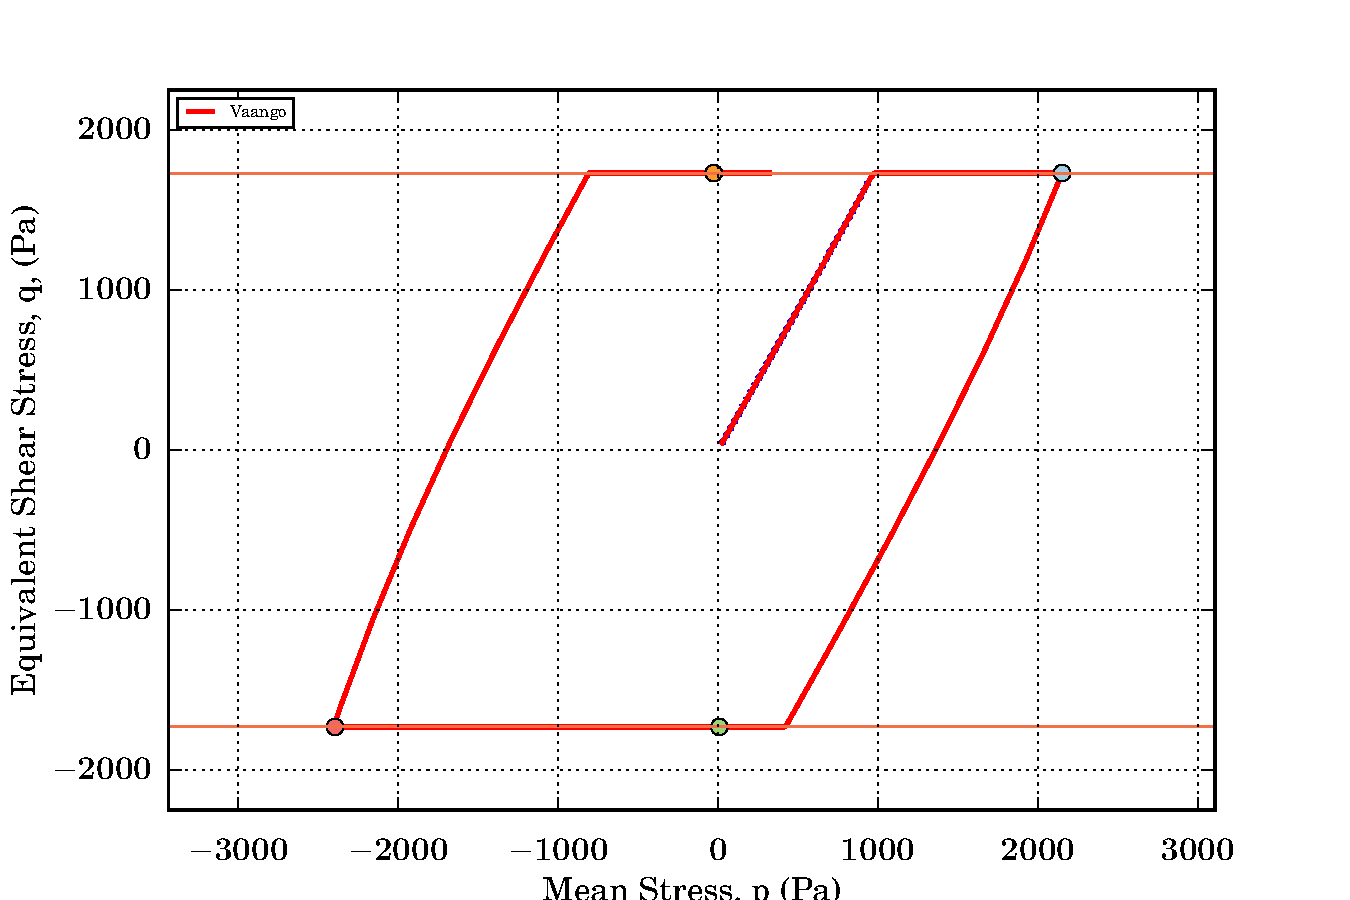
\includegraphics[width=\textwidth]{MPMMaterials/FIGS/UniaxialStrainLoadUnloadJ2NonLin_yield_surface.pdf}
    \caption{Stress state and yield surface.}
  \end{subfigure}
  \begin{subfigure}{0.5\textwidth}
    \centering
    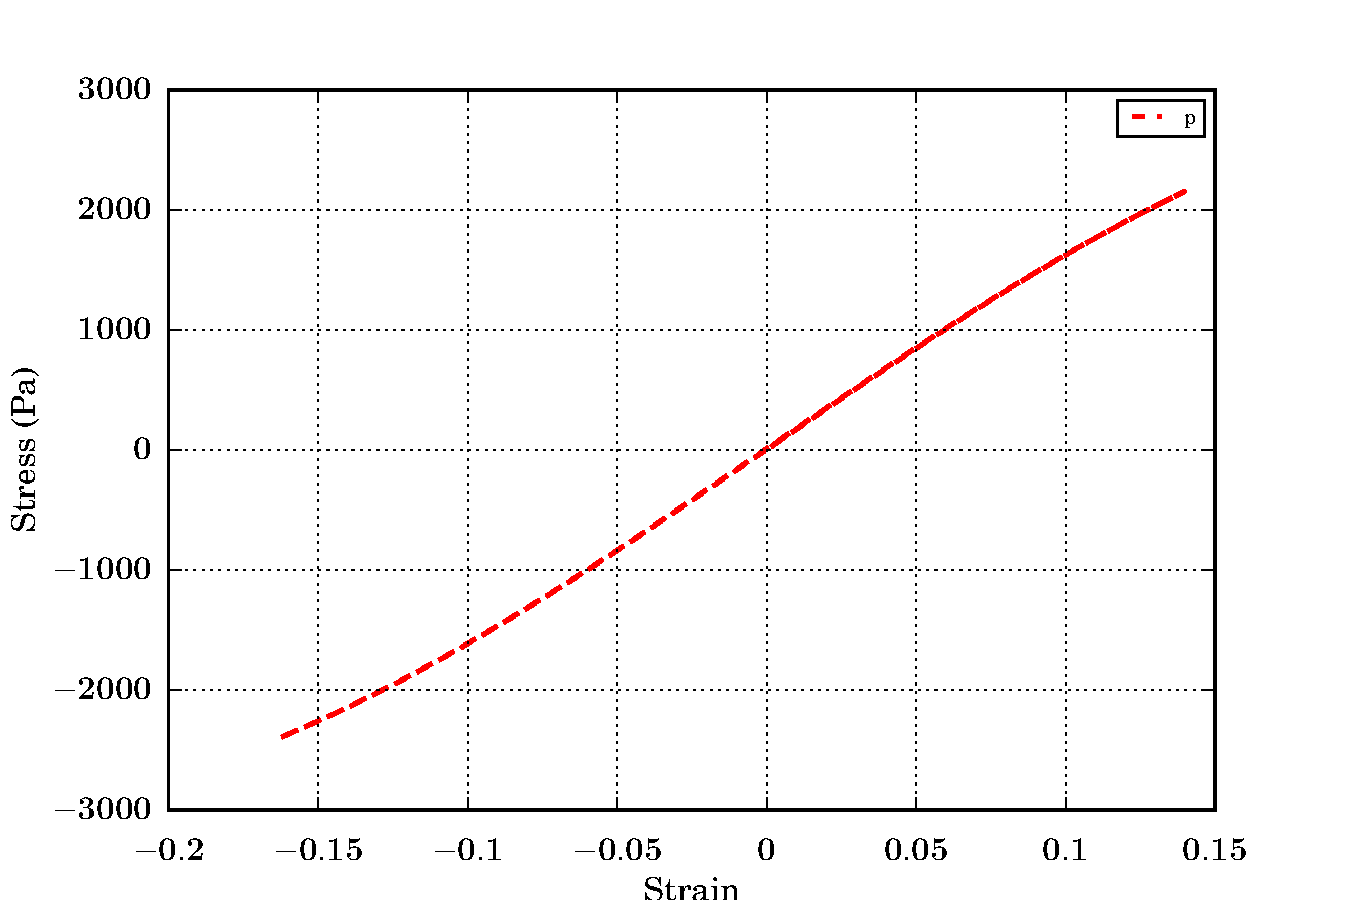
\includegraphics[width=\textwidth]{MPMMaterials/FIGS/UniaxialStrainLoadUnloadJ2NonLin_sigma_eps.pdf}
    \caption{Stress vs. strain.}
  \end{subfigure}
  \begin{subfigure}{0.5\textwidth}
    \centering
    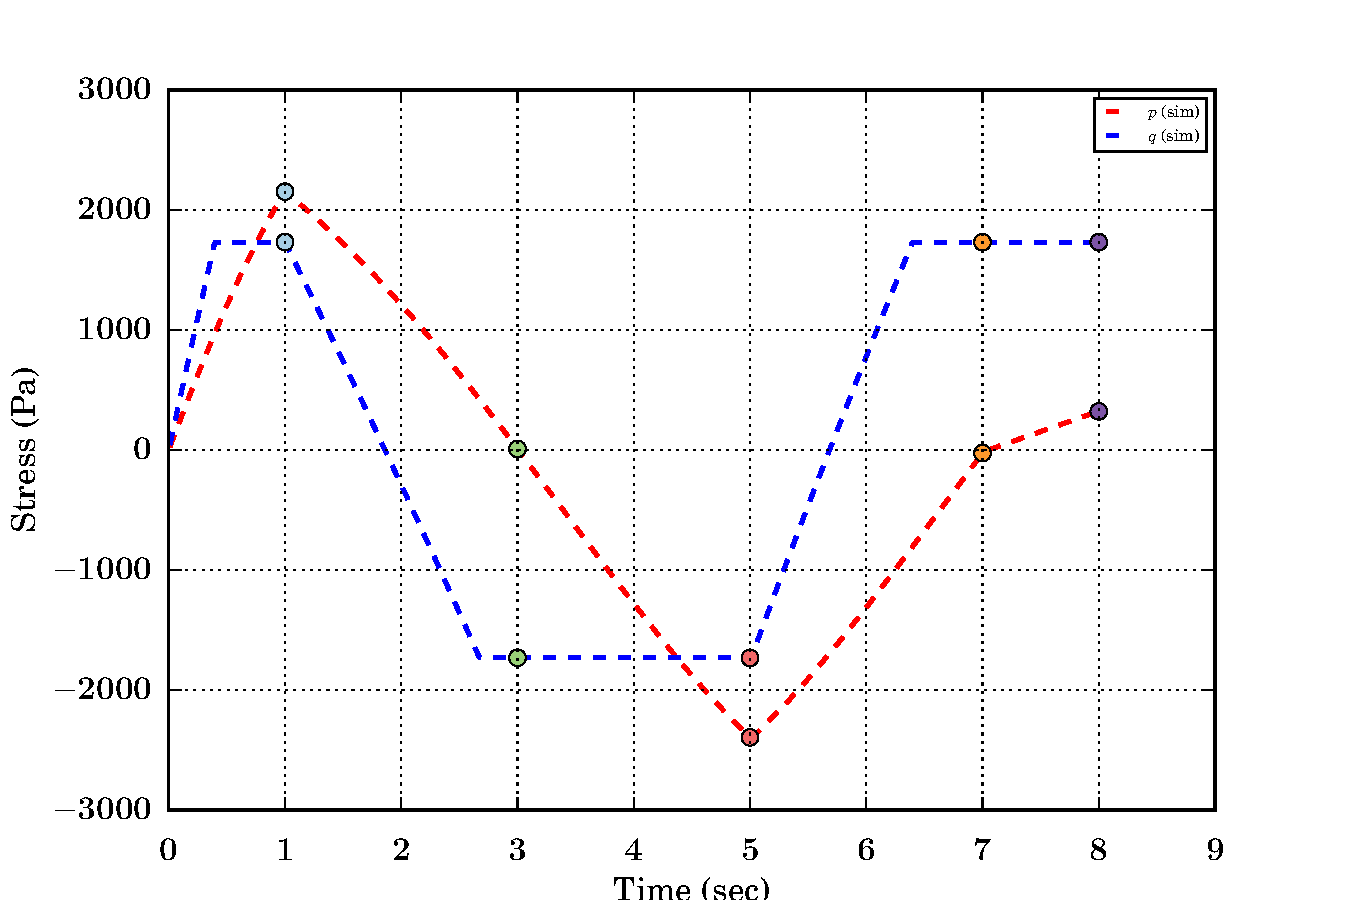
\includegraphics[width=\textwidth]{MPMMaterials/FIGS/UniaxialStrainLoadUnloadJ2NonLin_pq_time.pdf}
    \caption{Mean and deviatoric stress vs. time.}
  \end{subfigure}
  \begin{subfigure}{0.5\textwidth}
    \centering
    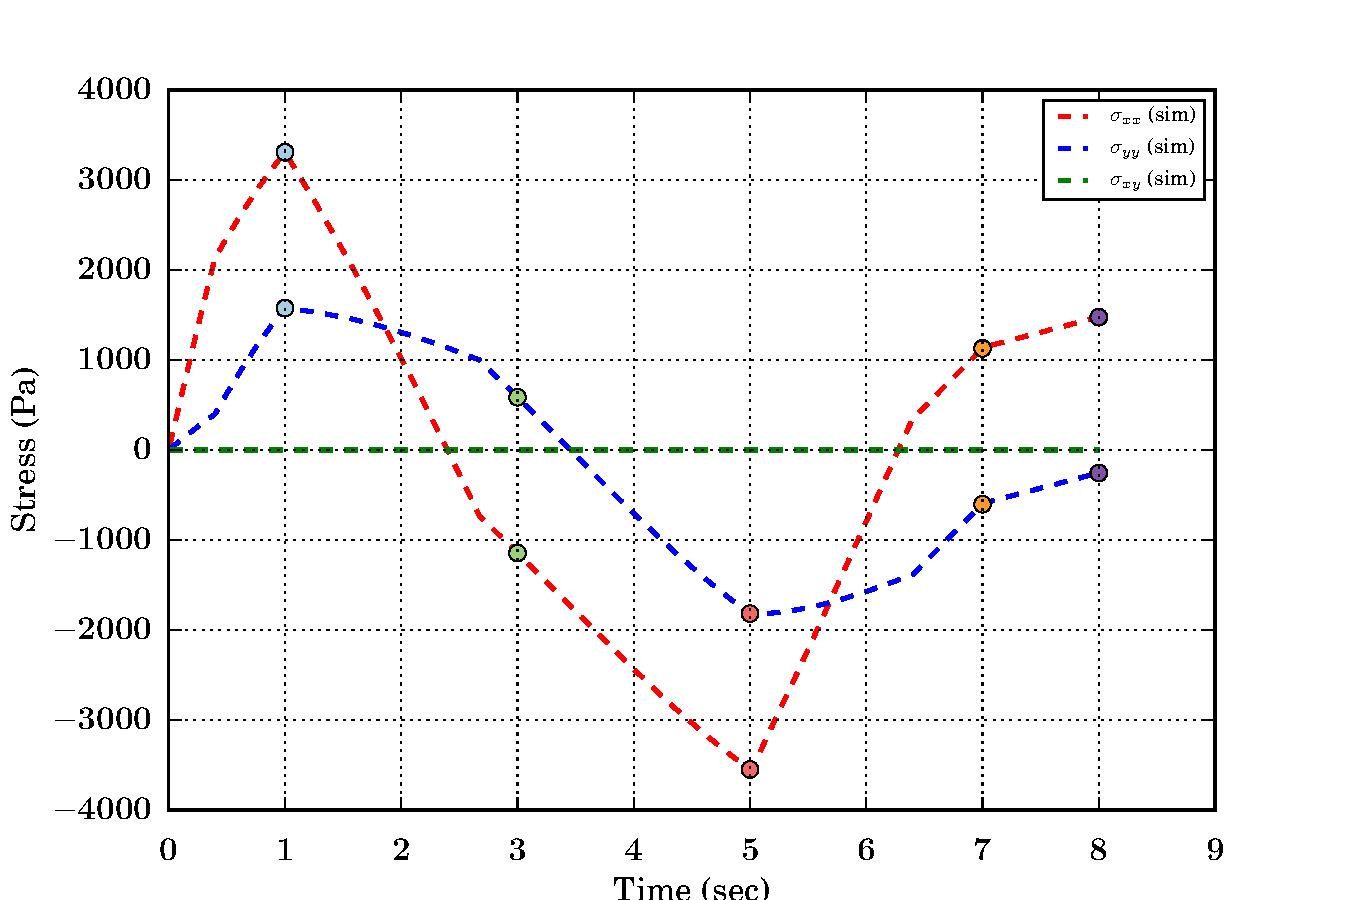
\includegraphics[width=\textwidth]{MPMMaterials/FIGS/UniaxialStrainLoadUnloadJ2NonLin_sigma_time.pdf}
    \caption{Stress versus time.}
  \end{subfigure}
  \caption{Stress evolution for $J_2$ plasticity with nonlinear elasticity under uniaxial strain
           loading and unloading.}
  \label{fig:J2NonLinLoadUnload}
\end{figure}

\newpage
\subsubsection{Linear Drucker-Prager plasticity with nonlinear elasticity loading-unloading} 
If we change the yield function to a linear Drucker-Prager type model:
\begin{lstlisting}[language=JSON]
{"Vaango_tabular_data": {
  "Meta" : {
    "title" : "Test linear Drucker-Prager yield data"
  },
  "Data" : {
    "Pressure" : [-0.1e3,  0.1e10],
    "SqrtJ2" :   [  0,  3.0e8]
  }
}}
\end{lstlisting}
and use the nonlinear elastic model:
\begin{lstlisting}[language=JSON]
{"Vaango_tabular_data": {
  "Meta" : {
    "title" : "Test nonlinear elastic data"
  },
  "Data" : {
    "PlasticStrainVol" : [-2.5, 2.5],
    "Data" : [{
      "TotalStrainVol" : [-15.000000, -14.310345, -13.620690, -12.931034, -12.241379, -11.551724, -10.862069, -10.172414, -9.482759, -8.793103, -8.103448, -7.413793, -6.724138, -6.034483, -5.344828, -4.655172, -3.965517, -3.275862, -2.586207, -1.896552, -1.206897, -0.517241, 0.172414, 0.862069, 1.551724, 2.241379, 2.931034, 3.620690, 4.310345, 5.000000],
      "Pressure" : [-2959.842894, -2943.464146, -2920.494168, -2888.366995, -2843.600634, -2781.548344, -2696.156593, -2579.811517, -2423.426002, -2217.004505, -1950.975669, -1618.496214, -1218.556435, -759.014896, -257.981931, 257.981931, 759.014896, 1218.556435, 1618.496214, 1950.975669, 2217.004505, 2423.426002, 2579.811517, 2696.156593, 2781.548344, 2843.600634, 2888.366995, 2920.494168, 2943.464146, 2959.842894]
    }, {
      "TotalStrainVol" : [-5.000000, -4.310345, -3.620690, -2.931034, -2.241379, -1.551724, -0.862069, -0.172414, 0.517241, 1.206897, 1.896552, 2.586207, 3.275862, 3.965517, 4.655172, 5.344828, 6.034483, 6.724138, 7.413793, 8.103448, 8.793103, 9.482759, 10.172414, 10.862069, 11.551724, 12.241379, 12.931034, 13.620690, 14.310345, 15.000000],
      "Pressure" : [-2959.842894, -2943.464146, -2920.494168, -2888.366995, -2843.600634, -2781.548344, -2696.156593, -2579.811517, -2423.426002, -2217.004505, -1950.975669, -1618.496214, -1218.556435, -759.014896, -257.981931, 257.981931, 759.014896, 1218.556435, 1618.496214, 1950.975669, 2217.004505, 2423.426002, 2579.811517, 2696.156593, 2781.548344, 2843.600634, 2888.366995, 2920.494168, 2943.464146, 2959.842894]
    }]
  }
}}
\end{lstlisting}
we get the response shown in Figure~\ref{fig:DPNonLinLoadUnload}
\begin{figure}[htbp!]
  \begin{subfigure}{0.5\textwidth}
    \centering
    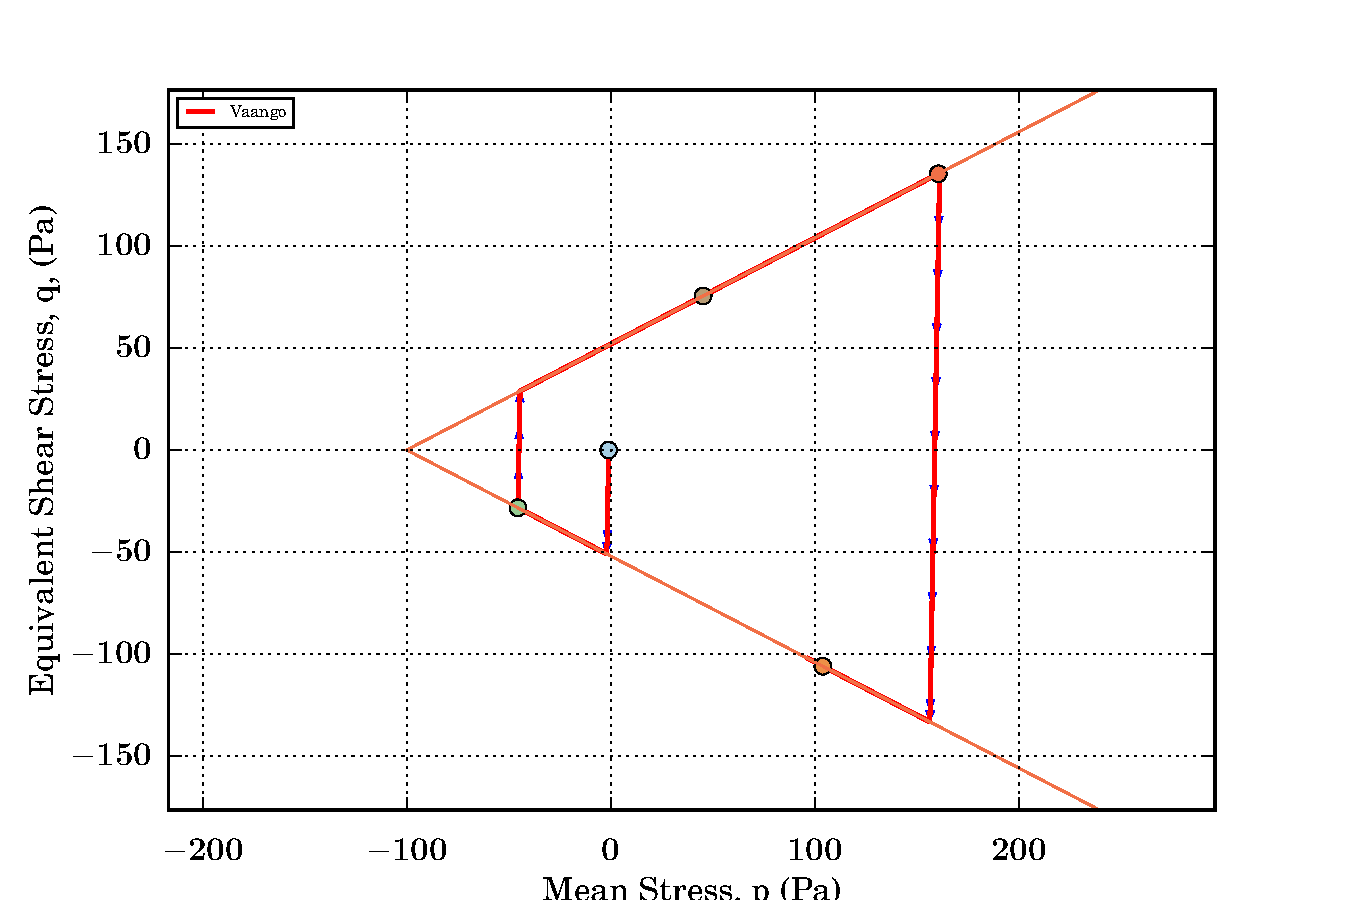
\includegraphics[width=\textwidth]{MPMMaterials/FIGS/UniaxialStrainLoadUnloadDPNonLin_yield_surface.pdf}
    \caption{Stress state and yield surface.}
  \end{subfigure}
  \begin{subfigure}{0.5\textwidth}
    \centering
    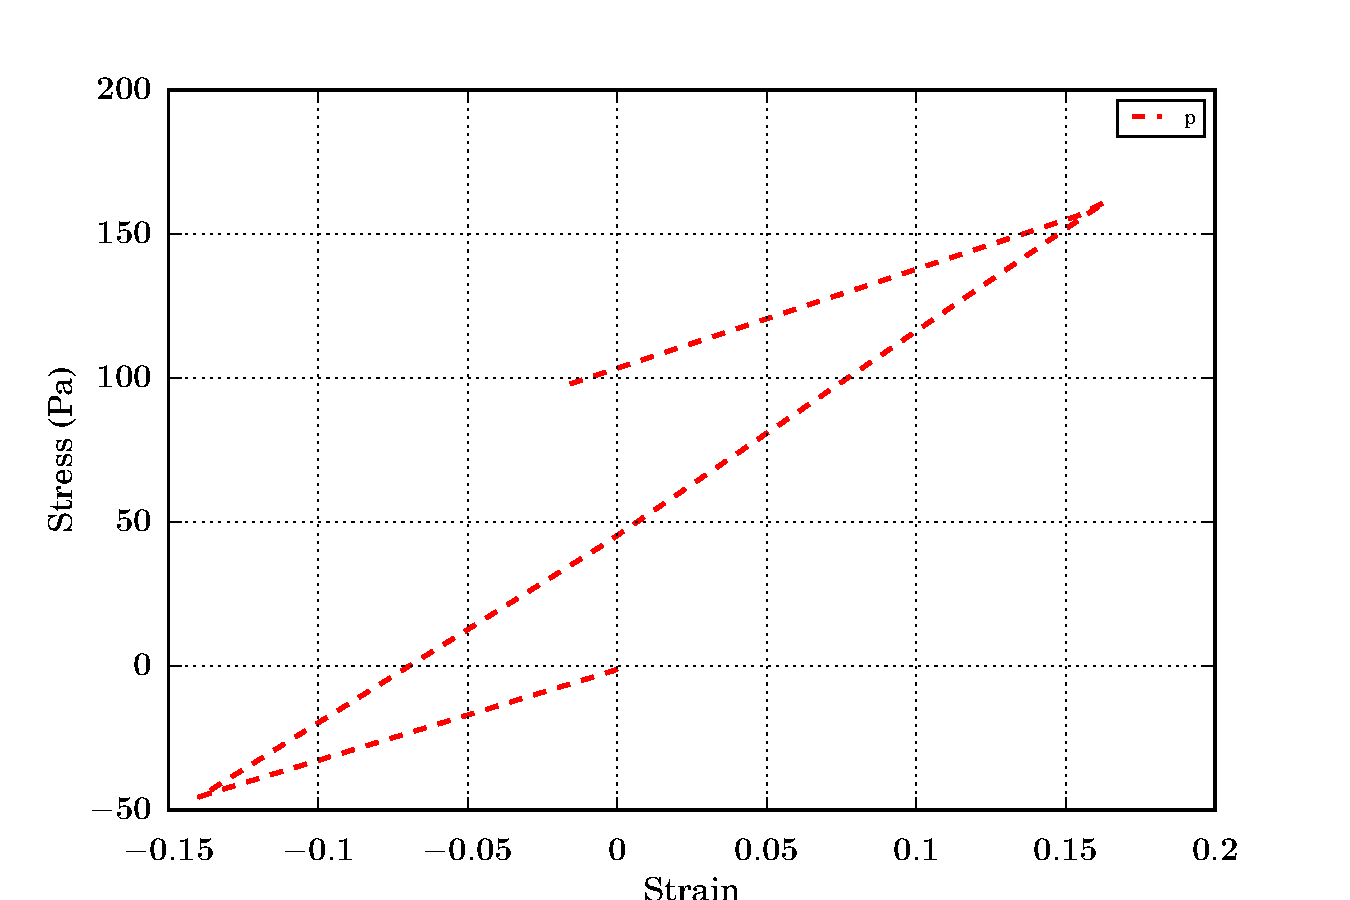
\includegraphics[width=\textwidth]{MPMMaterials/FIGS/UniaxialStrainLoadUnloadDPNonLin_sigma_eps.pdf}
    \caption{Stress vs. strain.}
  \end{subfigure}
  \begin{subfigure}{0.5\textwidth}
    \centering
    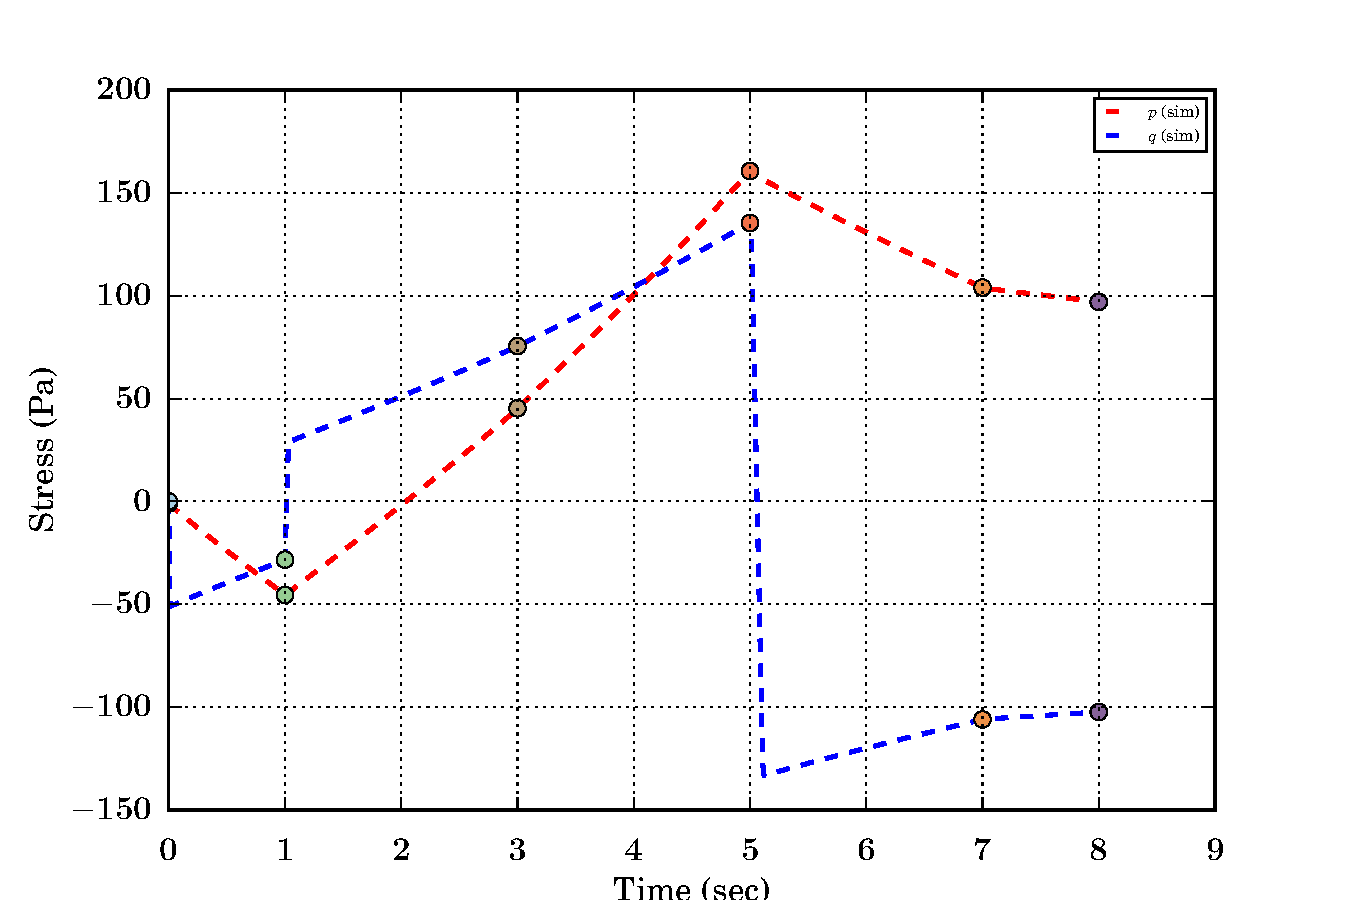
\includegraphics[width=\textwidth]{MPMMaterials/FIGS/UniaxialStrainLoadUnloadDPNonLin_pq_time.pdf}
    \caption{Mean and deviatoric stress vs. time.}
  \end{subfigure}
  \begin{subfigure}{0.5\textwidth}
    \centering
    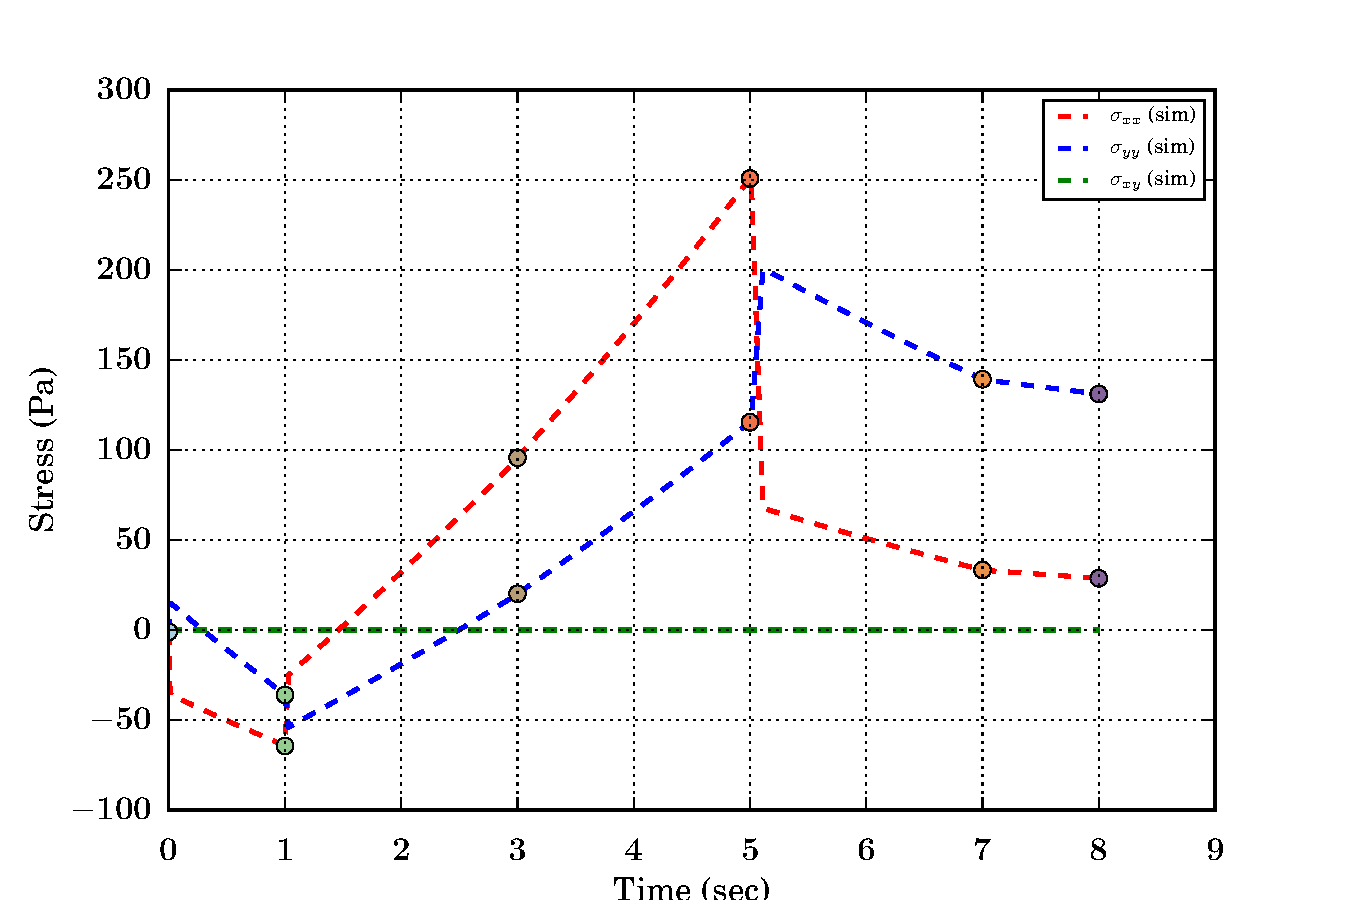
\includegraphics[width=\textwidth]{MPMMaterials/FIGS/UniaxialStrainLoadUnloadDPNonLin_sigma_time.pdf}
    \caption{Stress versus time.}
  \end{subfigure}
  \caption{Stress evolution for Drucker-Prager plasticity with nonlinear elasticity under uniaxial strain
           loading and unloading.}
  \label{fig:DPNonLinLoadUnload}
\end{figure}

\newpage
\subsubsection{Nonlinear Drucker-Prager plasticity with nonlinear elasticity loading-unloading} 
Finally, if we change the yield function to a nonlinear Drucker-Prager type model:
\begin{lstlisting}[language=JSON]
{"Vaango_tabular_data": {
  "Meta" : {
    "title" : "Test nonlinear Drucker-Prager yield data"
  },
  "Data" : {
    "Pressure" : [-333.333333, -298.850575, -264.367816, -229.885057, -195.402299, -160.919540, -126.436782, -91.954023, -57.471264, -22.988506, 11.494253, 45.977011, 80.459770, 114.942529, 149.425287, 183.908046, 218.390805, 252.873563, 287.356322, 321.839080, 356.321839, 390.804598, 425.287356, 459.770115, 494.252874, 528.735632, 563.218391, 597.701149, 632.183908, 666.666667],
    "SqrtJ2" :   [0.000000, 45.485883, 64.326752, 78.783860, 90.971765, 101.709526, 111.417203, 120.344334, 128.653504, 136.457648, 143.838990, 150.859606, 157.567719, 164.001682, 170.192589, 176.166066,181.943530, 187.543098, 192.980256, 198.268366, 203.419051, 208.442500, 213.347701, 218.142630, 222.834406, 227.429413, 231.933403, 236.351579, 240.688667, 244.948974]
  }
}}
\end{lstlisting}
we get the response shown in Figure~\ref{fig:NonLinDPNonLinLoadUnload}
\begin{figure}[htbp!]
  \begin{subfigure}{0.5\textwidth}
    \centering
    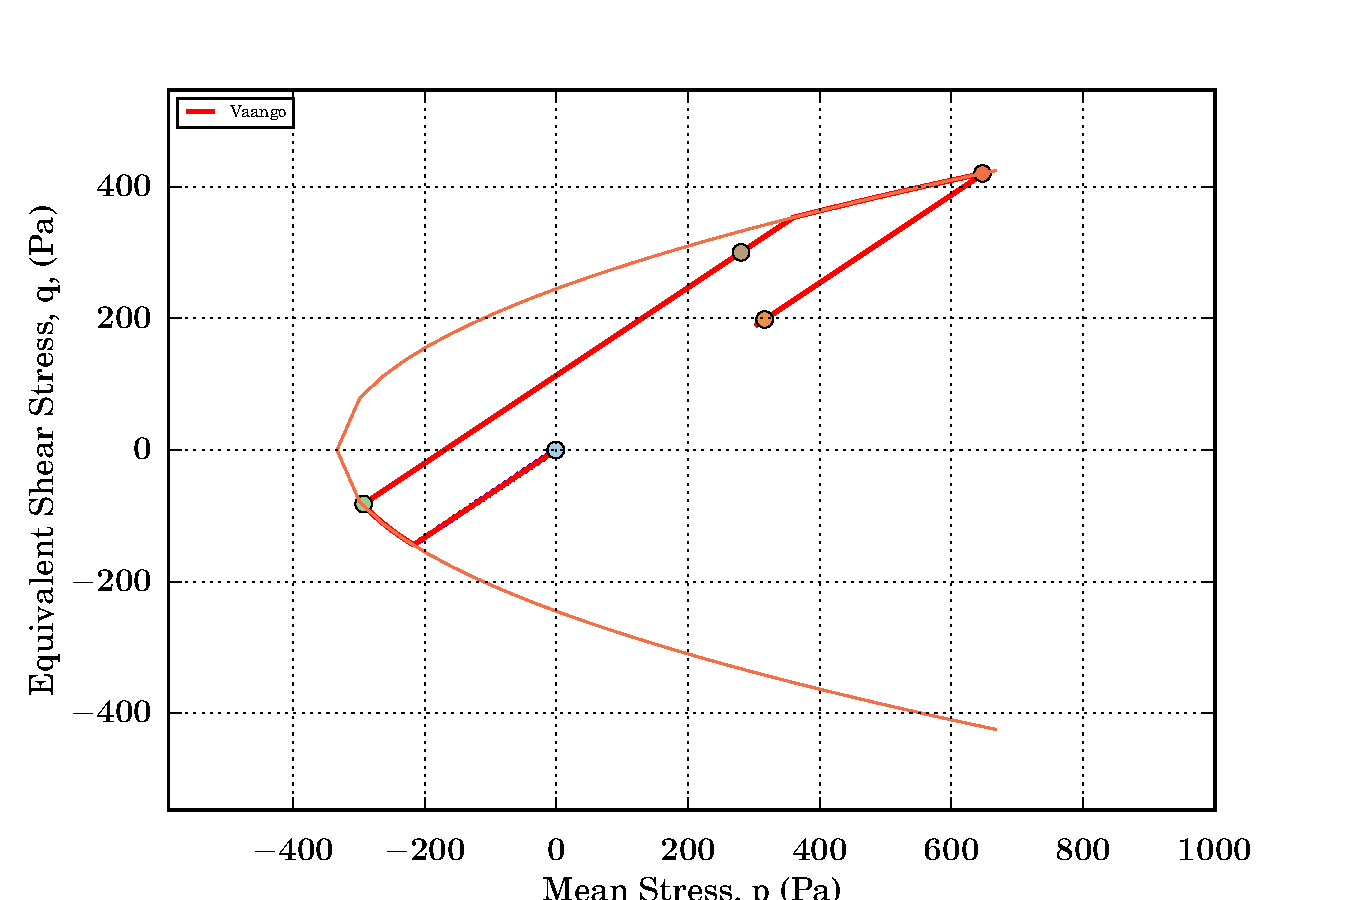
\includegraphics[width=\textwidth]{MPMMaterials/FIGS/UniaxialStrainLoadUnloadNonLinDPNonLin_yield_surface.pdf}
    \caption{Stress state and yield surface.}
  \end{subfigure}
  \begin{subfigure}{0.5\textwidth}
    \centering
    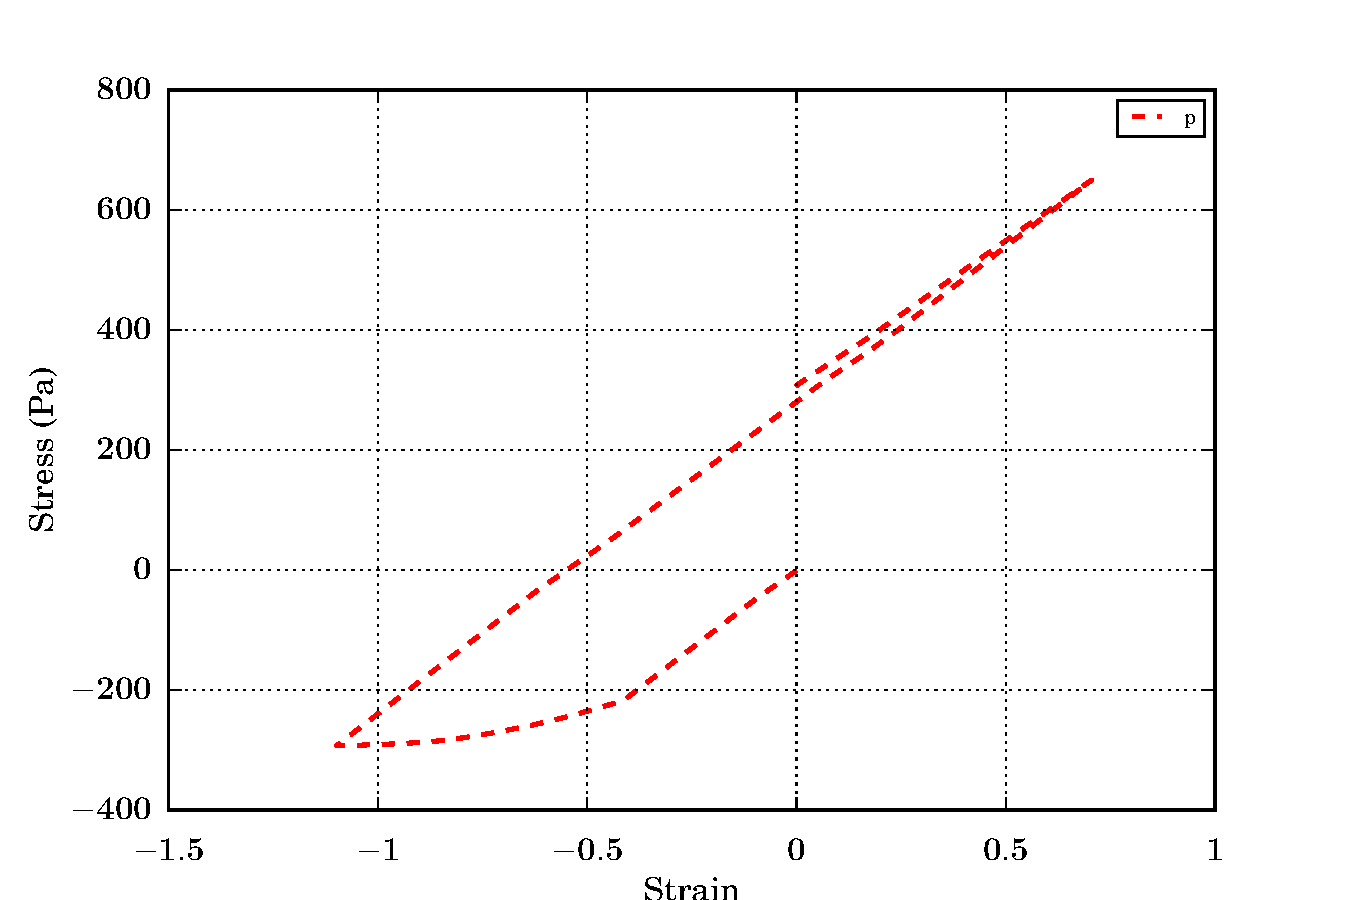
\includegraphics[width=\textwidth]{MPMMaterials/FIGS/UniaxialStrainLoadUnloadNonLinDPNonLin_sigma_eps.pdf}
    \caption{Stress vs. strain.}
  \end{subfigure}
  \begin{subfigure}{0.5\textwidth}
    \centering
    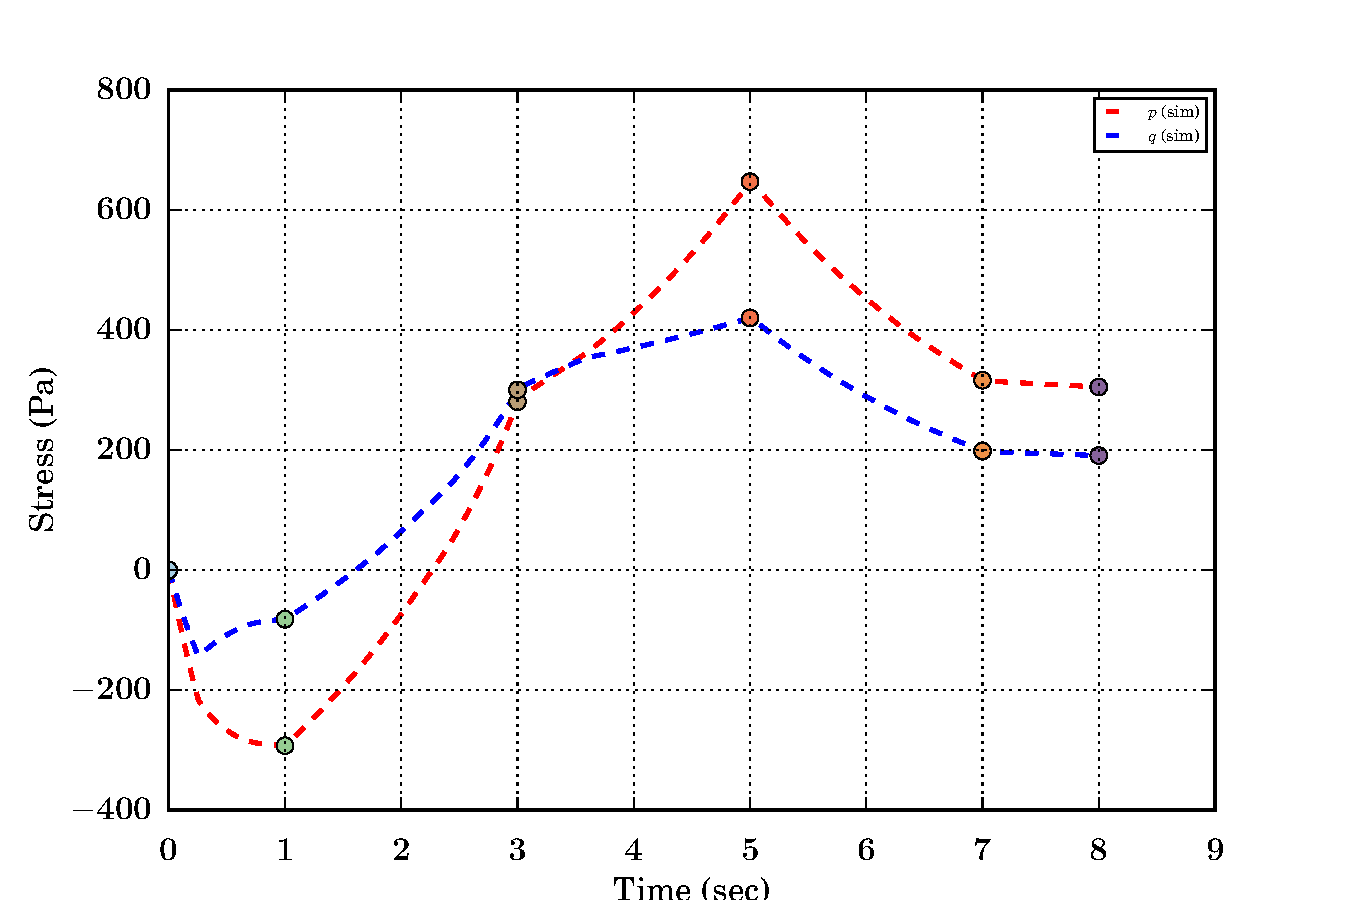
\includegraphics[width=\textwidth]{MPMMaterials/FIGS/UniaxialStrainLoadUnloadNonLinDPNonLin_pq_time.pdf}
    \caption{Mean and deviatoric stress vs. time.}
  \end{subfigure}
  \begin{subfigure}{0.5\textwidth}
    \centering
    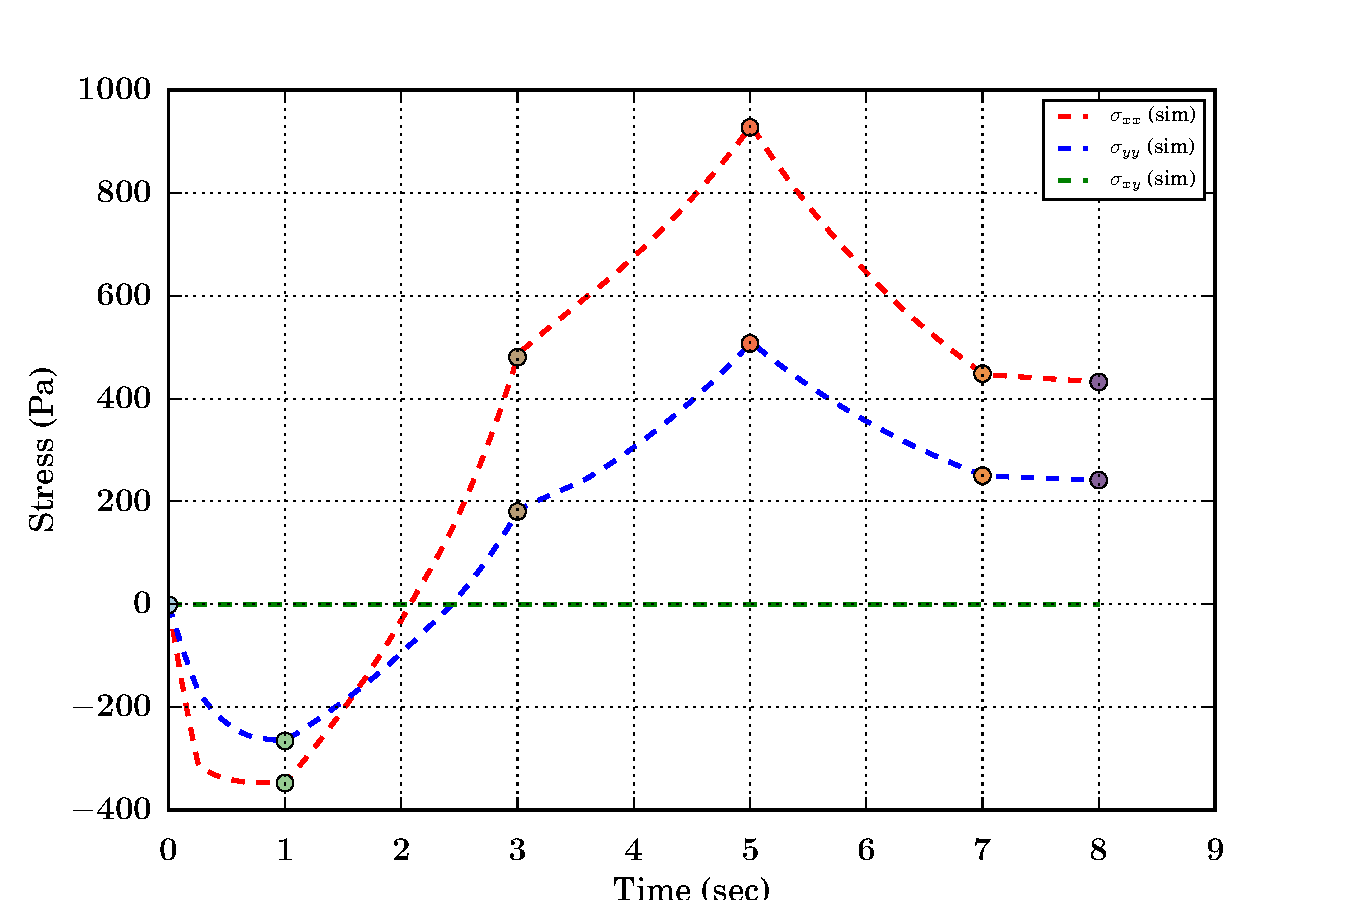
\includegraphics[width=\textwidth]{MPMMaterials/FIGS/UniaxialStrainLoadUnloadNonLinDPNonLin_sigma_time.pdf}
    \caption{Stress versus time.}
  \end{subfigure}
  \caption{Stress evolution for Drucker-Prager plasticity with nonlinear elasticity under uniaxial strain
           loading and unloading.}
  \label{fig:NonLinDPNonLinLoadUnload}
\end{figure}

\subsection{Python script for converting CSV to JSON} \label{app:tabular_elastic_py}
A JSON format is used for the input data in tabular models.  The python script below shows an example
that can be modified for converting data into the \Textsfc{JSON} format used
by \Vaango.  If the input data are in an Excel spreadsheet, they have to be saved as CSV
(comma separated values) before they can be translated into JSON.
\begin{lstlisting}[language=Python]
#  Compression is positive
import numpy as np
import pandas as pd
import matplotlib.pyplot as plt
import json
import PolylineIntersection as pl
import imp
pl = imp.reload(pl)

# Load the CSV data into Pandas dataframes
hydrostat = pd.read_csv("./DrySand_Hydrostat.csv", header=0, skiprows=7)
data_09 = pd.read_csv("./DrySand_LoadUnload_09.csv", header=0, skiprows=4)
data_18 = pd.read_csv("./DrySand_LoadUnload_18.csv", header=0, skiprows=4)
data_27 = pd.read_csv("./DrySand_LoadUnload_27.csv", header=0, skiprows=4)
data_36 = pd.read_csv("./DrySand_LoadUnload_36.csv", header=0, skiprows=4)
data_45 = pd.read_csv("./DrySand_LoadUnload_45.csv", header=0, skiprows=4)

# Rename the columns of each dataframe
column_names = ["TotalStrainVol", "Pressure", "", "", "", ""]
hydrostat.columns = column_names
data_09.columns = column_names
data_18.columns = column_names
data_27.columns = column_names
data_36.columns = column_names
data_45.columns = column_names

# Convert percent into strain, MPa to Pa
strain_fac = 0.01
pressure_fac = 1.0e6
hydrostat.TotalStrainVol *= strain_fac
hydrostat.Pressure *= pressure_fac
data_09.TotalStrainVol *= strain_fac
data_09.Pressure *= pressure_fac
data_18.TotalStrainVol *= strain_fac
data_18.Pressure *= pressure_fac
data_27.TotalStrainVol *= strain_fac
data_27.Pressure *= pressure_fac
data_36.TotalStrainVol *= strain_fac
data_36.Pressure *= pressure_fac
data_45.TotalStrainVol *= strain_fac
data_45.Pressure *= pressure_fac

# Find the point at which unloading begins
p_max_09 = max(data_09.Pressure)
p_max_index_09 = data_09.Pressure.values.tolist().index(p_max_09)
p_max_18 = max(data_18.Pressure)
p_max_index_18 = data_18.Pressure.values.tolist().index(p_max_18)
p_max_27 = max(data_27.Pressure)
p_max_index_27 = data_27.Pressure.values.tolist().index(p_max_27)
p_max_36 = max(data_36.Pressure)
p_max_index_36 = data_36.Pressure.values.tolist().index(p_max_36)
p_max_45 = max(data_45.Pressure)
p_max_index_45 = data_45.Pressure.values.tolist().index(p_max_45)
p_max_index_00 = (np.abs(p_max_09 - hydrostat.Pressure.values)).argmin()
p_max_00 = hydrostat.Pressure.values[p_max_index_00]

# Create separate dataframes for the unload data
data_09_unload = data_09[p_max_index_09:].copy()
data_18_unload = data_18[p_max_index_18:].copy()
data_27_unload = data_27[p_max_index_27:].copy()
data_36_unload = data_36[p_max_index_36:].copy()
data_45_unload = data_45[p_max_index_45:].copy()

# Find plastic strains by intersecting the unload data with the pressure axis
pressure_axis = ((-1, 0),(1, 0))
poly_09_unload = list(data_09_unload[['TotalStrainVol', 'Pressure']].apply(tuple, axis=1))
line_09_unload = (poly_09_unload[-1], poly_09_unload[-2])
plastic_strain_09 = pl.line_intersection(pressure_axis, line_09_unload)[0]
poly_18_unload = list(data_18_unload[['TotalStrainVol', 'Pressure']].apply(tuple, axis=1))
line_18_unload = (poly_18_unload[-1], poly_18_unload[-2])
plastic_strain_18 = pl.line_intersection(pressure_axis, line_18_unload)[0]
poly_27_unload = list(data_27_unload[['TotalStrainVol', 'Pressure']].apply(tuple, axis=1))
line_27_unload = (poly_27_unload[-1], poly_27_unload[-2])
plastic_strain_27 = pl.line_intersection(pressure_axis, line_27_unload)[0]
poly_36_unload = list(data_36_unload[['TotalStrainVol', 'Pressure']].apply(tuple, axis=1))
line_36_unload = (poly_36_unload[-1], poly_36_unload[-2])
plastic_strain_36 = pl.line_intersection(pressure_axis, line_36_unload)[0]
poly_45_unload = list(data_45_unload[['TotalStrainVol', 'Pressure']].apply(tuple, axis=1))
line_45_unload = (poly_45_unload[-1], poly_45_unload[-2])
plastic_strain_45 = pl.line_intersection(pressure_axis, line_45_unload)[0]

# Compute the volumetric elastic strains by subtracting plastic strains from total strains
data_09_unload.TotalStrainVol -= plastic_strain_09
data_18_unload.TotalStrainVol -= plastic_strain_18
data_27_unload.TotalStrainVol -= plastic_strain_27
data_36_unload.TotalStrainVol -= plastic_strain_36
data_45_unload.TotalStrainVol -= plastic_strain_45

# Reverse the order of the unload data to create elastic loading curves
data_00_load = hydrostat[:p_max_index_00]
data_09_load = data_09_unload.sort_index(ascending=False)
data_18_load = data_18_unload.sort_index(ascending=False)
data_27_load = data_27_unload.sort_index(ascending=False)
data_36_load = data_36_unload.sort_index(ascending=False)
data_45_load = data_45_unload.sort_index(ascending=False)

# Simplify the loading dataframes and remove duplicates (if any)
data_00_all = data_00_load[['TotalStrainVol', 'Pressure']].copy().drop_duplicates()
data_09_all = data_09_load[['TotalStrainVol', 'Pressure']].copy().drop_duplicates()
data_18_all = data_18_load[['TotalStrainVol', 'Pressure']].copy().drop_duplicates()
data_27_all = data_27_load[['TotalStrainVol', 'Pressure']].copy().drop_duplicates()
data_36_all = data_36_load[['TotalStrainVol', 'Pressure']].copy().drop_duplicates()
data_45_all = data_45_load[['TotalStrainVol', 'Pressure']].copy().drop_duplicates()

# Compute the total volumetric strain
data_09_all.TotalStrainVol += plastic_strain_09
data_18_all.TotalStrainVol += plastic_strain_18
data_27_all.TotalStrainVol += plastic_strain_27
data_36_all.TotalStrainVol += plastic_strain_36
data_45_all.TotalStrainVol += plastic_strain_45

# Create an extra data set for tension interpolations
data_09_tension_all = data_00_all.copy()
data_09_tension_all.TotalStrainVol -= plastic_strain_09

# Visual check of data set
fig = plt.figure(figsize=(6,6))
ax = fig.add_subplot(111)
plt.plot(data_09_tension_all.TotalStrainVol, data_09_tension_all.Pressure, 'C7')
plt.plot(data_00_all.TotalStrainVol, data_00_all.Pressure, 'C0')
plt.plot(data_09_all.TotalStrainVol, data_09_all.Pressure, 'C1')
plt.plot(data_18_all.TotalStrainVol, data_18_all.Pressure, 'C2')
plt.plot(data_27_all.TotalStrainVol, data_27_all.Pressure, 'C3')
plt.plot(data_36_all.TotalStrainVol, data_36_all.Pressure, 'C4')
plt.plot(data_45_all.TotalStrainVol, data_45_all.Pressure, 'C5')
plt.grid(True)
plt.axis([-0.1, 0.4, 0, 2e9])
plt.xlabel('Engineering volumetric strain', fontsize=16)
plt.ylabel('Pressure (Pa)', fontsize=16)
fig.savefig('Fox_DrySand_ElasticData.png')

# Create data that can be written as JSON
elastic_data_json_09_t = {}
elastic_data_json_09_t["TotalStrainVol"] = data_09_tension_all.TotalStrainVol.values.tolist()
elastic_data_json_09_t["Pressure"] = data_09_tension_all.Pressure.values.tolist()
#json.dumps(elastic_data_json_09_t)
elastic_data_json_00 = {}
elastic_data_json_00["TotalStrainVol"] = data_00_all.TotalStrainVol.values.tolist()
elastic_data_json_00["Pressure"] = data_00_all.Pressure.values.tolist()
#json.dumps(elastic_data_json_00)
elastic_data_json_09 = {}
elastic_data_json_09["TotalStrainVol"] = data_09_all.TotalStrainVol.values.tolist()
elastic_data_json_09["Pressure"] = data_09_all.Pressure.values.tolist()
#json.dumps(elastic_data_json_09)
elastic_data_json_18 = {}
elastic_data_json_18["TotalStrainVol"] = data_18_all.TotalStrainVol.values.tolist()
elastic_data_json_18["Pressure"] = data_18_all.Pressure.values.tolist()
#json.dumps(elastic_data_json_18)
elastic_data_json_27 = {}
elastic_data_json_27["TotalStrainVol"] = data_27_all.TotalStrainVol.values.tolist()
elastic_data_json_27["Pressure"] = data_27_all.Pressure.values.tolist()
#json.dumps(elastic_data_json_27)
elastic_data_json_36 = {}
elastic_data_json_36["TotalStrainVol"] = data_36_all.TotalStrainVol.values.tolist()
elastic_data_json_36["Pressure"] = data_36_all.Pressure.values.tolist()
#json.dumps(elastic_data_json_36)
elastic_data_json_45 = {}
elastic_data_json_45["TotalStrainVol"] = data_45_all.TotalStrainVol.values.tolist()
elastic_data_json_45["Pressure"] = data_45_all.Pressure.values.tolist()
#json.dumps(elastic_data_json_45)

# Set up plastic strain list
plastic_strain_data = [-plastic_strain_09, 0, plastic_strain_09, plastic_strain_18, plastic_strain_27, plastic_strain_36, plastic_strain_45]

# Set up elastic data list
vaango_elastic_data = {}
vaango_elastic_data["PlasticStrainVol"] = plastic_strain_data
vaango_elastic_data["Data"] = [elastic_data_json_09_t, elastic_data_json_00, elastic_data_json_09, elastic_data_json_18, elastic_data_json_27, elastic_data_json_36, elastic_data_json_45]

# Write JSON
meta_data_json = {}
meta_data_json["title"] = "Dry sand nonlinear elasticity data"

vaango_data = {}
vaango_data["Meta"] = meta_data_json
vaango_data["Data"] = vaango_elastic_data
json.dumps(vaango_data)

vaango_input_data = {}
vaango_input_data["Vaango_tabular_data"] = vaango_data
json.dumps(vaango_input_data, sort_keys=True)

with open('DrySand_ElasticData.json', 'w') as outputFile:
    json.dump(vaango_input_data, outputFile, sort_keys=True, indent=2)
\end{lstlisting}

The above script uses an intersection algorithm called "PolylineIntersection.py" which is listed below.
\begin{lstlisting}[language=Python]
def line_intersection(line1, line2):
    xdiff = (line1[0][0] - line1[1][0], line2[0][0] - line2[1][0])
    ydiff = (line1[0][1] - line1[1][1], line2[0][1] - line2[1][1])

    def det(a, b):
        return a[0] * b[1] - a[1] * b[0]

    div = det(xdiff, ydiff)
    if div == 0:
       return None

    d = (det(*line1), det(*line2))
    x = det(d, xdiff) / div
    y = det(d, ydiff) / div
    return (x, y)

def poly_intersection(poly1, poly2):

    for i, p1_first_point in enumerate(poly1[:-1]):
        p1_second_point = poly1[i + 1]

        for j, p2_first_point in enumerate(poly2[:-1]):
            p2_second_point = poly2[j + 1]

            pt = line_intersection((p1_first_point, p1_second_point), (p2_first_point, p2_second_point))
            t = (p2_second_point[0] - pt[0])/(p2_second_point[0] - p2_first_point[0])
            print(j, p1_first_point, p2_first_point, p2_second_point, pt, t)
            if pt and t >= 0 and t <= 1:
                return [True, pt]

    return False
\end{lstlisting}






%%__________________________________
% new commands for all sections
\newcommand{\Comment}[1]{ \marginpar{{\scriptsize \color{red} #1 }}}
\newcommand{\red}[1]{\color{red} {#1} \color{black}}
\newcommand{\TT}[1]{\tt{#1}\normalfont}

% MPM & ICE
\newcommand{\tn}[1]{\mbox{\ensuremath{\mathbf{#1}}}}
\newcommand{\sig}{\mbox{\boldmath $\sigma \!\!$ \unboldmath}}
\newcommand{\bnabla} {\mbox {\boldmath $\nabla \!\!$ \unboldmath}}
\newcommand{\taubold} {\mbox{\boldmath $\tau \!\!$ \unboldmath}}
\newcommand{\f}{\ensuremath{f^{\theta}_r} }

\newcommand{\Texp}{\rm{exp}}
\newcommand{\Teq}{\rm{eq}}
\newcommand{\Delt}{\ensuremath{\Delta t}}
\newcommand{\Epj}{\ensuremath{\epsilon_{p,j}}}
\newcommand{\Epo}{\ensuremath{\epsilon_{p,0}}}
\newcommand{\lambdadot}{\ensuremath{\dot{\lambda}}}
\def\bfE{{\bf E}}

\newcommand{\hangp}[1]{\makebox[0pt][r]{(}#1\makebox[0pt][l]{)}} % New command to create parentheses around text in tables which take up no horizontal space - this improves column spacing
\newcommand{\hangstar}{\makebox[0pt][l]{*}} % New command to create asterisks in tables which take up no horizontal space - this improves column spacing

\newcommand{\monthyear}{\ifcase\month\or January\or February\or March\or April\or May\or June\or July\or August\or September\or October\or November\or December\fi\space\number\year} % A command to print the current month and year

\newcommand{\blankpage}{\newpage\hbox{}\thispagestyle{empty}\newpage} % Command to insert a blank page

\def\rmd{{\rm d}}
\def\rme{{\rm e}}
\def\rmf{{\rm f}}
\def\rmr{{\rm r}}
\def\rmR{{\rm R}}
\def\rms{{\rm s}}
\def\bfd{{\bf d}}
\def\bfE{{\bf E}}
\def\bfF{{\bf F}}
\def\bff{{\bf f}}
\def\bfg{{\bf g}}
\def\bfI{{\bf I}}
\def\bfj{{\bf j}}
\def\bfm{{\bf m}}
\def\bfr{{\bf r}}
\def\bfx{{\bf x}}
\def\bfu{{\bf u}}
\def\rmg{{\rm g}}
\def\bfa{{\bf a}}
\def\bfG{{\bf G}}
\def\bfv{{\bf v}}
\def\tdot{{\textstyle\cdot}}

\pdfcompresslevel=9
%\raggedright

\definecolor{red}{rgb}{1,0,0}
\definecolor{green}{rgb}{0,1,0}
\definecolor{blue}{rgb}{0,0,1}
\definecolor{Red}{rgb}{0.8666,0.03137,0.02352}
\definecolor{Blue}{rgb}{0.00784,0.67059,0.91764}
\definecolor{Darkgreen}{rgb}{0,0.68235,0}
\definecolor{Green}{rgb}{0,0.8,0}
\definecolor{Bl}{rgb}{0,0.2,0.91764}
\definecolor{Royalblue}{rgb}{0,0.2,0.91764}
\definecolor{Brickred}{rgb}{0.644541,0.164065,0.164065}
\definecolor{Brown}{rgb}{0.6,0.4,0.4}
\definecolor{Orange}{rgb}{1,0.647059,0}
\definecolor{Indigo}{rgb}{0.746105,0,0.996109}
\definecolor{Violet}{rgb}{0.308598,0.183597,0.308598}
\definecolor{Lightgrey}{rgb}{0.762951,0.762951,0.762951}
\definecolor{Darkgrey}{rgb}{0.503548,0.503548,0.503548}
\definecolor{Pink}{rgb}{1,0.6,0.6}
\definecolor{MyLightMagenta}{cmyk}{0.1,0.8,0,0.1}
\definecolor{MyDarkBlue}{rgb}{0,0.08,0.45}

\newcommand{\handout}[3]{
        \begin{center}
         % \copyright 
          Biswajit Banerjee \hspace{4.2in} University of Utah\\
          \vspace{10pt}
          {\Large\bf Waves in Composites and Metamaterials}\\
          \vspace{6pt}
          (Instructor: Prof. G. W. Milton)
        \end{center}
        \vspace{8pt}\noindent
        %\begin{center}
        {\underline{\makebox[7.0in]{\large\bf\noindent
                \makebox[1.5in][l]{#1~~~} \hfill {~~~#2~~~} \hfill
                \makebox[1.5in][r]{~~~#3}}}}
        %\end{center}
        }

\newcommand{\heading}[1]{
        \begin{center}{\large\bf{#1}}\end{center}}

\newcommand{\subheading}[1]{
        \begin{center}{\normalsize\bf{#1}}\end{center}}

\newcommand{\subsubheading}[1]{
        \begin{center}{\small\bf{#1}}\end{center}}

\newcommand{\Heading}[1]{
        \vspace{12pt}\begin{center}{\Large\bf{#1}}\end{center}}

\newcommand{\Subheading}[1]{
        \vspace{8pt}\begin{center}{\large\bf{#1}}\end{center}}

\newcommand{\Red}{\color{Brickred}}
\newcommand{\Blue}{\color{Royalblue}}
\newcommand{\Green}{\color{Darkgreen}}
\newcommand{\Violet}{\color{Violet}}
\newcommand{\That}{\ensuremath{\widehat{T}}}
\newcommand{\Jump}[1]{\ensuremath{\llbracket#1\rrbracket}}
\newcommand{\Blimitx}[1]{\ensuremath{\left[#1\right]_{x_a}^{x_b}}}
\newcommand{\Deriv}[2]{\ensuremath{\cfrac{d#1}{d#2}}}
\newcommand{\MDeriv}[2]{\ensuremath{\cfrac{D#1}{D#2}}}
\newcommand{\DDeriv}[2]{\ensuremath{\cfrac{d^2#1}{d#2^2}}}
\newcommand{\DDDeriv}[2]{\ensuremath{\cfrac{d^3#1}{d#2^3}}}
\newcommand{\DDDDeriv}[2]{\ensuremath{\cfrac{d^4#1}{d#2^4}}}
\newcommand{\Intx}{\ensuremath{\int_{x_a}^{x_b}}}
\newcommand{\IntX}{\ensuremath{\int_{X_a}^{X_b}}}
\newcommand{\Intiso}{\ensuremath{\int_{-1}^{1}}}
\newcommand{\IntOmegaA}{\ensuremath{\int_{\Omega_0}}}
\newcommand{\IntOmega}{\ensuremath{\int_{\Omega}}}
\newcommand{\IntDOmega}{\ensuremath{\int_{\partial\Omega}}}
\newcommand{\IntOmegap}{\ensuremath{\int_{\Omega'}}}
\newcommand{\Norm}[2]{\ensuremath{\left\lVert#1\right\rVert_{#2}}}
\newcommand{\norm}[1]{\ensuremath{\left\lVert#1\right\rVert}}
\newcommand{\Var}[1]{\ensuremath{\delta #1}}
\newcommand{\DelT}{\ensuremath{\Delta t}}
\newcommand{\CalD}{\ensuremath{\mathcal{D}}}
\newcommand{\BCalD}{\ensuremath{\boldsymbol{\CalD}}}
\newcommand{\CalF}{\ensuremath{\mathcal{F}}}
\newcommand{\CalL}{\ensuremath{\mathcal{L}}}
\newcommand{\CalM}{\ensuremath{\mathcal{M}}}
\newcommand{\BCalM}{\ensuremath{\boldsymbol{\CalM}}}
\newcommand{\CalN}{\ensuremath{\mathcal{N}}}
\newcommand{\CalP}{\ensuremath{\mathcal{P}}}
\newcommand{\CalS}{\ensuremath{\mathcal{S}}}
\newcommand{\BCalS}{\ensuremath{\boldsymbol{\CalS}}}
\newcommand{\CalT}{\ensuremath{\mathcal{T}}}
\newcommand{\CalV}{\ensuremath{\mathcal{V}}}
\newcommand{\CalW}{\ensuremath{\mathcal{W}}}
\newcommand{\CalX}{\ensuremath{\mathcal{X}}}
\newcommand{\Comp}[2]{\ensuremath{#1 \circ #2}}
\newcommand{\Map}[3]{\ensuremath{#1 : #2 \rightarrow #3}}
\newcommand{\MapTo}[3]{\ensuremath{#1 : #2 \mapsto #3}}
\newcommand{\Real}[1]{\ensuremath{\mathbb{R}^{#1}}}
\newcommand{\Ve}{\ensuremath{\varepsilon}}
\newcommand{\BHat}[1]{\ensuremath{\widehat{\boldsymbol{#1}}}}
\newcommand{\BTx}{\ensuremath{\tilde{\boldsymbol{x}}}}
\newcommand{\Beh}{\ensuremath{\hat{\boldsymbol{e}}}}
\newcommand{\BHex}{\ensuremath{\hat{\boldsymbol{e}}_1}}
\newcommand{\BHey}{\ensuremath{\hat{\boldsymbol{e}}_2}}
\newcommand{\BHez}{\ensuremath{\hat{\boldsymbol{e}}_3}}
\newcommand{\BHn}[1]{\ensuremath{\hat{\boldsymbol{n}}_{#1}}}
\newcommand{\BHe}[1]{\ensuremath{\hat{\boldsymbol{e}}_{#1}}}
\newcommand{\BHg}[1]{\ensuremath{\hat{\boldsymbol{g}}_{#1}}}
\newcommand{\BHG}[1]{\ensuremath{\hat{\boldsymbol{G}}_{#1}}}
\newcommand{\Hn}{\ensuremath{\hat{\boldsymbol{n}}}}
\newcommand{\Mba}{\ensuremath{\mathbf{a}}}
\newcommand{\Mbatilde}{\ensuremath{\widetilde{\mathbf{a}}}}
\newcommand{\Mbb}{\ensuremath{\mathbf{b}}}
\newcommand{\Mbd}{\ensuremath{\mathbf{d}}}
\newcommand{\Mbf}{\ensuremath{\mathbf{f}}}
\newcommand{\Mbn}{\ensuremath{\mathbf{n}}}
\newcommand{\Mbntilde}{\ensuremath{\widetilde{\mathbf{n}}}}
\newcommand{\Mbr}{\ensuremath{\mathbf{r}}}
\newcommand{\Mbu}{\ensuremath{\mathbf{u}}}
\newcommand{\Mbv}{\ensuremath{\mathbf{v}}}
\newcommand{\Mbx}{\ensuremath{\mathbf{x}}}
\newcommand{\MbA}{\ensuremath{\mathbf{A}}}
\newcommand{\MbB}{\ensuremath{\mathbf{B}}}
\newcommand{\MbC}{\ensuremath{\mathbf{C}}}
\newcommand{\MbD}{\ensuremath{\mathbf{D}}}
\newcommand{\MbH}{\ensuremath{\mathbf{H}}}
\newcommand{\MbHbar}{\ensuremath{\mathbf{\overline{H}}}}
\newcommand{\MbI}{\ensuremath{\mathbf{I}}}
\newcommand{\MbK}{\ensuremath{\mathbf{K}}}
\newcommand{\MbKbar}{\ensuremath{\overline{\mathbf{K}}}}
\newcommand{\MbKtilde}{\ensuremath{\widetilde{\mathbf{K}}}}
\newcommand{\MbM}{\ensuremath{\mathbf{M}}}
\newcommand{\MbN}{\ensuremath{\mathbf{N}}}
\newcommand{\MbP}{\ensuremath{\mathbf{P}}}
\newcommand{\MbPbar}{\ensuremath{\overline{\mathbf{P}}}}
\newcommand{\MbR}{\ensuremath{\mathbf{R}}}
\newcommand{\MbT}{\ensuremath{\mathbf{T}}}
\newcommand{\MbV}{\ensuremath{\mathbf{V}}}
\newcommand{\MbX}{\ensuremath{\mathbf{X}}}
\newcommand{\MbSig}{\ensuremath{\boldsymbol{\sigma}}}
\newcommand{\Mbone}{\ensuremath{\mathbf{1}}}
\newcommand{\Mbzero}{\ensuremath{\mathbf{0}}}
\newcommand{\Mb}{\ensuremath{\left[\mathsf{b}\right]}}
\newcommand{\Mu}{\ensuremath{\left[\mathsf{u}\right]}}
\newcommand{\Mv}{\ensuremath{\left[\mathsf{v}\right]}}
\newcommand{\Mw}{\ensuremath{\left[\mathsf{w}\right]}}
\newcommand{\Mx}{\ensuremath{\left[\mathsf{x}\right]}}
\newcommand{\MA}{\ensuremath{\left[\mathsf{A}\right]}}
\newcommand{\MC}{\ensuremath{\left[\mathsf{C}\right]}}
\newcommand{\MD}{\ensuremath{\left[\mathsf{D}\right]}}
\newcommand{\MH}{\ensuremath{\left[\mathsf{H}\right]}}
\newcommand{\MI}{\ensuremath{\left[\mathsf{I}\right]}}
\newcommand{\ML}{\ensuremath{\left[\mathsf{L}\right]}}
\newcommand{\MM}{\ensuremath{\left[\mathsf{M}\right]}}
\newcommand{\MN}{\ensuremath{\left[\mathsf{N}\right]}}
\newcommand{\MP}{\ensuremath{\left[\mathsf{P}\right]}}
\newcommand{\MR}{\ensuremath{\left[\mathsf{R}\right]}}
\newcommand{\MT}{\ensuremath{\left[\mathsf{T}\right]}}
\newcommand{\MV}{\ensuremath{\left[\mathsf{V}\right]}}
\newcommand{\Mone}{\ensuremath{\left[\mathsf{1}\right]}}
\newcommand{\Mzero}{\ensuremath{\left[\mathsf{0}\right]}}
\newcommand{\SfA}{\ensuremath{\boldsymbol{\mathsf{A}}}}
\newcommand{\SfB}{\ensuremath{\boldsymbol{\mathsf{B}}}}
\newcommand{\SfC}{\ensuremath{\boldsymbol{\mathsf{C}}}}
\newcommand{\SfD}{\ensuremath{\boldsymbol{\mathsf{D}}}}
\newcommand{\SfI}{\ensuremath{\boldsymbol{\mathsf{I}}}}
\newcommand{\SfL}{\ensuremath{\boldsymbol{\mathsf{L}}}}
\newcommand{\SfS}{\ensuremath{\boldsymbol{\mathsf{S}}}}
\newcommand{\SfT}{\ensuremath{\boldsymbol{\mathsf{T}}}}
\newcommand{\Msig}{\ensuremath{\left[\boldsymbol{\sigma}\right]}}
\newcommand{\Meps}{\ensuremath{\left[\boldsymbol{\varepsilon}\right]}}
\newcommand{\Ex}{\ensuremath{\boldsymbol{e}_1}}
\newcommand{\Ey}{\ensuremath{\boldsymbol{e}_2}}
\newcommand{\Ez}{\ensuremath{\boldsymbol{e}_3}}
\newcommand{\Exp}{\ensuremath{\boldsymbol{e}^{'}_1}}
\newcommand{\Eyp}{\ensuremath{\boldsymbol{e}^{'}_2}}
\newcommand{\Ezp}{\ensuremath{\boldsymbol{e}^{'}_3}}
\newcommand{\Ep}{\ensuremath{\varepsilon_p}}
\newcommand{\Epi}{\ensuremath{\varepsilon_{pi}}}
\newcommand{\Epdot}[1]{\ensuremath{\dot{\varepsilon}_{p#1}}}
\newcommand{\Epsxx}{\ensuremath{\varepsilon_{11}}}
\newcommand{\Epsyy}{\ensuremath{\varepsilon_{22}}}
\newcommand{\Epszz}{\ensuremath{\varepsilon_{33}}}
\newcommand{\Epsyz}{\ensuremath{\varepsilon_{23}}}
\newcommand{\Epszx}{\ensuremath{\varepsilon_{31}}}
\newcommand{\Epsxy}{\ensuremath{\varepsilon_{12}}}
\newcommand{\Sigxx}{\ensuremath{\sigma_{11}}}
\newcommand{\Sigyy}{\ensuremath{\sigma_{22}}}
\newcommand{\Sigzz}{\ensuremath{\sigma_{33}}}
\newcommand{\Sigyz}{\ensuremath{\sigma_{23}}}
\newcommand{\Sigzx}{\ensuremath{\sigma_{31}}}
\newcommand{\Sigxy}{\ensuremath{\sigma_{12}}}
\newcommand{\Eps}[1]{\ensuremath{\varepsilon_{#1}}}
\newcommand{\Sig}[1]{\ensuremath{\sigma_{#1}}}
\newcommand{\X}{\ensuremath{X_1}}
\newcommand{\Y}{\ensuremath{X_2}}
\newcommand{\Z}{\ensuremath{X_3}}
\newcommand{\erf}{\text{erf}}
\newcommand{\Xidot}{\ensuremath{\dot{\xi}}}
\newcommand{\Balpha}{\ensuremath{\boldsymbol{\alpha}}}
\newcommand{\Balphahat}{\ensuremath{\widehat{\boldsymbol{\alpha}}}}
\newcommand{\Bbeta}{\ensuremath{\boldsymbol{\beta}}}
\newcommand{\Bchi}{\ensuremath{\boldsymbol{\chi}}}
\newcommand{\Beta}{\ensuremath{\boldsymbol{\eta}}}
\newcommand{\Bveps}{\ensuremath{\boldsymbol{\varepsilon}}}
\newcommand{\BGamma}{\ensuremath{\boldsymbol{\mathit{\Gamma}}}}
\newcommand{\BGammahat}{\ensuremath{\boldsymbol{\mathit{\widehat{\Gamma}}}}}
%\newcommand{\BGammahat}{\ensuremath{\widehat{\BGamma}}}
\newcommand{\Bkappa}{\ensuremath{\boldsymbol{\kappa}}}
\newcommand{\Bbeps}{\ensuremath{\bar{\boldsymbol{\varepsilon}}}}
\newcommand{\Bnabla}{\ensuremath{\boldsymbol{\nabla}}}
\newcommand{\Bomega}{\ensuremath{\boldsymbol{\omega}}}
\newcommand{\Bsig}{\ensuremath{\boldsymbol{\sigma}}}
\newcommand{\Btau}{\ensuremath{\boldsymbol{\tau}}}
\newcommand{\Bpi}{\ensuremath{\boldsymbol{\pi}}}
\newcommand{\Brho}{\ensuremath{\boldsymbol{\rho}}}
\newcommand{\Bvarphi}{\ensuremath{\boldsymbol{\varphi}}}
\newcommand{\Blambda}{\ensuremath{\boldsymbol{\lambda}}}
\newcommand{\Btheta}{\ensuremath{\boldsymbol{\theta}}}
\newcommand{\Bmu}{\ensuremath{\boldsymbol{\mu}}}
\newcommand{\Bxi}{\ensuremath{\boldsymbol{\xi}}}
\newcommand{\BPi}{\ensuremath{\boldsymbol{\Pi}}}
\newcommand{\Bone}{\ensuremath{\boldsymbol{\mathit{1}}}}
\newcommand{\Bonev}{\ensuremath{\boldsymbol{1}}}
\newcommand{\Bzero}{\ensuremath{\boldsymbol{0}}}
\newcommand{\BzeroT}{\ensuremath{\boldsymbol{\mathit{0}}}}
\newcommand{\Ba}{\ensuremath{\mathbf{a}}}
\newcommand{\Bb}{\ensuremath{\mathbf{b}}}
\newcommand{\BbT}{\ensuremath{\boldsymbol{b}}}
\newcommand{\Bc}{\ensuremath{\mathbf{c}}}
\newcommand{\Bd}{\ensuremath{\boldsymbol{d}}}
\newcommand{\Bdv}{\ensuremath{\mathbf{d}}}
\newcommand{\Be}{\ensuremath{\mathbf{e}}}
\newcommand{\Bf}{\ensuremath{\mathbf{f}}}
\newcommand{\Bg}{\ensuremath{\mathbf{g}}}
\newcommand{\Bh}{\ensuremath{\boldsymbol{h}}}
\newcommand{\Bhv}{\ensuremath{\mathbf{h}}}
\newcommand{\Bk}{\ensuremath{\mathbf{k}}}
\newcommand{\Bl}{\ensuremath{\mathbf{l}}}
\newcommand{\Bm}{\ensuremath{\mathbf{m}}}
\newcommand{\Bn}{\ensuremath{\mathbf{n}}}
\newcommand{\Bo}{\ensuremath{\mathbf{o}}}
\newcommand{\Bp}{\ensuremath{\mathbf{p}}}
\newcommand{\Bq}{\ensuremath{\mathbf{q}}}
\newcommand{\Br}{\ensuremath{\boldsymbol{r}}}
\newcommand{\Brv}{\ensuremath{\mathbf{r}}}
\newcommand{\Bs}{\ensuremath{\boldsymbol{s}}}
\newcommand{\Bsv}{\ensuremath{\mathbf{s}}}
\newcommand{\Bt}{\ensuremath{\mathbf{t}}}
\newcommand{\Bu}{\ensuremath{\mathbf{u}}}
\newcommand{\Bv}{\ensuremath{\mathbf{v}}}
\newcommand{\Bw}{\ensuremath{\mathbf{w}}}
\newcommand{\Bx}{\ensuremath{\mathbf{x}}}
\newcommand{\By}{\ensuremath{\mathbf{y}}}
\newcommand{\BA}{\ensuremath{\boldsymbol{A}}}
\newcommand{\BB}{\ensuremath{\boldsymbol{B}}}
\newcommand{\BC}{\ensuremath{\boldsymbol{C}}}
\newcommand{\BD}{\ensuremath{\boldsymbol{D}}}
\newcommand{\BE}{\ensuremath{\boldsymbol{E}}}
\newcommand{\BF}{\ensuremath{\boldsymbol{F}}}
\newcommand{\BG}{\ensuremath{\boldsymbol{G}}}
\newcommand{\BH}{\ensuremath{\boldsymbol{H}}}
\newcommand{\BI}{\ensuremath{\boldsymbol{I}}}
\newcommand{\BJ}{\ensuremath{\boldsymbol{J}}}
\newcommand{\BK}{\ensuremath{\boldsymbol{K}}}
\newcommand{\BL}{\ensuremath{\boldsymbol{L}}}
\newcommand{\BM}{\ensuremath{\boldsymbol{M}}}
\newcommand{\BNv}{\ensuremath{\mathbf{N}}}
\newcommand{\BN}{\ensuremath{\boldsymbol{N}}}
\newcommand{\BP}{\ensuremath{\boldsymbol{P}}}
\newcommand{\BQ}{\ensuremath{\boldsymbol{Q}}}
\newcommand{\BR}{\ensuremath{\boldsymbol{R}}}
\newcommand{\BS}{\ensuremath{\boldsymbol{S}}}
\newcommand{\BT}{\ensuremath{\boldsymbol{T}}}
\newcommand{\BTv}{\ensuremath{\mathbf{T}}}
\newcommand{\BU}{\ensuremath{\boldsymbol{U}}}
\newcommand{\BW}{\ensuremath{\boldsymbol{W}}}
\newcommand{\BX}{\ensuremath{\mathbf{X}}}
\newcommand{\BXT}{\ensuremath{\boldsymbol{X}}}
\newcommand{\BY}{\ensuremath{\boldsymbol{Y}}}
\newcommand{\Dev}{\ensuremath{\text{dev}}}
\newcommand{\Trial}{\ensuremath{\text{trial}}}
\newcommand{\Tint}{\ensuremath{\text{int}}}
\newcommand{\Text}{\ensuremath{\text{ext}}}
\newcommand{\Tkin}{\ensuremath{\text{kin}}}
\newcommand{\Tbody}{\ensuremath{\text{body}}}
\newcommand{\Tmin}{\ensuremath{\text{min}}}
\newcommand{\Tmax}{\ensuremath{\text{max}}}
\newcommand{\Tor}{\ensuremath{\text{or}}}
\newcommand{\Tr}{\ensuremath{\text{tr}}}
\newcommand{\Half}{\ensuremath{\frac{1}{2}}}
\newcommand{\SThr}{\ensuremath{\sqrt{3}}}
\newcommand{\STT}{\ensuremath{\frac{\sqrt{3}}{2}}}
\newcommand{\Third}{\ensuremath{\frac{1}{3}}}
\newcommand{\Inner}[2]{\ensuremath{\langle#1,~#2\rangle}}
\newcommand{\Bcross}[2]{\ensuremath{#1\boldsymbol{\times}#2}}
\newcommand{\Bdot}[2]{\ensuremath{#1\cdot#2}}
\newcommand{\Dyad}[2]{\ensuremath{#1\boldsymbol{\otimes}#2}}
\newcommand{\Grad}[1]{\ensuremath{\Bnabla #1}}
\newcommand{\Gradp}[1]{\ensuremath{\Bnabla' #1}}
\newcommand{\Grads}[1]{\ensuremath{\Bnabla_s #1}}
\newcommand{\Grady}[1]{\ensuremath{\Bnabla_y #1}}
\newcommand{\Lap}[1]{\ensuremath{\nabla^2 #1}}
\newcommand{\Biharm}[1]{\ensuremath{\nabla^4 #1}}
\newcommand{\Div}[1]{\ensuremath{\Bdot{\Bnabla}{#1}}}
\newcommand{\Divp}[1]{\ensuremath{\Bdot{\Bnabla'}{#1}}}
\newcommand{\Divy}[1]{\ensuremath{\Bdot{\Bnabla_y}{#1}}}
\newcommand{\Curl}[1]{\ensuremath{\Bcross{\Bnabla}{#1}}}
\newcommand{\Curlp}[1]{\ensuremath{\Bcross{\Bnabla'}{#1}}}
\newcommand{\Curls}[1]{\ensuremath{\Bcross{\Bnabla_s}{#1}}}
\newcommand{\Curly}[1]{\ensuremath{\Bcross{\Bnabla_y}{#1}}}
\newcommand{\Gradu}{\ensuremath{\Grad{\Bu}}}
\newcommand{\Divu}{\ensuremath{\Div{\Bu}}}
\newcommand{\Curlu}{\ensuremath{\Curl{\Bu}}}
\newcommand{\Gradv}{\ensuremath{\Grad{\Bv}}}
\newcommand{\Divv}{\ensuremath{\Div{\Bv}}}
\newcommand{\Curlv}{\ensuremath{\Curl{\Bv}}}
\newcommand{\Dualn}{\ensuremath{\Bdual{\Bn}{\Bn}}}
\newcommand{\Over}[1]{\ensuremath{\frac{1}{#1}}}
\newcommand{\Diff}[2]{\ensuremath{\frac{d #1}{d #2}}}
\newcommand{\Partial}[2]{\ensuremath{\frac{\displaystyle\partial #1}{\displaystyle\partial #2}}}
\newcommand{\PPartial}[2]{\ensuremath{\frac{\partial^2 #1}{\partial #2^2}}}
\newcommand{\PPartialA}[3]{\ensuremath{\frac{\partial^2 #1}{\partial #2\partial#3}}}
\newcommand{\FPartial}[2]{\ensuremath{\frac{\partial^4 #1}{\partial #2^4}}}
\newcommand{\FPartialA}[3]{\ensuremath{\frac{\partial^4 #1}{\partial #2^2
         \partial #3^2}}}
\newcommand{\DotMbT}{\ensuremath{\dot{\MbT}}}
\newcommand{\TildeMbT}{\ensuremath{\widetilde{\MbT}}}
\newcommand{\BarT}{\ensuremath{\overline{T}}}
\newcommand{\Barq}{\ensuremath{\overline{q}}}
\newcommand{\Domega}{\ensuremath{\partial{\Omega}}}
\newcommand{\Av}[1]{\ensuremath{\left\langle#1\right\rangle}}
\newcommand{\AvSig}{\ensuremath{\langle\Bsig\rangle}}
\newcommand{\AvTau}{\ensuremath{\langle\Btau\rangle}}
\newcommand{\AvP}{\ensuremath{\langle\BP\rangle}}
\newcommand{\AvEps}{\ensuremath{\langle\Beps\rangle}}
\newcommand{\AvEpsdot}{\ensuremath{\langle\dot{\Beps}\rangle}}
\newcommand{\AvDisp}{\ensuremath{\langle\Bu\rangle}}
\newcommand{\AvF}{\ensuremath{\langle\BF\rangle}}
\newcommand{\AvFdot}{\ensuremath{\langle\dot{\BF}\rangle}}
\newcommand{\Avl}{\ensuremath{\overline{\Bl}}}
\newcommand{\AvSigBar}{\ensuremath{\overline{\Bsig}}}
\newcommand{\AvTauBar}{\ensuremath{\overline{\Btau}}}
\newcommand{\AvOmega}{\ensuremath{\langle\Bomega\rangle}}
\newcommand{\AvGradu}{\ensuremath{\langle\Gradu\rangle}}
\newcommand{\AvGradudot}{\ensuremath{\langle\Grad{\dot{\Bu}}\rangle}}
\newcommand{\AvGradv}{\ensuremath{\langle\Gradv\rangle}}
\newcommand{\AvPower}{\ensuremath{\langle\Bsig:\Gradv\rangle}}
\newcommand{\AvPowerInf}{\ensuremath{\langle\Bsig:\dot{\Beps}\rangle}}
\newcommand{\AvWorkInf}{\ensuremath{\langle\Bsig:\Beps\rangle}}
\newcommand{\AvPowerPF}{\ensuremath{\langle\BP^T:\dot{\BF}\rangle}}
\newcommand{\DA}{\ensuremath{\text{dA}}}
\newcommand{\DAvec}{\ensuremath{\text{d}\mathbf{A}}}
\newcommand{\Da}{\ensuremath{\text{da}}}
\newcommand{\Davec}{\ensuremath{\text{d}\mathbf{a}}}
\newcommand{\DV}{\ensuremath{\text{dV}}}
\newcommand{\BCe}{\ensuremath{\mathcal{E}}}
\newcommand{\GradX}[1]{\ensuremath{\Bnabla_0~#1}}
\newcommand{\DivX}[1]{\ensuremath{\Bdot{\Bnabla_0}{#1}}}
\newcommand{\Bxdot}{\ensuremath{\dot{\Bx}}}
\newcommand{\BFdot}{\ensuremath{\dot{\BF}}}
\newcommand{\BAv}{\ensuremath{\mathbf{A}}}
\newcommand{\BBv}{\ensuremath{\mathbf{B}}}
\newcommand{\BDv}{\ensuremath{\mathbf{D}}}
\newcommand{\BEv}{\ensuremath{\mathbf{E}}}
\newcommand{\BFv}{\ensuremath{\mathbf{F}}}
\newcommand{\BHv}{\ensuremath{\mathbf{H}}}
\newcommand{\BJv}{\ensuremath{\mathbf{J}}}
\newcommand{\BMv}{\ensuremath{\mathbf{M}}}
\newcommand{\BPv}{\ensuremath{\mathbf{P}}}
\newcommand{\BRv}{\ensuremath{\mathbf{R}}}
\newcommand{\BVv}{\ensuremath{\mathbf{V}}}
\newcommand{\Bdelta}{\ensuremath{\boldsymbol{\delta}}}
\newcommand{\Beps}{\ensuremath{\boldsymbol{\epsilon}}}
\newcommand{\BVeps}{\ensuremath{\boldsymbol{\varepsilon}}}
\newcommand{\BDtildev}{\ensuremath{\mathbf{\widetilde{D}}}}
\newcommand{\IntInfT}{\ensuremath{\int_{-\infty}^t}}
\newcommand{\IntInfInf}{\ensuremath{\int_{-\infty}^{\infty}}}
\newcommand{\IntInfZero}{\ensuremath{\int_{-\infty}^{0}}}
\newcommand{\IntZeroInf}{\ensuremath{\int_{0}^{\infty}}}
\newcommand{\IIntInfInf}{\ensuremath{\int_{-\infty}^{\infty}\int_{-\infty}^{\infty}}}
\newcommand{\IIIntInfInf}{\ensuremath{\int_{-\infty}^{\infty}\int_{-\infty}^{\infty}\int_{-\infty}^{\infty}}}
\newcommand{\Dtau}{\ensuremath{\text{d}\tau}}
\newcommand{\domega}{\ensuremath{\text{d}\omega}}
\newcommand{\dOmega}{\ensuremath{\text{d}\Omega}}
\newcommand{\dGamma}{\ensuremath{\text{d}\Gamma}}
\newcommand{\dzeta}{\ensuremath{\text{d}\zeta}}
\newcommand{\Ds}{\ensuremath{\text{d}s}}
\newcommand{\Dt}{\ensuremath{\text{d}t}}
\newcommand{\Dx}{\ensuremath{\text{d}\Bx}}
\newcommand{\dr}{\ensuremath{\text{d}r}}
\newcommand{\dx}{\ensuremath{\text{d}x}}
\newcommand{\dy}{\ensuremath{\text{d}y}}
\newcommand{\dz}{\ensuremath{\text{d}z}}
\newcommand{\dk}{\ensuremath{\text{d}k}}
\newcommand{\dBx}{\ensuremath{\text{d}\Bx}}
\newcommand{\dBk}{\ensuremath{\text{d}\Bk}}
\newcommand{\dBr}{\ensuremath{\text{d}\Br}}
\newcommand{\BKbar}{\ensuremath{\boldsymbol{\bar{K}}}}
\newcommand{\Bahat}{\ensuremath{\widehat{\Ba}}}
\newcommand{\Bbhat}{\ensuremath{\widehat{\Bb}}}
\newcommand{\BAhat}{\ensuremath{\widehat{\BA}}}
\newcommand{\BBhat}{\ensuremath{\widehat{\BB}}}
\newcommand{\BBhatv}{\ensuremath{\mathbf{\widehat{B}}}}
\newcommand{\BDhatv}{\ensuremath{\mathbf{\widehat{D}}}}
\newcommand{\BEhatv}{\ensuremath{\mathbf{\widehat{E}}}}
\newcommand{\BFhatv}{\ensuremath{\mathbf{\widehat{F}}}}
\newcommand{\BHhatv}{\ensuremath{\mathbf{\widehat{H}}}}
\newcommand{\BPhatv}{\ensuremath{\mathbf{\widehat{P}}}}
\newcommand{\BVhatv}{\ensuremath{\mathbf{\widehat{V}}}}
\newcommand{\Rea}{\ensuremath{\text{Re}}}
\newcommand{\Img}{\ensuremath{\text{Im}}}
\newcommand{\Teff}{\ensuremath{\text{eff}}}
\newcommand{\Tand}{\ensuremath{\text{and}}}
\newcommand{\CalE}{\ensuremath{\mathcal{E}}}
\newcommand{\CalH}{\ensuremath{\mathcal{H}}}
\newcommand{\CalJ}{\ensuremath{\mathcal{J}}}
\newcommand{\CalU}{\ensuremath{\mathcal{U}}}
\newcommand{\Dhat}{\ensuremath{\widehat{D}}}
\newcommand{\Ehat}{\ensuremath{\widehat{E}}}
\newcommand{\Fhat}{\ensuremath{\widehat{F}}}
\newcommand{\Phat}{\ensuremath{\widehat{P}}}
\newcommand{\Uhat}{\ensuremath{\widehat{U}}}
\newcommand{\Vhat}{\ensuremath{\widehat{V}}}
\newcommand{\fhat}{\ensuremath{\widehat{f}}}
\newcommand{\ghat}{\ensuremath{\widehat{g}}}
\newcommand{\phat}{\ensuremath{\widehat{p}}}
\newcommand{\uhat}{\ensuremath{\widehat{u}}}
\newcommand{\vhat}{\ensuremath{\widehat{v}}}
\newcommand{\xhat}{\ensuremath{\widehat{x}}}
\newcommand{\yhat}{\ensuremath{\widehat{y}}}
\newcommand{\Beq}{\begin{equation}}
\newcommand{\Eeq}{\end{equation}}
\newcommand{\Bal}{\begin{aligned}}
\newcommand{\Eal}{\end{aligned}}
\newcommand{\Tbar}{\ensuremath{\text{bar}}}
\newcommand{\Tball}{\ensuremath{\text{ball}}}
\newcommand{\Buhat}{\ensuremath{\widehat{\Bu}}}
\newcommand{\BHhat}{\ensuremath{\widehat{\BH}}}
\newcommand{\Bsighat}{\ensuremath{\widehat{\Bsig}}}
\newcommand{\Bepshat}{\ensuremath{\widehat{\Beps}}}
\newcommand{\sighat}{\ensuremath{\widehat{\sigma}}}
\newcommand{\epshat}{\ensuremath{\widehat{\epsilon}}}
\newcommand{\rhohat}{\ensuremath{\widehat{\rho}}}
\newcommand{\phihat}{\ensuremath{\widehat{\varphi}}}
\newcommand{\kappahat}{\ensuremath{\widehat{\kappa}}}
\newcommand{\SfK}{\ensuremath{\boldsymbol{\mathsf{K}}}}
\newcommand{\SfZero}{\ensuremath{\boldsymbol{\mathsf{0}}}}
\newcommand{\Gradbar}[1]{\ensuremath{\overline{\Bnabla} #1}}
\newcommand{\Divbar}[1]{\ensuremath{\Bdot{\overline{\Bnabla}}{#1}}}
\newcommand{\ktilde}{\ensuremath{\widetilde{k}}}
\newcommand{\Etilde}{\ensuremath{\widetilde{E}}}
\newcommand{\Htilde}{\ensuremath{\widetilde{H}}}
\newcommand{\Rtilde}{\ensuremath{\widetilde{R}}}
\newcommand{\Ttilde}{\ensuremath{\widetilde{T}}}
\newcommand{\TAi}{\ensuremath{\text{Ai}}}
\newcommand{\TBi}{\ensuremath{\text{Bi}}}
\newcommand{\sgn}{\ensuremath{\text{sgn}}}
\newcommand{\DelTwo}{\ensuremath{\Delta/2}}
\newcommand{\Bepseff}{\ensuremath{\Beps_\Teff}}
\newcommand{\Bmueff}{\ensuremath{\Bmu_\Teff}}
\newcommand{\epseff}{\ensuremath{\epsilon_\Teff}}
\newcommand{\mueff}{\ensuremath{\mu_\Teff}}
\newcommand{\BAeff}{\ensuremath{\BA_\Teff}}
\newcommand{\Conj}[1]{\ensuremath{\overline{#1}}}

%\title{Small strain elastic-plastic model}
%\begin{document}
%\DeclareGraphicsExtensions{.jpg,.pdf}
%\maketitle
%\tableofcontents

\chapter{Small strain elastic-plastic model}
\section{Preamble}
Let $\boldsymbol{F}$ be the deformation gradient, $\boldsymbol{\sigma}$ be the 
Cauchy stress, and $\boldsymbol{d}$ be the rate of deformation tensor.  We
first decompose the deformation gradient into a stretch and a rotations using
$\BF = \BR\cdot\BU$.  The rotation $\BR$ is then used to rotate the stress and
the rate of deformation into the material configuration to give us
\Beq
  \widehat{\Bsig} = \BR^T\cdot\Bsig\cdot\BR ~;~~
  \widehat{\Bd} = \BR^T\cdot\Bd\cdot\BR 
\Eeq
This is equivalent to using a Green-Naghdi objective stress rate.  In the 
following all equations are with respect to the hatted quantities and we 
drop the hats for convenience.

\section{Elastic relation}
Let us split the Cauchy stress into a volumetric and a deviatoric part
\Beq
  \Bsig = p~\Bone + \Bs ~;~~ p = \Third~\Tr(\Bsig) ~.
\Eeq
Taking the time derivative gives us
\Beq
  \dot{\Bsig} = \dot{p}~\Bone + \dot{\Bs} ~.
\Eeq
We assume that the elastic response of the material is isotropic.  The constitutive 
relation for a hypoelastic material of grade 0 can be expressed as
\Beq
  \dot{\Bsig} = \left[\lambda~\Tr(\Bd^e) - 3~\kappa~\alpha~\Deriv{}{t}(T-T_0)\right]~\Bone 
    + 2~\mu~\Bd^e  ~;~~ \Bd = \Bd^e + \Bd^p
\Eeq
where $\Bd^e, \Bd^p$ are the elastic and plastic parts of the rate of deformation 
tensor, $\lambda,\mu$ are the Lame constants, $\kappa$ is the bulk modulus, $\alpha$
is the coefficient of thermal expansion, $T_0$ is the reference temperature, and $T$ is the
current temperature.  If we split $\Bd^e$ into volumetric and deviatoric parts as
\Beq
  \Bd^e = \Third~\Tr(\Bd^e)~\Bone + \Beta^e
\Eeq
we can write
\Beq
  \dot{\Bsig} = \left[\left(\lambda + \cfrac{2}{3}~\mu\right)~\Tr(\Bd^e) 
     - 3~\kappa~\alpha~\Deriv{}{t}(T-T_0)\right]~\Bone + 2~\mu~\Beta^e  =
  \kappa~\left[\Tr(\Bd^e) - 3~\alpha~\Deriv{}{t}(T-T_0)\right]~\Bone + 2~\mu~\Beta^e  
\Eeq
Therefore, we have
\Beq
  \dot{\Bs} = 2~\mu~\Beta^e ~.
\Eeq
and
\Beq
  \dot{p} = \kappa~\left[\Tr(\Bd^e) - 3~\alpha~\Deriv{}{t}(T-T_0)\right] ~.
\Eeq
We will use a standard elastic-plastic stress update algorithm to integrate the rate 
equation for the deviatoric stress.  However, we will assume that the volumetric part 
of the Cauchy stress can be computed using an equation of state.  Then the final
Cauchy stress will be given by
\Beq
  \Bsig = \left[p(J) - 3~J~\Deriv{p(J)}{J}~\alpha~(T-T_0)\right]~\Bone + \Bs ~;~~ 
  J = \det(\BF)~.
\Eeq
(Note that we assume that the plastic part of the deformation is volume preserving.
This is not true for Gurson type models and will lead to a small error in the 
computed value of $\Bsig$.)

\section{Flow rule}
We assume that the flow rule is given by
\Beq
  \Bd^p = \dot{\gamma}~\Br
\Eeq
We can split $\Bd^p$ into a trace part and a trace free part, i.e.,
\Beq
  \Bd^p = \Third~\Tr(\Bd^p)~\Bone + \Beta^p 
\Eeq
Then, using the flow rule, we have
\Beq
  \Bd^p = \Third~\dot{\gamma}~\Tr(\Br)~\Bone + \Beta^p  ~.
\Eeq
Therefore we can write the flow rule as
\Beq
  \Beta^p = \dot{\gamma}~\left(-\Third~\Tr(\Br)~\Bone + \Br\right) ~.
\Eeq
Note that 
\Beq
  \Bd = \Bd^e + \Bd^p \quad \implies \quad
  \Tr(\Bd) = \Tr(\Bd^e) + \Tr(\Bd^p) ~.
\Eeq
Also,
\Beq
  \Bd = \Bd^e + \Bd^p \quad \implies \quad
  \Third~\Tr(\Bd)~\Bone + \Beta = 
  \Third~\Tr(\Bd^e)~\Bone + \Beta^e  + 
  \Third~\Tr(\Bd^p)~\Bone + \Beta^p ~.
\Eeq
Therefore,
\Beq
  \Beta = \Beta^e + \Beta^p ~.
\Eeq

\section{Isotropic and Kinematic hardening and porosity evolution rules}
We assume that the strain rate, temperature, and porosity can be fixed at the
beginning of a timestep and consider only the evolution of plastic strain and
the back stress while calculating the current stress.

We assume that the plastic strain evolves according to the relation
\Beq
  \dot{\Ve^p} = \dot{\gamma}~h^{\alpha}
\Eeq

We also assume that the back stress evolves according to the relation
\Beq
  \dot{\widehat{\Bbeta}} = \dot{\gamma}~\Bh^{\beta}
\Eeq
where $\hat{\Bbeta}$ is the back stress.  If $\Bbeta$ is the deviatoric part of
$\widehat{\Bbeta}$, then we can write
\Beq
  \dot{\Bbeta} = \dot{\gamma}~\Dev(\Bh^{\beta}) ~.
\Eeq

The porosity $\phi$ is assumed to evolve according to the relation
\Beq
  \dot{\phi} = \dot{\gamma}~h^{\phi} ~.
\Eeq

\section{Yield condition}
The yield condition is assumed to be of the form
\Beq
  f(\Bs, \Bbeta, \Ve^p, \phi, \dot{\Ve}, T, \dots) 
    = f(\Bxi, \Ve^p, \phi, \dot{\Ve}, T, \dots) = 0
\Eeq
where $\Bxi = \Bs - \Bbeta$ and $\Bbeta$ is the deviatoric part of $\widehat{\Bbeta}$.  
The Kuhn-Tucker loading-unloading conditions are
\Beq
  \dot{\gamma} \ge 0 ~;~~  f \le 0 ~;~~ \dot{\gamma}~f = 0
\Eeq
and the consistency condition is $\dot{f} = 0$.

\section{Temperature increase due to plastic dissipation}
The temperature increase due to plastic dissipation is assume to be
given by the rate equation
\Beq
  \dot{T} = \cfrac{\chi}{\rho~C_p}~\sigma_y~\dot{\Ve^p} ~.
\Eeq
The temperature is updated using
\Beq
  T_{n+1} = T_n + 
   \cfrac{\chi_{n+1}~\Delta t}{\rho_{n+1}~C_p}~\sigma^{n+1}_y~\dot{\Ve^p}_{n+1} ~.
\Eeq

\section{Continuum elastic-plastic tangent modulus}
To determine whether the material has undergone a loss of stability we need to compute
the acosutic tensor which needs the computation of the continuum elastic-plastic tangent
modulus.

To do that recall that
\Beq
  \Bsig = p~\Bone + \Bs \quad \implies \quad \dot{\Bsig} = \dot{p}~\Bone ~.
\Eeq
We assume that 
\Beq
  \dot{p} = J~\Partial{p}{J}~\Tr(\Bd) \qquad \Tand \quad
  \dot{\Bs} = 2~\mu~\Beta^e ~.
\Eeq
Now, the consistency condition requires that
\Beq
  \dot{f}(\Bs, \Bbeta, \Ve^p, \phi, \dot{\Ve}, T, \dots) = 0 ~.
\Eeq
Keeping $\dot{\Ve}$ and $T$ fixed over the time interval, we can use the chain rule
to get
\Beq
  \dot{f} = \Partial{f}{\Bs}:\dot{\Bs} + \Partial{f}{\Bbeta}:\dot{\Bbeta} + 
    \Partial{f}{\Ve^p}~\dot{\Ve^p} + \Partial{f}{\phi}~\dot{\phi} = 0~.
\Eeq
The needed rate equations are
\Beq
  \Bal
    \dot{\Bs} & = 2~\mu~\Beta^e = 2~\mu~(\Beta - \Beta^p) = 
      2~\mu~[\Beta - \dot{\gamma}~\Dev(\Br)] \\
    \dot{\Bbeta} & = \dot{\gamma}~\Dev(\Bh^{\beta}) \\
    \dot{\Ve^p} & = \dot{\gamma}~h^{\alpha} \\
    \dot{\phi} & = \dot{\gamma}~h^{\phi} 
  \Eal
\Eeq
Plugging these into the expression for $\dot{f}$ gives
\Beq
  2~\mu~\Partial{f}{\Bs}:[\Beta - \dot{\gamma}~\Dev(\Br)] 
    + \dot{\gamma}~\Partial{f}{\Bbeta}:\Dev(\Bh^{\beta}) 
    + \dot{\gamma}~\Partial{f}{\Ve^p}~h^{\alpha} 
    + \dot{\gamma}~\Partial{f}{\phi}~h^{\phi}  = 0
\Eeq
or,
\Beq
  \dot{\gamma} = \cfrac{2~\mu~\Partial{f}{\Bs}:\Beta}
    {2~\mu~\Partial{f}{\Bs}:\Dev(\Br) - \Partial{f}{\Bbeta}:\Dev(\Bh^{\beta})
     - \Partial{f}{\Ve^p}~h^{\alpha} - \Partial{f}{\phi}~h^{\phi}} ~.
\Eeq
Plugging this expression for $\dot{\gamma}$ into the equation for $\dot{\Bs}$,
we get
\Beq
  \dot{\Bs} = 2~\mu~\left[\Beta - \left( 
    \cfrac{2~\mu~\Partial{f}{\Bs}:\Beta}
    {2~\mu~\Partial{f}{\Bs}:\Dev(\Br) - \Partial{f}{\Bbeta}:\Dev(\Bh^{\beta})
     - \Partial{f}{\Ve^p}~h^{\alpha} - \Partial{f}{\phi}~h^{\phi}}\right)~\Dev(\Br)\right]~.
\Eeq
At this stage, note that a symmetric $\Bsig$ implies a symmetric $\Bs$ and hence a 
symmetric $\Beta$.  Also we assume that $\Br$ is symmetric (and hence $\Dev(\Br)$), which
is true if the flow rule is associated.  Then we can write
\Beq
  \Beta = \SfI^{4s}:\Beta \qquad \Tand \qquad \Dev(\Br) = \SfI^{4s}:\Dev(\Br)
\Eeq
where $\SfI^{4s}$ is the fourth-order symmetric identity tensor.  Also note that
if $\BA$, $\BC$, $\BD$ are second order tensors and $\SfB$ is a fourth order tensor,
then
\Beq
  (\BA:\SfB:\BC)~(\SfB:\BD) \equiv A_{ij}~B_{ijkl}~C_{kl}~B_{mnpq}~D_{pq}
     = (B_{mnpq}~D_{pq})~(A_{ij}~B_{ijkl})~C_{kl} \equiv [(\SfB:\BD)\otimes(\BA:\SfB)]:\BC ~.
\Eeq
Therefore we have
\Beq
  \dot{\Bs} = 2~\mu~\left[\SfI^{4s}:\Beta - \left( 
    \cfrac{2~\mu~[\SfI^{4s}:\Dev(\Br)]\otimes[\Partial{f}{\Bs}:\SfI^{4s}]}
    {2~\mu~\Partial{f}{\Bs}:\Dev(\Br) - \Partial{f}{\Bbeta}:\Dev(\Bh^{\beta})
     - \Partial{f}{\Ve^p}~h^{\alpha} - \Partial{f}{\phi}~h^{\phi}}\right):\Beta\right]~.
\Eeq
Also,
\Beq
  \SfI^{4s}:\Dev(\Br) = \Dev(\Br) \qquad \Tand \qquad
  \Partial{f}{\Bs}:\SfI^{4s} = \Partial{f}{\Bs} ~.
\Eeq
Hence we can write
\Beq
  \dot{\Bs} = 2~\mu~\left[\SfI^{4s} - \left( 
    \cfrac{2~\mu~\Dev(\Br)\otimes\Partial{f}{\Bs}}
    {2~\mu~\Partial{f}{\Bs}:\Dev(\Br) - \Partial{f}{\Bbeta}:\Dev(\Bh^{\beta})
     - \Partial{f}{\Ve^p}~h^{\alpha} - \Partial{f}{\phi}~h^{\phi}}\right)\right]:\Beta
\Eeq
or,
\Beq
  \dot{\Bs} = \SfB^{ep}:\Beta = \SfB^{ep}:\left[\Bd - \Third~\Tr(\Bd)~\Bone\right]
\Eeq
where
\Beq
  \SfB^{ep} := 
    2~\mu~\left[\SfI^{4s} - \left( 
    \cfrac{2~\mu~\Dev(\Br)\otimes\Partial{f}{\Bs}}
    {2~\mu~\Partial{f}{\Bs}:\Dev(\Br) - \Partial{f}{\Bbeta}:\Dev(\Bh^{\beta})
     - \Partial{f}{\Ve^p}~h^{\alpha} - \Partial{f}{\phi}~h^{\phi}}\right)\right] ~.
\Eeq
Adding in the volumetric component gives
\Beq
  \Bal
  \dot{\Bsig} & = \dot{p}~\Bone + \dot{\Bs} \\
   & = J~\Partial{p}{J}~\Tr(\Bd)~\Bone +  
       \SfB^{ep}:\left[\Bd - \Third~\Tr(\Bd)~\Bone\right] \\
   & = \left[3~J~\Partial{p}{J}~\Bone - \SfB^{ep}:\Bone\right]~\cfrac{\Bd:\Bone}{3}
       + \SfB^{ep}:\Bd \\
   & = J~\Partial{p}{J}~(\Bone\otimes\Bone):\Bd - \Third~[\SfB^{ep}:(\Bone\otimes\Bone)]:\Bd
       + \SfB^{ep}:\Bd ~.
  \Eal
\Eeq
Therefore,
\Beq
  \dot{\Bsig} = \left[J~\Partial{p}{J}~(\Bone\otimes\Bone) - 
      \Third~[\SfB^{ep}:(\Bone\otimes\Bone)] + \SfB^{ep}\right]:\Bd 
   = \SfC^{ep}:\Bd ~.
\Eeq
The quantity $\SfC^{ep}$ is the continuum elastic-plastic tangent modulus.  We also use the 
continuum elastic-plastic tangent modulus in the implicit version of the code.  However,
for improved accuracy and faster convergence, an algorithmically  consistent tangent modulus 
should be used instead.  That tangent modulus can be calculated in the usual manner and 
is left for development and implementation as an additional feature in the future.

\section{Stress update}
A standard return algorithm is used to compute the updated Cauchy stress.  Recall
that the rate equation for the deviatoric stress is given by
\Beq
  \dot{\Bs} = 2~\mu~\Beta^e ~.
\Eeq
Integrating the rate equation using a Backward Euler scheme gives
\Beq
  \Bs_{n+1} - \Bs_n = 2~\mu~\Delta~t~\Beta^e_{n+1}
    = 2~\mu~\Delta~t~(\Beta_{n+1} - \Beta^p_{n+1})
\Eeq
Now, from the flow rule, we have
\Beq
  \Beta^p = \dot{\gamma}~\left(\Br -\Third~\Tr(\Br)~\Bone\right) ~.
\Eeq
Define the deviatoric part of $\Br$ as
\Beq
  \Dev(\Br) := \Br -\Third~\Tr(\Br)~\Bone ~.
\Eeq
Therefore, 
\Beq
  \Bs_{n+1} - \Bs_n 
    = 2~\mu~\Delta~t~\Beta_{n+1} - 2~\mu~\Delta\gamma_{n+1}~\Dev(\Br_{n+1}) ~.
\Eeq
where $\Delta\gamma := \dot{\gamma}~\Delta t$.  Define the trial stress
\Beq
  \Bs^{\Trial} := \Bs_n + 2~\mu~\Delta~t~\Beta_{n+1} ~.
\Eeq
Then
\Beq
  \Bs_{n+1} = \Bs^{\Trial} - 2~\mu~\Delta\gamma_{n+1}~\Dev(\Br_{n+1}) ~.
\Eeq
Also recall that the back stress is given by
\Beq
  \dot{\Bbeta} = \dot{\gamma}~\Dev{\Bh}^{\beta}
\Eeq
The evolution equation for the back stress can be integrated to get
\Beq
  \Bbeta_{n+1} - \Bbeta_n = \Delta\gamma_{n+1}~\Dev(\Bh)^{\beta}_{n+1} ~.
\Eeq
Now,
\Beq
  \Bxi_{n+1} = \Bs_{n+1} - \Bbeta_{n+1} ~.
\Eeq
Plugging in the expressions for $\Bs_{n+1}$ and $\Bbeta_{n+1}$, we get
\Beq
  \Bxi_{n+1} = \Bs^{\Trial} - 2~\mu~\Delta\gamma_{n+1}~\Dev(\Br_{n+1}) 
     - \Bbeta_n - \Delta\gamma_{n+1}~\Dev(\Bh)^{\beta}_{n+1} ~.
\Eeq
Define
\Beq
  \Bxi^{\Trial} := \Bs^{\Trial} - \Bbeta_n ~.
\Eeq
Then
\Beq
  \Bxi_{n+1} = \Bxi^{\Trial} - \Delta\gamma_{n+1}(2~\mu~\Dev(\Br_{n+1}) + \Dev(\Bh)^{\beta}_{n+1}) ~.
\Eeq
Similarly, the evolution of the plastic strain is given by
\Beq
  \Ve^p_{n+1} = \Ve^p_{n} + \Delta\gamma_{n+1}~h^{\alpha}_{n+1}
\Eeq
and the porosity evolves as
\Beq
  \phi_{n+1} = \phi_n + \Delta\gamma_{n+1}~h^{\phi}_{n+1} ~.
\Eeq
The yield condition is discretized as
\Beq
  f(\Bs_{n+1}, \Bbeta_{n+1}, \Ve^p_{n+1}, \phi_{n+1}, \dot{\Ve}_{n+1}, T_{n+1}, \dots) = 
  f(\Bxi_{n+1}, \Ve^p_{n+1}, \phi_{n+1}, \dot{\Ve}_{n+1}, T_{n+1}, \dots) = 0 ~.
\Eeq
{\bf Important:} We assume that the derivatives with respect to $\dot{\Ve}$ and $T$ are
small enough to be neglected.

\subsection{Newton iterations}
We now have the following equations that have to be solved for $\Delta\gamma_{n+1}$:
\Beq
  \Bal
  \Bxi_{n+1} & = \Bxi^{\Trial} - \Delta\gamma_{n+1}(2~\mu~\Dev(\Br_{n+1}) + \Dev(\Bh)^{\beta}_{n+1})\\
  \Ve^p_{n+1} & = \Ve^p_{n} + \Delta\gamma_{n+1}~h^{\alpha}_{n+1} \\
  \phi_{n+1} & = \phi_n + \Delta\gamma_{n+1}~h^{\phi}_{n+1}  \\
  f(\Bxi_{n+1}, \Ve^p_{n+1}, \phi_{n+1}, \dot{\Ve}_{n+1}, T_{n+1}, \dots) & = 0 ~.
  \Eal
\Eeq

Recall that if $g(\Delta\gamma) = 0$ is a nonlinear equation that we have to solve
for $\Delta\gamma$, an iterative Newton method can be expressed as
\Beq
  \Delta\gamma^{(k+1)} = \Delta\gamma^{(k)} - \left[\Deriv{g}{\Delta\gamma}\right]^{-1}_{(k)}~g^{(k)} ~.
\Eeq
Define 
\Beq
  \delta\gamma := \Delta\gamma^{(k+1)} - \Delta\gamma^{(k)} ~.
\Eeq
Then, the iterative scheme can be written as
\Beq
  g^{(k)} + \left[\Deriv{g}{\Delta\gamma}\right]^{(k)}~\delta\gamma  = 0~.
\Eeq
In our case we have
\Beq
  \Bal
  \Ba(\Delta\gamma) = 0 &= -\Bxi + \Bxi^{\Trial} - \Delta\gamma(2~\mu~\Dev(\Br) + \Dev(\Bh)^{\beta})\\
  b(\Delta\gamma) = 0 &= -\Ve^p + \Ve^p_{n} + \Delta\gamma~h^{\alpha} \\
  c(\Delta\gamma) = 0 & = -\phi + \phi_n + \Delta\gamma~h^{\phi}  \\
  f(\Delta\gamma) = 0 &= f(\Bxi, \Ve^p, \phi, \dot{\Ve}, T, \dots) 
  \Eal
\Eeq
Therefore,
\Beq
  \Bal
  \Deriv{\Ba}{\Delta\gamma} & = 
   -\Partial{\Bxi}{\Delta\gamma}  - (2~\mu~\Dev(\Br) + \Dev(\Bh)^{\beta})
   - \Delta\gamma~\left(2~\mu~\Partial{\Dev(\Br)}{\Delta\gamma} + 
        \Partial{\Dev(\Bh)^{\beta}}{\Delta\gamma}\right) \\
   & =
   -\Partial{\Bxi}{\Delta\gamma}  - (2~\mu~\Dev(\Br) + \Dev(\Bh)^{\beta})
   - \Delta\gamma~\left(
      2~\mu~\Partial{\Dev(\Br)}{\Bxi}:\Partial{\Bxi}{\Delta\gamma} + 
      2~\mu~\Partial{\Dev(\Br)}{\Ve^p}~\Partial{\Ve^p}{\Delta\gamma} + 
      2~\mu~\Partial{\Dev(\Br)}{\phi}~\Partial{\phi}{\Delta\gamma} + 
      \right. \\
   & \qquad \qquad
      \left.
      \Partial{\Dev(\Bh)^{\beta}}{\Bxi}:\Partial{\Bxi}{\Delta\gamma} + 
      \Partial{\Dev(\Bh)^{\beta}}{\Ve^p}~\Partial{\Ve^p}{\Delta\gamma} +
      \Partial{\Dev(\Bh)^{\beta}}{\phi}~\Partial{\phi}{\Delta\gamma} 
      \right) \\
  \Deriv{b}{\Delta\gamma} & = -\Partial{\Ve^p}{\Delta\gamma} +  h^{\alpha} 
    + \Delta\gamma~\left(\Partial{h^{\alpha}}{\Bxi}:\Partial{\Bxi}{\Delta\gamma} + 
                        \Partial{h^{\alpha}}{\Ve^p}~\Partial{\Ve^p}{\Delta\gamma} + 
                        \Partial{h^{\alpha}}{\phi}~\Partial{\phi}{\Delta\gamma}\right) \\
  \Deriv{c}{\Delta\gamma} & = -\Partial{\phi}{\Delta\gamma} +  h^{\phi} 
    + \Delta\gamma~\left(\Partial{h^{\phi}}{\Bxi}:\Partial{\Bxi}{\Delta\gamma} + 
                        \Partial{h^{\phi}}{\Ve^p}~\Partial{\Ve^p}{\Delta\gamma} + 
                        \Partial{h^{\phi}}{\phi}~\Partial{\phi}{\Delta\gamma}\right) \\
  \Deriv{f}{\Delta\gamma} & 
     = \Partial{f}{\Bxi}:\Partial{\Bxi}{\Delta\gamma} + 
          \Partial{f}{\Ve^p}~\Partial{\Ve^p}{\Delta\gamma} +
          \Partial{f}{\phi}~\Partial{\phi}{\Delta\gamma} ~.
  \Eal
\Eeq
Now, define
\Beq
   \Delta\Bxi := \Partial{\Bxi}{\Delta\gamma}~\delta\gamma ~;~~
   \Delta\Ve^p := \Partial{\Ve^p}{\Delta\gamma}~\delta\gamma ~;~~
   \Delta\phi := \Partial{\phi}{\Delta\gamma}~\delta\gamma ~.
\Eeq
Then
\Beq
  \Bal
  \Ba^{(k)} & - \Delta\Bxi - [2~\mu~\Dev(\Br^{(k)}) + \Dev(\Bh)^{\beta (k)}]~\delta\gamma \\
   & \qquad \qquad
    - 2~\mu~\Delta\gamma~\left(
      \Partial{\Dev(\Br^{(k)})}{\Bxi}:\Delta\Bxi + 
      \Partial{\Dev(\Br^{(k)})}{\Ve^p}~\Delta\Ve^p + 
      \Partial{\Dev(\Br^{(k)})}{\phi}~\Delta\phi 
      \right) \\
   & \qquad \qquad
    - \Delta\gamma~\left(
      \Partial{\Dev(\Bh)^{\beta (k)}}{\Bxi}:\Delta\Bxi + 
      \Partial{\Dev(\Bh)^{\beta (k)}}{\Ve^p}~\Delta\Ve^p +
      \Partial{\Dev(\Bh)^{\beta (k)}}{\phi}~\Delta\phi
      \right)  = 0\\
  b^{(k)} & - \Delta\Ve^p + h^{\alpha}~\delta\gamma 
    + \Delta\gamma~\left(\Partial{h^{\alpha (k)}}{\Bxi}:\Delta\Bxi + 
                        \Partial{h^{\alpha (k)}}{\Ve^p}~\Delta\Ve^p +
                        \Partial{h^{\alpha (k)}}{\phi}~\Delta\phi\right)
     = 0 \\
  c^{(k)} & - \Delta\phi + h^{\phi}~\delta\gamma 
    + \Delta\gamma~\left(\Partial{h^{\phi (k)}}{\Bxi}:\Delta\Bxi + 
                        \Partial{h^{\phi (k)}}{\Ve^p}~\Delta\Ve^p +
                        \Partial{h^{\phi (k)}}{\phi}~\Delta\phi\right)
     = 0 \\
  f^{(k)} & + \Partial{f^{(k)}}{\Bxi}:\Delta\Bxi + 
          \Partial{f^{(k)}}{\Ve^p}~\Delta\Ve^p +
          \Partial{f^{(k)}}{\phi}~\Delta\phi 
      = 0
  \Eal
\Eeq
Because the derivatives of $\Br^{(k)}, \Bh^{\alpha (k)}, \Bh^{\beta (k)}, \Bh^{\phi (k)}$ with respect 
to $\Bxi, \Ve^p, \phi$ may be difficult to calculate, we instead use a semi-implicit scheme in our 
implementation where the quantities $\Br$, $h^{\alpha}$, $\Bh^{\beta}$, and $h^{\phi}$ are evaluated 
at $t_n$.  Then the problematic derivatives disappear and we are left with
\Beq
  \Bal
  \Ba^{(k)} - \Delta\Bxi - [2~\mu~\Dev(\Br_n) + \Dev(\Bh)^{\beta}_n]~\delta\gamma & = 0\\
  b^{(k)} - \Delta\Ve^p + h^{\alpha}_n~\delta\gamma & = 0 \\
  c^{(k)} - \Delta\phi + h^{\phi}_n~\delta\gamma & = 0 \\
  f^{(k)} + \Partial{f^{(k)}}{\Bxi}:\Delta\Bxi + 
          \Partial{f^{(k)}}{\Ve^p}~\Delta\Ve^p +
          \Partial{f^{(k)}}{\phi}~\Delta\phi & = 0
  \Eal
\Eeq
We now force $\Ba^{(k)}$, $b^{(k)}$, and $c^{(k)}$ to be zero at all times, leading
to the expressions
\Beq
  \Bal
  \Delta\Bxi & = - [2~\mu~\Dev(\Br_n) + \Dev(\Bh)^{\beta}_n]~\delta\gamma \\
  \Delta\Ve^p & =  h^{\alpha}_n~\delta\gamma \\
  \Delta\phi & =  h^{\phi}_n~\delta\gamma \\
  f^{(k)} + \Partial{f^{(k)}}{\Bxi}:\Delta\Bxi + 
          \Partial{f^{(k)}}{\Ve^p}~\Delta\Ve^p +
          \Partial{f^{(k)}}{\phi}~\Delta\phi & = 0
  \Eal
\Eeq
Plugging the expressions for $\Delta\Bxi$, $\Delta\Ve^p$, $\Delta\phi$ from the 
first three equations into the fourth gives us
\Beq
  f^{(k)} -\Partial{f^{(k)}}{\Bxi}:[2~\mu~\Dev(\Br_n) + \Dev(\Bh)^{\beta}_n]~\delta\gamma +
          h^{\alpha}_n~\Partial{f^{(k)}}{\Ve^p}~\delta\gamma  + 
          h^{\phi}_n~\Partial{f^{(k)}}{\phi}~\delta\gamma  = 0 
\Eeq
or
\Beq
  \Delta\gamma^{(k+1)} - \Delta\gamma^{(k)} = \delta\gamma = 
   \cfrac{f^{(k)}}
   {\Partial{f^{(k)}}{\Bxi}:[2~\mu~\Dev(\Br_n) + \Dev(\Bh^{\beta}_n)] - 
   h^{\alpha}_n~\Partial{f^{(k)}}{\Ve^p} -
   h^{\phi}_n~\Partial{f^{(k)}}{\phi} } ~.
\Eeq

\subsection{Algorithm}
The following stress update algorithm is used for each (plastic) time step:
\begin{enumerate}
  \item Initialize:
  \Beq
    k = 0 ~;~~ (\Ve^p)^{(k)} = \Ve^p_n ~;~~ \phi^{(k)} = \phi_n ~;~~
    \Bbeta^{(k)} = \Bbeta_n ~;~~ \Delta\gamma^{(k)} = 0 ~;~~
    \Bxi^{(k)} = \Bxi^{\Trial}~.
  \Eeq
  \item Check yield condition:
  \Beq
    f^{(k)} := f(\Bxi^{(k)}, (\Ve^p)^{(k)}, \phi^{(k)}, \dot{\Ve}_n, T_n, \dots)
  \Eeq
  If $f^{(k)} < \text{tolerance}$ then 
  go to step 5 else go to step 3.
  \item Compute updated $\delta\gamma^{(k)}$ using
  \Beq
    \delta\gamma^{(k)} = 
     \cfrac{f^{(k)}}
     {\Partial{f^{(k)}}{\Bxi}:[2~\mu~\Dev(\Br_n) + \Dev(\Bh^{\beta}_n)] - 
     h^{\alpha}_n~\Partial{f^{(k)}}{\Ve^p} - 
     h^{\phi}_n~\Partial{f^{(k)}}{\phi}} ~.
  \Eeq
  Compute
  \Beq
  \Bal
    \Delta\Bxi^{(k)} & = -[2~\mu~\Dev(\Br_n) + \Dev(\Bh^{\beta}_n)]~\delta\gamma^{(k)} \\
    (\Delta\Ve^p)^{(k)} & =  h^{\alpha}_n~\delta\gamma^{(k)}   \\
    \Delta\phi^{(k)} & =  h^{\phi}_n~\delta\gamma^{(k)}   
  \Eal
  \Eeq
  \item Update variables:
  \Beq
    \Bal
    (\Ve^p)^{(k+1)} & = (\Ve^p)^{(k)} + (\Delta\Ve^p)^{(k)} \\
    \phi^{(k+1)} & = \phi^{(k)} + \Delta\phi^{(k)} \\
    \Bxi^{(k+1)} & = \Bxi^{(k)} + \Delta\Bxi^{(k)} \\
    \Delta\gamma^{(k+1)} & = \Delta\gamma^{(k)} + \delta\gamma^{(k)}
    \Eal
  \Eeq
  Set $k \leftarrow k+1$ and go to step 2.
  \item Update and calculate back stress and the deviatoric part of Cauchy stress:
  \Beq
    \Ve^p_{n+1} = (\Ve^p)^{(k)} ~;~~
    \phi_{n+1} = \phi^{(k)} ~;~~
    \Bxi_{n+1} = \Bxi^{(k)} ~;~~
    \Delta\gamma_{n+1} = \Delta\gamma^{(k)}
  \Eeq
  and
  \Beq
    \Bal
    \widehat{\Bbeta}_{n+1} & = \widehat{\Bbeta}_n + \Delta\gamma_{n+1}~\Bh^{\beta}(\Bxi_{n+1}, \Ve^p_{n+1}, \phi_{n+1}) \\
    \Bbeta_{n+1} & = \widehat{\Bbeta}_{n+1} - \Third~\Tr(\widehat{\Bbeta}_{n+1})~\Bone \\
    \Bs_{n+1} & = \Bxi_{n+1} + \Bbeta_{n+1}
    \Eal
  \Eeq
  \item Update the temperature and the Cauchy stress
  \Beq
    \Bal
    T_{n+1} & = T_n + 
     \cfrac{\chi_{n+1}~\Delta t}{\rho_{n+1}~C_p}~\sigma^{n+1}_y~\dot{\Ve^p}_{n+1} 
     = T_n + 
     \cfrac{\chi_{n+1}~\Delta\gamma_{n+1}}{\rho_{n+1}~C_p}~\sigma^{n+1}_y~h^{\alpha}_{n+1} \\
    p_{n+1} & = p(J_{n+1}) \\ 
    \kappa_{n+1} & = J_{n+1}~\left[\Deriv{p(J)}{J}\right]_{n+1} \\
    \Bsig_{n+1} & = \left[p_{n+1} - 3~\kappa_{n+1}~\alpha~(T_{n+1}-T_0)\right]~\Bone + \Bs_{n+1}
    \Eal
  \Eeq
\end{enumerate}

\section{Examples}
Let us now look at a few examples.
\subsection{Example 1}
Consider the case of $J_2$ plasticity with the yield condition
\Beq
  f := \sqrt{\frac{3}{2}} \Norm{\Bs-\Bbeta}{} - \sigma_y(\Ve^p, \dot{\Ve}, T, \dots) = 
       \sqrt{\frac{3}{2}} \Norm{\Bxi}{} - \sigma_y(\Ve^p, \dot{\Ve}, T, \dots) \le 0 
\Eeq
where $\Norm{\Bxi} = \sqrt{\Bxi:\Bxi}$. Assume the associated flow rule
\Beq
  \Bd^p = \dot{\gamma}~\Br = \dot{\gamma}~\Partial{f}{\Bsig} = \dot{\gamma}~\Partial{f}{\Bxi} ~.
\Eeq
Then
\Beq
  \Br = \Partial{f}{\Bxi} = \sqrt{\frac{3}{2}}~\cfrac{\Bxi}{\Norm{\Bxi}{}} 
\Eeq
and
\Beq
  \Bd^p = \sqrt{\frac{3}{2}}~\dot{\gamma}~\cfrac{\Bxi}{\Norm{\Bxi}{}} ~;~~
  \Norm{\Bd^p}{} = \sqrt{\frac{3}{2}}~\dot\gamma ~.
\Eeq
The evolution of the equivalent plastic strain is given by
\Beq
  \dot{\Ve^p} = \dot{\gamma}~h^{\alpha} = \sqrt{\cfrac{2}{3}}~\Norm{\Bd^p}{} = \dot{\gamma}~.
\Eeq
This definition is consistent with the definition of equivalent plastic strain
\Beq
  \Ve^p = \int_0^t \dot{\Ve}^p~d\tau = 
   \int_0^t \sqrt{\cfrac{2}{3}}~\Norm{\Bd^p}{}~d\tau ~.
\Eeq
The evolution of porosity is given by (there is no evolution of porosity)
\Beq
  \dot{\phi} = \dot{\gamma}~h^{\phi} = 0
\Eeq
The evolution of the back stress is given by the Prager kinematic hardening rule
\Beq
  \dot{\widehat{\Bbeta}} = \dot{\gamma}~\Bh^{\beta} = \frac{2}{3}~H'~\Bd^p 
\Eeq
where $\widehat{\Bbeta}$ is the back stress and
$H'$ is a constant hardening modulus.  Also, the trace of $\Bd^p$ is 
\Beq
  \Tr(\Bd^p) = \sqrt{\frac{3}{2}}~\dot{\gamma}~\cfrac{\Tr(\Bxi)}{\Norm{\Bxi}{}}~.
\Eeq
Since $\Bxi$ is deviatoric, $\Tr(\Bxi) = 0$ and hence $\Bd^p = \Beta^p$.
Hence, $\widehat{\Bbeta} = \Bbeta$ (where $\Bbeta$ is the deviatoric part of $\widehat{\Bbeta}$), and
\Beq
  \dot{\Bbeta} = \sqrt{\frac{2}{3}}~H'~\dot{\gamma}~\cfrac{\Bxi}{\Norm{\Bxi}{}} ~.
\Eeq

These relation imply that
\Beq
  \boxed{
  \Bal
    \Br & = \sqrt{\frac{3}{2}}~\cfrac{\Bxi}{\Norm{\Bxi}{}} \\
     h^{\alpha} & = 1 \\
     h^{\phi} & = 0 \\
    \Bh^{\beta} & = \sqrt{\frac{2}{3}}~H'~\cfrac{\Bxi}{\Norm{\Bxi}{}} ~.
  \Eal
  }
\Eeq
We also need some derivatives of the yield function.  These are
\Beq
  \Bal
  \Partial{f}{\Bxi} & = \Br \\
  \Partial{f}{\Ve^p} & = -\Partial{\sigma_y}{\Ve^p} \\
  \Partial{f}{\phi} & = 0 ~.
  \Eal
\Eeq

Let us change the kinematic hardening model and use the Armstrong-Frederick
model instead, i.e.,
\Beq
  \dot{\Bbeta} = \dot{\gamma}~\Bh^{\beta} = \frac{2}{3}~H_1~\Bd^p - H_2~\Bbeta~\Norm{\Bd^p}{} ~.
\Eeq
Since
\Beq
  \Bd^p = \sqrt{\frac{3}{2}}~\dot{\gamma}~\cfrac{\Bxi}{\Norm{\Bxi}{}}
\Eeq
we have
\Beq
  \Norm{\Bd^p}{} = 
   \sqrt{\frac{3}{2}}~\dot{\gamma}~\cfrac{\Norm{\Bxi}{}}{\Norm{\Bxi}{}} = 
   \sqrt{\frac{3}{2}}~\dot{\gamma} ~.
\Eeq
Therefore,
\Beq
  \dot{\Bbeta} = \sqrt{\frac{2}{3}}~H_1~\dot{\gamma}~\cfrac{\Bxi}{\Norm{\Bxi}{}} 
    - \sqrt{\frac{3}{2}}~H_2~\dot{\gamma}~\Bbeta ~.
\Eeq
Hence we have
\Beq
  \boxed{
  \Bh^{\beta} = \sqrt{\frac{2}{3}}~H_1~\cfrac{\Bxi}{\Norm{\Bxi}{}} 
    - \sqrt{\frac{3}{2}}~H_2~\Bbeta ~.
   }
\Eeq

\subsection{Example 2}
Let us now consider a Gurson type yield condition with kinematic hardening.  In this
case the yield condition can be written as
\Beq
  f := \cfrac{3~\Bxi:\Bxi}{2~\sigma_y^2} + 
     2~q_1~\phi^{*}~\cosh\left(\cfrac{q_2~\Tr(\Bsig)}{2~\sigma_y}\right)
     - [1 + q_3~(\phi^*)^2]
\Eeq
where $\phi$ is the porosity and
\Beq
  \phi^* = \begin{cases}
             \phi & \text{for}~ \phi \le \phi_c \\
             \phi_c - \cfrac{\phi_u^* - \phi_c}{\phi_f - \phi_c}~(\phi - \phi_c) & 
              \text{for}~ \phi > \phi_c
           \end{cases}
\Eeq
Final fracture occurs for $\phi = \phi_f$ or when $\phi_u^* = 1/q_1$.  

Let us use an associated flow rule
\Beq
  \Bd^p = \dot{\gamma}~\Br = \dot{\gamma}~\Partial{f}{\Bsig} ~.
\Eeq
Then
\Beq
  \Br = \Partial{f}{\Bsig} = \cfrac{3~\Bxi}{\sigma_y^2} + \cfrac{q_1~q_2~\phi^{*}}{\sigma_y}~
   \sinh\left(\cfrac{q_2~\Tr(\Bsig)}{2~\sigma_y}\right)~\Bone ~.
\Eeq
In this case
\Beq
  \Tr(\Br) = \cfrac{3~q_1~q_2~\phi^{*}}{\sigma_y}~\sinh\left(\cfrac{q_2~\Tr(\Bsig)}{2~\sigma_y}\right)
  \ne 0 
\Eeq
Therefore,
\Beq
  \Bd^p \ne \Beta^p ~.
\Eeq

For the evolution equation for the plastic strain we use
\Beq
  (\Bsig-\widehat{\Bbeta}):\Bd^p = (1 - \phi)~\sigma_y~\dot{\Ve}^p
\Eeq
where $\dot{\Ve}^p$ is the effective plastic strain rate in the matrix material.  Hence,
\Beq
  \dot{\Ve}^p = \dot{\gamma}~h^{\alpha}
    = \dot{\gamma}~\cfrac{(\Bsig - \widehat{\Bbeta}):\Br}{(1 - \phi)~\sigma_y} ~.
\Eeq

The evolution equation for the porosity is given by
\Beq
  \dot{\phi} = (1 - \phi)~\Tr(\Bd^p) + A~\dot{\Ve^p}
\Eeq
where
\Beq
A = \cfrac{f_n}{s_n \sqrt{2\pi}} \exp [-1/2 (\Ve^p - \Ve_n)^2/s_n^2]
\Eeq
and $ f_n $ is the volume fraction of void nucleating particles, 
$ \Ve_n $ is the mean of the normal distribution of nucleation strains, and 
$ s_n $ is the standard deviation of the distribution.

Therefore,
\Beq
  \dot{\phi} = \dot{\gamma}~h^{\phi} =
    \dot{\gamma}~\left[(1 - \phi)~\Tr(\Br) + A~
    \cfrac{(\Bsig - \widehat{\Bbeta}):\Br}{(1 - \phi)~\sigma_y}\right] ~.
\Eeq

If the evolution of the back stress is given by the Prager kinematic hardening rule
\Beq
  \dot{\widehat{\Bbeta}} = \dot{\gamma}~\Bh^{\beta} = \frac{2}{3}~H'~\Bd^p 
\Eeq
where $\widehat{\Bbeta}$ is the back stress, then
\Beq
  \dot{\widehat{\Bbeta}} = \frac{2}{3}~H'~\dot{\gamma}~\Br ~.
\Eeq
Alternatively, if we use the Armstrong-Frederick model, then
\Beq
  \dot{\widehat{\Bbeta}} = \dot{\gamma}~\Bh^{\beta} = 
   \frac{2}{3}~H_1~\Bd^p - H_2~\widehat{\Bbeta}~\Norm{\Bd^p}{} ~.
\Eeq
Plugging in the expression for $\Bd^p$, we have
\Beq
  \dot{\widehat{\Bbeta}} = \dot{\gamma}~
  \left[\frac{2}{3}~H_1~\Br - H_2~\widehat{\Bbeta}~\Norm{\Br}{}\right] ~.
\Eeq
Therefore, for this model,
\Beq
  \boxed{
  \Bal
  \Br & = \cfrac{3~\Bxi}{\sigma_y^2} + \cfrac{q_1~q_2~\phi^{*}}{\sigma_y}~
   \sinh\left(\cfrac{q_2~\Tr(\Bsig)}{2~\sigma_y}\right)~\Bone  \\
  h^{\alpha} &  
    = \cfrac{(\Bsig - \Bbeta):\Br}{(1 - \phi)~\sigma_y} \\
  h^{\phi} & = 
    (1 - \phi)~\Tr(\Br) + A~
    \cfrac{(\Bsig - \widehat{\Bbeta}):\Br}{(1 - \phi)~\sigma_y}  \\
  \Bh^{\beta} & = 
   \frac{2}{3}~H_1~\Br - H_2~\widehat{\Bbeta}~\Norm{\Br}{}
  \Eal
  }
\Eeq
The other derivatives of the yield function that we need are
\Beq
  \Bal
  \Partial{f}{\Bxi} & = \cfrac{3~\Bxi}{\sigma_y^2} \\
  \Partial{f}{\Ve^p} & = \Partial{f}{\sigma_y}~\Partial{\sigma_y}{\Ve^p} 
   = -\left[\cfrac{3~\Bxi:\Bxi}{\sigma_y^3} +
     \cfrac{q_1~q_2~\phi^*~\Tr(\Bsig)}{\sigma_y^2}~
     \sinh\left(\cfrac{q_2~\Tr(\Bsig)}{2~\sigma_y}\right)\right]~
     \Partial{\sigma_y}{\Ve^p}\\
  \Partial{f}{\phi} & = 2~q_1~\Deriv{\phi^*}{\phi}~
    \cosh\left(\cfrac{q_2~\Tr(\sigma)}{2~\sigma_y}\right) 
    - 2~q_3~\phi^*~\Deriv{\phi^*}{\phi} ~.
  \Eal
\Eeq


\chapter{Load Curves}
It is often more convenient to apply a specified load at the MPM particles.
The load may be a function of time.  Such a load versus time curve is called
a {\bf load curve}.

In Uintah, the load curve infrastructure is available for general use
(and not only for particles).  However, it has been implemented only for
a special case of pressure loading.

We invoke the load curve in the \verb|<MPM>| section of the input file
using  \verb|<use_load_curves> true </use_load_curves>|.  The default value 
is \verb|<use_load_curves> false </use_load_curves>|.

In Uintah, a load curve infrastructure is implemented in the file
\verb|.../MPM/PhysicalBC/LoadCurve.h|.  This file is essentially a templated
structure that has the following private data
\begin{lstlisting}
  // Load curve information 
  std::vector<double> d_time;
  std::vector<T> d_load;
  int d_id;
\end{lstlisting}
The variable \verb|d_id| is the load curve ID, \verb|d_time| is the time,
and \verb|d_load| is the load.  Note that the load can have any form - scalar,
vector, matrix, etc.

In our current implementation, the actual specification of the load curve 
information is in the \verb|<PhysicalBC>| section of the input file.  The
implementation is limited in that it applies only to pressure boundary 
conditions for some special geometries (the implementation is in 
\verb|.../MPM/PhysicalBC/PressureBC.cc|).  However, the load curve template can
be used in other, more general, contexts.

A sample input file specification of a pressure load curve is shown below.
In this case, a pressure is applied to the inside and outside of a cylinder.
The pressure is ramped up from 0 to 1 GPa on the inside and from 0 to 0.1 MPa
on the outside over a time of 10 microsecs. 
\begin{lstlisting}
   <PhysicalBC>
     <MPM>
       <pressure>
         <geom_object>
           <cylinder label = "inner cylinder">
             <bottom>           [0.0,0.0,0.0]   </bottom>
             <top>              [0.0,0.0,.02]   </top>
             <radius>           0.5             </radius>
           </cylinder>
         </geom_object>
         <load_curve>
           <id>1</id>
           <time_point>
             <time> 0 </time>
             <load> 0 </load>
           </time_point>
           <time_point>
             <time> 1.0e-5 </time>
             <load> 1.0e9 </load>
           </time_point>
         </load_curve>
       </pressure>
       <pressure>
         <geom_object>
           <cylinder label = "outer cylinder">
             <bottom>           [0.0,0.0,0.0]   </bottom>
             <top>              [0.0,0.0,.02]   </top>
             <radius>           1.0             </radius>
           </cylinder>
         </geom_object>
         <load_curve>
           <id>2</id>
           <time_point>
             <time> 0 </time>
             <load> 0 </load>
           </time_point>
           <time_point>
             <time> 1.0e-5 </time>
             <load> 101325.0 </load>
           </time_point>
         </load_curve>
       </pressure>
     </MPM>
   </PhysicalBC>
\end{lstlisting}
The complete input file can be found in \verb|Uintah/StandAlone/inputs/MPM/thickCylinderMPM.ups|.


%\end{document}








\documentclass[twoside,10pt,a4paper]{article}
\definecolor{red}{rgb}{1,0,0}
\definecolor{green}{rgb}{0,1,0}
\definecolor{blue}{rgb}{0,0,1}
\definecolor{Red}{rgb}{0.8666,0.03137,0.02352}
\definecolor{Blue}{rgb}{0.00784,0.67059,0.91764}
\definecolor{Darkgreen}{rgb}{0,0.68235,0}
\definecolor{Green}{rgb}{0,0.8,0}
\definecolor{Bl}{rgb}{0,0.2,0.91764}
\definecolor{Royalblue}{rgb}{0,0.2,0.91764}
\definecolor{Brickred}{rgb}{0.644541,0.164065,0.164065}
\definecolor{Brown}{rgb}{0.6,0.4,0.4}
\definecolor{Orange}{rgb}{1,0.647059,0}
\definecolor{Indigo}{rgb}{0.746105,0,0.996109}
\definecolor{Violet}{rgb}{0.308598,0.183597,0.308598}
\definecolor{Lightgrey}{rgb}{0.762951,0.762951,0.762951}
\definecolor{Darkgrey}{rgb}{0.503548,0.503548,0.503548}
\definecolor{Pink}{rgb}{1,0.6,0.6}
\definecolor{MyLightMagenta}{cmyk}{0.1,0.8,0,0.1}
\definecolor{MyDarkBlue}{rgb}{0,0.08,0.45}
\definecolor{OliveDrab}{rgb}{0.41961,0.55686,0.13725}
\definecolor{OliveD}{HTML}{6B8E23}
\definecolor{ocre}{RGB}{243,102,25}

\newcommand{\Ochre}{\color{ocre}}
\newcommand{\Red}{\color{Brickred}}
\newcommand{\Blue}{\color{Royalblue}}
\newcommand{\Green}{\color{Darkgreen}}
\newcommand{\Violet}{\color{Violet}}
\newcommand{\Indigo}{\color{Indigo}}
\newcommand{\Orange}{\color{Orange}}
\newcommand{\Brown}{\color{Brown}}
\newcommand{\Olive}{\color{OliveD}}

%------------------------------------------------------------------
% Wide bar
%------------------------------------------------------------------
\newcommand{\overbar}[1]{\mkern 1.5mu\overline{\mkern-1.5mu#1\mkern-1.5mu}\mkern 1.5mu}
\renewcommand{\bar}[1]{\overbar{#1}}
\newcommand{\Ibar}{\ensuremath{\bar{I}}}
\newcommand{\Ionebar}{\ensuremath{\bar{I_1}}}
\newcommand{\kappabar}{\ensuremath{\bar{\kappa}}}
\newcommand{\zetabar}{\ensuremath{\bar{\zeta}}}
\newcommand{\Xbar}{\ensuremath{\bar{X}}}

\newcommand{\Jump}[1]{\ensuremath{\llbracket#1\rrbracket}}
\newcommand{\Blimitx}[1]{\ensuremath{\left[#1\right]_{x_a}^{x_b}}}
\newcommand{\Deriv}[2]{\ensuremath{\cfrac{d#1}{d#2}}}
\newcommand{\MDeriv}[2]{\ensuremath{\cfrac{D#1}{D#2}}}
\newcommand{\MDerivalpha}[2]{\ensuremath{\cfrac{D^\alpha#1}{D#2}}}
\newcommand{\MDerivbeta}[2]{\ensuremath{\cfrac{D^\beta#1}{D#2}}}
\newcommand{\MDerivsolid}[2]{\ensuremath{\cfrac{D^s#1}{D#2}}}
\newcommand{\MDerivwater}[2]{\ensuremath{\cfrac{D^w#1}{D#2}}}
\newcommand{\MDerivair}[2]{\ensuremath{\cfrac{D^a#1}{D#2}}}
\newcommand{\DDeriv}[2]{\ensuremath{\cfrac{d^2#1}{d#2^2}}}
\newcommand{\DDDeriv}[2]{\ensuremath{\cfrac{d^3#1}{d#2^3}}}
\newcommand{\Intx}{\ensuremath{\int_{x_a}^{x_b}}}
\newcommand{\IntX}{\ensuremath{\int_{X_a}^{X_b}}}
\newcommand{\Intiso}{\ensuremath{\int_{-1}^{1}}}
\newcommand{\IntOmegaA}{\ensuremath{\int_{\Omega_0}}}
\newcommand{\IntOmega}{\ensuremath{\int_{\Omega}}}
\newcommand{\Abs}[1]{\ensuremath{\left|#1\right|}}
\newcommand{\Norm}[2]{\ensuremath{\stretchleftright{\lVert}{#1}{\rVert}_{#2}}}
\newcommand{\NormL}[2]{\ensuremath{\Big\lVert#1\Big\rVert_{#2}}}
\newcommand{\Var}[1]{\ensuremath{\delta #1}}
\newcommand{\DelT}{\ensuremath{\Delta t}}
\newcommand{\CalA}{\ensuremath{\mathcal{A}}}
\newcommand{\CalB}{\ensuremath{\mathcal{B}}}
\newcommand{\CalC}{\ensuremath{\mathcal{C}}}
\newcommand{\CalD}{\ensuremath{\mathcal{D}}}
\newcommand{\CalE}{\ensuremath{\mathcal{E}}}
\newcommand{\CalF}{\ensuremath{\mathcal{F}}}
\newcommand{\CalG}{\ensuremath{\mathcal{G}}}
\newcommand{\CalH}{\ensuremath{\mathcal{H}}}
\newcommand{\CalK}{\ensuremath{\mathcal{K}}}
\newcommand{\CalL}{\ensuremath{\mathcal{L}}}
\newcommand{\CalM}{\ensuremath{\mathcal{M}}}
\newcommand{\CalN}{\ensuremath{\mathcal{N}}}
\newcommand{\CalP}{\ensuremath{\mathcal{P}}}
\newcommand{\CalS}{\ensuremath{\mathcal{S}}}
\newcommand{\CalV}{\ensuremath{\mathcal{V}}}
\newcommand{\CalW}{\ensuremath{\mathcal{W}}}
\newcommand{\CalX}{\ensuremath{\mathcal{X}}}
\newcommand{\Comp}[2]{\ensuremath{#1 \circ #2}}
\newcommand{\Map}[3]{\ensuremath{#1 : #2 \rightarrow #3}}
\newcommand{\MapTo}[3]{\ensuremath{#1 : #2 \mapsto #3}}
\newcommand{\Real}[1]{\ensuremath{\mathbb{R}^{#1}}}
\newcommand{\Veps}{\ensuremath{\varepsilon}}
\newcommand{\Ve}{\ensuremath{\varepsilon}}
\newcommand{\BHat}[1]{\ensuremath{\hat{\boldsymbol{#1}}}}
\newcommand{\BTx}{\ensuremath{\tilde{\boldsymbol{x}}}}
\newcommand{\Beh}{\ensuremath{\hat{\boldsymbol{e}}}}
\newcommand{\BHex}{\ensuremath{\hat{\boldsymbol{e}}_1}}
\newcommand{\BHey}{\ensuremath{\hat{\boldsymbol{e}}_2}}
\newcommand{\BHez}{\ensuremath{\hat{\boldsymbol{e}}_3}}
\newcommand{\BHn}[1]{\ensuremath{\hat{\boldsymbol{n}}_{#1}}}
\newcommand{\BHe}[1]{\ensuremath{\hat{\boldsymbol{e}}_{#1}}}
\newcommand{\BHg}[1]{\ensuremath{\hat{\boldsymbol{g}}_{#1}}}
\newcommand{\BHG}[1]{\ensuremath{\hat{\boldsymbol{G}}_{#1}}}
\newcommand{\Hn}{\ensuremath{\hat{\boldsymbol{n}}}}
\newcommand{\Mba}{\ensuremath{\mathbf{a}}}
\newcommand{\Mbb}{\ensuremath{\mathbf{b}}}
\newcommand{\Mbd}{\ensuremath{\mathbf{d}}}
\newcommand{\Mbf}{\ensuremath{\mathbf{f}}}
\newcommand{\Mbr}{\ensuremath{\mathbf{r}}}
\newcommand{\Mbu}{\ensuremath{\mathbf{u}}}
\newcommand{\Mbv}{\ensuremath{\mathbf{v}}}
\newcommand{\Mbx}{\ensuremath{\mathbf{x}}}
\newcommand{\MbA}{\ensuremath{\mathbf{A}}}
\newcommand{\MbB}{\ensuremath{\mathbf{B}}}
\newcommand{\MbC}{\ensuremath{\mathbf{C}}}
\newcommand{\MbD}{\ensuremath{\mathbf{D}}}
\newcommand{\MbI}{\ensuremath{\mathbf{I}}}
\newcommand{\MbK}{\ensuremath{\mathbf{K}}}
\newcommand{\MbM}{\ensuremath{\mathbf{M}}}
\newcommand{\MbN}{\ensuremath{\mathbf{N}}}
\newcommand{\MbR}{\ensuremath{\mathbf{R}}}
\newcommand{\MbT}{\ensuremath{\mathbf{T}}}
\newcommand{\MbU}{\ensuremath{\mathbf{U}}}
\newcommand{\MbX}{\ensuremath{\mathbf{X}}}
\newcommand{\Mbone}{\ensuremath{\mathbf{1}}}
\newcommand{\Mbzero}{\ensuremath{\mathbf{0}}}
\newcommand{\MbSig}{\ensuremath{\boldsymbol{\sigma}}}
\newcommand{\Mb}{\ensuremath{\left[\mathsf{b}\right]}}
\newcommand{\Mu}{\ensuremath{\left[\mathsf{u}\right]}}
\newcommand{\Mv}{\ensuremath{\left[\mathsf{v}\right]}}
\newcommand{\Mw}{\ensuremath{\left[\mathsf{w}\right]}}
\newcommand{\Mx}{\ensuremath{\left[\mathsf{x}\right]}}
\newcommand{\MA}{\ensuremath{\left[\mathsf{A}\right]}}
\newcommand{\MB}{\ensuremath{\left[\mathsf{B}\right]}}
\newcommand{\MC}{\ensuremath{\left[\mathsf{C}\right]}}
\newcommand{\MD}{\ensuremath{\left[\mathsf{D}\right]}}
\newcommand{\MI}{\ensuremath{\left[\mathsf{I}\right]}}
\newcommand{\ML}{\ensuremath{\left[\mathsf{L}\right]}}
\newcommand{\MM}{\ensuremath{\left[\mathsf{M}\right]}}
\newcommand{\MN}{\ensuremath{\left[\mathsf{N}\right]}}
\newcommand{\MP}{\ensuremath{\left[\mathsf{P}\right]}}
\newcommand{\MQ}{\ensuremath{\left[\mathsf{Q}\right]}}
\newcommand{\MR}{\ensuremath{\left[\mathsf{R}\right]}}
\newcommand{\MT}{\ensuremath{\left[\mathsf{T}\right]}}
\newcommand{\Mone}{\ensuremath{\left[\mathsf{1}\right]}}
\newcommand{\Mzero}{\ensuremath{\left[\mathsf{0}\right]}}
\newcommand{\SfA}{\ensuremath{\boldsymbol{\mathsf{A}}}}
\newcommand{\SfC}{\ensuremath{\boldsymbol{\mathsf{C}}}}
\newcommand{\SfD}{\ensuremath{\boldsymbol{\mathsf{D}}}}
\newcommand{\SfI}{\ensuremath{\boldsymbol{\mathsf{I}}}}
\newcommand{\SfL}{\ensuremath{\boldsymbol{\mathsf{L}}}}
\newcommand{\SfS}{\ensuremath{\boldsymbol{\mathsf{S}}}}
\newcommand{\SfT}{\ensuremath{\boldsymbol{\mathsf{T}}}}
\newcommand{\Msig}{\ensuremath{\left[\boldsymbol{\sigma}\right]}}
\newcommand{\Meps}{\ensuremath{\left[\boldsymbol{\varepsilon}\right]}}
\newcommand{\Ex}{\ensuremath{\boldsymbol{e}_1}}
\newcommand{\Ey}{\ensuremath{\boldsymbol{e}_2}}
\newcommand{\Ez}{\ensuremath{\boldsymbol{e}_3}}
\newcommand{\Exp}{\ensuremath{\boldsymbol{e}^{'}_1}}
\newcommand{\Eyp}{\ensuremath{\boldsymbol{e}^{'}_2}}
\newcommand{\Ezp}{\ensuremath{\boldsymbol{e}^{'}_3}}
\newcommand{\Epsxx}{\ensuremath{\varepsilon_{11}}}
\newcommand{\Epsyy}{\ensuremath{\varepsilon_{22}}}
\newcommand{\Epszz}{\ensuremath{\varepsilon_{33}}}
\newcommand{\Epsyz}{\ensuremath{\varepsilon_{23}}}
\newcommand{\Epszx}{\ensuremath{\varepsilon_{31}}}
\newcommand{\Epsxy}{\ensuremath{\varepsilon_{12}}}
\newcommand{\Sigxx}{\ensuremath{\sigma_{11}}}
\newcommand{\Sigyy}{\ensuremath{\sigma_{22}}}
\newcommand{\Sigzz}{\ensuremath{\sigma_{33}}}
\newcommand{\Sigyz}{\ensuremath{\sigma_{23}}}
\newcommand{\Sigzx}{\ensuremath{\sigma_{31}}}
\newcommand{\Sigxy}{\ensuremath{\sigma_{12}}}
\newcommand{\Eps}[1]{\ensuremath{\varepsilon_{#1}}}
\newcommand{\Sig}[1]{\ensuremath{\sigma_{#1}}}
\newcommand{\X}{\ensuremath{X_1}}
\newcommand{\Y}{\ensuremath{X_2}}
\newcommand{\Z}{\ensuremath{X_3}}
\newcommand{\Balpha}{\ensuremath{\boldsymbol{\alpha}}}
\newcommand{\Bbeta}{\ensuremath{\boldsymbol{\beta}}}
\newcommand{\Beta}{\ensuremath{\boldsymbol{\eta}}}
\newcommand{\Bchi}{\ensuremath{\boldsymbol{\chi}}}
\newcommand{\Bpsi}{\ensuremath{\boldsymbol{\psi}}}
\newcommand{\Bveps}{\ensuremath{\boldsymbol{\varepsilon}}}
\newcommand{\Bkappa}{\ensuremath{\boldsymbol{\kappa}}}
\newcommand{\Bbeps}{\ensuremath{\bar{\boldsymbol{\varepsilon}}}}
\newcommand{\Bnabla}{\ensuremath{\boldsymbol{\nabla}}}
\newcommand{\Bomega}{\ensuremath{\boldsymbol{\omega}}}
\newcommand{\BOmega}{\ensuremath{\boldsymbol{\Omega}}}
\newcommand{\Bsig}{\ensuremath{\boldsymbol{\sigma}}}
\newcommand{\Bsigbar}{\ensuremath{\overline{\boldsymbol{\sigma}}}}
\newcommand{\BSig}{\ensuremath{\boldsymbol{\Sigma}}}
\newcommand{\Btau}{\ensuremath{\boldsymbol{\tau}}}
\newcommand{\Bvarphi}{\ensuremath{\boldsymbol{\varphi}}}
\newcommand{\phibar}{\ensuremath{\overline{\varphi}}}
\newcommand{\Blambda}{\ensuremath{\boldsymbol{\lambda}}}
\newcommand{\Btheta}{\ensuremath{\boldsymbol{\theta}}}
\newcommand{\Bthetav}{\ensuremath{\mathbf{\theta}}}
\newcommand{\Bgamma}{\ensuremath{\boldsymbol{\gamma}}}
\newcommand{\Bmu}{\ensuremath{\boldsymbol{\mu}}}
\newcommand{\Bxi}{\ensuremath{\boldsymbol{\xi}}}
\newcommand{\Bone}{\ensuremath{\boldsymbol{\mathit{1}}}}
\newcommand{\Bzero}{\ensuremath{\boldsymbol{0}}}
\newcommand{\BzeroT}{\ensuremath{\boldsymbol{\mathit{0}}}}
\newcommand{\Ba}{\ensuremath{\mathbf{a}}}
\newcommand{\Bb}{\ensuremath{\mathbf{b}}}
\newcommand{\BbT}{\ensuremath{\boldsymbol{b}}}
\newcommand{\Bc}{\ensuremath{\mathbf{c}}}
\newcommand{\Bd}{\ensuremath{\mathbf{d}}}
\newcommand{\BdT}{\ensuremath{\boldsymbol{d}}}
\newcommand{\Be}{\ensuremath{\mathbf{e}}}
\newcommand{\Bf}{\ensuremath{\mathbf{f}}}
\newcommand{\Bg}{\ensuremath{\mathbf{g}}}
\newcommand{\Bh}{\ensuremath{\mathbf{h}}}
\newcommand{\Bi}{\ensuremath{\mathbf{i}}}
\newcommand{\Bj}{\ensuremath{\mathbf{j}}}
\newcommand{\Bk}{\ensuremath{\mathbf{k}}}
\newcommand{\Bl}{\ensuremath{\mathbf{l}}}
\newcommand{\BlT}{\ensuremath{\boldsymbol{l}}}
\newcommand{\Bm}{\ensuremath{\mathbf{m}}}
\newcommand{\Bn}{\ensuremath{\mathbf{n}}}
\newcommand{\Bo}{\ensuremath{\mathbf{o}}}
\newcommand{\Bp}{\ensuremath{\mathbf{p}}}
\newcommand{\Bq}{\ensuremath{\mathbf{q}}}
\newcommand{\Br}{\ensuremath{\mathbf{r}}}
\newcommand{\Bs}{\ensuremath{\mathbf{s}}}
\newcommand{\BsT}{\ensuremath{\boldsymbol{s}}}
\newcommand{\Bt}{\ensuremath{\mathbf{t}}}
\newcommand{\Bu}{\ensuremath{\mathbf{u}}}
\newcommand{\Bv}{\ensuremath{\mathbf{v}}}
\newcommand{\Bw}{\ensuremath{\mathbf{w}}}
\newcommand{\Bx}{\ensuremath{\mathbf{x}}}
\newcommand{\By}{\ensuremath{\mathbf{y}}}
\newcommand{\Bz}{\ensuremath{\mathbf{z}}}
\newcommand{\BA}{\ensuremath{\boldsymbol{A}}}
\newcommand{\BB}{\ensuremath{\boldsymbol{B}}}
\newcommand{\BC}{\ensuremath{\boldsymbol{C}}}
\newcommand{\BD}{\ensuremath{\boldsymbol{D}}}
\newcommand{\BE}{\ensuremath{\boldsymbol{E}}}
\newcommand{\BF}{\ensuremath{\boldsymbol{F}}}
\newcommand{\BG}{\ensuremath{\boldsymbol{G}}}
\newcommand{\BGv}{\ensuremath{\mathbf{G}}}
\newcommand{\BH}{\ensuremath{\boldsymbol{H}}}
\newcommand{\BI}{\ensuremath{\boldsymbol{I}}}
\newcommand{\BBI}{\ensuremath{\mathbb{I}}}
\newcommand{\BJ}{\ensuremath{\boldsymbol{J}}}
\newcommand{\BK}{\ensuremath{\boldsymbol{K}}}
\newcommand{\BL}{\ensuremath{\boldsymbol{L}}}
\newcommand{\BM}{\ensuremath{\boldsymbol{M}}}
\newcommand{\BNv}{\ensuremath{\mathbf{N}}}
\newcommand{\BN}{\ensuremath{\boldsymbol{N}}}
\newcommand{\BNhat}{\ensuremath{\widehat{\boldsymbol{N}}}}
\newcommand{\BP}{\ensuremath{\boldsymbol{P}}}
\newcommand{\BBP}{\ensuremath{\mathbb{P}}}
\newcommand{\BQ}{\ensuremath{\boldsymbol{Q}}}
\newcommand{\BBQ}{\ensuremath{\mathbb{Q}}}
\newcommand{\BQv}{\ensuremath{\mathbf{Q}}}
\newcommand{\BR}{\ensuremath{\boldsymbol{R}}}
\newcommand{\BBR}{\ensuremath{\mathbb{R}}}
\newcommand{\BS}{\ensuremath{\boldsymbol{S}}}
\newcommand{\BSmat}{\ensuremath{\mathbf{S}}}
\newcommand{\BT}{\ensuremath{\boldsymbol{T}}}
\newcommand{\BTv}{\ensuremath{\mathbf{T}}}
\newcommand{\BU}{\ensuremath{\boldsymbol{U}}}
\newcommand{\BV}{\ensuremath{\boldsymbol{V}}}
\newcommand{\BW}{\ensuremath{\boldsymbol{W}}}
\newcommand{\BX}{\ensuremath{\mathbf{X}}}
\newcommand{\BXT}{\ensuremath{\boldsymbol{X}}}
\newcommand{\BY}{\ensuremath{\boldsymbol{Y}}}
\newcommand{\BZ}{\ensuremath{\boldsymbol{Z}}}
\newcommand{\Temp}{\ensuremath{\text{temp}}}
\newcommand{\Trial}{\ensuremath{\text{trial}}}
\newcommand{\Tdyn}{\ensuremath{\text{dyn}}}
\newcommand{\Tfix}{\ensuremath{\text{fixed}}}
\newcommand{\Tclose}{\ensuremath{\text{close}}}
\newcommand{\Tpoly}{\ensuremath{\text{poly}}}
\newcommand{\Tseg}{\ensuremath{\text{seg}}}
\newcommand{\Tsegpoly}{\ensuremath{\text{segpoly}}}
\newcommand{\Tsegstart}{\ensuremath{\text{segstart}}}
\newcommand{\Tsegend}{\ensuremath{\text{segend}}}
\newcommand{\Tproj}{\ensuremath{\text{proj}}}
\newcommand{\Tprev}{\ensuremath{\text{prev}}}
\newcommand{\Tcur}{\ensuremath{\text{cur}}}
\newcommand{\Tnext}{\ensuremath{\text{next}}}
\newcommand{\Tstart}{\ensuremath{\text{start}}}
\newcommand{\Tend}{\ensuremath{\text{end}}}
\newcommand{\Tiso}{\ensuremath{\text{iso}}}
\newcommand{\Tint}{\ensuremath{\text{int}}}
\newcommand{\Text}{\ensuremath{\text{ext}}}
\newcommand{\Tkin}{\ensuremath{\text{kin}}}
\newcommand{\Tbody}{\ensuremath{\text{body}}}
\newcommand{\Tinert}{\ensuremath{\text{inertial}}}
\newcommand{\Telast}{\ensuremath{\text{elastic}}}
\newcommand{\Ttop}{\ensuremath{\text{top}}}
\newcommand{\Tbot}{\ensuremath{\text{bot}}}
\newcommand{\Tcore}{\ensuremath{\text{core}}}
\newcommand{\Teq}{\ensuremath{\text{eq}}}
\newcommand{\Tface}{\ensuremath{\text{face}}}
\newcommand{\Tpot}{\ensuremath{\text{pot}}}
\newcommand{\Tright}{\ensuremath{\text{right}}}
\newcommand{\Tleft}{\ensuremath{\text{left}}}
\newcommand{\Tdrag}{\ensuremath{\text{drag}}}
\newcommand{\Tmin}{\ensuremath{\text{min}}}
\newcommand{\Tmax}{\ensuremath{\text{max}}}
\newcommand{\Tsat}{\ensuremath{\text{sat}}}
\newcommand{\Tapex}{\ensuremath{\text{apex}}}
\newcommand{\Tor}{\ensuremath{\text{,~or}}}
\newcommand{\Tref}{\ensuremath{\text{ref}}}
\newcommand{\Tr}{\ensuremath{\text{tr}}}
\newcommand{\Dev}{\ensuremath{\text{dev}}}
\newcommand{\Ttt}{\ensuremath{\text{tt}}}
\newcommand{\Ttb}{\ensuremath{\text{tb}}}
\newcommand{\Tbt}{\ensuremath{\text{bt}}}
\newcommand{\Tbb}{\ensuremath{\text{bb}}}
\newcommand{\Ttc}{\ensuremath{\text{tc}}}
\newcommand{\Tbc}{\ensuremath{\text{bc}}}
\newcommand{\Half}{\ensuremath{\tfrac{1}{2}}}
\newcommand{\SThr}{\ensuremath{\sqrt{3}}}
\newcommand{\STT}{\ensuremath{\tfrac{\sqrt{3}}{2}}}
\newcommand{\Third}{\ensuremath{\tfrac{1}{3}}}
\newcommand{\Inner}[2]{\ensuremath{\langle#1,~#2\rangle}}
\newcommand{\Bcross}[2]{\ensuremath{#1\boldsymbol{\times}#2}}
\newcommand{\Bdot}[2]{\ensuremath{#1\cdot#2}}
\newcommand{\Dyad}[2]{\ensuremath{#1\boldsymbol{\otimes}#2}}
\newcommand{\Grad}[1]{\ensuremath{\Bnabla #1}}
\newcommand{\Lap}[1]{\ensuremath{\nabla^2 #1}}
\newcommand{\Biharm}[1]{\ensuremath{\nabla^4 #1}}
\newcommand{\Div}[1]{\ensuremath{\Bdot{\Bnabla}{#1}}}
\newcommand{\Curl}[1]{\ensuremath{\Bcross{\Bnabla}{#1}}}
\newcommand{\Gradu}{\ensuremath{\Grad{\Bu}}}
\newcommand{\Divu}{\ensuremath{\Div{\Bu}}}
\newcommand{\Curlu}{\ensuremath{\Curl{\Bu}}}
\newcommand{\Gradv}{\ensuremath{\Grad{\Bv}}}
\newcommand{\Divv}{\ensuremath{\Div{\Bv}}}
\newcommand{\Curlv}{\ensuremath{\Curl{\Bv}}}
\newcommand{\Dualn}{\ensuremath{\Bdual{\Bn}{\Bn}}}
\newcommand{\Over}[1]{\ensuremath{\frac{1}{#1}}}
\newcommand{\Diff}[2]{\ensuremath{\frac{d #1}{d #2}}}
\newcommand{\Partial}[2]{\ensuremath{\frac{\displaystyle\partial #1}{\displaystyle\partial #2}}}
\newcommand{\PPartial}[2]{\ensuremath{\frac{\partial^2 #1}{\partial #2^2}}}
\newcommand{\PPartialA}[3]{\ensuremath{\frac{\partial^2 #1}{\partial #2\partial#3}}}
\newcommand{\FPartial}[2]{\ensuremath{\frac{\partial^4 #1}{\partial #2^4}}}
\newcommand{\FPartialA}[3]{\ensuremath{\frac{\partial^4 #1}{\partial #2^2
         \partial #3^2}}}
\newcommand{\DotMbT}{\ensuremath{\dot{\MbT}}}
\newcommand{\TildeMbT}{\ensuremath{\widetilde{\MbT}}}
\newcommand{\BarT}{\ensuremath{\overline{T}}}
\newcommand{\Barq}{\ensuremath{\overline{q}}}
\newcommand{\Domega}{\ensuremath{\partial{\Omega}}}
\newcommand{\Av}[1]{\ensuremath{\langle#1\rangle}}
\makeatletter
\newcommand{\raisemath}[1]{\mathpalette{\raisem@th{#1}}}
\newcommand{\raisem@th}[3]{\raisebox{#1}{$#2#3$}}
\makeatother
%\newcommand{\Avvol}[1]{\underset{\raisemath{5pt}{\scriptstyle \text{v}}}{\langle#1\rangle}}
%\newcommand{\Avmass}[1]{\ensuremath{\underset{\raisemath{5pt}{\scriptstyle \text{m}}}{\langle#1\rangle}}}
%\newcommand{\Avalpha}[1]{\underset{\raisemath{5pt}{\scriptstyle \alpha}}{\langle#1\rangle}}
\newcommand{\Avvol}[1]{\ensuremath{\langle#1\rangle_{\mkern-11mu \raisebox{-5pt}{\scriptsize v}}}}
\newcommand{\Avmass}[1]{\ensuremath{\langle#1\rangle_{\mkern-13mu \raisebox{-5pt}{\scriptsize m}}}}
\newcommand{\Avalpha}[1]{\ensuremath{\langle#1\rangle_{\mkern-13mu \raisebox{-5pt}{$\scriptstyle \alpha$}}}}
\newcommand{\Avsolid}[1]{\ensuremath{\langle#1\rangle_{\mkern-13mu \raisebox{-5pt}{$\scriptstyle s$}}}}
\newcommand{\Avwater}[1]{\ensuremath{\langle#1\rangle_{\mkern-13mu \raisebox{-5pt}{$\scriptstyle w$}}}}
\newcommand{\Avair}[1]{\ensuremath{\langle#1\rangle_{\mkern-13mu \raisebox{-5pt}{$\scriptstyle a$}}}}
\newcommand{\AvSig}{\ensuremath{\langle\Bsig\rangle}}
\newcommand{\AvTau}{\ensuremath{\langle\Btau\rangle}}
\newcommand{\AvP}{\ensuremath{\langle\BP\rangle}}
\newcommand{\AvEps}{\ensuremath{\langle\Beps\rangle}}
\newcommand{\AvEpsdot}{\ensuremath{\langle\dot{\Beps}\rangle}}
\newcommand{\AvDisp}{\ensuremath{\langle\Bu\rangle}}
\newcommand{\AvF}{\ensuremath{\langle\BF\rangle}}
\newcommand{\AvFdot}{\ensuremath{\langle\dot{\BF}\rangle}}
\newcommand{\Avl}{\ensuremath{\overline{\Bl}}}
\newcommand{\AvSigBar}{\ensuremath{\overline{\Bsig}}}
\newcommand{\AvTauBar}{\ensuremath{\overline{\Btau}}}
\newcommand{\AvOmega}{\ensuremath{\langle\Bomega\rangle}}
\newcommand{\AvGradu}{\ensuremath{\langle\Gradu\rangle}}
\newcommand{\AvGradudot}{\ensuremath{\langle\Grad{\dot{\Bu}}\rangle}}
\newcommand{\AvGradv}{\ensuremath{\langle\Gradv\rangle}}
\newcommand{\AvPower}{\ensuremath{\langle\Bsig:\Gradv\rangle}}
\newcommand{\AvPowerInf}{\ensuremath{\langle\Bsig:\dot{\Beps}\rangle}}
\newcommand{\AvWorkInf}{\ensuremath{\langle\Bsig:\Beps\rangle}}
\newcommand{\AvPowerPF}{\ensuremath{\langle\BP^T:\dot{\BF}\rangle}}
\newcommand{\DA}{\ensuremath{\text{dA}}}
\newcommand{\DAvec}{\ensuremath{\text{d}\mathbf{A}}}
\newcommand{\Da}{\ensuremath{\text{da}}}
\newcommand{\Davec}{\ensuremath{\text{d}\mathbf{a}}}
\newcommand{\DV}{\ensuremath{\text{dV}}}
\newcommand{\Dv}{\ensuremath{\text{dv}}}
\newcommand{\BCe}{\ensuremath{\mathcal{E}}}
\newcommand{\GradX}[1]{\ensuremath{\Bnabla_{\mkern-3.7mu 0}#1}}
\newcommand{\DivX}[1]{\ensuremath{\Bdot{\Bnabla_0}{#1}}}
\newcommand{\Bxdot}{\ensuremath{\dot{\Bx}}}
\newcommand{\BFdot}{\ensuremath{\dot{\BF}}}
\newcommand{\BAv}{\ensuremath{\mathbf{A}}}
\newcommand{\BBv}{\ensuremath{\mathbf{B}}}
\newcommand{\BDv}{\ensuremath{\mathbf{D}}}
\newcommand{\BEv}{\ensuremath{\mathbf{E}}}
\newcommand{\BFv}{\ensuremath{\mathbf{F}}}
\newcommand{\BHv}{\ensuremath{\mathbf{H}}}
\newcommand{\BJv}{\ensuremath{\mathbf{J}}}
\newcommand{\BMv}{\ensuremath{\mathbf{M}}}
\newcommand{\BPv}{\ensuremath{\mathbf{P}}}
\newcommand{\BVv}{\ensuremath{\mathbf{V}}}
\newcommand{\Beps}{\ensuremath{\boldsymbol{\varepsilon}}}
\newcommand{\BDtildev}{\ensuremath{\mathbf{\widetilde{D}}}}
\newcommand{\IntInfT}{\ensuremath{\int_{-\infty}^t}}
\newcommand{\IntInfInf}{\ensuremath{\int_{-\infty}^{\infty}}}
\newcommand{\IntInfZero}{\ensuremath{\int_{-\infty}^{0}}}
\newcommand{\IntZeroInf}{\ensuremath{\int_{0}^{\infty}}}
\newcommand{\IntZeroT}{\ensuremath{\int_{0}^{t}}}
\newcommand{\Dtau}{\ensuremath{\text{d}\tau}}
\newcommand{\domega}{\ensuremath{\text{d}\omega}}
\newcommand{\dzeta}{\ensuremath{\text{d}\zeta}}
\newcommand{\Ds}{\ensuremath{\text{d}s}}
\newcommand{\Dt}{\ensuremath{\text{d}t}}
\newcommand{\Dx}{\ensuremath{\text{d}\Bx}}
\newcommand{\dx}{\ensuremath{\text{d}x}}
\newcommand{\dy}{\ensuremath{\text{d}y}}
\newcommand{\dz}{\ensuremath{\text{d}z}}
\newcommand{\dtheta}{\ensuremath{\text{d}\theta}}
\newcommand{\BKbar}{\ensuremath{\boldsymbol{\bar{K}}}}
\newcommand{\BBhatv}{\ensuremath{\mathbf{\widehat{B}}}}
\newcommand{\BDhatv}{\ensuremath{\mathbf{\widehat{D}}}}
\newcommand{\BEhatv}{\ensuremath{\mathbf{\widehat{E}}}}
\newcommand{\BFhatv}{\ensuremath{\mathbf{\widehat{F}}}}
\newcommand{\BHhatv}{\ensuremath{\mathbf{\widehat{H}}}}
\newcommand{\BPhatv}{\ensuremath{\mathbf{\widehat{P}}}}
\newcommand{\BVhatv}{\ensuremath{\mathbf{\widehat{V}}}}
\newcommand{\BXhatv}{\ensuremath{\mathbf{\widehat{X}}}}
\newcommand{\Rea}{\ensuremath{\text{Re}}}
\newcommand{\Img}{\ensuremath{\text{Im}}}
\newcommand{\Tand}{\ensuremath{\text{and}}}
\newcommand{\Tdev}{\ensuremath{\text{dev}}}
\newcommand{\Te}{\ensuremath{\text{e}}}
\newcommand{\Teff}{\ensuremath{\text{eff}}}
\newcommand{\Tin}{\ensuremath{\text{in}}}
\newcommand{\Tlocal}{\ensuremath{\text{local}}}
\newcommand{\Tmid}{\ensuremath{\text{mid}}}
\newcommand{\Tn}{\ensuremath{\text{n}}}
\newcommand{\Tnew}{\ensuremath{\text{new}}}
\newcommand{\Told}{\ensuremath{\text{old}}}
\newcommand{\Tout}{\ensuremath{\text{out}}}
\newcommand{\Tp}{\ensuremath{\text{p}}}
\newcommand{\Tvp}{\ensuremath{\text{vp}}}
\newcommand{\Tover}{\ensuremath{\text{over}}}
\newcommand{\Tpeak}{\ensuremath{\text{peak}}}
\newcommand{\Tslope}{\ensuremath{\text{slope}}}
\newcommand{\Tcoh}{\ensuremath{\text{coh}}}
\newcommand{\Tintact}{\ensuremath{\text{intact}}}
\newcommand{\Tfailed}{\ensuremath{\text{failed}}}
\newcommand{\Tfail}{\ensuremath{\text{fail}}}
\newcommand{\Tgrow}{\ensuremath{\text{grow}}}
\newcommand{\Tspeed}{\ensuremath{\text{speed}}}
\newcommand{\Texpt}{\ensuremath{\text{expt}}}
\newcommand{\Telem}{\ensuremath{\text{elem}}}
\newcommand{\Tratio}{\ensuremath{\text{ratio}}}
\newcommand{\Trot}{\ensuremath{\text{rot}}}
\newcommand{\Tunrot}{\ensuremath{\text{unrot}}}
\newcommand{\Tsub}{\ensuremath{\text{sub}}}
\newcommand{\Dhat}{\ensuremath{\widehat{D}}}
\newcommand{\Ehat}{\ensuremath{\widehat{E}}}
\newcommand{\Fhat}{\ensuremath{\widehat{F}}}
\newcommand{\Phat}{\ensuremath{\widehat{P}}}
\newcommand{\Uhat}{\ensuremath{\widehat{U}}}
\newcommand{\Vhat}{\ensuremath{\widehat{V}}}
\newcommand{\bhat}{\ensuremath{\widehat{b}}}
\newcommand{\fhat}{\ensuremath{\widehat{f}}}
\newcommand{\ghat}{\ensuremath{\widehat{g}}}
\newcommand{\phat}{\ensuremath{\widehat{p}}}
\newcommand{\uhat}{\ensuremath{\widehat{u}}}
\newcommand{\vhat}{\ensuremath{\widehat{v}}}
\newcommand{\xhat}{\ensuremath{\widehat{x}}}
\newcommand{\yhat}{\ensuremath{\widehat{y}}}
\newcommand{\Beq}{\begin{equation}}
\newcommand{\Eeq}{\end{equation}}
\newcommand{\Bal}{\begin{aligned}}
\newcommand{\Eal}{\end{aligned}}
\newcommand{\BAl}{\begin{align}}
\newcommand{\EAl}{\end{align}}
%\newcommand{\BBeq}{\begin{empheq}[box=\BoxedMath]{equation}}
%\newcommand{\BEeq}{\end{empheq}}
\newcommand{\BBeq}{\begin{tcolorbox}[ams equation]}
\newcommand{\BEeq}{\end{tcolorbox}}
\newcommand{\Tbar}{\ensuremath{\text{bar}}}
\newcommand{\Tball}{\ensuremath{\text{ball}}}
\newcommand{\Buhat}{\ensuremath{\widehat{\Bu}}}
\newcommand{\Bvhat}{\ensuremath{\widehat{\Bv}}}
\newcommand{\Bxhat}{\ensuremath{\widehat{\Bx}}}
\newcommand{\BHhat}{\ensuremath{\widehat{\BH}}}
\newcommand{\Bsighat}{\ensuremath{\widehat{\Bsig}}}
\newcommand{\Bepshat}{\ensuremath{\widehat{\Beps}}}
\newcommand{\sighat}{\ensuremath{\widehat{\sigma}}}
\newcommand{\epshat}{\ensuremath{\widehat{\epsilon}}}
\newcommand{\Behat}{\ensuremath{\widehat{\Be}}}
\newcommand{\Bbhat}{\ensuremath{\widehat{\Bb}}}
\newcommand{\BAhat}{\ensuremath{\widehat{\BAv}}}
\newcommand{\BOmegahat}{\ensuremath{\widehat{\BOmega}}}
\newcommand{\Omegahat}{\ensuremath{\widehat{\Omega}}}
\newcommand{\Bthetahat}{\ensuremath{\widehat{\Btheta}}}
\newcommand{\SfK}{\ensuremath{\boldsymbol{\mathsf{K}}}}
\newcommand{\SfZero}{\ensuremath{\boldsymbol{\mathsf{0}}}}
\newcommand{\Gradbar}[1]{\ensuremath{\overline{\Bnabla} #1}}
\newcommand{\Divbar}[1]{\ensuremath{\Bdot{\overline{\Bnabla}}{#1}}}
\newcommand{\Bxbar}{\ensuremath{\overline{\Bx}}}
\newcommand{\Bpbar}{\ensuremath{\overline{\Bp}}}
\newcommand{\BRbar}{\ensuremath{\overline{\BR}}}
\newcommand{\MRbar}{\ensuremath{\left[\mathsf{\overline{R}}\right]}}
\newcommand{\Rate}[1]{\ensuremath{\overset{\circ}{\vphantom{a}\smash{#1}}}}
\newcommand{\pbar}{\ensuremath{\bar{p}}}
\newcommand{\qbar}{\ensuremath{\bar{q}}}
\newcommand{\Tfoam}{\ensuremath{\text{f}}}
\newcommand{\Tfor}{\ensuremath{\text{for}}}
\newcommand{\Tsolid}{\ensuremath{\text{s}}}
\newcommand{\Ttrue}{\ensuremath{\text{true}}}
%\newcommand{\IntOmega}{\ensuremath{\int_{\Omega}}}
\newcommand{\IntDomega}{\ensuremath{\int_{\Domega}}}
\newcommand{\IntOmegac}{\ensuremath{\int_{\Omega_c}}}
\newcommand{\IntOmegapc}{\ensuremath{\int_{\Omega_p\cap\Omega_c}}}
\newcommand{\IntOmegap}{\ensuremath{\int_{\Omega_p\cap\Omega}}}
\newcommand{\IntOmegaq}{\ensuremath{\int_{\Omega_q\cap\Omega}}}
%\newcommand{\IntOmegaA}{\ensuremath{\int_{\Omega_0}}}
\newcommand{\IntGammat}{\ensuremath{\int_{\Gamma_t}}}
\newcommand{\IntGammau}{\ensuremath{\int_{\Gamma_u}}}
\newcommand{\IntGammaq}{\ensuremath{\int_{\Gamma_q}}}
\newcommand{\IntGammaT}{\ensuremath{\int_{\Gamma_T}}}
\newcommand{\IntGamma}{\ensuremath{\int_{\Gamma}}}
\newcommand{\IntOmegat}{\ensuremath{\int_{\Omega(t)}}}
\newcommand{\IntDomegat}{\ensuremath{\int_{\Domega(t)}}}
\newcommand{\IntOmegatDelt}{\ensuremath{\int_{\Omega(t+\Delt)}}}
\newcommand{\IntOmegar}{\ensuremath{\int_{\Omega_0}}}
\newcommand{\IntDomegar}{\ensuremath{\int_{\Domega_0}}}
\newcommand{\ptilde}{\ensuremath{\widetilde{p}}}
\newcommand{\Ktilde}{\ensuremath{\widetilde{K}}}
\newcommand{\Gtilde}{\ensuremath{\widetilde{G}}}
\newcommand{\Khat}{\ensuremath{\widehat{K}}}
\newcommand{\Ghat}{\ensuremath{\widehat{G}}}
\newcommand{\Vepstilde}{\ensuremath{\tilde{\Veps}}}
\newcommand{\lambdadot}{\ensuremath{\dot{\lambda}}}
\newcommand{\TTmatl}{{\small\Red\texttt{matl}}}
\newcommand{\TTpart}{{\small\Blue\texttt{part}}}
\newcommand{\TTnode}{{\small\Green\texttt{node}}}
\newcommand{\TTFac}[1]{{\small\Orange\texttt{#1}}}
\newcommand{\TTObj}[1]{{\small\Indigo\texttt{#1}}}
\newcommand{\TTList}[1]{{\small\Olive\texttt{#1}}}
\newcommand{\WRP}{\par\qquad\(\hookrightarrow\)\enspace}
\newcommand{\WWRP}{\par\qquad\qquad\qquad\(\hookrightarrow\)\enspace}


% For adding "DRAFT" to each page uncomment the following
% --------
\usepackage{eso-pic}
\makeatletter
\AddToShipoutPicture{%
  \setlength{\@tempdimb}{.5\paperwidth}%
  \setlength{\@tempdimc}{.5\paperheight}%
  \setlength{\unitlength}{1pt}%
  \put(\strip@pt\@tempdimb,\strip@pt\@tempdimc){%
    \makebox(0,0){\rotatebox{45}{\textcolor[gray]{0.9}%
      {\fontsize{6cm}{6cm}\selectfont{DRAFT}}}}%
  }%
}
\makeatother
% --------

\begin{document}
\DeclareGraphicsExtensions{.jpg,.pdf}

\title{Cam-Clay model based on Borja et al. 1997}
\author{Biswajit Banerjee}
\maketitle
\tableofcontents
\newpage

\section{Introduction}
Introduce the equations and how they differ from Fossum-Brannon.

\section{Quantities that are needed in a Uintah implementation}
\subsection{Elasticity}
The elastic strain energy density in Borja's model has the form
\[
  W(\Ve^e_v,\Ve^e_s) = W_\Tvol(\Ve^e_v) + W_\Tdev(\Ve^e_v, Ve^e_s)
\]
where
\[
   \Bal
    W_\Tvol(\Ve^e_v) & = -p_0\kappatilde\,\exp\left(-\frac{\Ve^e_v - \Ve^e_{v0}}{\kappatilde}\right) \\
    W_\Tdev(\Ve^e_v,\Ve^e_s) & =  \tfrac{3}{2}\,\mu\,(\Ve^e_s)^2
   \Eal
\]
where $\Ve^e_{v0}$ is the volumetric strain corresponding to a mean normal compressive stress $p_0$ 
(tension positive), $\kappatilde$ is the elastic compressibility index, and the shear modulus is given by
\[
  \mu = \mu_0 + \frac{\alpha}{\kappatilde}\,W_\Tvol(\Ve^e_v) 
      = \mu_0 - \alpha p_0\,\exp\left(-\frac{\Ve^e_v - \Ve^e_{v0}}{\kappatilde}\right) 
      = \mu_0 - \mu_\Tvol\,.
\]
The parameter $\alpha$ determines the extent of coupling between the volumetric and deviatoric 
responses.  For consistency with isotropic elasticity, Rebecca Brannon suggests that $\alpha = 0$ (citation?). 

The stress invariants $p$ and $q$ are defined as
\[
  \Bal
    p &= \Partial{W}{\Ve^e_v} = p_0\left[1 + \tfrac{3}{2}\,\frac{\alpha}{\kappatilde}\,(\Ve^e_s)^2\right]
         \exp\left(-\frac{\Ve^e_v - \Ve^e_{v0}}{\kappatilde}\right) 
       = p_0\,\beta\,\exp\left(-\frac{\Ve^e_v - \Ve^e_{v0}}{\kappatilde}\right) \\
    q &= \Partial{W}{\Ve^e_s} = 3\left[\mu_0 - \alpha p_0\exp\left(-\frac{\Ve^e_v - \Ve^e_{v0}}{\kappatilde}\right) 
         \right]\Ve^e_s  = 3\mu\,\Ve^e_s\,.
  \Eal
\]
The derivatives of the stress invariants are
\[
  \Bal
    \Partial{p}{\Ve^e_v} & = -\frac{p_0}{\kappatilde}
         \left[1 + \tfrac{3}{2}\,\frac{\alpha}{\kappatilde}\,(\Ve^e_s)^2\right]
         \,\exp\left(-\frac{\Ve^e_v - \Ve^e_{v0}}{\kappatilde}\right) 
        = -\frac{p}{\kappatilde} \\
    \Partial{p}{\Ve^e_s} & = \Partial{q}{\Ve^e_v} = \frac{3\alpha p_0 \Ve^e_s}{\kappatilde}
         \,\exp\left(-\frac{\Ve^e_v - \Ve^e_{v0}}{\kappatilde}\right) = \frac{3\alpha p}{\beta \kappatilde}\,\Ve^e_s 
         = \frac{3\mu_\Tvol}{\kappatilde}\,\Ve^e_s\\
    \Partial{q}{\Ve^e_s} & = 3 \left[\mu_0 - \alpha p_0
         \,\exp\left(-\frac{\Ve^e_v - \Ve^e_{v0}}{\kappatilde}\right) \right] = 3 \mu\,.
  \Eal
\]

\subsection{Plasticity}
For plasticity we use a Cam-Clay yield function of the form
\[
   f = \left(\frac{q}{M}\right)^2 + p(p-p_c) 
\]
where $M$ is the slope of the critical state line and the consolidation pressure $p_c$ is an internal variable that 
evolves according to 
\[
   \frac{1}{p_c}\,\Deriv{p_c}{t} = \frac{1}{\lambdatilde - \kappatilde}\,\Deriv{\Ve^p_v}{t} \,.
\]
The derivatives of $f$ that are of interest are
\[
   \Bal
     \Partial{f}{p} & = 2p - p_c \\
     \Partial{f}{q} & = \frac{2q}{M^2} \,.
   \Eal
\]
If we integrate the equation for $p_c$ from $t_{n}$ to $t_{n+1}$, we can show that
\[
   (p_c)_{n+1} = (p_c)_n \exp\left[\frac{(\Ve_v^e)_\Trial - (\Ve_v^e)_{n+1}}{\lambdatilde - \kappatilde}\right] \,.
\]
The derivative of $p_c$ that is of interest is
\[
   \Partial{p_c}{(\Ve_v^e)_{n+1}} = -\frac{(p_c)_n}{\lambdatilde-\kappatilde}\,\exp\left[\frac{(\Ve^e_v)_\Trial - (\Ve_v^e)_{n+1}}{\lambdatilde-\kappatilde}\right] \,.
\]

\section{Why these quantities are needed: stress update based Rich Reguiero's notes}
The volumetric and deviatoric components of the elastic strain $\Beps^e$ are defined
as follows:
\[
   \BeT^e = \Beps^e - \tfrac{1}{3}\Ve^e_v\,\Bone = \Beps^e - \tfrac{1}{3}\Tr(\Beps^e)\,\Bone
   \quad \Tand \quad
   \Ve^e_s = \sqrt{\tfrac{2}{3}}\Norm{\BeT^e}{}  = \sqrt{\tfrac{2}{3}}\sqrt{\BeT^e:\BeT^e} \,.
\]
The stress tensor is decomposed into a volumetric and a deviatoric component
\[
   \Bsig = p\,\Bone + \sqrt{\tfrac{2}{3}}\, q\, \BnT \quad \text{with} \quad
   \BnT = \cfrac{\BeT^e}{\Norm{\BeT^e}{}} = \sqrt{\tfrac{2}{3}}\, \cfrac{\BeT^e}{\Ve^e_s} \,.
\]
The models used to determine $p$ and $q$ are
\[
  \Bal
    p &= p_0\beta\exp\left[-\frac{\Ve^e_v - \Ve^e_{v0}}{\kappatilde}\right] \quad \text{with} \quad
     \beta = 1 + \tfrac{3}{2}\,\frac{\alpha}{\kappatilde}\,(\Ve^e_s)^2 \\
    q &= 3\mu\Ve^e_s \,.
  \Eal
\]
The strains are updated using
\[
  \Beps^e = \Beps^e_{\rm trial} - \Delta\gamma\,\Partial{f}{\Bsig}
  \quad \text{where} \quad \Beps^e_{\rm trial} = \Beps^e_n + \Delta\Beps
     = \Beps^e_n + (\Beps - \Beps_n) \,.
\]

{\footnotesize
{\bf Remark 1:}  The interface with MPMICE, among other things in Uintah, requires the 
computation of the quantity $dp/dJ$.  Since $J$ does not appear in the above equation we
proceed as explained below.
\[
  \Bal
   J & = \det(\BF) = \det(\Bone + \GradX{\Bu}) = \det(\Bone + \Beps) \\
     & = 1 + \Tr\Beps + \Half\left[(\Tr\Beps)^2 - \Tr(\Beps^2)\right] + \det(\Beps) \,.
     & = 1 + \Ve_v + \Half\left[\Ve_v^2 - \Tr(\Beps^2)\right] + \det(\Beps) \,.
  \Eal
\]
Also,
\[
   J = \frac{\rho_0}{\rho} = \frac{V}{V_0} \quad \Tand \quad
   \Ve_v = \frac{V-V_0}{V_0} = \frac{V}{V_0} - 1 = J - 1 \,.
\]
We use the relation $J = 1 + \Ve_v$ while keeping in mind that this is {\em true only for
infinitesimal strains and plastic incompressibility} for which 
$\Ve_v^2$, $\Tr(\Beps^2)$, and $\det(\Beps)$ are zero.  Under these conditions
\[
   \Partial{p}{J} = \Partial{p}{\Ve_v}\,\Partial{\Ve_v}{J} = \Partial{p}{\Ve_v} \quad \Tand 
   \quad
   \Partial{p}{\rho} = \Partial{p}{\Ve_v}\,\Partial{\Ve_v}{J}\,\Partial{J}{\rho} 
      = -\frac{J}{\rho}\,\Partial{p}{\Ve_v} \,.
\]

{\bf Remark 2:} MPMICE also needs the density at a given pressure.  For the Borja model, with
$\Ve_v = J-1 = \rho_0/\rho -1$, we have
\[
  \rho = \rho_0\left[1 + \Ve_{v0} + \kappatilde\ln\left(\frac{p}{p_0\beta}\right)\right]^{-1}\,.
\]

{\bf Remark 3:}  The quantity $q$ is related to the deviatoric part of the Cauchy stress, $\BsT$
as follows:
\[
   q = \sqrt{3J_2} \quad \text{where} \quad J_2 = \Half\,\BsT:\BsT \,.
\]
The shear modulus relates the deviatoric stress $\BsT$ to the deviatoric strain $\BeT^e$.  We
assume a relation of the form
\[
   \BsT = 2\mu\BeT^e \,.
\]
Note that the above relation assumes a linear elastic type behavior.  Then we get the Borja 
shear model:
\[
  q = \sqrt{\tfrac{3}{2}\,\BsT:\BsT} = \sqrt{\tfrac{3}{2}}\,(2\mu)\,\sqrt{\BeT^e:\BeT^e}
     = \sqrt{\tfrac{3}{2}}\,(2\mu)\,\sqrt{\tfrac{3}{2}}\,\Ve^e_s = 3\mu\Ve^e_s \,.
\]
}



\subsection{Elastic-plastic stress update}
For elasto-plasticity we start with a yield function of the form
\[
   f = \left(\frac{q}{M}\right)^2 + p(p-p_c) \le 0 
   \quad \text{where} \quad
  \frac{1}{p_c}\,\Deriv{p_c}{t} = \frac{1}{\lambdatilde- \kappatilde}\,\Deriv{\Ve_v^p}{t} \,.
\]
Integrating the ODE for $p_c$ with the initial condition $p_c(t_n) = (p_c)_n$, at $t = t_{n+1}$, 
\[
   (p_c)_{n+1} = (p_c)_n \exp\left[\frac{(\Ve_v^p)_{n+1} - (\Ve_v^p)_n}{\lambdatilde - \kappatilde}\right] \,.
\]
From the additive decomposition of the strain into elastic and plastic parts, and if the elastic trial 
strain is defined as 
\[
   (\Ve_v^e)_\Trial := (\Ve_v^e)_n + \Delta\Ve_v
\]
we have
\[
   \Ve_v^p = \Ve_v - \Ve_v^e \quad \implies \quad
   (\Ve_v^p)_{n+1} - (\Ve_v^p)_n = (\Ve_v)_{n+1} - (\Ve_v^e)_{n+1} - (\Ve_v)_{n} + (\Ve_v^e)_{n} 
                               = \Delta\Ve_v + (\Ve_v^e)_{n} - (\Ve_v^e)_{n+1} 
                               = (\Ve_v^e)_\Trial - (\Ve_v^e)_{n+1} \,.
\]
Therefore we can write
\[
   (p_c)_{n+1} = (p_c)_n \exp\left[\frac{(\Ve_v^e)_\Trial - (\Ve_v^e)_{n+1}}{\lambdatilde - \kappatilde}\right] \,.
\]
The flow rule is assumed to be given by
\[
   \Partial{\Beps^p}{t} = \gamma\,\Partial{f}{\Bsig} \,.
\]
Integration of the PDE with backward Euler gives
\[
  \Beps^p_{n+1} = \Beps^p_n + \Delta t\,\gamma_{n+1}\,\left[\Partial{f}{\Bsig}\right]_{n+1} 
             = \Beps^p_n + \Delta\gamma\,\left[\Partial{f}{\Bsig}\right]_{n+1} \,.
\]
This equation can be expressed in terms of the trial elastic strain as follows.
\[
  \Beps_{n+1}-\Beps^e_{n+1} = \Beps_n - \Beps^e_n + \Delta\gamma\,\left[\Partial{f}{\Bsig}\right]_{n+1} 
\]
or
\[
  \Beps^e_{n+1} = \Delta\Beps + \Beps^e_n - \Delta\gamma\,\left[\Partial{f}{\Bsig}\right]_{n+1} 
             = \Beps^e_\Trial - \Delta\gamma\,\left[\Partial{f}{\Bsig}\right]_{n+1} \,.
\]
In terms of the volumetric and deviatoric components
\[
  (\Ve_v^e)_{n+1} = \Tr(\Beps^e_{n+1}) = \Tr(\Beps^e_\Trial) - \Delta\gamma\,\Tr\left[\Partial{f}{\Bsig}\right]_{n+1} = (\Ve_v^e)_\Trial - \Delta\gamma\,\Tr\left[\Partial{f}{\Bsig}\right]_{n+1} 
\]
and
\[
  \BeT^e_{n+1} = \BeT^e_\Trial - \Delta\gamma\,\left[\left(\Partial{f}{\Bsig}\right)_{n+1}
      - \tfrac{1}{3}\,\Tr\left(\Partial{f}{\Bsig}\right)_{n+1}\Bone\right] \,.
\]
With $\BsT = \Bsig - p\Bone$, we have
\[
  \Partial{f}{\Bsig} = \Partial{f}{\BsT}:\Partial{\BsT}{\Bsig} + \Partial{f}{p}\,\Partial{p}{\Bsig}
    = \Partial{f}{\BsT}:[\SfI^{(s)} - \tfrac{1}{3}\,\Bone\otimes\Bone] 
      + \Partial{f}{p}\,\Bone
    = \Partial{f}{\BsT} - \tfrac{1}{3}\,\Tr\left[\Partial{f}{\BsT}\right]\Bone
      + \Partial{f}{p}\,\Bone
\]
and
\[
  \tfrac{1}{3}\,\Tr\left[\Partial{f}{\Bsig}\right]\Bone = 
    \tfrac{1}{3}\left(\Tr\left[\Partial{f}{\BsT}\right] - \Tr\left[\Partial{f}{\BsT}\right]
      + 3\Partial{f}{p}\right)\Bone  =  \Partial{f}{p}\,\Bone \,.
\]

{\footnotesize
{\bf Remark 4:}  Note that, because $\Bsig = \Bsig(p, q, p_c)$ the 
chain rule should contain a contribution from $p_c$:
\[
  \Partial{f}{\Bsig} = \Partial{f}{q}\,\Partial{q}{\Bsig} + \Partial{f}{p}\,\Partial{p}{\Bsig}
                       + \Partial{f}{p_c}\,\Partial{p_c}{\Bsig} \,.
\]
However, the Borja implementation does not consider that extra term.  Also note that for the present model
\[
  \Bsig = \Bsig(p(\Ve^e_v,\Ve^e_s,\Ve^p_v, \Ve^p_s), \BsT(\Ve^e_v, \Ve^e_s, \Ve^p_v,\Ve^p_s), p_c(\Ve^p_v))
\]
}

Therefore, for situations where $\Tr(\partial f/\partial \BsT) = \Bzero$, we have
\[
  \Partial{f}{\Bsig} - \tfrac{1}{3}\,\Tr\left[\Partial{f}{\Bsig}\right]\Bone = 
     \Partial{f}{\BsT} - \tfrac{1}{3}\,\Tr\left[\Partial{f}{\BsT}\right]\Bone =
     \Partial{f}{\BsT} \,.
\]
The deviatoric strain update can be written as
\[
  \BeT^e_{n+1} = \BeT^e_\Trial - \Delta\gamma\,\left(\Partial{f}{\BsT}\right)_{n+1} 
\]
and the shear invariant update is
\[
  (\Ve_s^e)_{n+1} = \sqrt{\tfrac{2}{3}}\,
  \sqrt{\BeT^e_{n+1}:\BeT^e_{n+1}}
  = \sqrt{\tfrac{2}{3}}\,\sqrt{\BeT^e_\Trial:\BeT^e_\Trial 
     - 2\Delta\gamma\,\left[\Partial{f}{\BsT}\right]_{n+1}:\BeT^e_\Trial
     + (\Delta\gamma)^2\left[\Partial{f}{\BsT}\right]_{n+1}:\left[\Partial{f}{\BsT}\right]_{n+1}}
\]
The derivative of $f$ can be found using the chain rule (for smooth $f$):
\[
   \Partial{f}{\Bsig} = \Partial{f}{p}\,\Partial{p}{\Bsig} + \Partial{f}{q}\,\Partial{q}{\Bsig}
     = (2p - p_c)\,\Partial{p}{\Bsig} + \frac{2q}{M^2}\,\Partial{q}{\Bsig} \,.
\]
Now, with $p = 1/3\,\Tr(\Bsig)$ and $q = \sqrt{3/2\,\Bs:\Bs}$, we have
\[
  \Bal
   \Partial{p}{\Bsig} & = \Partial{}{\Bsig}\left[\tfrac{1}{3}\,\Tr(\Bsig)\right] = \tfrac{1}{3}\,\Bone \\
   \Partial{q}{\Bsig} & = \Partial{}{\Bsig}\left[\sqrt{\tfrac{3}{2}\,\BsT:\BsT}\right]
     = \sqrt{\tfrac{3}{2}}\,\frac{1}{\sqrt{\BsT:\BsT}}\,\Partial{\BsT}{\Bsig}:\BsT
     = \sqrt{\tfrac{3}{2}}\,\frac{1}{\Norm{\BsT}{}}\,\left[\SfI^{(s)}-\tfrac{1}{3}\Bone\otimes\Bone\right]:\BsT
     = \sqrt{\tfrac{3}{2}}\,\frac{\BsT}{\Norm{\BsT}{}}\,.
  \Eal
\]
Therefore,
\[
   \Partial{f}{\Bsig} = \frac{2p - p_c}{3}\,\Bone + \sqrt{\tfrac{3}{2}}\,\frac{2q}{M^2}\,\frac{\BsT}{\Norm{\BsT}{}} \,.
\]
Recall that
\[
   \Bsig = p\,\Bone + \sqrt{\tfrac{2}{3}}\, q\, \BnT = p\,\Bone + \BsT \,.
\]
Therefore,
\[
   \BsT = \sqrt{\tfrac{2}{3}}\,q\,\BnT 
   \quad \Tand \quad
   \Norm{\BsT}{} = \sqrt{\BsT:\BsT} = \sqrt{\tfrac{2}{3}\,q^2\,\BnT:\BnT} = 
     \sqrt{\tfrac{2}{3}\,q^2\,\frac{\BeT^e:\BeT^e}{\Norm{\BeT^e}{}^2}}
     = \sqrt{\tfrac{2}{3}\,q^2} = \sqrt{\tfrac{2}{3}}\,q \,.
\]
So we can write
\Beq
   \Partial{f}{\Bsig} = \frac{2p - p_c}{3}\,\Bone + \sqrt{\tfrac{3}{2}}\,\frac{2q}{M^2}\,\BnT \,.
\Eeq
Using the above relation we have
\[
   \Partial{f}{p} = \tfrac{1}{3}\,\Tr\left[\Partial{f}{\Bsig}\right] = 2p-p_c 
   \quad \Tand \quad
   \Partial{f}{\BsT}  = \Partial{f}{\Bsig} - \Partial{f}{p}\Bone
                      = \sqrt{\tfrac{3}{2}}\,\frac{2q}{M^2}\,\BnT \,.
\]
The strain updates can now be written as
\[
  \Bal
  (\Ve_v^e)_{n+1} & =  (\Ve_v^e)_\Trial - \Delta\gamma\,[2p_{n+1} - (p_c)_{n+1}] \\
  \BeT^e_{n+1} & = \BeT^e_\Trial - \sqrt{\tfrac{3}{2}}\,\Delta\gamma\,\left(\frac{2q_{n+1}}{M^2_{n+1}}\right)
           \BnT_{n+1}  \\
  (\Ve_s^e)_{n+1} & = 
    \sqrt{\tfrac{2}{3}}\,\sqrt{\BeT^e_\Trial:\BeT^e_\Trial 
     - \sqrt{6}\,(\Delta\gamma)^2\left(\frac{2q_{n+1}}{M^2_{n+1}}\right)\BnT_{n+1}:\BeT^e_\Trial
     + \tfrac{3}{2}\,(\Delta\gamma)^4\,\left(\frac{2q_{n+1}}{M^2_{n+1}}\right)^2 } \,.
  \Eal
\]
From the second equation above,
\[
  \BnT_{n+1}:\BeT^e_\Trial = 
   \BnT_{n+1}:\BeT^e_{n+1} + \sqrt{\tfrac{3}{2}}\,\Delta\gamma\,\left(\frac{2q_{n+1}}{M^2_{n+1}}\right)
           \BnT_{n+1}:\BnT_{n+1} = 
   \frac{\BeT^e_{n+1}:\BeT^e_{n+1}}{\Norm{\BeT^e_{n+1}}{}} + 
      \sqrt{\tfrac{3}{2}}\,\Delta\gamma\,\left(\frac{2q_{n+1}}{M^2_{n+1}}\right) =
   \Norm{\BeT^e_{n+1}}{} + 
      \sqrt{\tfrac{3}{2}}\,\Delta\gamma\,\left(\frac{2q_{n+1}}{M^2_{n+1}}\right) \,.
\]
Also notice that
\[
  \BeT^e_\Trial:\BeT^e_\Trial = \BeT^e_{n+1}:\BeT^e_{n+1} + 2\,\sqrt{\tfrac{3}{2}}\,\Delta\gamma\,
     \left(\frac{2q_{n+1}}{M^2_{n+1}}\right)\BeT^e_{n+1}:\BnT_{n+1} +
     \left[\sqrt{\tfrac{3}{2}}\,\Delta\gamma\,\left(\frac{2q_{n+1}}{M^2_{n+1}}\right)\right]^2
\]
or,
\[
  \Norm{\BeT^e_\Trial}{}^2 = \left[\Norm{\BeT^e_{n+1}}{} + \sqrt{\tfrac{3}{2}}\,\Delta\gamma\,\left(\frac{2q_{n+1}}{M^2_{n+1}}\right)\right]^2 \,.
\]
Therefore,
\[
  \BnT_{n+1}:\BeT^e_\Trial = \Norm{\BeT^e_\Trial}{} 
\]
and we have
\[
  (\Ve_s^e)_{n+1} = 
    \sqrt{\tfrac{2}{3}}\,\sqrt{\Norm{\BeT^e_\Trial}{}^2
     - \sqrt{6}\,(\Delta\gamma)^2\left(\frac{2q_{n+1}}{M^2_{n+1}}\right)\Norm{\BeT^e_\Trial}{}
     + \tfrac{3}{2}\,(\Delta\gamma)^4\,\left(\frac{2q_{n+1}}{M^2_{n+1}}\right)^2 } 
    = \sqrt{\tfrac{2}{3}}\,\Norm{\BeT^e_\Trial}{} - \Delta\gamma\,\left(\frac{2q_{n+1}}{M^2_{n+1}}\right) \,.
\]
The elastic strain can therefore be updated using
\[
  \Bal 
    (\Ve_v^e)_{n+1} & =  (\Ve_v^e)_\Trial - \Delta\gamma\,[2p_{n+1} - (p_c)_{n+1}] \\
    (\Ve_s^e)_{n+1} & =  (\Ve_s^e)_\Trial - \Delta\gamma\,\left(\frac{2q_{n+1}}{M^2_{n+1}}\right) \,.
  \Eal 
\]
The consistency condition is needed to close the above equations
\[
   f = \left(\frac{q_{n+1}}{M}\right)^2 + p_{n+1}[p_{n+1}-(p_c)_{n+1}] = 0  \,.
\]
The unknowns are $(\Ve_v^e)_{n+1}$, $(\Ve_s^e)_{n+1}$ and $\Delta\gamma$.  Note that we can express
the three equations as
\Beq
  \Bal 
    (\Ve_v^e)_{n+1} & =  (\Ve_v^e)_\Trial - \Delta\gamma\,\left[\Partial{f}{p}\right]_{n+1} \\
    (\Ve_s^e)_{n+1} & =  (\Ve_s^e)_\Trial - \Delta\gamma\,\left[\Partial{f}{q}\right]_{n+1} \\
    f_{n+1} & = 0 \,.
  \Eal 
\Eeq

\subsection{Newton iterations}
The three nonlinear equations in the three unknowns can be solved using Newton iterations
for smooth yield functions.  Let us define the residual as
\[
   \Mr(\Mx) = \begin{bmatrix} 
    (\Ve_v^e)_{n+1} -  (\Ve_v^e)_\Trial + \Delta\gamma\,\left[\Partial{f}{p}\right]_{n+1} \\
    (\Ve_s^e)_{n+1} -  (\Ve_s^e)_\Trial + \Delta\gamma\,\left[\Partial{f}{q}\right]_{n+1} \\
    f_{n+1} \end{bmatrix} =: \begin{bmatrix} r_1 \\ r_2 \\ r_3 \end{bmatrix}
   \quad \text{where} \quad
   \Mx = \begin{bmatrix} (\Ve_v^e)_{n+1} \\ (\Ve_s^e)_{n+1} \\ f_{n+1} \end{bmatrix} 
        =: \begin{bmatrix} x_1 \\ x_2 \\ x_3 \end{bmatrix} \,.
\]
The Newton root finding algorithm is :
\begin{algorithm}
  \begin{algorithmic}
    \REQUIRE $\Mx^0$
    \STATE $k \leftarrow 0$
    \WHILE {$\Mr(\Mx^k) \ne 0$}
      \STATE $\Mx^{k+1} \Leftarrow \Mx^k - \left[\left(\Partial{\Mr}{\Mx}\right)^{-1}\right]_{\Mx^k}\cdot
              \Mr(\Mx^k)$
      \STATE $k \leftarrow k+1$
    \ENDWHILE
  \end{algorithmic}
\end{algorithm}

To code the algorithm we have to find the derivatives of the residual with respect to the primary variables.
Let's do the terms one by one.  For the first row,
\[
  \Bal
  \Partial{r_1}{x_1} & = \Partial{}{\Ve_v^e}\left[\Ve_v^e -  (\Ve_v^e)_\Trial + \Delta\gamma\,(2p-p_c)\right] 
     = 1 + \Delta\gamma\left(2\Partial{p}{\Ve_v^e} - \Partial{p_c}{\Ve_v^e}\right) \\
  \Partial{r_1}{x_2} & = \Partial{}{\Ve_s^e}\left[\Ve_v^e -  (\Ve_v^e)_\Trial + \Delta\gamma\,(2p-p_c)\right] 
     = 2\Delta\gamma\,\Partial{p}{\Ve_s^e}\\
  \Partial{r_1}{x_3} & = \Partial{}{\Delta\gamma}\left[\Ve_v^e -  (\Ve_v^e)_\Trial + \Delta\gamma\,(2p-p_c)\right]
     = 2p - p_c = \Partial{f}{p}
  \Eal
\]
where
\[
  \Bal
   \Partial{p}{\Ve_v^e} & = -\frac{p_0\,\beta}{\kappatilde}\,\exp\left[-\frac{\Ve_v^e - \Ve_{v0}^e}{\kappatilde}\right] = \frac{p}{\kappatilde} \quad, \quad
   \Partial{p_c}{\Ve_v^e} = \frac{(p_c)_n}{\kappatilde-\lambdatilde}\,\exp\left[\frac{\Ve_v^e - (\Ve_{v}^e)_\Trial}{\kappatilde-\lambdatilde}\right] \quad \Tand \\
   \Partial{p}{\Ve_s^e} & = \frac{3\,p_0\,\alpha\,\Ve_s^e}{\kappatilde}\,\exp\left[-\frac{\Ve_v^e - \Ve_{v0}^e}{\kappatilde}\right] \,.
  \Eal
\]
For the second row,
\[
  \Bal
  \Partial{r_2}{x_1} & = \Partial{}{\Ve_v^e}\left[\Ve_s^e -  (\Ve_s^e)_\Trial + \Delta\gamma\,\frac{2q}{M^2}\right] 
     = \frac{2\Delta\gamma}{M^2}\,\Partial{q}{\Ve_v^e} \\
  \Partial{r_2}{x_2} & = \Partial{}{\Ve_s^e}\left[\Ve_s^e -  (\Ve_s^e)_\Trial + \Delta\gamma\,\frac{2q}{M^2}\right] 
     = 1 + \frac{2\Delta\gamma}{M^2}\,\Partial{q}{\Ve_s^e}\\
  \Partial{r_2}{x_3} & = \Partial{}{\Delta\gamma}\left[\Ve_s^e -  (\Ve_s^e)_\Trial + \Delta\gamma\,\frac{2q}{M^2}\right]
     = \frac{2q}{M^2} = \Partial{f}{q}
  \Eal
\]
where
\[
  \Partial{q}{\Ve_v^e} = -\frac{3p_0\,\alpha\,\Ve_s^e}{\kappatilde}\,\exp\left[-\frac{\Ve_v^e - \Ve_{v0}^e}{\kappatilde}\right] = \Partial{p}{\Ve_s^e}
  \quad \Tand \quad 
  \Partial{q}{\Ve_s^e} = 3\mu_0 + 3p_0\,\alpha\,\exp\left[-\frac{\Ve_v^e - \Ve_{v0}^e}{\kappatilde}\right] = 3\mu \,.
\]
For the third row, 
\[
  \Bal
  \Partial{r_3}{x_1} & = \Partial{}{\Ve_v^e}\left[\frac{q^2}{M^2} + p\,(p - p_c)\right]
     = \frac{2q}{M^2}\,\Partial{q}{\Ve_v^e} + (2p - p_c)\,\Partial{p}{\Ve_v^e} - p\,\Partial{p_c}{\Ve_v^e} 
     = \Partial{f}{q}\,\Partial{q}{\Ve_v^e} + \Partial{f}{p}\,\Partial{p}{\Ve_v^e} - p\,\Partial{p_c}{\Ve_v^e} \\
  \Partial{r_3}{x_2} & = \Partial{}{\Ve_s^e}\left[\frac{q^2}{M^2} + p\,(p - p_c)\right]
     = \frac{2q}{M^2}\,\Partial{q}{\Ve_s^e} + (2p - p_c)\,\Partial{p}{\Ve_s^e} 
     = \Partial{f}{q}\,\Partial{q}{\Ve_s^e} + \Partial{f}{p}\,\Partial{p}{\Ve_s^e} \\
  \Partial{r_3}{x_3} & = \Partial{}{\Delta\gamma}\left[\frac{q^2}{M^2} + p\,(p - p_c)\right]
     =  0 \,.
  \Eal
\]
We have to invert a matrix in the Newton iteration process.  Let us see whether we can make this 
quicker to do.  The Jacobian matrix has the form
\[
  \Partial{\Mr}{\Mx} = \begin{bmatrix}\Partial{r_1}{x_1} & \Partial{r_1}{x_2} & \Partial{r_1}{x_3} \\
     \Partial{r_2}{x_1} & \Partial{r_2}{x_2} & \Partial{r_2}{x_3} \\
     \Partial{r_3}{x_1} & \Partial{r_3}{x_2} & \Partial{r_3}{x_3} \end{bmatrix} 
     = \begin{bmatrix} \MAmat & \MBmat \\ \MCmat & 0 \end{bmatrix}
\]
where
\[
  \MAmat = \begin{bmatrix}\Partial{r_1}{x_1} & \Partial{r_1}{x_2} \\
                       \Partial{r_2}{x_1} & \Partial{r_2}{x_2} \end{bmatrix} \,,\quad
  \MBmat = \begin{bmatrix}\Partial{r_1}{x_3} \\ \Partial{r_2}{x_3} \end{bmatrix} \,,\quad \Tand \quad
  \MCmat = \begin{bmatrix}\Partial{r_3}{x_1} & \Partial{r_3}{x_2} \end{bmatrix} \,.
\]
We can also break up the $\Mx$ and $\Mr$ matrices:
\[
  \Delta\Mx = \Mx^{k+1}-\Mx^k = \begin{bmatrix} \Delta\Mx^{vs} \\ \Delta x_3 \end{bmatrix} \,, \quad
  \Mr = \begin{bmatrix} \Mr^{vs} \\ r_3 \end{bmatrix}
  \quad \text{where} \quad \Mr^{vs} = \begin{bmatrix} r_1 \\ r_2 \end{bmatrix}  
   \quad \Tand \quad \Delta\Mx^{vs} = \begin{bmatrix}\Delta x_1 \\\Delta x_2 \end{bmatrix}  \,.
\]
Then
\[
  \begin{bmatrix} \Delta\Mx^{vs} \\ \Delta x_3 \end{bmatrix} 
   = - \begin{bmatrix} \MAmat & \MBmat \\ \MCmat & 0 \end{bmatrix}^{-1} 
                    \begin{bmatrix} \Mr^{vs} \\ r_3 \end{bmatrix} 
  \quad \implies \quad 
   \begin{bmatrix} \MAmat & \MBmat \\ \MCmat & 0 \end{bmatrix} 
  \begin{bmatrix} \Delta\Mx^{vs} \\ \Delta x_3 \end{bmatrix}  = 
                    -\begin{bmatrix} \Mr^{vs} \\ r_3 \end{bmatrix} 
\]
or
\[
   \MAmat\,\Delta\Mx^{vs} + \MBmat\,\Delta x_3 = -\Mr^{vs} \quad \Tand \quad
   \MCmat\,\Delta\Mx^{vs} = -r_3 \,.
\]
From the first equation above,
\[
  \Delta\Mx^{vs} = -\MAmat^{-1}\,\Mr^{vs} - \MAmat^{-1}\,\MBmat\,\Delta x_3 \,.
\]
Plugging in the second equation gives
\[
   r_3 = \MCmat\,\MAmat^{-1}\,\Mr^{vs} + \MCmat\,\MAmat^{-1}\,\MBmat\,\Delta x_3 \,.
\]
Rearranging,
\[
  \Delta x_3 = x_3^{k+1} - x_3^k = \frac{-\MCmat\,\MAmat^{-1}\,\Mr^{vs} + r_3}{\MCmat\,\MAmat^{-1}\,\MBmat} \,.
\]
Using the above result,
\[
  \Delta\Mx^{vs} = -\MAmat^{-1}\,\Mr^{vs} - \MAmat^{-1}\,\MBmat\,\left(\frac{-\MCmat\,\MAmat^{-1}\,\Mr^{vs} + r_3}{\MCmat\,\MAmat^{-1}\,\MBmat}\right) \,.
\]
We therefore have to invert only a $2 \times 2 $ matrix.

\subsection{Tangent calculation: elastic}
We want to find the derivative of the stress with respect to the strain:
\Beq
   \Partial{\Bsig}{\Beps} = \Bone\otimes\Partial{p}{\Beps} + 
      \sqrt{\tfrac{2}{3}}\,\BnT\otimes\Partial{q}{\Beps} + 
      \sqrt{\tfrac{2}{3}}\,q\,\Partial{\BnT}{\Beps}  \,.
\Eeq
For the first term above,
\[
   \Partial{p}{\Beps} = p_0\,\exp\left[-\frac{\Ve^e_v - \Ve^e_{v0}}{\kappatilde}\right]\Partial{\beta}{\Beps}
      - p_0\,\frac{\beta}{\kappatilde}\,
        \exp\left[-\frac{\Ve^e_v - \Ve^e_{v0}}{\kappatilde}\right]\Partial{\Ve^e_v}{\Beps} 
     = p_0\,\exp\left[-\frac{\Ve^e_v - \Ve^e_{v0}}{\kappatilde}\right]\left(\Partial{\beta}{\Beps} -
            \frac{\beta}{\kappatilde}\,\Partial{\Ve^e_v}{\Beps} \right) \,.
\]
Now,
\[
   \Partial{\beta}{\Beps} = \frac{3\alpha}{\kappatilde}\,\Ve^e_s\,\Partial{\Ve^e_s}{\Beps} \,.
\]
Therefore, 
\[
  \Partial{p}{\Beps} = \frac{p_0}{\kappatilde}\,
      \exp\left[-\frac{\Ve^e_v - \Ve^e_{v0}}{\kappatilde}\right]\left(3\alpha\,\Ve^e_s\Partial{\Ve^e_s}{\Beps} -
            \beta\,\Partial{\Ve^e_v}{\Beps} \right) \,.
\]
We now have to figure out the other derivatives in the above expression.  First,
\[
  \Partial{\Ve^e_s}{\Beps} = \sqrt{\tfrac{2}{3}}\,\frac{1}{\sqrt{\BeT^e:\BeT^e}}\,\Partial{\BeT^e}{\Beps}:\BeT^e =
     \sqrt{\tfrac{2}{3}}\,\frac{1}{\Norm{\BeT^e}{}}\,
     \left(\Partial{\Beps^e}{\Beps} - \tfrac{1}{3}\Bone\otimes\Partial{\Ve^e_v}{\Beps} \right):\BeT^e\,.
\]
For the special situation where all the strain is elastic, $\Beps = \Beps^e$, and (see Wikipedia 
article on tensor derivatives)
\[
  \Partial{\Beps^e}{\Beps} = \Partial{\Beps}{\Beps} = \SfI^{(s)} \quad \Tand \quad
  \Partial{\Ve^e_v}{\Beps} = \Partial{\Ve_v}{\Beps} = \Bone \,.
\]
That gives us
\[
  \Partial{\Ve^e_s}{\Beps} = \sqrt{\tfrac{2}{3}}\,\frac{1}{\Norm{\BeT^e}{}}\,
     \left(\SfI^{(s)} - \tfrac{1}{3}\Bone\otimes\Bone \right):\BeT^e
   = \sqrt{\tfrac{2}{3}}\,\frac{1}{\Norm{\BeT^e}{}}\,
     \left[\BeT^e - \tfrac{1}{3}\Tr(\BeT^e)\Bone\right] \,.
\]
But $\Tr(\BeT^e)=0$ because this is the deviatoric part of the strain and we have
\[
  \boxed{
  \Partial{\Ve^e_s}{\Beps} = \sqrt{\tfrac{2}{3}}\,\frac{\BeT^e}{\Norm{\BeT^e}{}} = \sqrt{\tfrac{2}{3}}\,\BnT 
  }
  \quad \Tand \quad
  \boxed{
  \Partial{\Ve^e_v}{\Beps} = \Bone \,.
  }
\]
Using these, we get
\Beq
  \Partial{p}{\Beps} = \frac{p_0}{\kappatilde}\,
      \exp\left[-\frac{\Ve^e_v - \Ve^e_{v0}}{\kappatilde}\right]\left(\sqrt{6}\,\alpha\,\Ve^e_s\,\BnT -
            \beta\,\Bone \right) \,.
\Eeq
The derivative of $q$ with respect to $\Beps$ can be calculated in a similar way, i.e.,
\[
  \Partial{q}{\Beps} = 3\mu\,\Partial{\Ve^e_s}{\Beps} + 3\Ve^e_s\,\Partial{\mu}{\Beps}
   = 3\mu\,\Partial{\Ve^e_s}{\Beps} - 3\frac{p_0}{\kappatilde}\,\alpha\,\Ve^e_s\,
      \exp\left[-\frac{\Ve^e_v - \Ve^e_{v0}}{\kappatilde}\right]\,\Partial{\Ve^e_v}{\Beps} \,.
\]
Using the expressions in the boxes above, 
\Beq
  \Partial{q}{\Beps} = \sqrt{6}\,\mu\,\BnT - 3\frac{p_0}{\kappatilde}\,
      \exp\left[-\frac{\Ve^e_v - \Ve^e_{v0}}{\kappatilde}\right]\,\alpha\,\Ve^e_s\,\Bone \,.
\Eeq
Also,
\[
   \Partial{\BnT}{\Beps} = \sqrt{\tfrac{2}{3}}\,\left[\frac{1}{\Ve^e_s}\,\Partial{\BeT^e}{\Beps}
     - \frac{1}{(\Ve^e_s)^2}\,\BeT^e\otimes\Partial{\Ve^e_s}{\Beps}\right] \,.
\]
Using the previously derived expression, we have
\[
   \Partial{\BnT}{\Beps} = \sqrt{\tfrac{2}{3}}\,\frac{1}{\Ve^e_s}\,\left[
        \SfI^{(s)} - \tfrac{1}{3}\,\Bone\otimes\Bone
     - \sqrt{\tfrac{2}{3}}\,\frac{1}{\Ve^e_s}\,\frac{\BeT^e\otimes\BeT^e}{\Norm{\BeT^e}{}}\right] 
\]
or
\Beq
   \Partial{\BnT}{\Beps} = \sqrt{\tfrac{2}{3}}\,\frac{1}{\Ve^e_s}\,\left[
        \SfI^{(s)} - \tfrac{1}{3}\,\Bone\otimes\Bone - \BnT\otimes\BnT\right] \,.
\Eeq
Plugging the expressions for these derivatives in the original equation, we get
\[
  \Bal
   \Partial{\Bsig}{\Beps} & = \frac{p_0}{\kappatilde}\,
      \exp\left[-\frac{\Ve^e_v - \Ve^e_{v0}}{\kappatilde}\right]
      \left(\sqrt{6}\,\alpha\,\Ve^e_s\,\Bone\otimes\BnT - \beta\,\Bone\otimes\Bone \right) + 
      2\mu\,\BnT\otimes\BnT - \sqrt{6}\frac{p_0}{\kappatilde}\,
      \exp\left[-\frac{\Ve^e_v - \Ve^e_{v0}}{\kappatilde}\right]\,\alpha\,\Ve^e_s\,\BnT\otimes\Bone +\\
      & \qquad \qquad \tfrac{2}{3}\,\frac{q}{\Ve^e_s}\,\left[
        \SfI^{(s)} - \tfrac{1}{3}\,\Bone\otimes\Bone - \BnT\otimes\BnT\right] \,.
  \Eal
\]
Reorganizing,
\Beq
  \boxed{
  \Bal
   \Partial{\Bsig}{\Beps} & = \frac{\sqrt{6}\,p_0\,\alpha\,\Ve^e_s}{\kappatilde}\,
      \exp\left[-\frac{\Ve^e_v - \Ve^e_{v0}}{\kappatilde}\right](\Bone\otimes\Bn + \Bn\otimes\Bone) - 
      \left(\frac{p_0\beta}{\kappatilde}\, \exp\left[-\frac{\Ve^e_v - \Ve^e_{v0}}{\kappatilde}\right]
       +\tfrac{2}{9}\,\frac{q}{\Ve_s^e}\right) \Bone\otimes\Bone + \\
     & \qquad \qquad 2\left(\mu - \tfrac{1}{3}\,\frac{q}{\Ve^e_s}\right)\,\BnT\otimes\BnT 
           + \tfrac{2}{3}\,\frac{q}{\Ve^e_s}\,\SfI^{(s)}\,.
  \Eal
  }
\Eeq

\subsection{Tangent calculation: elastic-plastic}
From the previous section recall that 
\[
   \Partial{\Bsig}{\Beps} = \Bone\otimes\Partial{p}{\Beps} + 
      \sqrt{\tfrac{2}{3}}\,\BnT\otimes\Partial{q}{\Beps} + 
      \sqrt{\tfrac{2}{3}}\,q\,\Partial{\BnT}{\Beps}  
\]
where
\[
  \Bal
  \Partial{p}{\Beps} & = \frac{p_0}{\kappatilde}\,
      \exp\left[-\frac{\Ve^e_v - \Ve^e_{v0}}{\kappatilde}\right]\left(3\alpha\,\Ve^e_s\Partial{\Ve^e_s}{\Beps} -
            \beta\,\Partial{\Ve^e_v}{\Beps} \right) \,,\qquad
  \Partial{q}{\Beps}  = 3\mu\,\Partial{\Ve^e_s}{\Beps} - 3\frac{p_0}{\kappatilde}\,\alpha\,\Ve^e_s \,
      \exp\left[-\frac{\Ve^e_v - \Ve^e_{v0}}{\kappatilde}\right]\,\Partial{\Ve^e_v}{\Beps} \quad \Tand \\
   \Partial{\BnT}{\Beps} & = \sqrt{\tfrac{2}{3}}\,\left[\frac{1}{\Ve^e_s}\,\Partial{\BeT^e}{\Beps}
     - \frac{1}{(\Ve^e_s)^2}\,\BeT^e\otimes\Partial{\Ve^e_s}{\Beps}\right] \,.
  \Eal
\]
The total strain is equal to the elastic strain for the purely elastic case and the tangent is relatively
straightforward to calculate.  For the elastic-plastic case we have
\[
   \Beps^e_{n+1} = \Beps^e_\Trial - \Delta\gamma\left[\Partial{f}{\Bsig}\right]_{n+1} \,.
\]
Dropping the subscript $n+1$ for convenience, we have
\[
   \Partial{\Beps^e}{\Beps} = \Partial{\Beps^e_\Trial}{\Beps} 
     - \Partial{f}{\Bsig}\otimes\Partial{\Delta\gamma}{\Beps}
     - \Delta\gamma\,\Partial{}{\Beps}\left[\Partial{f}{\Bsig}\right]
     = \SfI^{(s)}
     - \left[\frac{2p-p_c}{3}\,\Bone + \sqrt{\tfrac{3}{2}}\,\frac{2q}{M^2}\,\BnT\right]
       \otimes\Partial{\Delta\gamma}{\Beps}
     - \Delta\gamma\,\Partial{}{\Beps}
     \left[\frac{2p-p_c}{3}\,\Bone + \sqrt{\tfrac{3}{2}}\,\frac{2q}{M^2}\,\BnT\right] \,.
\]


%\begin{figure}[htb!]
%  \centering
%  %\includegraphics[width=0.4\linewidth]{./FIGS/SimpleBurnWithoutPressCC.png}
%  %\includegraphics[width=0.4\linewidth]{./FIGS/SimpleBurnWithPressCC.png}
%  \caption{Simulation of an explosion in a half space overlaid by a thin layer with a
%           simple burn model and compressible neo-Hookean behavior.  There is no apparent
%           fast moving shock wave in the material because the speed of sound in the half space
%           is low.  Movies of this simulation can be found in the Dropbox folder
%           SoilWithLayerSimpleBurn2D.}
%  \label{fig:SimpleBurn}
%\end{figure}


\end{document}

\chapter{Load Curves}
It is often more convenient to apply a specified load at the MPM particles.
The load may be a function of time.  Such a load versus time curve is called
a {\bf load curve}.

In Vaango, the load curve infrastructure is available for general use
(and not only for particles).  However, it has been implemented only for
a special case of pressure loading.

We invoke the load curve in the \verb|<MPM>| section of the input file
using  
\lstset{language=XML}
\begin{lstlisting}
  <use_load_curves> true </use_load_curves>i
\end{lstlisting}  
The default value is \verb|<use_load_curves> false </use_load_curves>|.

In Vaango, a load curve infrastructure is implemented in the file
\verb|.../MPM/PhysicalBC/LoadCurve.h|.  This file is essentially a templated
structure that has the following private data
\lstset{language=XML}
\begin{lstlisting}
  // Load curve information 
  std::vector<double> d_time;
  std::vector<T> d_load;
  int d_id;
\end{lstlisting}
The variable \verb|d_id| is the load curve ID, \verb|d_time| is the time,
and \verb|d_load| is the load.  Note that the load can have any form - scalar,
vector, matrix, etc.

In our current implementation, the actual specification of the load curve 
information is in the \verb|<PhysicalBC>| section of the input file.  The
implementation is limited in that it applies only to pressure boundary 
conditions for some special geometries (the implementation is in 
\verb|.../MPM/PhysicalBC/PressureBC.cc|).  However, the load curve template can
be used in other, more general, contexts.

A sample input file specification of a pressure load curve is shown below.
In this case, a pressure is applied to the inside and outside of a cylinder.
The pressure is ramped up from 0 to 1 GPa on the inside and from 0 to 0.1 MPa
on the outside over a time of 10 microsecs. 
\lstset{language=XML}
\begin{lstlisting}
   <PhysicalBC>
     <MPM>
       <pressure>
         <geom_object>
           <cylinder label = "inner cylinder">
             <bottom>           [0.0,0.0,0.0]   </bottom>
             <top>              [0.0,0.0,.02]   </top>
             <radius>           0.5             </radius>
           </cylinder>
         </geom_object>
         <load_curve>
           <id>1</id>
           <time_point>
             <time> 0 </time>
             <load> 0 </load>
           </time_point>
           <time_point>
             <time> 1.0e-5 </time>
             <load> 1.0e9 </load>
           </time_point>
         </load_curve>
       </pressure>
       <pressure>
         <geom_object>
           <cylinder label = "outer cylinder">
             <bottom>           [0.0,0.0,0.0]   </bottom>
             <top>              [0.0,0.0,.02]   </top>
             <radius>           1.0             </radius>
           </cylinder>
         </geom_object>
         <load_curve>
           <id>2</id>
           <time_point>
             <time> 0 </time>
             <load> 0 </load>
           </time_point>
           <time_point>
             <time> 1.0e-5 </time>
             <load> 101325.0 </load>
           </time_point>
         </load_curve>
       </pressure>
     </MPM>
   </PhysicalBC>
\end{lstlisting}
The complete input file can be found in \verb|Vaango/StandAlone/inputs/MPM/thickCylinderMPM.ups|.


%\end{document}









\chapter{Example Input Files}
  \section{Hypoelastic-plastic model}
  An example of the portion of an input file that specifies a copper body
  with a hypoelastic stress update, Johnson-Cook plasticity model,
  Johnson-Cook Damage Model and Mie-Gruneisen Equation of State is shown 
  below.
  \lstset{language=XML}
  \begin{lstlisting}
  <material>

    <include href="inputs/MPM/MaterialData/MaterialConstAnnCopper.xml"/>
    <constitutive_model type="hypoelastic_plastic">
      <tolerance>5.0e-10</tolerance>
      <include href="inputs/MPM/MaterialData/IsotropicElasticAnnCopper.xml"/>
      <include href="inputs/MPM/MaterialData/JohnsonCookPlasticAnnCopper.xml"/>
      <include href="inputs/MPM/MaterialData/JohnsonCookDamageAnnCopper.xml"/>
      <include href="inputs/MPM/MaterialData/MieGruneisenEOSAnnCopper.xml"/>
    </constitutive_model>

    <burn type = "null" />
    <velocity_field>1</velocity_field>

    <geom_object>
      <cylinder label = "Cylinder">
        <bottom>[0.0,0.0,0.0]</bottom>
        <top>[0.0,2.54e-2,0.0]</top>
        <radius>0.762e-2</radius>
      </cylinder>
      <res>[3,3,3]</res>
      <velocity>[0.0,-208.0,0.0]</velocity>
      <temperature>294</temperature>
    </geom_object>

  </material>
  \end{lstlisting}

  The general material constants for copper are in the file 
  \verb+MaterialConstAnnCopper.xml+.  The contents are shown below
  \lstset{language=XML}
  \begin{lstlisting}
  <?xml version='1.0' encoding='ISO-8859-1' ?>
  <Uintah_Include>
    <density>8930.0</density>
    <toughness>10.e6</toughness>
    <thermal_conductivity>1.0</thermal_conductivity>
    <specific_heat>383</specific_heat>
    <room_temp>294.0</room_temp>
    <melt_temp>1356.0</melt_temp>
  </Uintah_Include>
  \end{lstlisting}

  The elastic properties are in the file \verb+IsotropicElasticAnnCopper.xml+.
  The contents of this file are shown below.
  \lstset{language=XML}
  \begin{lstlisting}
  <?xml version='1.0' encoding='ISO-8859-1' ?>
  <Uintah_Include>
    <shear_modulus>45.45e9</shear_modulus>
    <bulk_modulus>136.35e9</bulk_modulus>
  </Uintah_Include>
  \end{lstlisting}
  
  The constants for the Johnson-Cook plasticity model are in the file
  \verb+JohnsonCookPlasticAnnCopper.xml+.  The contents of this file are
  shown below.
  \lstset{language=XML}
  \begin{lstlisting}
  <?xml version='1.0' encoding='ISO-8859-1' ?>
  <Uintah_Include>
    <plasticity_model type="johnson_cook">
      <A>89.6e6</A>
      <B>292.0e6</B>
      <C>0.025</C>
      <n>0.31</n>
      <m>1.09</m>
    </plasticity_model>
  </Uintah_Include>
  \end{lstlisting}

  The constants for the Johnson-Cook damage model are in the file
  \verb+JohnsonCookDamageAnnCopper.xml+.  The contents of this file are
  shown below.
  \lstset{language=XML}
  \begin{lstlisting}
  <?xml version='1.0' encoding='ISO-8859-1' ?>
  <Uintah_Include>
    <damage_model type="johnson_cook">
      <D1>0.54</D1>
      <D2>4.89</D2>
      <D3>-3.03</D3>
      <D4>0.014</D4>
      <D5>1.12</D5>
    </damage_model>
  </Uintah_Include>
  \end{lstlisting}

  The constants for the Mie-Gruneisen model (as implemented in the 
  Uintah-Vaango Computational Framework) are in the file
  \verb+MieGruneisenEOSAnnCopper.xml+.  The contents of this file are
  shown below.
  \lstset{language=XML}
  \begin{lstlisting}
  <?xml version='1.0' encoding='ISO-8859-1' ?>
  <Uintah_Include>
    <equation_of_state type="mie_gruneisen">
      <C_0>3940</C_0>
      <Gamma_0>2.02</Gamma_0>
      <S_alpha>1.489</S_alpha>
    </equation_of_state>
  </Uintah_Include>
  \end{lstlisting}

  As can be seen from the input file, any other plasticity model, damage
  model and equation of state can be used to replace the Johnson-Cook
  and Mie-Gruneisen models without any extra effort (provided the models
  have been implemented and the data exist).

  The material data can easily be taken from a material database or specified
  for a new material in an input file kept at a centralized location.  At this
  stage material data for a range of materials is kept in the directory
  \verb|.../Vaango/StandAlone/inputs/MPM/MaterialData|.

  \section{Elastic-plastic model}
  The \verb|<constitutive_model type="elastic_plastic">| model is more stable
  (and also more general)
  than the \verb|<constitutive_model type="hypoelastic_plastic">| model.  A
  sample input file for this model is shown below.
  \lstset{language=XML}
  \begin{lstlisting}
  <MPM>
    <do_grid_reset> false </do_grid_reset>
    <time_integrator>explicit</time_integrator>
    <boundary_traction_faces>[zminus,zplus]</boundary_traction_faces> 
    <dynamic>true</dynamic>
    <solver>simple</solver>
    <convergence_criteria_disp>1.e-10</convergence_criteria_disp>
    <convergence_criteria_energy>4.e-10</convergence_criteria_energy>
    <DoImplicitHeatConduction>true</DoImplicitHeatConduction>
    <interpolator>linear</interpolator>
    <minimum_particle_mass> 1.0e-8</minimum_particle_mass>
    <maximum_particle_velocity> 1.0e8</maximum_particle_velocity>
    <artificial_damping_coeff> 0.0 </artificial_damping_coeff>
    <artificial_viscosity> true </artificial_viscosity>
    <accumulate_strain_energy> true </accumulate_strain_energy>
    <use_load_curves> false </use_load_curves>
    <turn_on_adiabatic_heating>   false    </turn_on_adiabatic_heating>
    <do_contact_friction_heating> false    </do_contact_friction_heating>
    <create_new_particles>        false    </create_new_particles>
    <erosion algorithm = "none"/>
  </MPM>

  <MaterialProperties>
    <MPM>
      <material name = "OFHCCu">
        <density>              8930.0 </density>
        <thermal_conductivity> 386.0  </thermal_conductivity>
        <specific_heat>        414.0  </specific_heat>
        <room_temp>            294.0  </room_temp>
        <melt_temp>            1356.0 </melt_temp>
        <constitutive_model type="elastic_plastic">
          <isothermal>                    false   </isothermal>
          <tolerance>                     1.0e-12 </tolerance>
          <do_melting>                    false   </do_melting>
          <evolve_porosity>               false   </evolve_porosity>
          <evolve_damage>                 false   </evolve_damage>
          <check_TEPLA_failure_criterion> false   </check_TEPLA_failure_criterion>
          <check_max_stress_failure>      false   </check_max_stress_failure>
          <initial_material_temperature>  696.0   </initial_material_temperature>
          
          <shear_modulus>           46.0e9  </shear_modulus>
          <bulk_modulus>            129.0e9 </bulk_modulus>
          <coeff_thermal_expansion> 1.76e-5 </coeff_thermal_expansion>
          <taylor_quinney_coeff>    0.9     </taylor_quinney_coeff>
          <critical_stress>         129.0e9 </critical_stress>

          <equation_of_state type = "mie_gruneisen">
            <C_0>     3940  </C_0>
            <Gamma_0> 2.02  </Gamma_0>
            <S_alpha> 1.489 </S_alpha>
          </equation_of_state>
          
          <plasticity_model type="mts_model">
            <sigma_a>40.0e6</sigma_a>
            <mu_0>47.7e9</mu_0>
            <D>3.0e9</D>
            <T_0>180</T_0>
            <koverbcubed>0.823e6</koverbcubed>
            <g_0i>0.0</g_0i>
            <g_0e>1.6</g_0e>
            <edot_0i>0.0</edot_0i>
            <edot_0e>1.0e7</edot_0e>
            <p_i>0.0</p_i>
            <q_i>0.0</q_i>
            <p_e>0.666667</p_e>
            <q_e>1.0</q_e>
            <sigma_i>0.0</sigma_i>
            <a_0>2390.0e6</a_0>
            <a_1>12.0e6</a_1>
            <a_2>1.696e6</a_2>
            <a_3>0.0</a_3>
            <theta_IV>0.0</theta_IV>
            <alpha>2</alpha>
            <edot_es0>1.0e7</edot_es0>
            <g_0es>0.2625</g_0es>
            <sigma_es0>770.0e6</sigma_es0>
          </plasticity_model>

          <shear_modulus_model type="mts_shear">
            <mu_0>47.7e9</mu_0>
            <D>3.0e9</D>
            <T_0>180</T_0>
          </shear_modulus_model>

          <melting_temp_model type = "constant_Tm">
          </melting_temp_model>

          <yield_condition type = "vonMises">
          </yield_condition>

          <stability_check type = "none">
          </stability_check>

          <damage_model type = "hancock_mackenzie">
            <D0> 0.0001 </D0>
            <Dc> 0.7    </Dc>
          </damage_model>
          
          <compute_specfic_heat> false </compute_specfic_heat>
          <specific_heat_model type="constant_Cp">
          </specific_heat_model>
          
        </constitutive_model>
        <geom_object>
          <box label = "box">
            <min>[0.0,    0.0,    0.0]</min>
            <max>[1.0e-2, 1.0e-2, 1.0e-2]</max>
          </box>
          <res>[1,1,1]</res>
          <velocity>[0.0, 0.0, 0.0]</velocity>
          <temperature>696</temperature>
        </geom_object>
      </material>

    </MPM>
  </MaterialProperties>
  \end{lstlisting}

  \subsection{An exploding ring experiment}
  The follwing shows the complete input file for an expanding ring test.
  \lstset{language=XML}
  \begin{lstlisting}

<?xml version='1.0' encoding='ISO-8859-1' ?>
<Uintah_specification> 
<!--Please use a consistent set of units, (mks, cgs,...)-->
    <!-- First crack at the tuna can problem -->

   <Meta>
       <title>Pressurization of a container via burning w/o fracture</title>
   </Meta>&gt;    
   <SimulationComponent>
     <type> mpmice </type>
   </SimulationComponent>
    <!--____________________________________________________________________-->
    <!--   T  I  M  E     V  A  R  I  A  B  L  E  S                         -->
    <!--____________________________________________________________________-->
   <Time>
       <max_Timesteps>   99999          </max_Timesteps>>
       <maxTime>             2.00e-2    </maxTime>
       <initTime>            0.0        </initTime>
       <delt_min>            1.0e-12    </delt_min>
       <delt_max>            1.0        </delt_max>
       <delt_init>           2.1e-8     </delt_init>
       <timestep_multiplier> 0.5        </timestep_multiplier>
   </Time>    
    <!--____________________________________________________________________-->
    <!--   G  R  I  D     V  A  R  I  A  B  L  E  S                         -->
    <!--____________________________________________________________________-->
    <Grid>
    <BoundaryConditions>
      <Face side = "x-">
        <BCType id = "all" label = "Symmetric" var = "symmetry">
        </BCType>
      </Face>
      <Face side = "x+">
        <BCType id = "0" label = "Pressure" var = "Neumann">
                              <value>  0.0 </value>
        </BCType>
        <BCType id = "all" label = "Velocity" var = "Dirichlet">
                              <value> [0.,0.,0.] </value>
        </BCType>
        <BCType id = "all" label = "Temperature" var = "Neumann">
                              <value> 0.0  </value>
        </BCType>
        <BCType id = "all" label = "Density" var = "Neumann">
                              <value> 0.0  </value>
        </BCType>
      </Face>
      <Face side = "y-">
        <BCType id = "all" label = "Symmetric" var = "symmetry">
        </BCType>
      </Face>                  
      <Face side = "y+">
        <BCType id = "0" label = "Pressure" var = "Neumann">
                              <value> 0.0   </value>
        </BCType>
        <BCType id = "all" label = "Velocity" var = "Dirichlet">
                              <value> [0.,0.,0.] </value>
        </BCType>
        <BCType id = "all" label = "Temperature" var = "Neumann">
                              <value> 0.0  </value>
        </BCType>
        <BCType id = "all" label = "Density" var = "Neumann">
                              <value> 0.0  </value>
        </BCType>
      </Face>
      <Face side = "z-">
        <BCType id = "all" label = "Symmetric" var = "symmetry">
        </BCType>
      </Face>                  
      <Face side = "z+">
        <BCType id = "all" label = "Symmetric" var = "symmetry">
        </BCType>
      </Face>
    </BoundaryConditions>
       <Level>
           <Box label = "1">
              <lower>        [ -0.08636, -0.08636, -0.0016933] </lower>
              <upper>        [ 0.08636, 0.08636, 0.0016933]    </upper>
              <extraCells>   [1,1,1]    </extraCells>
              <patches>      [2,2,1]    </patches>
              <resolution>   [102, 102, 1]                 </resolution>
           </Box>
       </Level>
    </Grid>
   
    <!--____________________________________________________________________-->
    <!--   O  U  P  U  T     V  A  R  I  A  B  L  E  S                      -->
    <!--____________________________________________________________________-->
   <DataArchiver>
      <filebase>explodeRFull.uda</filebase>
      <outputTimestepInterval> 20 </outputTimestepInterval>
      <save label = "rho_CC"/>
      <save label = "press_CC"/>
      <save label = "temp_CC"/>
      <save label = "vol_frac_CC"/>
      <save label = "vel_CC"/>
      <save label = "g.mass"/>
      <save label = "p.x"/>
      <save label = "p.mass"/>
      <save label = "p.temperature"/>
      <save label = "p.porosity"/>
      <save label = "p.particleID"/>
      <save label = "p.velocity"/>
      <save label = "p.stress"/>
      <save label = "p.damage" material = "0"/>
      <save label = "p.plasticStrain" material = "0"/>
      <save label = "p.strainRate" material = "0"/>
      <save label = "g.stressFS"/>
      <save label = "delP_Dilatate"/>
      <save label = "delP_MassX"/>
      <save label = "p.localized"/>
      <checkpoint cycle = "2" timestepInterval = "20"/>
   </DataArchiver>

   <Debug>
   </Debug>
    <!--____________________________________________________________________-->
    <!--    I  C  E     P  A  R  A  M  E  T  E  R  S                        -->
    <!--____________________________________________________________________-->
    <CFD>
       <cfl>0.5</cfl>
       <CanAddICEMaterial>true</CanAddICEMaterial>
       <ICE>
        <advection type = "SecondOrder"/>
        <ClampSpecificVolume>true</ClampSpecificVolume>
      </ICE>        
    </CFD>

    <!--____________________________________________________________________-->
    <!--     P  H  Y  S  I  C  A  L     C  O  N  S  T  A  N  T  S           -->
    <!--____________________________________________________________________-->   
    <PhysicalConstants>
       <gravity>            [0,0,0]   </gravity>
       <reference_pressure> 101325.0  </reference_pressure>
    </PhysicalConstants>

    <MPM>
      <time_integrator>                explicit   </time_integrator>
      <nodes8or27>                     27         </nodes8or27>
      <minimum_particle_mass>          3.e-12     </minimum_particle_mass>
      <maximum_particle_velocity>      1.e3       </maximum_particle_velocity>
      <artificial_damping_coeff>       0.0        </artificial_damping_coeff>
      <artificial_viscosity>           true       </artificial_viscosity>
      <artificial_viscosity_coeff1>    0.07       </artificial_viscosity_coeff1>
      <artificial_viscosity_coeff2>    1.6        </artificial_viscosity_coeff2>
      <turn_on_adiabatic_heating>      false      </turn_on_adiabatic_heating>
      <accumulate_strain_energy>       false      </accumulate_strain_energy>
      <use_load_curves>                false      </use_load_curves>
      <create_new_particles>           false      </create_new_particles>
      <manual_new_material>            false      </manual_new_material>
      <DoThermalExpansion>             false      </DoThermalExpansion>
      <testForNegTemps_mpm>            false      </testForNegTemps_mpm>
      <erosion algorithm = "ZeroStress"/>
    </MPM>

    <!--____________________________________________________________________-->
    <!--    MATERIAL PROPERTIES INITIAL CONDITIONS                          -->
    <!--____________________________________________________________________-->
    <MaterialProperties>
       <MPM>
         <material name = "Steel Ring">
           <include href="inputs/MPM/MaterialData/MatConst4340St.xml"/>
           <constitutive_model type="elastic_plastic">
             <isothermal>                    false </isothermal>
             <tolerance>                  1.0e-10  </tolerance>
             <evolve_porosity>               true  </evolve_porosity>
             <evolve_damage>                 true  </evolve_damage>
             <compute_specific_heat>         true  </compute_specific_heat>
             <do_melting>                    true  </do_melting>
             <useModifiedEOS>                true  </useModifiedEOS>
             <check_TEPLA_failure_criterion> true  </check_TEPLA_failure_criterion>
             <initial_material_temperature>  600.0 </initial_material_temperature>
             <taylor_quinney_coeff>          0.9   </taylor_quinney_coeff>
             <check_max_stress_failure>      false </check_max_stress_failure>
             <critical_stress>              12.0e9 </critical_stress>

             <!-- Warning: you must copy link this input file into your -->
             <!-- sus directory or these paths won't work.              -->

             <include href="inputs/MPM/MaterialData/IsoElastic4340St.xml"/>
             <include href="inputs/MPM/MaterialData/MieGrunEOS4340St.xml"/>
             <include href="inputs/MPM/MaterialData/ConstantShear.xml"/>
             <include href="inputs/MPM/MaterialData/ConstantTm.xml"/>
             <include href="inputs/MPM/MaterialData/JCPlastic4340St.xml"/>
             <include href="inputs/MPM/MaterialData/VonMisesYield.xml"/>
             <include href="inputs/MPM/MaterialData/DruckerBeckerStabilityCheck.xml"/>
             <include href="inputs/MPM/MaterialData/JCDamage4340St.xml"/>
             <specific_heat_model type="steel_Cp"> </specific_heat_model>

             <initial_mean_porosity>         0.005 </initial_mean_porosity>
             <initial_std_porosity>          0.001 </initial_std_porosity>
             <critical_porosity>             0.3   </critical_porosity>
             <frac_nucleation>               0.1   </frac_nucleation>
             <meanstrain_nucleation>         0.3   </meanstrain_nucleation>
             <stddevstrain_nucleation>       0.1   </stddevstrain_nucleation>
             <initial_porosity_distrib>      gauss </initial_porosity_distrib>

             <initial_mean_scalar_damage>    0.005  </initial_mean_scalar_damage>
             <initial_std_scalar_damage>     0.001 </initial_std_scalar_damage>
             <critical_scalar_damage>        1.0   </critical_scalar_damage>
             <initial_scalar_damage_distrib> gauss </initial_scalar_damage_distrib>
           </constitutive_model>                                      
       
                <geom_object>
                   <difference>
                    <cylinder label = "outer cylinder">
                     <bottom>           [0.0,0.0,-.05715]   </bottom>
                     <top>              [0.0,0.0, .05715]   </top>
                     <radius>           0.05715            </radius>
                   </cylinder>
                   <cylinder label = "inner cylinder">
                     <bottom>           [0.0,0.0,-.0508]   </bottom>
                     <top>              [0.0,0.0, .0508]   </top>
                     <radius>           0.0508             </radius>
                   </cylinder>
                   </difference>
                 <res>                 [2,2,2]         </res>
                 <velocity>            [0.0,0.0,0.0]   </velocity>
                 <temperature>         600             </temperature>
                </geom_object>
         </material>
         <material name = "reactant">
             <include href="inputs/MPM/MaterialData/MatConstPBX9501.xml"/>
             <constitutive_model type = "visco_scram">
               <include href="inputs/MPM/MaterialData/ViscoSCRAMPBX9501.xml"/>
               <include href="inputs/MPM/MaterialData/TimeTempPBX9501.xml"/>
               <randomize_parameters>          false </randomize_parameters>
               <use_time_temperature_equation> true  </use_time_temperature_equation>
               <useObjectiveRate>              true  </useObjectiveRate>
               <useModifiedEOS>                true  </useModifiedEOS>
             </constitutive_model>
                <geom_object>
                   <difference>
                     <cylinder label = "inner cylinder"> </cylinder>
                     <cylinder label = "inner hole">
                       <bottom>           [0.0,0.0,-.0508]   </bottom>
                       <top>              [0.0,0.0, .0508]   </top>
                       <radius>           0.01             </radius>
                     </cylinder>
                  </difference>
                  <res>                 [2,2,2]         </res>
                  <velocity>            [0.0,0.0,0.0]   </velocity>
                  <temperature>         440.0           </temperature>
                </geom_object>
         </material>

            <contact>
              <type>approach</type>
              <materials>              [0,1]         </materials>
              <mu> 0.0 </mu>
            </contact>
            <thermal_contact>
            </thermal_contact>
      </MPM>

       <ICE>
         <material>
           <EOS type = "ideal_gas">
           </EOS>
           <dynamic_viscosity>          0.0            </dynamic_viscosity>
           <thermal_conductivity>       0.0            </thermal_conductivity>
           <specific_heat>              716.0          </specific_heat>
           <gamma>                      1.4            </gamma>
           <geom_object>
             <difference>
                  <box>
                    <min>           [-0.254,-0.254,-0.254] </min>
                    <max>           [ 0.254, 0.254, 0.254] </max>
                  </box>
                 <cylinder label = "outer cylinder"> </cylinder>
               </difference>
             <cylinder label="inner hole"> </cylinder>
             <res>                      [2,2,2]        </res>
             <velocity>           [0.0,0.0,0.0]       </velocity>
             <!--
             <temperature>        300.0               </temperature>
             <density>    1.1792946927374306000e+00   </density>
             -->
             <temperature>        400.0               </temperature>
             <density>            0.884471019553073   </density>
             <pressure>           101325.0             </pressure>
           </geom_object>
         </material>
      </ICE>       

      <exchange_properties>  
         <exchange_coefficients>
              <momentum>  [0, 1e15, 1e15]     </momentum>
              <heat>      [0, 1e10, 1e10]     </heat>
        </exchange_coefficients>
      </exchange_properties> 
    </MaterialProperties>

    <AddMaterialProperties>  
      <ICE>
         <material name = "product">
           <EOS type = "ideal_gas">
           </EOS>
           <dynamic_viscosity>          0.0            </dynamic_viscosity>
           <thermal_conductivity>       0.0            </thermal_conductivity>
           <specific_heat>              716.0          </specific_heat>
           <gamma>                      1.4            </gamma>
           <geom_object>
                  <box>
                    <min>           [ 1.0, 1.0, 1.0] </min>
                    <max>           [ 2.0, 2.0, 2.0] </max>
                  </box>
             <res>                      [2,2,2]        </res>
             <velocity>           [0.0,0.0,0.0]       </velocity>
             <temperature>        300.0               </temperature>
             <density>    1.1792946927374306000e+00   </density>
             <pressure>           101325.0             </pressure>
           </geom_object>
         </material>
      </ICE>

      <exchange_properties>
         <exchange_coefficients>
              <momentum>  [0, 1e15, 1e15, 1e15, 1e15, 1e15]     </momentum>
              <heat>      [0, 1e10, 1e10, 1e10, 1e10, 1e10]     </heat>
              <!--
              <heat>      [0, 1, 1, 1, 1, 1]     </heat>
              -->
        </exchange_coefficients>
      </exchange_properties>
    </AddMaterialProperties>


    <Models>
      <Model type="Simple_Burn">
        <Active>       false        </Active>
        <fromMaterial> reactant     </fromMaterial>
        <toMaterial>   product      </toMaterial>
        <ThresholdTemp>       450.0 </ThresholdTemp>
        <ThresholdPressure> 50000.0 </ThresholdPressure>
        <Enthalpy>        2000000.0 </Enthalpy>
        <BurnCoeff>            75.3 </BurnCoeff>
        <refPressure>      101325.0 </refPressure>
      </Model>
    </Models>


</Uintah_specification>
  \end{lstlisting}

The PBS script used to run this test  is
\begin{lstlisting}

#
# ASK PBS TO SEND YOU AN EMAIL ON CERTAIN EVENTS: (a)bort (b)egin (e)nd (n)ever
#
# (User May Change)

#PBS -m abe

#
# SET THE NAME OF THE JOB:
#
# (User May Change)

#PBS -N ExplodeRing

#
# SET THE QUEUE IN WHICH TO RUN THE JOB.
#      (Note, there is currently only one queue, so you should never change this field.)

#PBS -q defaultq

#
# SET THE RESOURCES (# NODES, TIME) REQESTED FROM THE BATCH SCHEDULER:
#   - select: <# nodes>,ncpus=2,walltime=<time>
#     - walltime: walltime before PBS kills our job.
#               [[hours:]minutes:]seconds[.milliseconds]
#               Examples:
#                 walltime=60      (60 seconds)
#                 walltime=10:00   (10 minutes)
#                 walltime=5:00:00 (5 hours)
#
# (User May Change)

#PBS -l select=2:ncpus=2,walltime=24:00

#
# START UP LAM

cd $PBS_O_WORKDIR
lamboot

# [place your command here] >& ${PBS_O_WORKDIR}/output.${PBS_JOBID}
mpirun -np 4 ../sus_opt explodeRFull.ups >& output.${PBS_JOBID}

#
# REMEMBER, IF YOU ARE RUNNING TWO SERIAL JOBS, YOU NEED A:
# wait

#
# STOP LAM

lamhalt -v
exit
\end{lstlisting}

%  \bibliographystyle{unsrt}
%  \bibliography{Bibliography}

%\end{document}



%----------------------------------------------------------------------------------------
%       BIBLIOGRAPHY
%----------------------------------------------------------------------------------------

\chapter*{Bibliography}
\addcontentsline{toc}{chapter}{\textcolor{ocre}{Bibliography}}

%\bibliographystyle{plain}
%\bibliography{Bibliography}
\printbibliography[heading=bibempty]

\end{document} 
